%%%%%%%%%%%%% Doing my own template
%%%%%%%%%%%%% Following the specifications of
% http://bu.univ-amu.libguides.com/c.php?g=511743&p=4025195
%%%%%%%%%%%%% Sober amu thesis template
% temp

% LAYOUT %%%%%%%%%%%%%%%%%%%%%%%%%%%%%%%%%%%%%%%%%%%%
%%% Using the report class
\documentclass[12pt, 			% Recommended
               twoside,         % SHOULD BE
               %singlespacing
			  ]{report}

%%% Margins
\usepackage[%a4paper,
		%width=150mm,
		top=25mm,
		bottom=25mm,
    right=25mm,
    left=25mm,
    % Offset to bind pages
    bindingoffset=6mm,  
    % To make room for the header
    headheight=20mm,    
    ]{geometry}
           
\usepackage[main=english,french]{babel}
\usepackage[utf8]{inputenc}
\usepackage[T1]{fontenc}
\usepackage{lmodern}
% Fonts and symbols
\usepackage{amsmath,amssymb}
\usepackage{mathtools}
\usepackage{adjustbox}
\usepackage{dsfont}
\usepackage{algorithm2e}
\usepackage{multirow}
\usepackage{float}
\usepackage{lscape} 
\usepackage{booktabs}
\usepackage{siunitx}
\sisetup{
  separate-uncertainty = true, % supports "±"
  detect-weight = true,
  %detect-inline-weight = math
}
\sisetup{separate-uncertainty = true, mode = math, table-number-alignment = center}


\usepackage{forest}
\forestset{
  declare toks={left branch prefix}{},
  declare toks={right branch prefix}{},
  declare toks={left branch suffix}{},
  declare toks={right branch suffix}{},
  maths branch labels/.style={
    branch label/.style={
      if n=1{
        edge label={node [left, midway] {$\forestoption{left branch prefix}##1\forestoption{left branch suffix}$}},
      }{
        edge label={node [right, midway] {$\forestoption{right branch prefix}##1\forestoption{right branch suffix}$}},
      }
    },
  },
  set branch labels/.style n args=4{%
    left branch prefix={#1},
    left branch suffix={#2},
    right branch prefix={#3},
    right branch suffix={#4},
  },
  branch and bound/.style={
    /tikz/every label/.append style=tree node label,
    maths branch labels,
    for tree={
      tree node,
      math content,
      s sep'+=20mm,
      l sep'+=5mm,
      thick,
      edge+={thick},
    },
    before typesetting nodes={
      for tree={
        split option={content}{:}{content,branch label},
      },
    },
  },
  tree node/.style = {align=center, inner sep=0pt, draw, circle, minimum size=18},
  tree node label/.style={font=\scriptsize},
}

% Line spacing - 1 is normal, 1.3 is onehalf and 1.6 is double spacing
\linespread{1}

% Highlight stuff for revisions + colors and units
\usepackage[dvipsnames,x11names]{xcolor}
\definecolor{darkgreen}{rgb}{0.1,0.7,0.07}
\definecolor{mypink1}{RGB}{111,174,208}
\definecolor{lightmauve}{rgb}{0.86, 0.82, 1.0}

% To make todo notes, exemple in the intro
\usepackage[textwidth=3cm]{todonotes}
% commandes todo
\newcommand\todol[1]{\todo[inline]{#1}}
\newcommand\todolc[2]{\todo[inline,color=#1]{#2}}
\newcommand\todog[1]{\todo[inline,color=green!20]{#1}}

\usepackage{tikz}

\usetikzlibrary{external}
\tikzexternalize[prefix=tikz-cache/]
\usetikzlibrary{graphs,graphs.standard,fit}
\usetikzlibrary{positioning} 
\usetikzlibrary{calc}
\usetikzlibrary{backgrounds}
\usetikzlibrary{arrows.meta,shapes.misc}
\usetikzlibrary{shapes}
\usetikzlibrary{matrix}
\usetikzlibrary{plotmarks}
\usetikzlibrary{patterns}


\usepackage{pgfplots}
\pgfplotsset{width=10cm,compat=1.18}
\usepgfplotslibrary{groupplots}
\usepgfplotslibrary{statistics} % <-- provides 'violin'
\usepgfplotslibrary{fillbetween}

%\usepackage{pgfplotstable}
\usepackage{csvsimple}

%%% Change titles & stuff
%\makeatletter
%\renewcommand{\@chapapp}{Chapitre}
%\makeatother
%\renewcommand{\abstractname}{Résumé}
%\renewcommand{\contentsname}{Table des matières}
%\renewcommand{\listfigurename}{Liste des Figures}
%\renewcommand{\listtablename}{Liste des Tableaux}
%\renewcommand \tablename{Tableau}
%\renewcommand{\appendixname}{Annexes}

%%%%%%%%%%%%%%%%%%%%%%%%%%%%%%%%%%%%%%%%%%%%%%%%%%%%%

% Miscellaneous packages %%%%%%%%%%%%%%%%%%%%%%%%%%%%


% For figures
\usepackage{graphicx}
\usepackage{caption}
\usepackage{subcaption}
\usepackage[graphicx]{realboxes}

% blocks
\usepackage{amsthm}
\newtheorem{lemma}{Lemme}
\newtheorem{proposition}{Proposition}
\newtheorem{theorem}{Theorem}
\newtheorem{definition}{Definition}
\newtheorem{corollary}{Corollary}
\newtheorem{conjecture}{Conjecture}
\newtheorem{notation}{Notation}
\newtheorem{example}{Example}

\DeclareMathOperator*{\argmax}{arg\,max}
\DeclareMathOperator*{\argmin}{arg\,min}
\newcommand{\independent}{\protect\mathpalette{\protect\independenT}{\perp}}
\def\independenT#1#2{\mathrel{\rlap{$#1#2$}\mkern2mu{#1#2}}}   

%%% Header & Footer
\usepackage{fancyhdr}
\pagestyle{fancy}
\fancyhead{}
\fancyhead[RO,LE]{\rightmark}
\fancyfoot{}
\fancyfoot[LE,RO]{\thepage}
\fancyfoot[CE,CO]{\leftmark}
\fancyfoot[RE,LO]{Alexandre Schulz}
\renewcommand{\headrulewidth}{0.4pt}
\renewcommand{\footrulewidth}{0.4pt}

\usepackage{bbm}

% To include pdfs, like articles, directly
%\usepackage{pdfpages}            


% For text boxes spanning multiple pages
% And to add a color to it
\usepackage{framed}
% Access the different colors here
% http://mirrors.standaloneinstaller.com/ctan/macros/latex/contrib/xcolor/xcolor.pdf page 40
\colorlet{shadecolor}{LightSteelBlue1}
\colorlet{framecolor}{Blue4}

% New environment for shaded frames
\newenvironment{frshaded}{%
\def\FrameCommand{
\fboxrule=\FrameRule
\fboxsep=\FrameSep
\fcolorbox{framecolor}{shadecolor}
}%
\MakeFramed {\FrameRestore}}%
{\endMakeFramed}
% Use like this
%\begin{frshaded}
%\end{frshaded}

% For appendices
\usepackage[toc,page]{appendix}
% And change the names
%\renewcommand{\appendixname}{Annexe}
%\renewcommand{\appendixtocname}{Annexes}
%\renewcommand{\appendixpagename}{Annexes}

% Line breaks in text
% Warning: should find something better for urls >.<
\sloppy

% Add quotes
%\usepackage{dirtytalk}


\usepackage{array}

\usepackage{tabularx}
% breakable, ragged column types:
\newcolumntype{L}[1]{>{\raggedright\arraybackslash\hspace{0pt}}p{#1}}
\newcolumntype{C}[1]{>{\centering\arraybackslash}p{#1}}
\newcolumntype{Y}{>{\raggedright\arraybackslash\hspace{0pt}}X}

% for pdf docs to read on computers
% use this when compiling the pdf version (to send by mail)
% comment it when you want to print it
\usepackage{hyperref}

% index
\usepackage{makeidx}
\makeindex 

% to comment whole passages
\usepackage{comment}



% style dans tout le document
\usepackage{setspace}
\onehalfspacing
%\everymath{\displaystyle}

% math notations
\newcommand{\N}{\mathbb{N}}
\newcommand{\Z}{\mathbb{Z}}
\newcommand{\Q}{\mathbb{Q}}
\newcommand{\R}{\mathbb{R}}
\newcommand{\C}{\mathbb{C}}


%%%%%%%%%%%%%%%%%%%%%%%%%%%%%%%%%%%%%%%%%%%%%%%%%%%%%

% Glossary %%%%%%%%%%%%%%%%%%%%%%%%%%%%%%%%%%%%%%

% if you need a glossary
% \usepackage{glossaries}         
% \makeglossaries

% \newglossaryentry{ABF}{name=ABF, description={Adaptive Biasing Force}}

% Use \newglossaryentry{utc}{name=UTC, description={Coordinated Universal Time}} to add a glossary entry within the document
% Use gls{utc} to use that entry somewhere

%%%%%%%%%%%%%%%%%%%%%%%%%%%%%%%%%%%%%%%%%%%%%%%%%%%%%

% Bibliography %%%%%%%%%%%%%%%%%%%%%%%%%%%%%%%%%%%%%%

% Required to generate language-dependent quotes in the bibliography
\usepackage[autostyle=true]{csquotes}

% Use biber - way better than bibtex
\usepackage[backend=biber,
% 			citestyle=numeric-comp,
%             bibstyle=numeric,
%            citestyle=authoryear,
%            bibstyle=authoryear,
            style=alphabetic,
            %dashed=false,
            sorting=nyt,
            natbib=true,
            doi=false,
            url=false,
            isbn=false,
            eprint=false,
            giveninits=true,
            uniquename=init,
            maxcitenames=1, 
            minbibnames=6, 
            maxbibnames=6
            ]{biblatex}

% The filename of the bibliography
\addbibresource{references.bib} 
% To escape some underscores in the .bib exported from mendeley
\DeclareSourcemap{ % Used when .bib/Bibliography is compiled, not when document is
    \maps{
        \map{
            \step[fieldsource=isbn,
                  match=\regexp{^([0-9Xx-]+)\s+([0-9Xx-]+)$},
                  replace=\regexp{$1}]
        }
        \map{
            \step[fieldsource=isbn,
                  match=\regexp{^([0-9Xx-]+)(\s+[0-9Xx-]+)+$},
                  replace=\regexp{$1}]
        }
        \map{ % Replaces '{\_}', '{_}' or '\_' with just '_'
            \step[fieldsource=url,
                  match=\regexp{\{\\\_\}|\{\_\}|\\\_},
                  replace=\regexp{\_}]
        }
        \map{ % Replaces '{'$\sim$'}', '$\sim$' or '{~}' with just '~'
            \step[fieldsource=url,
                  match=\regexp{\{\$\\sim\$\}|\{\~\}|\$\\sim\$},
                  replace=\regexp{\~}]
        }
        \map{ % Replaces '{\_}', '{_}' or '\_' with just '_'
            \step[fieldsource=doi,
                  match=\regexp{\{\\\_\}|\{\_\}|\\\_},
                  replace=\regexp{\_}]
        }
        \map{ % Replaces '{'$\sim$'}', '$\sim$' or '{~}' with just '~'
            \step[fieldsource=doi,
                  match=\regexp{\{\$\\sim\$\}|\{\~\}|\$\\sim\$},
                  replace=\regexp{\~}]
        }
    }
}

% Start with roman numbers until the introduction
\pagenumbering{roman}

% handle the abbverviations ?
% Basic abbreviation page here, you can play around with the two "5cm"
% To increase or decrease the spacing between the abbreviation and the words
\usepackage{calc}
\makeatletter
\newcommand{\tocfill}{\cleaders\hbox{$\m@th \mkern\@dotsep mu . \mkern\@dotsep mu$}\hfill}
\makeatother
\newcommand{\abbrlabel}[1]{\makebox[2cm][l]{\textbf{#1}\ \tocfill}}
\newenvironment{abbreviations}{\begin{list}{}{\renewcommand{\makelabel}{\abbrlabel}%
        \setlength{\labelwidth}{2cm}\setlength{\leftmargin}{\labelwidth+\labelsep}%
                                              \setlength{\itemsep}{0pt}}}{\end{list}}
                                              
% crossed text, if you need it
%\usepackage[normalem]{ulem}

%%%%%%%%%%%%%%%%%%%%%%%%%%%%%%%%%%%%%%%%%%%%%%%%%%%%%

\begin{document}

%% Macros
% LPs
\newcommand\PROB{P}
\newcommand\CVEC{c}
\newcommand\XVEC{x}
\newcommand\AMAT{A}
\newcommand\BVEC{b}
\newcommand\ILPFAM{\mathcal{P}}
\newcommand\NVAR{n}
\newcommand\NCONSTR{m}
\newcommand\YVEC{y}

\newcommand\PARTSOL{S}

% MIS
\newcommand\G{G}
\newcommand\GV{V}
\newcommand\GE{E}
\newcommand\GFULL{\G = (\GV , \GE)}
\newcommand\MISPROB{\PROB_{\text{MIS}}}

% SCP
\newcommand\ITEMS{\mathcal{A}}
\newcommand\ITEM{a}
\newcommand\SCSET{s}
\newcommand\SCSETS{\mathcal{S}}
\newcommand\SCPROB{\PROB_{\text{SC}}}
\newcommand\SCSETI{\SCSETS_i}


% Distributions
\newcommand\PDIST{p}
\newcommand\XRAV{X}
\newcommand\MARGINAL{\mu}

% variable-constraint bipartite graph
\newcommand\VCG{H}
\newcommand\VCGV{\mathcal{V}}
\newcommand\VCGC{\mathcal{C}}
\newcommand\VCGE{\mathcal{E}_{\mathrm{vc}}}
\newcommand\VCGFULL{\VCG=(\VCGV \cup \VCGC, \VCGE)}

% MRFs
\newcommand\FACTORSET{\mathcal{F}}
\newcommand\FG{H_{\mathrm{F}}}
\newcommand\FGV{\VCGV}
\newcommand\FGF{\FACTORSET}
\newcommand\FGE{\mathcal{E}_{\mathrm{F}}}
\newcommand\FGFULL{\FG=(\FGV \cup \FGF,\FGE)}

\newcommand\FACTOR{\alpha}
\newcommand\POTENTIAL{\psi}
\newcommand\SSTAT{\phi}
\newcommand\SSTATF{\SSTAT_{\FACTOR}}
\newcommand\EPARAM{\theta}
\newcommand\EPARAMF{\EPARAM_{\FACTOR}}
\newcommand\EPARAMDOM{\Omega}
\newcommand\SSDIM{D}
\newcommand\FDIM{d}
\newcommand\PMRF{p_{\EPARAM}}
\newcommand\XFACT{\XVEC_{\FACTOR}}
\newcommand\FMARGIN{\MARGINAL_{\FACTOR}}

% MRF parameter variants
\newcommand\GENEPARAM{\theta}
\newcommand\CANEPARAM{\bar{\theta}}
\newcommand\PREEPARAM{\hat{\theta}}
\newcommand\NNPARAM{\omega}

\newcommand\GENEPARAMF{\GENEPARAM_{\FACTOR}}
\newcommand\CANEPARAMF{\CANEPARAM_{\FACTOR}}
\newcommand\PREEPARAMF{\PREEPARAM_{\FACTOR}}

% GNN
\newcommand\FEATURES{\gamma}
\newcommand\EMB{\nu}
\newcommand\EMBDIM{h}
\newcommand\FEMB{\EMB_{\FACTOR}}
\newcommand\NUMGNNLAYERS{T}

% predictor
\newcommand\SCORE{s}
\newcommand\FPARAMPRED{\pi}
\newcommand\FPARAMPREDPARAM{W_p}
\newcommand\LOSSF{\mathcal{L}}

\newcommand\GNNEMB{g}
\newcommand\GNNEMBPARAM{W_g}
\newcommand\TRPARAM{W}

% datasets
\newcommand\SCPSmall{SCP $\left( n=50, m=50, k=5 \right)$ }
\newcommand\SCPMid{SCP $\left( n\in\mathcal{U}[120,180], m\in\mathcal{U}[150,250], k=5 \right)$ }
\newcommand\SCPLarge{SCP $\left( n\in\mathcal{U}[150,300], m\in\mathcal{U}[150,300], k=15 \right)$ }


%% Title pages
\begin{titlepage}
\begin{singlespace}
\centering
\vspace*{-2cm}


\begin{center}
	\vspace{0.4cm}
	\Large UNIVERSITÉ PARIS XIII - SORBONNE PARIS NORD\\
	\vspace{0.2cm}
	\Large École Doctorale Galilée\\
	\vspace{0.2cm}
	\large Laboratoire d'Informatique de Paris Nord\\
        \vspace{1cm}
 \hrule
        \vspace{1cm}
				%\LARGE \textbf{Improved Combinatorial Optimization Learning with Graphical Models}\\
                {\LARGE \textbf{Learning to Solve Integer Linear Programs
through Graphical Model Inference}}\\
				%\vspace{0.5cm}
				%\normalsize and applications \\
        \vspace{1cm}
 \hrule
        \vspace{1cm}
        \Large \textsc{Doctoral Thesis}\\
		\vspace{1cm}
		\large Presented by\\
        \vspace{0.6cm}
        \Large \textbf{Alexandre A. SCHULZ}\\
        \vspace{1cm}
        %{\large Thesis submitted for the degree of}\\
        {\large Submitted in partial fulfillment of the requirements for the degree of}\\

        \vspace{0.4cm}
            \Large \textsc{Doctor of Philosophy in Computer Science}\\
        \vspace{0.4cm}
	\vspace{1cm}
    {\large Defended on xx/xx/xxxx in before a jury composed of:}
\end{center}

\normalsize
Roberto WOLFLER-CALVO \dotfill PhD Supervisor \\
    \vspace{0.1cm}
????? ????? \dotfill Examiner \\
    \vspace{0.1cm}
Bissan GHADDAR \dotfill Rapporteur \\
    \vspace{0.1cm}
Joseph LE ROUX \dotfill PhD Supervisor \\
    \vspace{0.1cm}
Mathieu LACROIX \dotfill Co-supervisor \\
    \vspace{0.1cm}
Axel PARMENTIER \dotfill Reviewer \\
    \vspace{0.1cm}
Pasquale MINERVINI \dotfill Examiner \\
    \vspace{0.1cm}
Céline ROUVEIROL \dotfill Examiner \\
% \vspace{0.4cm}
% \begin{center}\normalsize Numéro national de thèse/suffixe local: 2018AIXM0000/000ED62\\\end{center}
\end{singlespace}
\end{titlepage}


%\addcontentsline{toc}{chapter}{Thanks}
%\Large
 \begin{center}
Remerciements \\ 
\hspace{20pt}

\end{center}

\normalsize

\lipsum[100]

\newpage

\tableofcontents

\addcontentsline{toc}{chapter}{List of Figures}
\listoffigures

%\addcontentsline{toc}{chapter}{Liste des Tableaux}
%\listoftables

\addcontentsline{toc}{chapter}{Abbreviations}
\chapter*{List of Abbreviations}
\markboth{LIST OF ABBREVIATIONS}{LIST OF ABBREVIATIONS}

\begin{abbreviations}
\item[B\&B] Branch-and-Bound
\item[B\&C] Branch-and-Cut
\item[BCE] Binary Cross-Entropy
\item[BILP] Binary Integer Linear Program
\item[BP] Belief Propagation
\item[CMRF] Canonical Markov Random Field
\item[CO] Combinatorial Optimization
\item[CRF] Conditional Random Field
\item[DDGN] Direct Denoising Graph Neural Network
\item[DGN] Direct Graph Neural Network
\item[DL] Deep Learning
\item[DLBP] Denoising LBP model
\item[DNMF] Denoising NMF model
\item[EGG] Entropy-Guided Greedy
\item[F2F] Feature-to-Factor
\item[FFN] Feed-Forward Network
\item[FGD] Flow-Guided Decimation
\item[FM] Flow Matching
\item[FMRF] Flow-conditioned Markov Random Field
\item[GD] Guided Decimation
\item[GNN] Graph Neural Network
\item[ILP] Integer Linear Program
\item[IR] Iterative Refinement
\item[LBP] Loopy Belief Propagation
\item[LMRF] Learned Markov Random Field
\item[LP] Linear Program
\item[MAP] Maximum A Posteriori
\item[MCMC] Markov Chain Monte Carlo
\item[MF] Mean-Field
\item[MILP] Mixed-Integer Linear Program
\item[MIS] Maximum Independent Set
\item[ML] Machine Learning
\item[MLP] Multi-Layer Perceptron
\item[MHA] Multi-Head Attention
\item[MRF] Markov Random Field
\item[MST] Minimum Spanning Tree
\item[NLL] Negative Log-Likelihood
\item[NMF] Naive Mean-Field
\item[ODE] Ordinary Differential Equation
\item[SC] Set Cover
\end{abbreviations}


% colors
\definecolor{darkgray176}{RGB}{110,110,110}
\definecolor{lightgray204}{RGB}{200,200,200}

% PBP: blue
\definecolor{PBPEGGColor}{RGB}{0,114,178}
\definecolor{PBPGDColor}{RGB}{86,180,233}

% PMF: bluish green / teal
\definecolor{PMFEGGColor}{RGB}{0,135,120}
\definecolor{PMFGDColor}{RGB}{90,200,180}

% GNN: red
\definecolor{GNNEGGColor}{RGB}{200,55,45}
\definecolor{GNNGDColor}{RGB}{235,120,105}

% LBP: vermillion
\definecolor{LBPEGGColor}{RGB}{213,94,0}
\definecolor{LBPGDColor}{RGB}{240,150,90}

% NMF: reddish purple
\definecolor{NMFEGGColor}{RGB}{204,121,167}
\definecolor{NMFGDColor}{RGB}{225,170,205}

% Dataset colors
\definecolor{MISSColor}{RGB}{0,114,178}
\definecolor{MISMColor}{RGB}{0,135,120}
\definecolor{SCSColor}{RGB}{200,55,45}
\definecolor{SCMColor}{RGB}{213,94,0}


% captions
\newcommand{\mrfNairInferenceResultsCaption}{Comparison of decoding quality and runtime across SC and MIS instances, showing average relative optimality gaps and total runtimes for canonical MRFs, learned MRFs, and neural baselines.}
\newcommand{\mrfNairInferenceGroupedBarOptimalityCaption}{Average relative optimality gap across SC and MIS instances for canonical MRFs, learned MRFs, and neural baselines under EGG and GD decoding.}
\newcommand{\mrfNairInferenceStackedGroupedBarRuntimeCaption}{Runtime decomposition across SC and MIS instances, showing the contribution of inference and decoding time for canonical MRFs, learned MRFs, and neural baselines under EGG and GD decoding.}
\newcommand{\inferenceThetaDistributionCaption}{Distribution of predicted local interaction parameters for LMRF-LBP and LMRF-NMF. Predicted non-unary factor potentials are grouped according to whether the corresponding local assignment is feasible or infeasible.}
\newcommand{\bpgdDeltaMarginalsCaption}{Average per-step change in marginals when clamping evidence during GD with LBP marinal inference. Positive values mean the marginal decreased after the update (since $\Delta=\text{before}-\text{after}$). Curves are averaged over the test set.}
\newcommand{\inferenceFreqMaxIterAblationParetoCaption}{Runtime--quality Pareto frontiers for GD ablations. The left column varies the reinference interval with fixed message-passing depth, while the right column varies the maximum number of inference iterations with fixed reinference interval. Points are annotated by the corresponding hyperparameter value.}
\newcommand{\inferenceTestNairGapBarCaption}{Optimality gaps for fix-and-solve with learned predictions. For each fixed-variable proportion, the decoder fixes the corresponding fraction of variables, after which SCIP solves the reduced problem over the remaining variables under a $300$s time limit. Gaps are measured relative to the Gurobi optimum of the original instance.}
\newcommand{\inferenceTestNairRuntimeStackedBarCaption}{Runtime decomposition for fix-and-solve with learned predictions. Total runtime is split into preprocessing, model forward pass, decoder-based fixing, and the final SCIP solve on the reduced problem under a $300$s time limit.}
\newcommand{\inferenceTestNairParetoCaption}{Runtime--quality Pareto frontiers for fix-and-solve with learned predictions. Each point corresponds to one fixed-variable proportion, with lower and further-left points indicating lower optimality gap and runtime. Gaps are measured relative to the Gurobi optimum, while SCIP solves each reduced problem under a $300$s time limit.}

% %%% Abstract
%% \newpage
% \addcontentsline{toc}{chapter}{Abstract}
\chapter*{Abstract}
    
Solving Integer Linear Programs (ILPs) remains difficult because constraints induce strong dependencies between decision variables. Graph neural networks are widely used to learn predictors for such structured optimization problems, but many approaches still output fully factorized distributions over variables: constraint information may be encoded internally, while final predictions treat variables as conditionally independent.

This thesis studies Markov Random Field (MRF) models for binary ILP solution prediction. ILP variables are modeled as random variables, while objectives and constraints define factors over interacting subsets of variables. The resulting models are constraint-aware because the constraint structure is part of the predictive distribution itself, not only of the input representation. Since exact inference is generally intractable, we use approximate marginal inference, including Loopy Belief Propagation and Naive Mean-Field inference, to produce structured predictions.

We define neural models that predict MRF parameters for each ILP instance and train them through differentiable approximate inference. The inferred marginals guide solution construction through guided decimation, a diving heuristic that progressively fixes variables and recomputes marginals conditioned on the current partial solution.

Experiments on Maximum Independent Set and Set Cover show that MRF-based predictions provide stronger decoding signals than fully factorized predictors, and that conditioning marginals during guided decimation improves solution quality. We also study MRF-based targets in flow-matching and diffusion-inspired denoising models, where structured predictions support iterative refinement. Finally, we investigate alternative factor-graph parameterizations that trade precision for computational efficiency on high-arity constraints.

\vspace{5pt}
{\noindent \small \textbf{\textit{Keywords---}} Machine learning, structured prediction, integer linear programming, Markov Random Fields, approximate marginal inference, belief propagation, mean-field inference}

\thesisclearpage

% \addcontentsline{toc}{chapter}{Résumé}
\chapter*{Résumé}

Résoudre des programmes linéaires en nombres entiers (Integer Linear Programs, ILP) demeure difficile, car les contraintes induisent de fortes dépendances entre les variables de décision. Les réseaux de neurones sur graphes sont largement utilisés pour ces problèmes structurés, mais de nombreuses approches produisent encore des distributions entièrement factorisées : l'information issue des contraintes peut être encodée en interne, tandis que les prédictions finales traitent les variables comme conditionnellement indépendantes.

Cette thèse étudie des modèles de champs aléatoires de Markov (Markov Random Fields, MRF) pour la prédiction de solutions de programmes linéaires binaires en nombres entiers. Les variables de l'ILP sont modélisées comme des variables aléatoires, tandis que les objectifs et les contraintes définissent des facteurs sur des sous-ensembles de variables en interaction. Ces modèles sont sensibles aux contraintes, car la structure des contraintes fait partie de la distribution prédictive elle-même. Comme l'inférence exacte est généralement intraitable, nous utilisons l'inférence marginale approchée, notamment la propagation de croyances avec cycles et l'inférence par champ moyen naïf.

Nous définissons des modèles neuronaux qui prédisent les paramètres d'un MRF pour chaque instance d'ILP et les entraînons par inférence approchée différentiable. Les marginales inférées guident la construction de solutions par décimation guidée, une heuristique de plongée qui fixe progressivement les variables et recalcule les marginales conditionnées par la solution partielle courante.

Les expériences sur Maximum Independent Set et Set Cover montrent que les prédictions fondées sur les MRF fournissent de meilleurs signaux de décodage que les prédicteurs factorisés, et que le conditionnement des marginales améliore la qualité des solutions. Nous étudions aussi ces cibles dans des modèles de flow matching et de débruitage inspirés de la diffusion, ainsi que des paramétrisations de graphes de facteurs échangeant précision et efficacité pour les contraintes de grande arité.

\vspace{5pt}
{\noindent \small \textbf{\textit{Mots-clés---}} apprentissage automatique, prédiction structurée, programmation linéaire en nombres entiers, champs aléatoires de Markov, inférence marginale approchée, propagation de croyances, champ moyen naïf.}

\thesisclearpage

%\bigskip

% \textbf{Keywords}: Machine learning, structured prediction, integer linear programming, Markov Random Fields, approximate marginal inference, belief propagation, mean-field inference

% Solving Integer Linear Programs (ILPs) remains difficult, in particular because constraints induce strong dependencies between the decision variables of the problem. Graph neural networks have become a central tool for defining neural predictors on such structured optimization instances. However, training and decoding these models often relies on a strong downstream independence assumption: the graph neural network is expected to capture interactions between variables through its embeddings, while the final output distribution is fully factorized over variables. As a result, correlations and local compatibility conditions induced by the constraints are not explicitly represented in the predictive distribution.

% This thesis studies an alternative approach in which ILP solutions are modeled as samples from a Markov Random Field (MRF) whose factorization reflects the cost and constraint structure of the ILP. In this formulation, decision variables become random variables and constraints define factors over interacting subsets of variables. The model can therefore assign probability mass according to the compatibility of local constraint states, making the prediction constraint-aware in the sense that the constraint structure is part of the probabilistic model itself, not only part of the input representation. Although exact inference in such models is generally intractable, approximate marginal inference provides structured predictions and allows the model to condition its beliefs on partial information gathered during the solving process.

% To this end, we define neural models that output the parameters of an MRF distribution whose structure reflects the ILP instance under consideration. We use approximate and parallelizable marginal inference schemes, including Loopy Belief Propagation and Naive Mean-Field inference, to define surrogate objectives for likelihood-based training in a supervised learning setting. The marginals produced by the model are then used in a diving heuristic, which we refer to as guided decimation: variables are progressively fixed, and after each partial assignment the model recomputes marginal beliefs conditioned on the solution constructed so far. We evaluate this approach on two classes of binary integer linear programs: Maximum Independent Set and Set Cover.

% The experiments show that the proposed structured targets better capture the dependencies present in solution data and provide stronger decoding signals than fully factorized per-variable predictions. In particular, evaluating marginals conditioned on the current partial solution during diving leads to significantly higher-quality solutions than decoding from independent variable probabilities. We also investigate the advantages of such learning targets in a generative setting, through continuous flow-matching and diffusion-inspired denoising models. These results suggest that structured MRF-based predictions can support iterative refinement procedures that outperform standard GNN-based models while reducing the need for repeated approximate inference during this marginal-updating diving process.

% Finally, the choice of factor graph and parameterization has an important impact on the stability, convergence behavior, and memory requirements of marginal inference. We therefore investigate alternative MRF factorizations that trade representational precision for computational efficiency, making structured marginal inference more practical for constraints involving many interacting variables.

% MAIN TEXT %%%%%%%%%%%%%%%%%%%%%%%%%%%%%%%%%%%%%%%%%

% normal numbering from here
\pagenumbering{arabic}

%%%% Each chapter is in a different file
%% In the [], how the chapter will be called in the table of contents
%% In the {}, the name of the chapter in the text
%% The chaptermark is the name of the chapter in the footer
%%% You want a small enough chaptermark or it will overflow to the sides

% \addcontentsline{toc}{chapter}{Introduction}
% \chapter*{Introduction}\label{chap0:intro}
% \chaptermark{Introduction}
% \chapter{Introduction}

Combinatorial optimization problems lie at the foundation of numerous real-world applications and theoretical investigations. At their core, these problems involve making discrete choices that collectively maximize or minimize a certain objective under a set of constraints. The scope of such problems is extraordinarily wide: from assigning frequencies in wireless networks and scheduling manufacturing operations, to designing efficient routes for logistics or solving large-scale allocation problems in cloud computing. In artificial intelligence and computer vision, tasks such as image segmentation, stereo matching, and graphical model inference can also be phrased in terms of combinatorial optimization. Despite their importance, these problems are often difficult to solve in practice. Many fall into the class of NP-hard problems, for which no known polynomial-time algorithms exist \citep{lewis_michael_1983}. As a result, researchers and practitioners frequently resort to approximate methods, heuristics, or problem-specific relaxations in order to obtain useful solutions.

The limitations of traditional approaches to combinatorial optimization are well documented. Exact solvers based on integer programming, branch-and-bound, or constraint satisfaction can handle small to medium-sized problem instances but quickly become intractable as problem size grows \citep{wolsey_integer_2020}. Approximation algorithms and heuristics, while more scalable, are often tailored to specific problem families and lack the ability to generalize to new or unseen problem structures. Furthermore, many heuristic approaches come with no guarantees on the quality of solutions, leaving practitioners to rely on empirical validation rather than theoretical assurance. This tension between the universality of combinatorial optimization problems and the specialized, limited applicability of traditional methods motivates the search for more flexible and powerful solution paradigms.

Probabilistic graphical models, and in particular \textit{Markov Random Fields (MRFs)}, offer a promising representational framework for addressing this challenge. MRFs capture the joint distribution of a set of variables by factorizing it according to the structure of an undirected graph \citep{kindermann_relation_1980}. By assigning potentials to nodes and edges, one can encode local interactions and global constraints in a manner that naturally aligns with the structure of many combinatorial problems. Importantly, solving a combinatorial optimization problem can often be recast as an inference task in an MRF: for example, the Maximum Cut problem is equivalent to finding a ground state in an Ising model \citep{barahona_computational_1982}, while satisfiability and covering problems can be translated into maximum a posteriori (MAP) inference in corresponding factor graphs.

This connection becomes particularly compelling when viewed through the lens of statistical physics. Many combinatorial problems can be modeled as the search for low-energy states of a system governed by a Boltzmann-type distribution. In such a distribution, the probability of a configuration is proportional to $\exp(-E(x)/T)$, where $E(x)$ is an energy function encoding the objective and constraints of the optimization problem, and $T$ is a temperature parameter \citep{geman_stochastic_1984,mezard_information_2009}. Markov Random Fields provide a convenient and flexible way of modeling these Boltzmann distributions, where potentials correspond to energy contributions of local structures. Thus, combinatorial solutions can be interpreted as outcomes of a random process driven by such distributions, and MRF inference becomes the natural vehicle for exploring and learning these solutions.

While graphical models provide structure, \textit{machine learning} offers adaptability and scalability. The past decade has seen remarkable progress in learning-based methods that surpass traditional hand-designed heuristics in both accuracy and efficiency across diverse domains. Deep learning, reinforcement learning, and graph neural networks (GNNs) have all contributed to a new paradigm often described as \textit{learning to optimize} \citep{bengio_machine_2018}. In this paradigm, instead of explicitly crafting algorithms for each new combinatorial problem, one trains models to implicitly capture solution strategies from data. Such models can generalize across instances of a problem, sometimes even across related problem classes, enabling rapid inference once trained. For example, reinforcement learning has been applied to discover new heuristics for the traveling salesman problem \citep{bello_neural_2016}, while GNNs have demonstrated the ability to approximate solutions to graph partitioning and covering problems by exploiting structural regularities \citep{velickovic_graph_2017, brody_how_2021, dai_learning_2017}.

The convergence of these two perspectives—graphical modeling and machine learning—motivates the central focus of this thesis. On one hand, MRFs provide a principled representation for combinatorial optimization, unifying a wide range of problems under a common probabilistic framework. On the other hand, machine learning techniques, particularly those inspired by message passing and neural architectures, offer the potential to overcome the limitations of classical inference methods. The central question driving this research can thus be framed as: \textbf{How can machine learning enhance MRF-based inference to more effectively solve combinatorial optimization problems, both in terms of scalability and solution quality?}

This thesis specifically explores this question through the study of \textit{message passing algorithms}, a family of inference methods well-suited to MRFs. Message passing is attractive because it exploits local graph structure and can be distributed across nodes and edges, making it scalable in principle. However, classical message passing methods such as loopy belief propagation often fail to converge or provide poor approximations on loopy graphs, which are common in combinatorial optimization \citep{pearl_reverend_1982,yedidia_understanding_2003}. By integrating machine learning, it becomes possible to adapt and improve the dynamics of message passing—for example, by learning message scheduling policies, adjusting update rules, or parameterizing messages through neural networks. The aim is to retain the interpretability and structure of MRF inference while incorporating the flexibility and empirical success of modern learning techniques.

The specific contribution of this thesis lies in applying these ideas to two canonical graph-theoretic optimization problems: the \textit{Maximum Independent Set (MIS)} and the \textit{Set Cover (SC)}. These problems are both fundamental in theoretical computer science and directly relevant to applications in network analysis, resource allocation, and bioinformatics. By modeling MIS and SC within MRF frameworks and applying learned message passing inference, the thesis demonstrates how machine learning can extend classical inference into a powerful solver for combinatorial problems.

The objectives of this thesis can be described as follows. First, it seeks to provide a systematic overview of how combinatorial optimization problems can be formulated as MRFs, clarifying the connections between classical optimization problems, Boltzmann-type distributions, and probabilistic inference. Second, it aims to investigate the integration of machine learning into message passing algorithms, focusing on how learned components can improve both convergence behavior and solution quality. Third, it proposes and evaluates a framework that applies these learned inference techniques to MIS and SC, thereby producing a case study in the effectiveness of this approach. Finally, it situates these contributions within the broader landscape of optimization and learning, highlighting implications for generalization and scalability.

The structure of the thesis reflects this progression from motivation and background to methodology and contribution. Chapter~2 presents the necessary background material, including definitions and examples of combinatorial optimization problems, an overview of machine learning approaches to optimization and a review of Markov Random Fields and their inference algorithms. Chapter~3 discusses the use of MRFs as a general framework for formulating combinatorial optimization problems, illustrating how problems such as Max-Cut, satisfiability, and covering can be expressed as inference tasks. Chapter~4 surveys the integration of machine learning into inference, with emphasis on neural message passing and reinforcement learning methods for combinatorial problems. Chapter~5 introduces the main research contribution of this thesis: the design, implementation, and evaluation of a learned message passing framework for solving MIS and SC. Chapter~6 outlines directions for future research, such as scalability improvements, theoretical guarantees, and potential extensions to other graphical models or quantum-inspired methods. Chapter~7 concludes with a summary of the findings and a reflection on the broader implications of combining machine learning with MRF-based optimization.

\bigskip


The present thesis combines methods from the fields of integer linear programs (ILP), machine learning and statistical inference. This chapter aims to provide the reader with sufficient background information and notations to tackle the following chapters. In the first section we will give a presentation of ILPs and their formal definition as well as a brief overview of strategies for solving such problems, emphasizing the elements that could be subject to integration of ML techniques. Machine learning, being the central approach that we aim to study in relation to ILPs will be presented in the following section. We follow this presentation by defining Markov Random Fields and the general inference problem that will be required and refered to throughout the contribution work of this thesis.


\section{Integer Linear Programming}
\label{sec:co_intro}
\label{chap:chapter_1.1_integer_linear_programming}

This section introduces the integer linear programming framework used in the main contributions of this thesis. We focus mainly on binary integer linear programs (BILPs), in which decision variables take values in $\{0,1\}$ and feasibility is determined by a system of linear constraints. This setting is general enough to encode many classical combinatorial optimization problems, while also exposing the central difficulty studied in this thesis: predicting or constructing binary assignments whose variables are strongly coupled by feasibility constraints. We first define the ILP formalism, then briefly review classical solver components, and finally introduce the graph representations and benchmark problems used in later chapters.

\subsection{Combinatorial optimization and ILP formulations}

Combinatorial optimization (CO) concerns optimization problems whose feasible solutions are discrete objects, such as subsets, paths, matchings, or assignments. Many such problems can be formulated as integer linear programs, which makes ILPs a convenient common language for both classical optimization algorithms and learning-based methods. In this thesis, we focus on binary ILP formulations that explicitly expose variables and constraints, since this structure can be represented as a graph and used as input to neural and graphical-model methods.

\subsection{Problem definition}
The \emph{canonical form} of an ILP is given as
\begin{equation}
    \label{equ:ilp_canonical_form}
    (P) \Leftrightarrow \left\{
    \begin{aligned}
        \max \quad & c^\top x \\
        \text{s.t.} \quad & Ax \leq b, \\
        & x \in \mathcal{X}
    \end{aligned} \right. ,
    % \begin{array}{ll}
    %     \max & c^T x \\
    %     \text{s.t.}              & A x \leq b \\
    %                              & x \in \mathcal{X}
    % \end{array}
\end{equation}
where $x\in \mathcal{X} \subseteq \Z^n$ denotes the vector of decision variables, $c\in\R^n$ is the objective coefficient vector, and $A\in\R^{m\times n}$ and $b\in\R^m$ define the linear constraints. We write $A_j$ for the $j$-th row of $A$, so that the $j$-th constraint is $A_jx \leq b_j$. 

Binary integer linear programs (BILPs), which are the main focus of this thesis, are problems for which $\mathcal{X}=\{0,1\}^n$. An assignment $x$ is called \emph{feasible} if it satisfies both the domain restrictions and the linear constraints; the feasible set is therefore $\FEASIBLESET := \{x\in\mathcal{X} : Ax \leq b\}$.

A formulation is said to be \emph{compact} if the number of variables and constraints is polynomial in the size of the input~\cite{yannakakis_expressing_1988,carr_compact_2000}. This assumption is important for the methods developed in this thesis, since the variable-constraint graph must be represented explicitly. We therefore focus mainly on problems that admit compact BILP formulations. Compactness, however, does not imply that every constraint is small: a compact formulation may still contain constraints involving many variables. This distinction will become important later when we represent constraints through graphical-model structures.

\subsubsection{LP relaxations and solver-state quantities}
Given a BILP with feasible set $\mathcal{X}=\{0,1\}^n$, its linear programming relaxation is obtained by replacing the integrality constraints with continuous bounds:
\begin{equation}
(P_{\mathrm{LP}}) \Leftrightarrow \left\{
\begin{aligned}
\max \quad & c^\top x \\
\text{s.t.} \quad & Ax \leq b, \\
& 0 \leq x \leq 1 .
\end{aligned} \right. .
\end{equation}
The resulting LP provides a continuous approximation of the original integer problem. A point is LP-feasible if it satisfies the linear constraints and the relaxed bounds; it is integer-feasible if it also satisfies the original integrality restrictions. Thus, an LP-feasible solution may be fractional, meaning that some variables satisfy $0<x_i^{\mathrm{LP}}<1$.

LP relaxations provide both bounds for exact solvers and useful information for heuristics and learning models. For a constraint $A_jx\leq b_j$, the slack at an LP solution $x^{\mathrm{LP}}$ is
\begin{equation*}
s_j = b_j - A_jx^{\mathrm{LP}}.
\end{equation*}
A constraint is active, or tight, when $s_j=0$. LP solvers also return dual values associated with constraints, which can be interpreted as sensitivities of the LP objective to changes in the right-hand side, and reduced costs associated with variables, which indicate how variable movements would affect the LP objective around the current optimum.

When the relaxation is solved by the simplex method, the solution is represented by a basis. The corresponding basis status of a variable or constraint records whether it is basic or nonbasic, and, if nonbasic, which bound is active. These quantities are often exposed by MILP solvers and will later be used as optimization-aware features in the variable-constraint graph representation.


\subsection{Solving ILPs}

ILPs can be approached either with algorithms tailored to a specific combinatorial problem or with general-purpose optimization methods. Specialized algorithms can be highly efficient when they exploit additional structure, but they do not provide a uniform framework for arbitrary ILP formulations. In contrast, general-purpose ILP solvers operate directly on the algebraic formulation. This thesis largely follows the latter perspective: the methods developed later take a BILP formulation as input, while using its constraint structure to build graph-based learning and inference models. We therefore briefly review the main solver components that motivate learning-augmented ILP methods.

\subsubsection{Exact approaches}
The most straightforward but impractical approach is exhaustive enumeration of all candidate solutions. More sophisticated exact algorithms exploit structure to prune the search space.

\paragraph{Branch-and-Bound} The Branch-and-Bound (B\&B) method~\cite{land_automatic_1960,dakin_tree-search_1965} explores the solution space through a search tree. At each node, the problem is restricted by branching on a decision variable, yielding subproblems that can be pruned using bounds, infeasibility, or integrality. Figure~\ref{fig:branch_and_bound_tree} illustrates this search-tree structure.

Although B\&B is exact, its worst-case complexity remains exponential, and its practical performance depends heavily on choices such as variable selection, node selection, branching direction, and primal heuristics. These choices provide natural points of intervention for learning-augmented solvers, as reviewed in Chapter~\ref{chap:chapter_2_related_work}. Table~\ref{tab:branch_and_bound_strategies} summarizes these decision points, many of which have been targeted by learning-based methods. Classical examples include strong branching, pseudo-cost and reliability branching, feasibility-pump heuristics, RINS, and local branching~\cite{achterberg_branching_2005,benichou_experiments_1971,fischetti_feasibility_2005,danna_exploring_2005,fischetti_local_2003}.

% \begin{figure}[h!]
% \centering
% \begin{forest}
% for tree={
%     draw,
%     rounded corners,
%     align=center,
%     minimum width=2.2cm,
%     minimum height=1cm,
%     inner sep=2pt,
%     font=\small
% },
% good/.style={fill=green!20},
% bad/.style={fill=red!20},
% neutral/.style={fill=blue!10}
% [P$_0$\\(root)\\{\color{blue}select $x_1$}, neutral
%     [P$_1$\\{\color{blue}$x_1 \le 0$}, good,
%         edge label={node[midway,above,font=\scriptsize]{branch}}
%     ]
%     [P$_2$\\{\color{blue}$x_1 \ge 1$}\\{\color{blue}select $x_2$}, neutral,
%         edge label={node[midway,above,font=\scriptsize]{branch}}
%         [P$_5$\\{\color{blue}$x_2 \le 0$}, bad,
%             edge label={node[midway,above,font=\scriptsize]{prune}}
%         ]
%         [P$_6$\\{\color{blue}$x_2 \ge 1$}, good,
%             edge label={node[midway,above,font=\scriptsize]{feasible}}
%         ]
%     ]
% ]
% \end{forest}
% \caption{Illustration of Branch-and-Bound showing variable selection, branching, and bounding/pruning.}
% \label{fig:branch_and_bound_tree}
% \end{figure}


\begin{figure}[htbp]
\centering

\definecolor{bbActive}{RGB}{225,225,248}
\definecolor{bbFeasible}{RGB}{210,245,210}
\definecolor{bbPruned}{RGB}{255,215,215}
\definecolor{bbBlue}{RGB}{40,80,200}

\tikzset{
    branchlabel/.style={
        midway,
        fill=white,
        inner sep=1pt,
        font=\scriptsize,
        text=black!75
    }
}

\begin{forest}
for tree={
    draw=black!75,
    rounded corners=3pt,
    line width=0.45pt,
    align=center,
    font=\small,
    inner sep=3pt,
    minimum width=2.1cm,
    minimum height=0.85cm,
    edge={-latex, line width=0.45pt, draw=black!70},
    l sep=9mm,
    s sep=10mm,
},
active/.style={fill=bbActive},
feasible/.style={fill=bbFeasible},
pruned/.style={fill=bbPruned}
[
    {$P_0$\\[-1pt]\footnotesize root\\[-1pt]\textcolor{bbBlue}{select $x_1$}},
    active
    [
        {$P_1$\\[-1pt]\textcolor{bbBlue}{$x_1 \le 0$}},
        feasible,
        edge label={node[branchlabel, above left]{branch}}
    ]
    [
        {$P_2$\\[-1pt]\textcolor{bbBlue}{$x_1 \ge 1$}\\[-1pt]\textcolor{bbBlue}{select $x_2$}},
        active,
        edge label={node[branchlabel, above right]{branch}}
        [
            {$P_5$\\[-1pt]\textcolor{bbBlue}{$x_2 \le 0$}},
            pruned,
            edge label={node[branchlabel, above left]{prune}}
        ]
        [
            {$P_6$\\[-1pt]\textcolor{bbBlue}{$x_2 \ge 1$}},
            feasible,
            edge label={node[branchlabel, above right]{feasible}}
        ]
    ]
]
\end{forest}

\caption{Illustration of a branch-and-bound search tree. At each branching node, a variable is selected and the current subproblem is split into child subproblems. Nodes can then be pruned by bounding or retained when they yield feasible incumbent solutions.}
\label{fig:branch_and_bound_tree}
\end{figure}

\begin{table}[H]
    \centering
    \small
    \begin{tabular}{p{0.20\linewidth}p{0.35\linewidth}p{0.35\linewidth}}
        \toprule
        \textbf{Decision} & \textbf{Role in B\&B} & \textbf{Representative strategies} \\
        \midrule
        Node selection 
        & Choose which open subproblem to process next. 
        & Best-bound, depth-first, breadth-first, hybrid strategies, diving. \\
        \midrule
        Variable selection 
        & Choose the variable used to split the current relaxation. 
        & Most-fractional, strong branching, pseudo-cost, reliability branching, ML-based branching. \\
        \midrule
        Branch direction 
        & Choose which child node to explore first. 
        & Reference-solution direction, pseudo-cost direction, inference direction. \\
        \midrule
        Pruning and filtering 
        & Discard nodes or tighten domains when they cannot improve the incumbent. 
        & Infeasibility, bound dominance, integrality, logical inference, reduced-cost fixing. \\
        \midrule
        Primal heuristics 
        & Construct feasible incumbent solutions during the search. 
        & Diving, feasibility pump, RINS, local branching, randomized or ML-guided repair. \\
        \bottomrule
    \end{tabular}
    \caption{Main decision points in Branch-and-Bound and representative strategies. These components are often heuristic and therefore provide natural targets for learning-based solver augmentation.}
    \label{tab:branch_and_bound_strategies}
\end{table}

\paragraph{Cutting planes and Branch-and-Cut}
Cutting planes strengthen the continuous relaxation of an ILP by adding valid inequalities that remove fractional LP solutions while preserving all integer-feasible solutions~\cite{gomory_outline_1958}. Modern MILP solvers combine this idea with B\&B in a Branch-and-Cut framework~\cite{balas_mixed_1996,cochran_branch_2011}: at each node, the LP relaxation is solved, violated cuts may be added to tighten the relaxation, and branching is applied if the relaxed solution remains fractional. Figure~\ref{fig:cutting_plane} illustrates the geometric role of a cut. As with branching, cut separation, cut selection, and cut scheduling involve heuristic choices that can be targeted by learning-based methods. 

Other exact frameworks, such as Branch-and-Price~\cite{barnhart_branch-and-price_1998,cochran_branchpriceandcut_2011}, combine branching with column generation and are particularly useful for formulations with a very large number of variables. They are not central to the methods developed in this thesis, so we do not discuss them further.



\begin{figure}[htbp]
\centering
\begin{tikzpicture}[
    scale=0.85,
    >=Latex,
    line cap=round,
    line join=round,
    every node/.style={font=\small},
    lattice/.style={circle, fill=black, inner sep=1.15pt},
    feasiblept/.style={circle, fill=black, inner sep=1.55pt},
    lpregion/.style={draw=blue!65!black, fill=blue!8, line width=0.0pt},
    cutregion/.style={draw=red!70!black, fill=red!12, line width=0.0pt},
    constraint/.style={blue!70!black, line width=1.0pt},
    cut/.style={red!75!black, dashed, line width=1.1pt},
    solLP/.style={circle, fill=blue!80!black, inner sep=2pt},
    solIP/.style={circle, fill=green!55!black, inner sep=2pt}
]

% --------------------------------------------------
% Parameters
% --------------------------------------------------
\def\eps{0.20}

% Constraint 1: x_2 <= a_1 x_1 + b_1
\pgfmathsetmacro{\aone}{(-1 - 2*\eps)/4}
\pgfmathsetmacro{\bone}{3 + \eps}

% Constraint 2: x_2 <= a_2 x_1 + b_2,
% written as x_2 <= a_2 (x_1 - (5 + eps))
\pgfmathsetmacro{\atwo}{(-3 + 2*\eps)/2}
\pgfmathsetmacro{\btwo}{-\atwo*(5+\eps)}

% Intersection of the two LP constraints = fractional LP optimum
\pgfmathsetmacro{\xLP}{(\btwo-\bone)/(\aone-\atwo)}
\pgfmathsetmacro{\yLP}{\aone*\xLP+\bone}

% Values used for plotting boundaries
\pgfmathsetmacro{\yA}{\bone}
\pgfmathsetmacro{\yB}{\aone*5+\bone}
\pgfmathsetmacro{\yC}{\atwo*5+\btwo}
\pgfmathsetmacro{\xD}{-\btwo/\atwo}

% A Gomory-like illustrative cut, chosen to remove x^LP
% while preserving the integer points below it.
\pgfmathsetmacro{\acut}{-1}
\pgfmathsetmacro{\bcut}{5}

% Intersections of cut with the two LP edges
\pgfmathsetmacro{\xCutOne}{(\bcut-\bone)/(\aone-\acut)}
\pgfmathsetmacro{\yCutOne}{\acut*\xCutOne+\bcut}

\pgfmathsetmacro{\xCutTwo}{(\btwo-\bcut)/(\acut-\atwo)}
\pgfmathsetmacro{\yCutTwo}{\acut*\xCutTwo+\bcut}

% --------------------------------------------------
% Axes
% --------------------------------------------------
\draw[->, thick] (-0.25,0) -- (5.75,0) node[below right] {$x_1$};
\draw[->, thick] (0,-0.25) -- (0,4.35) node[above left] {$x_2$};

% --------------------------------------------------
% Lattice points
% --------------------------------------------------
\foreach \x in {0,...,5}{
  \foreach \y in {0,...,4}{
    \node[lattice, fill=black!35] at (\x,\y) {};
  }
}

% --------------------------------------------------
% Original LP relaxation
% --------------------------------------------------
\filldraw[lpregion]
  (0,0) --
  (\xD,0) --
  %(5,\yC) --
  (\xLP,\yLP) --
  (0,\yA) --
  cycle;


% --------------------------------------------------
% Region removed by the cut
% --------------------------------------------------
\filldraw[cutregion]
  (\xCutOne,\yCutOne) --
  (\xLP,\yLP) --
  (\xD,0) --
  (5,0) --
  cycle;


% Red hatching inside removed part
\begin{scope}
  \clip
    (\xCutOne,\yCutOne) --
    (\xLP,\yLP) --
    (\xD,0) --
    (5,0) --
    cycle;

  \foreach \s in {-2,-1.75,...,6}{
    \draw[red!65, line width=0.65pt]
      (\s,0) -- ++(3.0,3.0);
  }
\end{scope}
% --------------------------------------------------
% Constraint boundaries
% --------------------------------------------------
\draw[constraint] (0,\yA) -- (\xLP,\yLP);
\draw[constraint] (\xLP,\yLP) -- (5,\yC);

% Optional extension of LP boundary lines
\draw[constraint, opacity=0.6]
  (-0.15,{\aone*(-0.15)+\bone})
  --
  (5.45,{\aone*5.45+\bone});

% Stop the second boundary at x_2=0 to avoid drawing below the axis
\draw[constraint, opacity=0.6]
  (2.65,{\atwo*2.65+\btwo})
  --
  ({-\btwo/\atwo},0);

% --------------------------------------------------
% Cutting plane
% --------------------------------------------------
\draw[cut]
  (1.0,4.0)
  --
  (5,0);

\node[red!75!black, above right] at (1.55,{\acut*1.55+\bcut}) {cut};

% --------------------------------------------------
% Feasible integer points: those satisfying both LP constraints and the cut
% --------------------------------------------------
\foreach \x in {0,...,5}{
  \foreach \y in {0,...,4}{
    \pgfmathtruncatemacro{\ok}{
      ifthenelse(
        \y <= \aone*\x+\bone + 0.001 &&
        \y <= \atwo*\x+\btwo + 0.001 &&
        \y <= \acut*\x+\bcut + 0.001,
        1,0)
    }
    \ifnum\ok=1
      \node[feasiblept] at (\x,\y) {};
    \fi
  }
}

% --------------------------------------------------
% Solutions
% --------------------------------------------------
\node[solLP] at (\xLP,\yLP) {};
\node[blue!80!black, above right] at (\xLP,\yLP) {$x^{\mathrm{LP}}$};

\node[solIP] at (3,2) {};
\node[green!45!black, below left] at (3,2) {$x^{\mathrm{IP}}$};

% --------------------------------------------------
% Small label for feasible region
% --------------------------------------------------
%\node[blue!65!black] at (1.25,1.35) {$P_{\mathrm{LP}}$};

\end{tikzpicture}
\caption{Illustration of a cutting plane. The blue shaded region represents the LP relaxation, whose optimum $x^{\mathrm{LP}}$ is attained at a fractional vertex. The dashed red inequality cuts off this fractional solution while preserving the integer-feasible points, including $x^{\mathrm{IP}}$.}
\label{fig:cutting_plane}
\end{figure}

\subsubsection{Primal heuristics and solution construction}

Because exact ILP solving can be computationally expensive, modern solvers rely heavily on primal heuristics to quickly construct feasible incumbent solutions. Examples include diving heuristics, rounding and repair procedures such as the feasibility pump~\cite{fischetti_feasibility_2005}, and neighborhood-based methods such as RINS~\cite{danna_exploring_2005} and VNS~\cite{mladenovic_variable_1997,hansen_variable_2008}. These methods are relevant to this thesis because they highlight a central difficulty: a useful prediction is not merely a vector of independent variable scores, but a coherent assignment that satisfies the constraints. Later chapters address this difficulty by using MRF inference and denoising-based decoding to produce more structured solution predictions.

\paragraph{Diving and tree traversal}
Diving heuristics follow a single branch of the B\&B tree downward, repeatedly selecting promising child nodes until a leaf or infeasible relaxation is reached. This differs from complete traversal strategies such as depth-first search and breadth-first search, which systematically backtrack to explore the tree. Figure~\ref{fig:diving_dfs_bfs} illustrates these different traversal patterns. Diving is particularly relevant in this thesis because several decoding procedures can be interpreted as learned or inference-guided forms of sequential solution construction.

\begin{figure}[H]
    \centering

    %--------------------- DIVING ---------------------%
    \begin{subfigure}{0.32\textwidth}
        \centering
        \begin{tikzpicture}[
            scale=1.0,
            base/.style={circle,draw=gray!60,fill=white,inner sep=1pt,minimum size=5mm},
            treeedge/.style={draw=gray!40},
            feasible/.style={fill=green!30,draw=green!60!black},
            infeasible/.style={fill=red!20,draw=red!70!black,dashed},
            pathDiving/.style={very thick,->,>=Stealth,blue},
        ]
            %--- Nodes (same layout for all subfigures) ---%
            \node[base,infeasible] (r)  at (0,0) {};
            \node[base,infeasible] (a)  at (-1.5,-1.5) {};
            \node[base,infeasible] (b)  at ( 1.5,-1.5) {};
            \node[base,infeasible] (a1) at (-2.3,-3) {};
            \node[base,feasible] (a2) at (-0.7,-3) {};
            \node[base,feasible] (b1) at ( 0.7,-3) {};
            \node[base,infeasible] (b2) at ( 2.3,-3) {};

            %--- Tree edges (faint) ---%
            \draw[treeedge] (r) -- (a);
            \draw[treeedge] (r) -- (b);
            \draw[treeedge] (a) -- (a1);
            \draw[treeedge] (a) -- (a2);
            \draw[treeedge] (b) -- (b1);
            \draw[treeedge] (b) -- (b2);

            %--- Diving path: root -> left child -> left grandchild ---%
            \draw[pathDiving] (r) to[bend left=5] (a);
            \draw[pathDiving] (a) to[bend left=5] (a1);

        \end{tikzpicture}
        \caption{Diving: single guided root-to-leaf path}
        \label{fig:diving_path}
    \end{subfigure}
    \hfill
    %--------------------- DFS ---------------------%
    \begin{subfigure}{0.32\textwidth}
        \centering
        \begin{tikzpicture}[
            scale=1.0,
            base/.style={circle,draw=gray!60,fill=white,inner sep=1pt,minimum size=5mm},
            feasible/.style={fill=green!30,draw=green!60!black},
            infeasible/.style={fill=red!20,draw=red!70!black,dashed},
            treeedge/.style={draw=gray!40},
            pathDFS/.style={very thick,->,>=Stealth,red},
        ]
            %--- Nodes ---%
            \node[base,infeasible] (r)  at (0,0) {};
            \node[base,infeasible] (a)  at (-1.5,-1.5) {};
            \node[base,infeasible] (b)  at ( 1.5,-1.5) {};
            \node[base,infeasible] (a1) at (-2.3,-3) {};
            \node[base,feasible] (a2) at (-0.7,-3) {};
            \node[base,feasible] (b1) at ( 0.7,-3) {};
            \node[base,infeasible] (b2) at ( 2.3,-3) {};

            %--- Tree edges (faint) ---%
            \draw[treeedge] (r) -- (a);
            \draw[treeedge] (r) -- (b);
            \draw[treeedge] (a) -- (a1);
            \draw[treeedge] (a) -- (a2);
            \draw[treeedge] (b) -- (b1);
            \draw[treeedge] (b) -- (b2);

            %--- DFS path (with backtracking, using bent arrows) ---%
            % r -> a -> a1
            \draw[pathDFS] (r)  to[bend left=5] (a);
            \draw[pathDFS] (a)  to[bend left=5] (a1);
            % backtrack a1 -> a
            %\draw[pathDFS] (a1) to[bend left=40] (a);
            % a -> a2
            \draw[pathDFS] (a1)  to[bend left=5] (a2);


        \end{tikzpicture}
        \caption{Depth-first search with backtracking}
        \label{fig:dfs_path}
    \end{subfigure}
    \hfill
    %--------------------- BFS ---------------------%
    \begin{subfigure}{0.32\textwidth}
        \centering
        \begin{tikzpicture}[
            scale=1.0,
            base/.style={circle,draw=gray!60,fill=white,inner sep=1pt,minimum size=5mm},
            feasible/.style={fill=green!30,draw=green!60!black},
            infeasible/.style={fill=red!20,draw=red!70!black,dashed},
            treeedge/.style={draw=gray!40},
            pathBFS/.style={very thick,->,>=Stealth,green!60!black},
        ]
            %--- Nodes ---%
            \node[base,infeasible] (r)  at (0,0) {};
            \node[base,infeasible] (a)  at (-1.5,-1.5) {};
            \node[base,infeasible] (b)  at ( 1.5,-1.5) {};
            \node[base,infeasible] (a1) at (-2.3,-3) {};
            \node[base,feasible] (a2) at (-0.7,-3) {};
            \node[base,feasible] (b1) at ( 0.7,-3) {};
            \node[base,infeasible] (b2) at ( 2.3,-3) {};

            %--- Tree edges (faint) ---%
            \draw[treeedge] (r) -- (a);
            \draw[treeedge] (r) -- (b);
            \draw[treeedge] (a) -- (a1);
            \draw[treeedge] (a) -- (a2);
            \draw[treeedge] (b) -- (b1);
            \draw[treeedge] (b) -- (b2);

            %--- BFS path (level by level, with bent backtracking to root/parent) ---%
            % Level 0 -> Level 1
            %\draw[pathBFS] (r)  to[bend left=5] (a);
            %\draw[pathBFS] (a)  to[bend left=40] (r);
            %\draw[pathBFS] (r)  to[bend left=5] (b);
            %\draw[pathBFS] (b)  to[bend left=40] (r);
            % Level 1 -> Level 2
            %\draw[pathBFS] (r)  to[bend left=20] (a1);
            %\draw[pathBFS] (a1) to[bend left=40] (r);
            %\draw[pathBFS] (r)  to[bend left=0]  (a2);

            \draw[pathBFS] (r) to[bend left=5] (a);
            \draw[pathBFS] (a) to (b);
            \draw[pathBFS] (b) to (a1);
            \draw[pathBFS] (a1) to (a2);

            

        \end{tikzpicture}
        \caption{Breadth-first search visiting nodes by level}
        \label{fig:bfs_path}
    \end{subfigure}

    \caption{Schematic comparison of Diving (blue), depth-first search (red), and breadth-first search (green) traversal patterns on the same search tree. Faint gray edges show the full tree; colored arrows indicate the order in which nodes are visited.}
    \label{fig:diving_dfs_bfs}
\end{figure}

\paragraph{Rounding and feasibility pump}
Another class of primal heuristics attempts to construct an integer solution that is close to a fractional solution of the LP relaxation. Simple rounding strategies directly round fractional variables to nearby integer values and may apply repair procedures to restore feasibility. However, independently rounding the variables of an LP solution can easily produce an integer point that violates the original constraints.

The Feasibility Pump~\cite{fischetti_feasibility_2005} addresses this issue through an alternating projection scheme. Starting from a fractional LP-feasible solution $x^{\mathrm{LP}}$, the method first computes an integer point $x^I$ by rounding the integer-constrained components. If $x^I$ satisfies the original constraints, the procedure terminates with an integer-feasible solution. Otherwise, $x^I$ is projected back onto the LP relaxation by solving a continuous proximity optimization problem, yielding a new LP-feasible point $x^{\mathrm{proj}}$. The method then repeats by rounding $x^{\mathrm{proj}}$ to a new integer point. If the algorithm detects cycling or stalling, the current integer point may be perturbed before the projection step is performed.

\paragraph{Neighborhood-based improvement heuristics}
Neighborhood-based improvement heuristics attempt to refine a current incumbent integer solution by exploring a restricted subset of the feasible region. Two representative methods are \emph{Relaxation Induced Neighborhood Search} (RINS)~\cite{danna_exploring_2005} and \emph{Variable Neighborhood Search} (VNS)~\cite{mladenovic_variable_1997,hansen_variable_2008}.

Let $\operatorname{round}(x^{\mathrm{LP}}_i)$ denote a nearest integer value to $x^{\mathrm{LP}}$. RINS fixes the variables whose incumbent value agrees with the rounded LP-relaxation value. It then fixes this agreement set and solves a reduced MILP, searching within a neighborhood containing all feasible solutions consistent with the common components of $x^{\mathrm{inc}}$ and $x^{\mathrm{LP}}$.

VNS, in contrast, explores a sequence of expanding neighborhoods around the incumbent. For binary or integer variables, a typical choice is a $k$-flip neighborhood. A generic VNS iteration consists of: (i) a \emph{shaking} step that selects a point at distance $k$ from the incumbent, (ii) a local improvement phase, and (iii) an update rule that either accepts the improved solution and resets the neighborhood size, or increases it. This systematic enlargement helps escape local minima while intensifying search around promising regions.

Both RINS and VNS follow the large-neighborhood search philosophy: they construct a restricted subproblem around the incumbent, attempt to improve it, and update the incumbent whenever a better solution is found.

\subsection{Variable-constraint bipartite representation}
\label{sec:vcg_definition}

Representing an ILP as a graph is central to several methods studied in this thesis. A graph representation of mixed-integer linear optimization problems was notably used by Gasse et al.~\cite{gasse_exact_2019} through the \emph{variable-constraint bipartite graph}.

\begin{definition}[Variable-constraint bipartite representation of an ILP]
    Given an ILP instance $(P)$ in canonical form~\eqref{equ:ilp_canonical_form}, its \emph{variable-constraint bipartite representation} is the bipartite graph $\VCGFULL$, where $\VCGV$ contains one node for each decision variable and $\VCGC$ contains one node for each constraint, i.e., each row $A_j x \leq b_j$. The edge set $\VCGE \subseteq \VCGV \times \VCGC$ is defined by
    \begin{equation*}
        (i,j)\in \VCGE
        \quad \Longleftrightarrow \quad
        A_{ji} \neq 0,
    \end{equation*}
    that is, a variable node is connected to a constraint node whenever the corresponding variable appears with nonzero coefficient in that constraint.
\end{definition}

It is important to distinguish this representation from the factor graphs introduced later. The variable-constraint graph is an input representation of the ILP, typically used by GNN encoders. A factor graph, by contrast, will later be used to define the factorization of a probability distribution or energy model over solution variables. In many of our models the two graphs are closely related, because constraints in the ILP will later give rise to factors in the MRF, but they play different roles.

% \begin{figure}[H]
%     \centering

%     % ---------------- LEFT PANEL ----------------
%     \begin{minipage}[c]{0.42\textwidth}
%     \centering
%     \begin{tikzpicture}
%         \node[
%             draw,
%             rounded corners=4pt,
%             align=left,
%             inner sep=10pt,
%             text width=0.9\linewidth,
%             font=\small
%         ] {
%         \textbf{ILP}\\[0.4em]
%         $\max \quad x_1 + x_2 + x_3$\\[0.4em]
%         \text{s.t.}\quad $x_1 + x_2 \leq 1,$\\
%         \hspace*{2.35em}$x_2 + x_3 \leq 1,$\\
%         \hspace*{2.35em}$x_1 + x_2 + x_3 \leq 3,$\\[0.3em]
%         \hspace*{2.35em}$x_i \in \{0,1\}, \quad i=1,2,3.$
%         };
%     \end{tikzpicture}
%     \end{minipage}
%     \hspace{2em}
%     % ---------------- RIGHT PANEL ----------------
%     \begin{minipage}[c]{0.48\textwidth}
%     \centering
%     \begin{tikzpicture}[
%         x=1.3cm, y=1.2cm,
%         var/.style={
%             circle,
%             draw,
%             thick,
%             minimum size=8mm,
%             inner sep=0pt,
%             fill=blue!15
%         },
%         con/.style={
%             rectangle,
%             draw,
%             thick,
%             minimum width=8mm,
%             minimum height=8mm,
%             inner sep=1pt,
%             fill=orange!20
%         },
%         edge/.style={draw, thick}
%     ]

%     % Variable nodes
%     \node[var] (x1) at (0,2) {$x_1$};
%     \node[var] (x2) at (0,1) {$x_2$};
%     \node[var] (x3) at (0,0) {$x_3$};

%     % Constraint nodes
%     \node[con] (c1) at (3,2) {$c_1$};
%     \node[con] (c2) at (3,1) {$c_2$};
%     \node[con] (c3) at (3,0) {$c_3$};

%     % Edges
%     \draw[edge] (x1) -- (c1);
%     \draw[edge] (x2) -- (c1);

%     \draw[edge] (x2) -- (c2);
%     \draw[edge] (x3) -- (c2);

%     \draw[edge] (x1) -- (c3);
%     \draw[edge] (x2) -- (c3);
%     \draw[edge] (x3) -- (c3);

%     % Optional labels
%     \node[anchor=west, font=\scriptsize] at (3.35,2) {$x_1+x_2\leq 1$};
%     \node[anchor=west, font=\scriptsize] at (3.35,1) {$x_2+x_3\leq 1$};
%     \node[anchor=west, font=\scriptsize] at (3.35,0) {$x_1+x_2+x_3\leq 3$};

%     \end{tikzpicture}
%     \end{minipage}

%     \caption{Illustration of an integer linear program and its associated variable-constraint bipartite graph representation. Variable nodes are connected to the constraints in which they appear.}
%     \label{fig:vcg_example}
% \end{figure}

\begin{figure}[H]
    \centering

    % ================= LEFT PANEL =================
    \begin{minipage}[c]{0.44\textwidth}
        \centering
        \begin{tikzpicture}
            \node[
                draw=black!70,
                rounded corners=6pt,
                line width=0.8pt,
                fill=gray!5,
                inner sep=10pt,
                text width=0.9\linewidth,
                align=left
            ] (ilpbox) {%
                {\bfseries Small binary ILP}\\[0.6em]
                $\displaystyle \max \; 6x_1 + 5x_2 + 4x_3$\\[0.6em]
                \text{s.t.}\\[0.2em]
                $\displaystyle 2x_1 + x_2 + x_3 \le 3,$\\[0.3em]
                $\displaystyle x_1 + 2x_2 + x_3 \le 3,$\\[0.3em]
                $\displaystyle x_1,x_2,x_3 \in \{0,1\}.$
            };

            \node[font=\scriptsize, text=black!60, below=4pt of ilpbox.south] {};
        \end{tikzpicture}
    \end{minipage}
    \hspace{2em}
    % ================= RIGHT PANEL =================
    \begin{minipage}[c]{0.48\textwidth}
        \centering
        \begin{tikzpicture}[
            x=1.35cm,
            y=1.25cm,
            var/.style={
                circle,
                draw=blue!60!black,
                fill=blue!12,
                thick,
                minimum size=9mm,
                inner sep=0pt,
                font=\small
            },
            con/.style={
                rounded rectangle,
                draw=orange!70!black,
                fill=orange!18,
                thick,
                minimum width=10mm,
                minimum height=8mm,
                inner sep=2pt,
                font=\small
            },
            ed/.style={
                draw=black!65,
                line width=0.9pt
            },
            lab/.style={
                font=\scriptsize,
                text=black!70,
                align=left
            }
        ]

            % Variables
            \node[var] (x1) at (0,2) {$x_1$};
            \node[var] (x2) at (0,1) {$x_2$};
            \node[var] (x3) at (0,0) {$x_3$};

            % Constraints
            \node[con] (c1) at (3,1.5) {$c_1$};
            \node[con] (c2) at (3,0.5) {$c_2$};

            % Edges for c1: 2x1 + x2 + x3 <= 3
            \draw[ed] (x1) -- (c1);
            \draw[ed] (x2) -- (c1);
            \draw[ed] (x3) -- (c1);

            % Edges for c2: x1 + 2x2 + x3 <= 3
            \draw[ed] (x1) -- (c2);
            \draw[ed] (x2) -- (c2);
            \draw[ed] (x3) -- (c2);

            % Constraint labels
            \node[lab, anchor=west] at (3.45,1.5) {$2x_1 + x_2 + x_3 \le 3$};
            \node[lab, anchor=west] at (3.45,0.5) {$x_1 + 2x_2 + x_3 \le 3$};

            % Small headers
            \node[font=\scriptsize\bfseries, text=blue!60!black] at (0,2.7) {Variables};
            \node[font=\scriptsize\bfseries, text=orange!70!black] at (3,2.7) {Constraints};

        \end{tikzpicture}
    \end{minipage}

    \caption{A small binary integer linear program and its variable-constraint bipartite graph representation. Variable nodes are connected to the constraint nodes in which they appear.}
    \label{fig:vcg_example}
\end{figure}

The graph $\VCGFULL$ can be enriched with node and edge features. Node features may encode quantities associated with variables or constraints, such as objective coefficients, right-hand-side values, slack values, fractional values, dual information, or basis status. Edge features may similarly encode the coefficient $A_{ji}$ associated with variable $i$ in constraint $j$.

This representation offers several advantages. First, it provides a sparse encoding whose structure is independent of the ordering of variables and constraints of the optimization problem structure, making it well suited to graph-based learning architectures. Second, it allows instances of different sizes to be processed within a common framework and to be batched together as disconnected components of a larger graph. Finally, this representation is closely related to the factor graph formalism introduced later in Section~\ref{sec:mrf_intro}, which will be central to our Markov random field models.


\subsection{Representative problems}
We use Maximum Independent Set (MIS) and Set Cover (SC) as representative BILP families. Both are classical NP-hard combinatorial optimization problems~\cite{miller_reducibility_1972}, and together they illustrate two different constraint structures: pairwise exclusion constraints for MIS and potentially high-arity coverage constraints for SC.

\subsubsection{Maximum Independent Set}  
Given an undirected graph $\GFULL$, find the largest subset $S \subseteq \GV$ such that no two vertices in $S$ are adjacent. MIS is equivalent to finding the maximum clique in the complement graph, with applications in network analysis, scheduling, and computational biology. Introducing a binary decision variable $x_i$ for each vertex $i\in\GV$, the standard edge-based BILP formulation is
\begin{align}
    \label{equ:mis_formulation_edges}
    (P_\text{MIS}) \Leftrightarrow \left\{
    \begin{array}{lll}
        \max        & \mathds{1}^T x   & \\
        \text{s.t.} & x_i + x_j \leq 1 & \forall (i,j) \in \GE \\
                    & x \in \{0,1\}^n
    \end{array}
    \right.
\end{align}
Figure~\ref{fig:mis_example} illustrates an independent set and a maximum independent set on a small graph.

\begin{figure}[H]
	\centering
	\input{resources/tikz/chapter_1/co/mis_example}
	\hspace{2em}
	\begin{tikzpicture}[
	every node/.style={draw,circle,fill=white}
	]
	\node  (1) at (0.007009540975573363, -0.5047938530583475)  { 1 };
	\node[fill=blue!20]  (2) at (0.1655944806897962, 3.0)  { 2 };
	\node[fill=blue!20]  (3) at (1.7882499477335903, 0.5624667603559526)  { 3 };
	\node  (4) at (0.2304467971034299, 1.0805731000625989)  { 4 };
	\node  (5) at (-1.473143231371646, 0.02991880959488384)  { 5 };
	\node[fill=blue!20]  (6) at (-2.0265026416974, -1.34637492706497)  { 6 };
	\node[fill=blue!20]  (7) at (-0.10230346491273862, -1.9915902628063684)  { 7 };
	\node  (8) at (1.4106485714793942, -0.8301996270837496)  { 8 };
	\path[draw]  (1) -- (3);
	\path[draw]  (1) -- (4);
	\path[draw]  (1) -- (6);
	\path[draw]  (1) -- (7);
	\path[draw]  (1) -- (8);
	\path[draw]  (2) -- (4);
	\path[draw]  (3) -- (1);
	\path[draw]  (3) -- (4);
	\path[draw]  (3) -- (8);
	\path[draw]  (4) -- (1);
	\path[draw]  (4) -- (2);
	\path[draw]  (4) -- (3);
	\path[draw]  (4) -- (5);
	\path[draw]  (4) -- (8);
	\path[draw]  (5) -- (4);
	\path[draw]  (5) -- (6);
	\path[draw]  (5) -- (7);
	\path[draw]  (6) -- (1);
	\path[draw]  (6) -- (5);
	\path[draw]  (7) -- (1);
	\path[draw]  (7) -- (5);
	\path[draw]  (7) -- (8);
	\path[draw]  (8) -- (1);
	\path[draw]  (8) -- (3);
	\path[draw]  (8) -- (4);
	\path[draw]  (8) -- (7);
\end{tikzpicture}

	\caption{Maximum Independent Set example. The left set is independent, while the right set is a maximum independent set for this graph.}
	\label{fig:mis_example}
\end{figure}

Each constraint $x_i+x_j\leq 1$ prevents adjacent vertices from being selected simultaneously. Together with the binary constraints, these inequalities encode the independent sets of $\G$. Although correct, the edge formulation can have a weak LP relaxation. It can be strengthened using clique inequalities: in any clique $c\subseteq\GV$, at most one vertex can belong to an independent set. Let $\mathcal{C}$ denote a collection of cliques in $\G$; this yields the formulation
\begin{align}
    \label{equ:mis_formulation_cliques}
    (P_\mathrm{MIS}) \Leftrightarrow \left\{
    \begin{array}{lll}
        \max        & \mathds{1}^T x   & \\
        \text{s.t.} & \sum_{i\in c} x_i \leq 1 & \forall c \in \mathcal{C} \\
                    & x \in \{0,1\}^n
    \end{array}
    \right.
\end{align}
The number of cliques can, however, be exponential in $n$, so the full clique formulation is generally not compact. In practice, one may restrict attention to maximal cliques or add violated clique constraints dynamically. This example illustrates a recurring trade-off: stronger formulations may introduce larger or more numerous constraints, which later affects the graphical models built from these constraints.

\subsubsection{Set Cover} 
Given a universe of items $\ITEMS=\{\ITEM_i\}_{i=1}^m$ and a collection of sets $\SCSETS=\{\SCSET_j\}_{j=1}^n$, the objective is to select as few sets as possible while covering every item. We introduce a binary variable $x_j$ for each set $\SCSET_j \in \SCSETS$, and denote by $\SCSETI$ the collection of sets that contain item $\ITEM_i$. The BILP formulation is:
\begin{align}
    \label{equ:sc_formulation}
    (P_\mathrm{SC}) \Leftrightarrow \left\{
    \begin{array}{lll}
        \min        & \mathds{1}^T x   & \\
        \text{s.t.} & \sum_{j:\SCSET_j \in \SCSETI} x_j \geq 1 & \forall 1 \leq i \leq m \\
                    & x \in \{0,1\}^n
    \end{array}
    \right.
\end{align}

Unlike the edge-based MIS formulation, a single SC constraint may involve many variables, since an item can belong to many sets. This makes SC a useful benchmark for feasibility-aware prediction and also foreshadows a scalability issue studied later in the thesis: graphical models built directly from such constraints must handle interactions among many variables at once. Figure~\ref{fig:set_cover_example} illustrates a small SC instance.

\begin{figure}[H]
\centering
\begin{tikzpicture}[scale=1.0]

    % Universe elements
    \node[circle,draw,fill=white,minimum size=7mm] (e1) at (0,0) {1};
    \node[circle,draw,fill=white,minimum size=7mm] (e2) at (2,0) {2};
    \node[circle,draw,fill=white,minimum size=7mm] (e3) at (4,0) {3};
    \node[circle,draw,fill=white,minimum size=7mm] (e4) at (1,-1.8) {4};
    \node[circle,draw,fill=white,minimum size=7mm] (e5) at (3,-1.8) {5};

    % Styles for the sets
    \tikzset{
        setS1/.style={draw=green!60!black,   fill=blue!40,   ellipse, opacity=0.25, inner sep=8pt, line width=2.2pt},
        setS2/.style={draw=red!60!black,    fill=red!50,    ellipse, opacity=0.25, inner sep=8pt},
        setS3/.style={draw=green!60!black, fill=green!50, ellipse, opacity=0.25, inner sep=8pt},
        setS4/.style={draw=green!60!black, fill=orange!70, ellipse, opacity=0.25, inner sep=8pt, line width=2.2pt}
    }

    % Sets as transparent ellipses fitted around the nodes
    \begin{scope}[on background layer]
        % S1 = {1,2,4}
        \node[setS1,fit=(e1)(e2)(e4)] (S1box) {};
        % S2 = {2,3,5}
        \node[setS2,fit=(e2)(e3)] (S2box) {};
        % S3 = {1,4,5}
        \node[setS3,fit=(e4)(e5)] (S3box) {};
        % S4 = {3,4}
        \node[setS4,rotate=-30,fit=(e3)(e5)]     (S4box) {};
    \end{scope}

    % Labels for the sets (placed near ellipse anchors)
    \node[blue!70!black,anchor=south west]  at (S1box.north west) {\scriptsize $S_1=\{1,2,4\}$};
    \node[red!80!black,anchor=south east]   at (S2box.north east) {\scriptsize $S_2=\{2,3\}$};
    \node[green!70!black,anchor=north west] at (S3box.south west) {\scriptsize $S_3=\{4,5\}$};
    \node[orange!80!black,anchor=north east]at (S4box.south east) {\scriptsize $S_4=\{3,5\}$};

\end{tikzpicture}
\caption{Set covering illustration with sets $S_1,\dots,S_4$ covering the universe $U=\{1,2,3,4,5\}$. The minimal set cover is $\{ S_1, S_4 \}$.}
\label{fig:set_cover_example}
\end{figure}


\subsection{Summary: ILPs as structured prediction inputs}

This section introduced BILP formulations, the classical solver context, and the graph representation used to encode ILP structure. The key point for the remainder of the thesis is that feasibility constraints couple the binary decision variables: predicting each variable independently is generally insufficient to obtain a valid solution. The variable-constraint graph provides a natural input representation for learning models, while later sections will show how related graphical structures can represent interactions between solution variables.

The next sections build on this view by introducing neural models for structured prediction and Markov Random Fields for representing and inferring over coupled solution variables. The high-arity constraints that arise in problems such as Set Cover will later motivate approximate graphical parameterizations.

\section{Machine Learning and Deep Learning}
\label{sec:ml_intro}

Machine Learning (ML), and in particular \emph{Deep Learning} (DL), is the field of study concerned with designing and training parameterized mathematical models to perform tasks through experience rather than explicit programming \cite{heaton_ian_2018,noauthor_pattern_2007}. Learning algorithms can be categorized in various ways, two of the most prominent paradigms being \emph{supervised} and \emph{unsupervised} learning. 

In general, a machine learning model is a parameterized function 
\begin{equation}
    f_{\theta} : \mathcal{X} \rightarrow \mathcal{Y},
\end{equation}
where $\mathcal{X}$ denotes the input domain (often referred to as the \emph{feature space}), $\mathcal{Y}$ the output domain (labels or targets), and $\theta \in \Theta$ the set of \emph{trainable parameters}. The model is evaluated according to a task-specific \emph{loss function} 
\begin{equation}
    \mathcal{L} : \Theta \times \mathcal{X} \rightarrow \mathbb{R},
\end{equation}
which measures the ability of the model with parameters $\theta$ to perform the desired task on an input $x \in \mathcal{X}$. For convenience, we assume that smaller values of $\mathcal{L}$ correspond to better performance. The goal of the training process is to find parameters $\theta^*$ that minimize this loss, typically formulated as the optimization problem
\begin{equation}
    \label{equ:training_task}
    \theta^* = \argmin_{\theta \in \Theta} \, \mathbb{E}_{x \sim \mathcal{D}} \, \mathcal{L}(\theta, x),
\end{equation}
where $\mathcal{D}$ denotes the data distribution over the input space.

In \emph{supervised learning}, the dataset $\mathcal{D}$ provides labeled examples $(x, y)$, allowing direct estimation of $\theta^*$ by gradient-based optimization (e.g., stochastic gradient descent). In contrast, \emph{unsupervised learning} seeks to discover hidden structure in unlabeled data, often by optimizing surrogate objectives such as likelihoods or reconstruction errors. Many modern frameworks extend these two paradigms to encompass reinforcement learning, self-supervised learning, and generative modeling, broadening the scope of ML beyond prediction toward reasoning and structured decision-making \cite{lecun_deep_2015}.

In this work, we focus on learning paradigms where ML models are used to approximate or guide optimization processes, often by learning mappings from structured problem instances to high-quality solutions or to efficient inference strategies. Such approaches are particularly relevant in the context of combinatorial optimization and probabilistic graphical models, as discussed in later sections (see \S\ref{sec:mrf_intro} and \S\ref{sec:co_intro}).


\subsection{Supervised Learning}
\label{sec:supervised_learning}

Supervised learning refers to the class of learning strategies in which the \emph{ground truth} or target value is available during training. Formally, we assume access to a dataset of input–output pairs 
\begin{equation}
    \mathcal{D} = \{(x_i, y_i)\}_{i=1}^{N}, \quad x_i \in \mathcal{X}, \; y_i \in \mathcal{Y},
\end{equation}
where each input $x_i$ is associated with a corresponding label $y_i$ representing the correct or desired outcome. The objective is to learn a parameterized function $f_{\theta} : \mathcal{X} \rightarrow \mathcal{Y}$ capable of producing predictions $\hat{y} = f_{\theta}(x)$ that generalize well to unseen data drawn from the same underlying distribution $\mathcal{D}$.

By quantifying the discrepancy between the predicted outcome $\hat{y}$ and the ground truth $y$, it becomes possible to define a \emph{loss function} $\mathcal{L}_{\text{sup}} : \Theta \times \mathcal{X} \times \mathcal{Y} \rightarrow \mathbb{R}$ that measures model performance on each training example. The learning problem is then formulated as minimizing the expected loss over the data distribution:
\begin{equation}
    \label{equ:supervised_learning}
    \theta^* = \argmin_{\theta \in \Theta} \, \mathbb{E}_{(x,y) \sim \mathcal{D}} \left[ \mathcal{L}_{\text{sup}}(\theta, x, y) \right].
\end{equation}

In practice, this expectation is approximated by the empirical average over the training set:
\begin{equation}
    \widehat{\mathcal{L}}_{\text{sup}}(\theta) = \frac{1}{N} \sum_{i=1}^{N} \mathcal{L}_{\text{sup}}(\theta, x_i, y_i).
\end{equation}

The form of $\mathcal{L}_{\text{sup}}$ depends on the prediction task:
\begin{itemize}
    \item In \emph{regression} tasks, the model predicts continuous quantities and typical losses include the squared error $\mathcal{L}_{\text{sup}} = \| f_{\theta}(x) - y \|^2$ or the mean absolute error.
    \item In \emph{classification} tasks, where the label $y$ belongs to a discrete set of classes, the loss commonly takes the form of the negative log-likelihood or cross-entropy:
    \begin{equation}
        \mathcal{L}_{\text{sup}}(\theta, x, y) = - \log p_{\theta}(y|x),
    \end{equation}
    where $p_{\theta}(y|x)$ denotes the model’s predicted probability for the correct class.
\end{itemize}

Supervised learning thus reduces to a parameter optimization problem, where $\theta$ is iteratively updated to minimize $\widehat{\mathcal{L}}_{\text{sup}}(\theta)$ using stochastic gradient descent or one of its many variants \cite{goodfellow_deep_2016,kingma_adam_2014}. When the learned parameters generalize beyond the training data, the model effectively captures an underlying mapping between inputs and outputs, a property central to most modern applications of deep learning \cite{vapnik_nature_2000,bishop_pattern_2006}.

\subsection{Unsupervised Learning}
\label{sec:unsupervised_learning}

Unsupervised learning encompasses learning paradigms in which no explicit ground-truth labels or target outputs are provided during training. Instead, the objective is to discover latent structures, dependencies, or representations within the data itself \cite{bishop_pattern_2006,goodfellow_deep_2016}. Formally, given a dataset of unlabeled examples 
\begin{equation}
    \mathcal{D} = \{ x_i \}_{i=1}^{N}, \quad x_i \in \mathcal{X},
\end{equation}
the goal is to learn parameters $\theta$ that optimize a self-consistency criterion defined by a loss function $\mathcal{L}_{\text{unsup}} : \Theta \times \mathcal{X} \rightarrow \mathbb{R}$,
\begin{equation}
    \label{equ:unsupervised_learning}
    \theta^* = \argmin_{\theta \in \Theta} \, \mathbb{E}_{x \sim \mathcal{D}} \left[ \mathcal{L}_{\text{unsup}}(\theta, x) \right].
\end{equation}

The precise form of $\mathcal{L}_{\text{unsup}}$ depends on the learning objective. Common unsupervised frameworks include:

\paragraph{1. Representation learning and dimensionality reduction.}
Methods such as \emph{Principal Component Analysis (PCA)} \cite{jolliffe_principal_2010}, \emph{autoencoders} \cite{hinton_reducing_2006}, and their probabilistic extensions aim to learn low-dimensional latent representations $z = g_{\theta}(x)$ that capture the salient structure of the data. In an autoencoder, for instance, the model is composed of an encoder–decoder pair $(g_{\theta}, d_{\theta})$ trained to minimize the reconstruction error:
\begin{equation}
    \mathcal{L}_{\text{rec}}(\theta, x) = \| d_{\theta}(g_{\theta}(x)) - x \|^2,
\end{equation}
thus encouraging the latent code $z$ to capture the essential variability in $\mathcal{X}$ while discarding noise and redundancy \cite{ hinton_reducing_2006,kingma_auto-encoding_2022}.

\paragraph{2. Density estimation and probabilistic modeling.}
Another key class of unsupervised methods seeks to model the underlying data distribution $p_{\theta}(x)$ directly. Training such models typically involves maximizing the likelihood of the observed data, or equivalently, minimizing the negative log-likelihood loss:
\begin{equation}
    \mathcal{L}_{\text{nll}}(\theta, x) = - \log p_{\theta}(x).
\end{equation}
Examples include probabilistic graphical models such as Markov Random Fields (MRFs) and Conditional Random Fields (CRFs), as well as modern generative models like Variational Autoencoders (VAEs) \cite{kingma_introduction_2019} and Generative Adversarial Networks (GANs) \cite{goodfellow_generative_2014}. These models can capture complex dependencies between variables and generate realistic new samples from learned distributions.

\paragraph{3. Clustering and self-organization.}
In clustering-based approaches, the learning process groups similar samples together according to an implicit or explicit similarity measure. Classical
algorithms include $k$-means, Gaussian mixture models, and spectral clustering \cite{macqueen_methods_1967,dempster_maximum_1977,ng_spectral_2001}. In the neural setting, differentiable clustering losses or contrastive objectives are often employed to encourage representation spaces where semantically similar samples are close together \cite{oord_representation_2019,chen_simple_2020}.

Overall, unsupervised learning provides a foundation for learning useful data representations and priors that can later be exploited in semi-supervised, transfer, or reinforcement learning contexts. In this work, it plays a key role in formulating models that learn from problem structure—rather than explicit supervision—especially in the context of probabilistic graphical models and combinatorial optimization, where ground-truth solutions are expensive or unavailable.


\subsection{Generative Models and Denoising Objectives}

Generative models aim to learn a probability distribution over the data, rather than directly predicting a single deterministic output. In the conditional setting considered throughout this thesis, an input instance $x \in \mathcal{X}$ may be associated with multiple valid or high-quality outputs $y \in \mathcal{Y}$. This is particularly relevant in combinatorial optimization, where a problem instance can admit several near-optimal solutions with different structures. Instead of returning a single prediction, a generative model defines a conditional distribution over possible outputs and obtains predictions by sampling from this distribution (see Figure~\ref{fig:conditional_generative_graph}).

Formally, we view input-output pairs as realizations of random variables $X$ and $Y$. The goal is to approximate the conditional distribution
\begin{equation}
    p(y \mid x) = \mathbb{P}\left[ Y = y \mid X = x \right],
\end{equation}
where $x$ denotes the observed input instance and $y$ denotes a target output, such as a feasible solution or an optimal assignment.

In practice, the true conditional distribution $p(y \mid x)$ is unknown and must be approximated by a parameterized model. We denote this approximation by $p_\Theta(y \mid x)$, where $\Theta$ are learned parameters. In some models, the input $x$ is first mapped to the parameters of an output distribution, for example through a neural network $\Theta = f_\theta(x)$, yielding a distribution $p_\Theta(y)$. Predictions can then be obtained by sampling
\begin{equation}
    y \sim p_\Theta(\cdot \mid x),
\end{equation}
or by selecting high-probability outputs according to the learned distribution.

Different families of generative models mainly differ in how they parameterize this distribution and in the training objective used to match it to the data distribution. Examples include maximum-likelihood objectives, variational objectives, adversarial objectives, denoising objectives, and, more recently, diffusion and flow-matching objectives. In the remainder of this section, we focus on denoising-based generative models, since they provide the conceptual basis for the diffusion and flow-based decoding methods studied later in this thesis.

\begin{figure}[t]
\centering
\begin{tikzpicture}[
    font=\small,
    >=Latex,
    panel/.style={
        rounded corners=8pt,
        draw=#1,
        fill=#1!6,
        line width=0.9pt,
        inner sep=6pt
    },
    stagecircle/.style={
        circle,
        fill=#1,
        text=white,
        font=\bfseries,
        minimum size=7mm,
        inner sep=0pt
    },
    arrow/.style={
        -{Latex[length=3mm,width=2mm]},
        line width=1.1pt,
        draw=blue!55!black
    },
    dottedarrow/.style={
        -{Latex[length=3mm,width=2mm]},
        line width=1.1pt,
        draw=blue!55!black,
        dotted
    },
    itemrow/.style={
        rounded corners=3pt,
        draw=gray!30,
        fill=white,
        minimum height=6mm,
        inner sep=2pt
    },
    probbar/.style={
        draw=none,
        fill=green!60!black,
        rounded corners=1pt
    },
    nodecircle/.style={
        circle,
        draw=blue!50!black,
        fill=blue!15,
        minimum size=3.5mm,
        inner sep=0pt
    },
    hiddennode/.style={
        circle,
        draw=green!50!black,
        fill=green!25,
        minimum size=3.5mm,
        inner sep=0pt
    },
    outputnode/.style={
        circle,
        draw=purple!60!black,
        fill=purple!20,
        minimum size=3.5mm,
        inner sep=0pt
    }
]

% =========================================================
% Colors
% =========================================================
\definecolor{TitleColor}{RGB}{10,25,70}
\definecolor{PurplePanel}{RGB}{130,100,200}
\definecolor{BluePanel}{RGB}{65,130,200}
\definecolor{GreenPanel}{RGB}{40,135,85}
\definecolor{OrangePanel}{RGB}{220,145,25}

\definecolor{NodeA}{RGB}{220,50,47}
\definecolor{NodeB}{RGB}{38,139,210}
\definecolor{NodeC}{RGB}{133,153,0}
\definecolor{NodeD}{RGB}{181,137,0}
\definecolor{NodeE}{RGB}{108,113,196}

% =========================================================
% Panel coordinates
% =========================================================
\coordinate (P1) at (-6.0,0);
\coordinate (P2) at (-2.0,0);
\coordinate (P3) at ( 2.1,0);
\coordinate (P4) at ( 6.1,0);

% =========================================================
% Stage badges and headings (moved higher)
% =========================================================
% \node[stagecircle=PurplePanel] at ($(P1)+(0,2.65)$) {1};
% \node[font=\bfseries\large, text=TitleColor] at ($(P1)+(0,2.25)$) {Input};

% \node[stagecircle=BluePanel] at ($(P2)+(0,2.65)$) {2};
% \node[font=\bfseries\large, text=TitleColor] at ($(P2)+(0,2.25)$) {Model};

% \node[stagecircle=GreenPanel] at ($(P3)+(0,2.65)$) {3};
% \node[font=\bfseries\large, text=TitleColor] at ($(P3)+(0,2.25)$) {Distribution};

% \node[stagecircle=OrangePanel] at ($(P4)+(0,2.65)$) {4};
% \node[font=\bfseries\large, text=TitleColor] at ($(P4)+(0,2.25)$) {Sample};

% =========================================================
% Stage 1: Input graph
% =========================================================
\node[panel=PurplePanel, minimum width=3.0cm, minimum height=4.3cm, anchor=center] (inputpanel) at (P1) {};
\node[font=\bfseries, text=TitleColor] at ($(P1)+(0,1.75)$) {Input};

\begin{scope}[shift={(P1)}, scale=0.92]
    % Graph nodes
    \node[circle, draw=black, fill=NodeA!75, minimum size=7mm, inner sep=0pt] (gA) at (-0.55,0.95) {};
    \node[circle, draw=black, fill=NodeB!75, minimum size=7mm, inner sep=0pt] (gB) at (0.55,1.05) {};
    \node[circle, draw=black, fill=NodeC!75, minimum size=7mm, inner sep=0pt] (gC) at (-0.95,-0.05) {};
    \node[circle, draw=black, fill=NodeD!75, minimum size=7mm, inner sep=0pt] (gD) at (0.05,-0.15) {};
    \node[circle, draw=black, fill=NodeE!75, minimum size=7mm, inner sep=0pt] (gE) at (0.95,-0.85) {};

    % Graph edges
    \draw[thick, gray!70] (gA) -- (gB);
    \draw[thick, gray!70] (gA) -- (gC);
    \draw[thick, gray!70] (gA) -- (gD);
    \draw[thick, gray!70] (gB) -- (gD);
    \draw[thick, gray!70] (gC) -- (gD);
    \draw[thick, gray!70] (gD) -- (gE);

    % Labels
    \node[font=\scriptsize] at (gA) {$1$};
    \node[font=\scriptsize] at (gB) {$2$};
    \node[font=\scriptsize] at (gC) {$3$};
    \node[font=\scriptsize] at (gD) {$4$};
    \node[font=\scriptsize] at (gE) {$5$};
\end{scope}

\node[font=\Large] at ($(P1)+(0,-1.5)$) {$x$};

% =========================================================
% Stage 2: Model panel
% =========================================================
\node[panel=BluePanel, minimum width=3.5cm, minimum height=4.3cm] (modelpanel) at (P2) {};
\node[font=\bfseries, text=TitleColor] at ($(P2)+(0,1.75)$) {Neural network};

\begin{scope}[shift={(P2)}, scale=0.88]
    % Neural network nodes
    \foreach \i/\yy in {1/0.78,2/0.33,3/-0.12,4/-0.57}{
        \node[nodecircle] (in\i) at (-0.95,\yy) {};
    }
    \foreach \i/\yy in {1/0.82,2/0.37,3/-0.08,4/-0.53}{
        \node[hiddennode] (hA\i) at (-0.25,\yy) {};
        \node[hiddennode] (hB\i) at (0.42,\yy) {};
    }
    \foreach \i/\yy in {1/0.58,2/0.02,3/-0.54}{
        \node[outputnode] (out\i) at (1.02,\yy) {};
    }

    \foreach \i in {1,2,3,4}{
        \foreach \j in {1,2,3,4}{
            \draw[blue!45!black, line width=0.35pt] (in\i) -- (hA\j);
            \draw[blue!45!black, line width=0.35pt] (hA\i) -- (hB\j);
        }
    }
    \foreach \i in {1,2,3,4}{
        \foreach \j in {1,2,3}{
            \draw[blue!45!black, line width=0.35pt] (hB\i) -- (out\j);
        }
    }
\end{scope}

\node[font=\Large] at ($(P2)+(0,-1.45)$) {$p_\theta(y \mid x)$};

% =========================================================
% Stage 3: Distribution panel
% =========================================================
\node[panel=GreenPanel, minimum width=3.25cm, minimum height=4.3cm] (distpanel) at (P3) {};
\node[font=\bfseries, text=TitleColor, align=center] at ($(P3)+(0,1.48)$) {Node selection\\probabilities};

\begin{scope}[shift={(P3)}, scale=0.88]
    \foreach \y/\name/\col/\prob/\barlen in {
        0.82/Node 1/NodeA/0.82/1.05,
        0.35/Node 2/NodeB/0.21/0.27,
        -0.12/Node 3/NodeC/0.73/0.92,
        -0.59/Node 4/NodeD/0.15/0.20,
        -1.06/Node 5/NodeE/0.78/0.98
    }{
        \node[itemrow, minimum width=2.65cm, minimum height=3.8mm] at (0,\y) {};
        \node[circle, draw=black, fill=\col!75, minimum size=2.8mm, inner sep=0pt] at (-1.02,\y) {};
        %\node[anchor=west, font=\scriptsize] at (-0.82,\y) {\name};
        \draw[probbar] (0.08,\y-0.08) rectangle ++(\barlen,0.16);
        %\node[anchor=east, font=\scriptsize, text=GreenPanel!80!black] at (1.25,\y) {\prob};
    }
\end{scope}

%\node[font=\large] at ($(P3)+(0,-1.55)$) {$y \sim p_\theta(\cdot \mid x)$};

% =========================================================
% Stage 4: Sampled solution graph
% =========================================================
\node[panel=OrangePanel, minimum width=3.0cm, minimum height=4.3cm] (samplepanel) at (P4) {};
\node[font=\bfseries, text=TitleColor] at ($(P4)+(0,1.75)$) {Sample};

\begin{scope}[shift={(P4)}, scale=0.92]
    % Faded original graph
    \node[circle, draw=gray!60, fill=NodeA!20, minimum size=7mm, inner sep=0pt] (sA) at (-0.55,0.95) {};
    \node[circle, draw=gray!60, fill=gray!15, minimum size=7mm, inner sep=0pt] (sB) at (0.55,1.05) {};
    \node[circle, draw=gray!60, fill=NodeC!25, minimum size=7mm, inner sep=0pt] (sC) at (-0.95,-0.05) {};
    \node[circle, draw=gray!60, fill=gray!15, minimum size=7mm, inner sep=0pt] (sD) at (0.05,-0.15) {};
    \node[circle, draw=gray!60, fill=NodeE!25, minimum size=7mm, inner sep=0pt] (sE) at (0.95,-0.85) {};

    \draw[thick, gray!35] (sA) -- (sB);
    \draw[thick, gray!35] (sA) -- (sC);
    \draw[thick, gray!35] (sA) -- (sD);
    \draw[thick, gray!35] (sB) -- (sD);
    \draw[thick, gray!35] (sC) -- (sD);
    \draw[thick, gray!35] (sD) -- (sE);

    % Highlight sampled nodes only
    \draw[line width=1.2pt, black] (sA) circle (3.6mm);
    \draw[line width=1.2pt, black] (sC) circle (3.6mm);
    \draw[line width=1.2pt, black] (sE) circle (3.6mm);

    \node[font=\scriptsize] at (sA) {$1$};
    \node[font=\scriptsize, text=gray!60] at (sB) {$2$};
    \node[font=\scriptsize] at (sC) {$3$};
    \node[font=\scriptsize, text=gray!60] at (sD) {$4$};
    \node[font=\scriptsize] at (sE) {$5$};
\end{scope}

\node[font=\large] at ($(P4)+(0,-1.5)$)
{$\{1,3,5\}$};

% =========================================================
% Arrows between stages
% =========================================================
\draw[arrow] ($(inputpanel.east)+(0.10,0)$) -- ($(modelpanel.west)+(-0.10,0)$);
\draw[arrow] ($(modelpanel.east)+(0.10,0)$) -- ($(distpanel.west)+(-0.10,0)$);
\draw[dottedarrow] ($(distpanel.east)+(0.10,0)$) -- ($(samplepanel.west)+(-0.10,0)$)
    node[midway, above, font=\scriptsize\itshape, text=blue!55!black] {};

\end{tikzpicture}
\caption{Illustration of conditional generative modeling for a combinatorial optimization problem. A graph-structured input instance is processed by a neural network, which predicts selection probabilities for the nodes. A candidate solution is then obtained by sampling a subset of nodes from the predicted distribution.}
\label{fig:conditional_generative_graph}
\end{figure}

\paragraph{Denoising-based generative modeling.}

A central idea in modern generative modeling is to learn how to recover structured data from corrupted observations. Instead of directly learning to sample from the data distribution, denoising-based methods define a corruption process that progressively perturbs a clean target $y$ into a noisy version $\tilde{y}$. A model is then trained to invert this process, either by predicting the original clean sample, the noise that was added, or an update direction that moves the corrupted sample closer to the data distribution.

Let $y \in \mathcal{Y}$ denote a clean target output, such as an optimal or high-quality solution of a combinatorial optimization problem. A corruption process defines a conditional distribution
\begin{equation}
    q(\tilde{y} \mid y, t),
\end{equation}
where $t$ denotes the noise level or time index. For small values of $t$, the corrupted sample $\tilde{y}$ remains close to the original target, while for large values of $t$ it may contain little information about $y$. The learning problem consists in training a model that, given the corrupted sample $\tilde{y}$, the input instance $x$, and the noise level $t$, predicts how to recover information about the clean output:
\begin{equation}
    D_\theta(x, \tilde{y}, t) \approx y.
\end{equation}
Equivalently, depending on the formulation, the model may predict the perturbation applied to $y$, or a direction in the output space that transforms $\tilde{y}$ toward a clean sample.

\begin{figure}[t]
\centering
\begin{tikzpicture}[
    font=\small,
    >=Latex,
    arrow/.style={
        -{Latex[length=3mm,width=2mm]},
        line width=1.1pt,
        draw=blue!60!black
    },
    panel/.style={
        rounded corners=8pt,
        line width=0.9pt,
        inner sep=6pt
    },
    stagebadge/.style={
        circle,
        minimum size=7mm,
        inner sep=0pt,
        font=\bfseries,
        text=white
    },
    clean/.style={
        circle,
        draw=black,
        line width=0.8pt,
        minimum size=7mm,
        inner sep=0pt
    },
    noisy/.style={
        circle,
        draw=gray!70,
        fill=gray!30,
        line width=0.8pt,
        minimum size=7mm,
        inner sep=0pt
    },
    inactive/.style={
        circle,
        draw=gray!60,
        fill=white,
        line width=0.8pt,
        minimum size=7mm,
        inner sep=0pt
    },
    nninput/.style={
        circle,
        draw=blue!55!black,
        fill=blue!15,
        minimum size=3.8mm,
        inner sep=0pt
    },
    nnhidden/.style={
        circle,
        draw=green!50!black,
        fill=green!25,
        minimum size=3.8mm,
        inner sep=0pt
    },
    nnoutput/.style={
        circle,
        draw=purple!60!black,
        fill=purple!20,
        minimum size=3.8mm,
        inner sep=0pt
    }
]

% -------------------------------------------------
% Colors
% -------------------------------------------------
\definecolor{TitleColor}{RGB}{10,25,70}
\definecolor{PurplePanel}{RGB}{130,100,200}
\definecolor{BluePanel}{RGB}{65,130,200}
\definecolor{GreenPanel}{RGB}{40,135,85}

\definecolor{NodeSel}{RGB}{166,206,57}   % selected node
\definecolor{NodeAlt}{RGB}{102,194,255}  % alternate highlight
\definecolor{NodeWarn}{RGB}{255,180,70}  % optional accent

% -------------------------------------------------
% Coordinates of the three stages
% -------------------------------------------------
\coordinate (P1) at (-4.8,0);
\coordinate (P2) at (0,0);
\coordinate (P3) at (4.8,0);

% -------------------------------------------------
% Headings
% -------------------------------------------------
% \node[stagebadge, fill=PurplePanel] at ($(P1)+(0,2.5)$) {1};
% \node[font=\bfseries\large, text=TitleColor] at ($(P1)+(0,2.1)$) {Noisy input};

% \node[stagebadge, fill=BluePanel] at ($(P2)+(0,2.5)$) {2};
% \node[font=\bfseries\large, text=TitleColor] at ($(P2)+(0,2.1)$) {Prediction};

% \node[stagebadge, fill=GreenPanel] at ($(P3)+(0,2.5)$) {3};
% \node[font=\bfseries\large, text=TitleColor] at ($(P3)+(0,2.1)$) {Denoised output};

% -------------------------------------------------
% Panel 1 : Noisy solution
% -------------------------------------------------
\node[panel, draw=PurplePanel, fill=PurplePanel!6, minimum width=3.3cm, minimum height=4.1cm] (noisypanel) at (P1) {};

\node[font=\bfseries, text=TitleColor] at ($(P1)+(0,1.75)$) {Noise};

\begin{scope}[shift={(P1)}, scale=0.95]
    % nodes
    \node[clean, fill=NodeSel!85] (a1) at (-0.75, 0.95) {};
    \node[noisy]               (a2) at ( 0.35, 1.05) {};
    \node[clean, fill=NodeSel!85] (a3) at (-1.05,-0.05) {};
    \node[noisy]               (a4) at ( 0.10,-0.18) {};
    \node[inactive]            (a5) at ( 0.95,-0.75) {};
    \node[inactive]            (a6) at (-0.20,-0.95) {};

    % edges
    \draw[thick, gray!65] (a1) -- (a2);
    \draw[thick, gray!65] (a1) -- (a3);
    \draw[thick, gray!65] (a1) -- (a4);
    \draw[thick, gray!65] (a2) -- (a4);
    \draw[thick, gray!65] (a3) -- (a4);
    \draw[thick, gray!65] (a4) -- (a5);
    \draw[thick, gray!65] (a3) -- (a6);

    % labels
    \node[font=\scriptsize] at (a1) {$1$};
    \node[font=\scriptsize, text=gray!60!black] at (a2) {?};
    \node[font=\scriptsize] at (a3) {$3$};
    \node[font=\scriptsize, text=gray!60!black] at (a4) {?};
    \node[font=\scriptsize, text=gray!70!black] at (a5) {$5$};
    \node[font=\scriptsize, text=gray!70!black] at (a6) {$6$};
\end{scope}

\node[align=center] at ($(P1)+(0,-1.8)$)
{Noisy solution $\tilde y$};

% -------------------------------------------------
% Panel 2 : Denoising model
% -------------------------------------------------
\node[panel, draw=BluePanel, fill=BluePanel!6, minimum width=3.7cm, minimum height=4.1cm] (modelpanel) at (P2) {};
\node[font=\bfseries, text=TitleColor] at ($(P2)+(0,1.75)$) {Denoising model};

\begin{scope}[shift={(P2)}, scale=0.9]
    % network
    \foreach \i/\yy in {1/0.75,2/0.25,3/-0.25,4/-0.75}{
        \node[nninput] (i\i) at (-0.95,\yy) {};
    }
    \foreach \i/\yy in {1/0.9,2/0.3,3/-0.3,4/-0.9}{
        \node[nnhidden] (h\i) at (0,\yy) {};
    }
    \foreach \i/\yy in {1/0.5,2/0.0,3/-0.5}{
        \node[nnoutput] (o\i) at (0.95,\yy) {};
    }

    \foreach \u in {1,2,3,4}{
        \foreach \v in {1,2,3,4}{
            \draw[blue!50!black, line width=0.35pt] (i\u) -- (h\v);
        }
    }
    \foreach \u in {1,2,3,4}{
        \foreach \v in {1,2,3}{
            \draw[blue!50!black, line width=0.35pt] (h\u) -- (o\v);
        }
    }
\end{scope}

\node[align=center] at ($(P2)+(0,-1.8)$)
{$\hat y = f_\theta(\tilde y, x)$};

% -------------------------------------------------
% Panel 3 : Denoised output
% -------------------------------------------------
\node[panel, draw=GreenPanel, fill=GreenPanel!6, minimum width=3.3cm, minimum height=4.1cm] (cleanpanel) at (P3) {};
\node[font=\bfseries, text=TitleColor] at ($(P3)+(0,1.75)$) {Denoised};

\begin{scope}[shift={(P3)}, scale=0.95]
    % nodes
    \node[clean, fill=NodeSel!85] (b1) at (-0.75, 0.95) {};
    \node[inactive]               (b2) at ( 0.35, 1.05) {};
    \node[clean, fill=NodeSel!85] (b3) at (-1.05,-0.05) {};
    \node[inactive]               (b4) at ( 0.10,-0.18) {};
    \node[inactive]               (b5) at ( 0.95,-0.75) {};
    \node[clean, fill=NodeSel!85] (b6) at (-0.20,-0.95) {};

    % edges
    \draw[thick, gray!65] (b1) -- (b2);
    \draw[thick, gray!65] (b1) -- (b3);
    \draw[thick, gray!65] (b1) -- (b4);
    \draw[thick, gray!65] (b2) -- (b4);
    \draw[thick, gray!65] (b3) -- (b4);
    \draw[thick, gray!65] (b4) -- (b5);
    \draw[thick, gray!65] (b3) -- (b6);

    % labels
    \node[font=\scriptsize] at (b1) {$1$};
    \node[font=\scriptsize, text=gray!70!black] at (b2) {$2$};
    \node[font=\scriptsize] at (b3) {$3$};
    \node[font=\scriptsize, text=gray!70!black] at (b4) {$4$};
    \node[font=\scriptsize, text=gray!70!black] at (b5) {$5$};
    \node[font=\scriptsize] at (b6) {$6$};
\end{scope}

\node[align=center] at ($(P3)+(0,-1.8)$)
{Solution $\hat y$};

% -------------------------------------------------
% Arrows
% -------------------------------------------------
\draw[arrow] ($(noisypanel.east)+(0.08,0)$) -- ($(modelpanel.west)+(-0.08,0)$);
\draw[arrow] ($(modelpanel.east)+(0.08,0)$) -- ($(cleanpanel.west)+(-0.08,0)$);


\end{tikzpicture}
\caption{Illustration of denoising for graph-structured solutions. Starting from a corrupted or partially masked solution $\tilde y$, a prediction model infers corrected node assignments and outputs a denoised solution $\hat y$. Gray nodes indicate noisy or uncertain values.}
\label{fig:graph_denoising_illustration}
\end{figure}

This denoising view is especially natural for structured prediction. In many problems, the output is not a single scalar label but a structured object composed of many dependent decisions. In combinatorial optimization, for example, a solution may be represented by a binary vector $y \in \{0,1\}^n$, where each component corresponds to the value of a decision variable. Corrupting such a solution can be interpreted as randomly masking, flipping, or relaxing some of its variables. The denoising model must then learn how local and global dependencies between variables constrain the reconstruction of a valid or high-quality solution.

A common training objective is to minimize a reconstruction loss between the model prediction and the clean target. For example, when the model predicts the original solution, one may use
\begin{equation}
    \mathcal{L}_{\mathrm{denoise}}(\theta)
    =
    \mathbb{E}_{(x,y),t,\tilde{y}}
    \left[
        \ell\left(D_\theta(x,\tilde{y},t), y\right)
    \right],
\end{equation}
where $\tilde{y} \sim q(\cdot \mid y,t)$ and $\ell$ is a suitable loss function, such as a cross-entropy loss for discrete variables or a squared error loss for continuous relaxations. The model is therefore trained on many reconstruction tasks of varying difficulty, ranging from lightly corrupted samples to highly noisy ones.

At inference time, denoising-based generative models reverse the corruption process. Starting from a noisy or partially initialized sample, the learned denoising model is applied iteratively to produce increasingly structured outputs. This procedure can be interpreted as a learned refinement process: each denoising step uses the instance information $x$, the current candidate solution, and the noise level to move the sample toward the learned solution distribution.

In the context of this thesis, this perspective is useful because it connects generative modeling with solution construction. Rather than predicting each variable independently in a single forward pass, a denoising model defines a dynamics over candidate solutions. This makes it possible to progressively refine a noisy assignment into a feasible or high-quality solution, while potentially capturing dependencies between variables through the architecture used to parameterize the denoising function.

This general principle underlies both diffusion models, which learn to reverse a stochastic noising process, and flow-based formulations, which learn a deterministic or approximately deterministic transformation from a simple initial distribution toward the data distribution.

\paragraph{Flow matching and velocity prediction models.}

Flow matching is a generative modeling framework in which the model learns a time-dependent transformation between a simple source distribution and the data distribution. Instead of learning a reverse stochastic denoising chain, as in diffusion models, flow matching trains a neural network to predict a velocity field that transports samples from an initial distribution toward the target distribution.

Let $y_0 \sim p_0$ denote a sample from a simple source distribution, such as Gaussian noise, and let $y_1 \sim p_{\mathrm{data}}$ denote a target data sample. Flow matching defines a family of intermediate states $y_t$ for $t \in [0,1]$ that interpolate between $y_0$ and $y_1$. A common choice is the linear interpolation path
\begin{equation}
    y_t = (1-t)y_0 + t y_1.
\end{equation}
Along this path, the corresponding target velocity is
\begin{equation}
    u_t = \frac{d y_t}{dt} = y_1 - y_0.
\end{equation}
The learning problem is then to train a parameterized model $v_\theta$ to predict this velocity from the current state and time:
\begin{equation}
    v_\theta(y_t,t) \approx u_t.
\end{equation}
In a conditional setting, where generation depends on an input instance $x$, the model is instead written as
\begin{equation}
    v_\theta(x_t,t,x) \approx u_t.
\end{equation}
For example, in combinatorial optimization, $x$ may represent the optimization instance and $y_1$ may represent an optimal or high-quality solution.

The standard flow matching objective takes the form
\begin{equation}
    \mathcal{L}_{\mathrm{FM}}(\theta)
    =
    \mathbb{E}_{t,y_0,y_1}
    \left[
        \left\|
            v_\theta(y_t,t,x) - u_t
        \right\|_2^2
    \right],
\end{equation}
where $t$ is sampled from $[0,1]$, $y_0$ is sampled from the source distribution, $y_1$ is sampled from the data distribution, and $y_t$ is obtained from the chosen interpolation path. The model is therefore trained by supervised regression onto a known velocity target.

Once the velocity field has been learned, samples can be generated by starting from $y_0 \sim p_0$ and solving the ordinary differential equation (see Algorithm~\ref{alg:flow_sampling})
\begin{equation}
    \frac{d y_t}{dt} = v_\theta(y_t,t,x),
    \qquad y_0 \sim p_0.
\end{equation}
The endpoint $y_1$ of this trajectory is then expected to follow the learned data distribution. In practice, this ODE is solved numerically using a finite number of integration steps. Compared with diffusion models, this formulation often leads to a more direct generative procedure, since the model predicts a deterministic direction of motion rather than the parameters of a stochastic reverse transition.

\begin{algorithm}[t]
\caption{Sample generation with a learned velocity field}
\label{alg:flow_sampling}
\DontPrintSemicolon

\KwIn{
    Problem instance $x$;
    learned velocity field $v_\theta$;
    source distribution $p_0$;
    number of integration steps $K$;
    decoding operator $\mathcal{D}$
}
\KwOut{
    Discrete candidate solution $\hat{y}$
}

Sample an initial state $y^{(0)} \sim p_0$\;
Set $\Delta t \leftarrow 1/K$\;

\For{$k = 0,\ldots,K-1$}{
    Set $t_k \leftarrow k \Delta t$\;
    
    Predict the velocity $\hat{u}^{(k)} \leftarrow v_\theta(y^{(k)}, t_k, x)$\;
    
    Update state using an Euler step $y^{(k+1)} \leftarrow y^{(k)} + \Delta t \, \hat{u}^{(k)} $ \;
}

Decode the final state $\hat{y} \leftarrow \mathcal{D}(y^{(K)}, x)$ \;

\Return{$\hat{y}$}\;

\end{algorithm}

\paragraph{From data generation to solution generation.}


\subsection{Neural Networks and Graph Neural Networks}
\label{sec:neural_networks}

Neural networks (NNs) are a class of parametric models designed to approximate complex nonlinear mappings between inputs and outputs. They are inspired by the structure of biological neurons but are best viewed as powerful function approximators that can represent a broad class of continuous functions \cite{hornik_multilayer_1989,goodfellow_deep_2016}. A neural network defines a function 
\begin{equation}
    f_{\theta} : \mathcal{X} \rightarrow \mathcal{Y},
\end{equation}
composed of a sequence of linear transformations followed by nonlinear activation functions:
\begin{equation}
    h^{(l)} = \sigma\!\left(W^{(l)} h^{(l-1)} + b^{(l)}\right), \quad l = 1, \dots, L,
\end{equation}
where $h^{(0)} = x \in \mathcal{X}$ is the input, $h^{(L)}$ represents the output layer, and the set of trainable parameters is $\theta = \{W^{(l)}, b^{(l)}\}_{l=1}^{L}$. The activation function $\sigma$ introduces nonlinearity (e.g., ReLU, sigmoid, or tanh), which allows the network to model complex relationships that cannot be captured by purely linear models. 

During training, the parameters $\theta$ are optimized to minimize a task-specific loss function (see Equation~\ref{equ:training_task}), typically using stochastic gradient-based methods such as backpropagation and variants of gradient descent \cite{rumelhart_learning_1986,kingma_adam_2014}. The success of neural networks in computer vision, language modeling, and reinforcement learning has motivated their extension to domains where the data exhibit rich, relational or graph-structured dependencies.

\begin{figure}[H]
\centering

% Adjustable layer sizes
\def\nI{3}   % inputs
\def\nH{5}   % hidden layer 1
\def\nHtwo{4}% hidden layer 2
\def\nO{2}   % outputs

% Spacing
\def\xsep{2.6}  % horizontal separation
\def\ysep{0.9}  % vertical separation

\begin{tikzpicture}[
  >=stealth,
  node distance=\xsep,
  every node/.style={font=\small},
  neuron/.style={circle, draw, thick, minimum size=7.5mm, inner sep=0pt},
  bias/.style={circle, draw, thick, minimum size=6.2mm, inner sep=0pt, fill=gray!10},
  layerbox/.style={rounded corners, draw=black!30, inner sep=6pt}
]

% ---------- Helper to place a vertical stack of nodes ----------
% #1 = count, #2 = x, #3 = nameprefix
\newcommand{\stacknodes}[3]{%
  \pgfmathsetmacro{\N}{#1}
  \foreach \i in {1,...,#1} {%
    \node[neuron] (#3\i) at (#2, {-(\i-1)*\ysep + 0.5*(\N-1)*\ysep}) {};
  }%
}

% ---------- Place layers ----------
\stacknodes{\nI}{0}{I}                % Inputs
\node[bias] (b0) [above=5pt of I1] {$1$};

\stacknodes{\nH}{\xsep}{H}            % Hidden 1
\node[bias] (b1) [above=5pt of H1] {$1$};

\stacknodes{\nHtwo}{2*\xsep}{G}       % Hidden 2
\node[bias] (b2) [above=5pt of G1] {$1$};

\stacknodes{\nO}{3*\xsep}{O}          % Outputs

% ---------- Connections ----------
% Input -> H1
\foreach \i in {1,...,\nI} {
  \foreach \j in {1,...,\nH} {
    \draw[->, thick] (I\i) -- (H\j);
  }
}
% bias to H1
\foreach \j in {1,...,\nH} {
  \draw[->, thick] (b0) -- (H\j);
}

% H1 -> H2
\foreach \i in {1,...,\nH} {
  \foreach \j in {1,...,\nHtwo} {
    \draw[->, thick] (H\i) -- (G\j);
  }
}
% bias to H2
\foreach \j in {1,...,\nHtwo} {
  \draw[->, thick] (b1) -- (G\j);
}

% H2 -> Output
\foreach \i in {1,...,\nHtwo} {
  \foreach \j in {1,...,\nO} {
    \draw[->, thick] (G\i) -- (O\j);
  }
}
% bias to Output
\foreach \j in {1,...,\nO} {
  \draw[->, thick] (b2) -- (O\j);
}

% ---------- Labels ----------
\node[above=1.0em of b0] {\textbf{Input layer} $\;x$};
\node at ($(H3)+(0,1.35)$) {\textbf{Hidden 1} $\;\sigma\!\big(W^{(1)}x+b^{(1)}\big)$};
\node at ($(G3)+(0,1.35)$) {\textbf{Hidden 2} $\;\sigma\!\big(W^{(2)}h^{(1)}+b^{(2)}\big)$};
\node at ($(O1)+(0,1.35)$) {\textbf{Output} $\;\hat{y}=f_{\theta}(x)$};

% Optional: annotate weights
\node at ($(\xsep/2, -2.3)$) {$W^{(1)}$};
\node at ($(3*\xsep/2, -2.3)$) {$W^{(2)}$};
\node at ($(5*\xsep/2, -2.3)$) {$W^{(3)}$};

% ---------- Layer boxes (for clarity) ----------
\node[layerbox, fit=(I1) (I\nI) (b0)] {};
\node[layerbox, fit=(H1) (H\nH) (b1)] {};
\node[layerbox, fit=(G1) (G\nHtwo) (b2)] {};
\node[layerbox, fit=(O1) (O\nO)] {};

\end{tikzpicture}

\caption{Feed-forward neural network with two hidden layers, bias units, and dense connections. Activations $\sigma(\cdot)$ are applied element-wise; $W^{(l)}$ and $b^{(l)}$ denote weights and biases.}
\label{fig:nn_tikz}
\end{figure}

\paragraph{Graph Neural Networks.}
Many real-world problems can be naturally represented as graphs $\mathcal{G} = (\mathcal{V}, \mathcal{E})$, where $\mathcal{V}$ is the set of nodes and $\mathcal{E}$ the set of edges, encoding pairwise relationships or constraints. Traditional neural architectures (e.g., CNNs, RNNs) assume Euclidean input domains and therefore fail to directly exploit the topological structure of such data. \emph{Graph Neural Networks} (GNNs) address this limitation by defining message-passing operations that iteratively exchange information between neighboring nodes \cite{scarselli_graph_2009,kipf_semi-supervised_2017,bronstein_geometric_2017}. 

Each node $i \in \mathcal{V}$ is associated with an initial feature vector $h_i^{(0)} \in \mathbb{R}^{d_0}$, and the node representations are updated through successive \emph{message passing} layers of the general form:
\begin{equation}
    h_i^{(l)} = \phi^{(l)} \!\left( h_i^{(l-1)}, \, \bigoplus_{j \in \mathcal{N}(i)} \psi^{(l)}(h_i^{(l-1)}, h_j^{(l-1)}, e_{ij}) \right),
    \label{eq:gnn_message_passing}
\end{equation}
where $\mathcal{N}(i)$ denotes the neighborhood of node $i$, $e_{ij}$ represents optional edge features, $\bigoplus$ is a permutation-invariant aggregation operator (e.g., sum, mean, or max), and $\psi^{(l)}$ and $\phi^{(l)}$ are neural functions parameterized by trainable weights. This formulation ensures that GNNs are invariant to node permutations and can generalize across graphs of varying size and structure.

After several message-passing iterations, node representations can be used to produce node-level, edge-level, or global graph-level outputs, depending on the downstream task:
\begin{equation}
    y = \rho\!\left( \{ h_i^{(L)} \}_{i \in \mathcal{V}} \right),
\end{equation}
where $\rho$ is a readout function (e.g., summation or attention pooling) producing a fixed-size representation for the graph.

GNNs have emerged as a natural choice for learning in domains such as chemistry, social network analysis, combinatorial optimization, and structured prediction \cite{gilmer_neural_2017,battaglia_relational_2018}. In the context of combinatorial optimization, they offer a way to learn heuristics or inference rules that operate directly on graph-structured problem instances (e.g., traveling salesman, maximum independent set, or set covering), bridging the gap between neural models and discrete optimization techniques.

%\begin{figure}[!t]
\centering
\begin{tikzpicture}[
  >=Stealth,
  node distance=1.8cm,
  every node/.style={font=\small},
  vtx/.style={circle, draw, thick, minimum size=7.5mm, inner sep=0pt, fill=white},
  agg/.style={diamond, draw, thick, inner sep=2pt, aspect=2, fill=white},
  box/.style={rounded corners, draw=black!30, inner sep=6pt},
  msg/.style={-{Stealth[length=2.2mm,width=1.5mm]}, thick},
  edge/.style={thick},
  faded/.style={black!55}
]

% ---------- Graph nodes (layer l) ----------
\node[vtx] (v1) at (0,0) {$h^{(l)}_{1}$};
\node[vtx] (v2) [above right=1.2cm and 2.2cm of v1] {$h^{(l)}_{2}$};
\node[vtx] (v3) [right=3.8cm of v1] {$h^{(l)}_{3}$};
\node[vtx] (v4) [below right=1.2cm and 2.2cm of v1] {$h^{(l)}_{4}$};
\node[vtx,fill=white] (vi) [above right=0.0cm and 1.9cm of v1] {$h^{(l)}_{i}$};

% Optional edge features label
\node[faded] at ($(vi)!0.5!(v2)+(0,0.35)$) {$e_{2i}$};
\node[faded] at ($(vi)!0.5!(v3)+(0.2,0.25)$) {$e_{3i}$};
\node[faded] at ($(vi)!0.5!(v4)+(0,-0.35)$) {$e_{4i}$};
\node[faded] at ($(vi)!0.5!(v1)+(-0.2,0)$) {$e_{1i}$};

% ---------- Undirected edges ----------
\draw[edge] (v1) -- (vi);
\draw[edge] (v2) -- (vi);
\draw[edge] (v3) -- (vi);
\draw[edge] (v4) -- (vi);
\draw[edge,faded] (v1) -- (v2);
\draw[edge,faded] (v2) -- (v3);
\draw[edge,faded] (v3) -- (v4);
\draw[edge,faded] (v4) -- (v1);

% ---------- Message arrows into i ----------
\draw[msg] (v1) .. controls ($(v1)!0.5!(vi)+(-0.3,0.4)$) .. ($(vi)+(-0.3,0.0)$);
\draw[msg] (v2) .. controls ($(v2)!0.5!(vi)+(0.15,0.35)$) .. ($(vi)+(0.05,0.25)$);
\draw[msg] (v3) .. controls ($(v3)!0.5!(vi)+(0.25,0.0)$) .. ($(vi)+(0.35,0.0)$);
\draw[msg] (v4) .. controls ($(v4)!0.5!(vi)+(0.10,-0.35)$) .. ($(vi)+(0.05,-0.25)$);

% ---------- Aggregation operator and update ----------
\node[agg, minimum width=7mm, inner sep=1pt] (op) at ($(vi)+(1.6,0)$) {$\bigoplus$};
\draw[msg] (vi) -- (op);

% New representation at layer l+1
\node[vtx, fill=white] (vi2) [right=1.6cm of op] {$h^{(l+1)}_{i}$};
\draw[msg] (op) -- (vi2);

% ---------- Layer annotation (equations) ----------
\node[align=left, anchor=west, text width=6.5cm] (eqbox) 
  at ($(vi2)+(2.4,0)$) {$\displaystyle
  \begin{aligned}
  m^{(l)}_{j\rightarrow i} &= \psi^{(l)}\!\big(h^{(l)}_{i},\,h^{(l)}_{j},\,e_{ji}\big) \\
  \tilde{h}^{(l)}_{i} &= \bigoplus_{j\in\mathcal{N}(i)} m^{(l)}_{j\rightarrow i} \\
  h^{(l+1)}_{i} &= \phi^{(l)}\!\big(h^{(l)}_{i},\,\tilde{h}^{(l)}_{i}\big)
  \end{aligned}$};

% ---------- Readout (graph-level) ----------
% Pool nodes -> graph embedding -> output
\node[agg, minimum width=8mm] (pool) at ($(v3)+(0,-2.1)$) {$\rho$};
\draw[msg] (v1) -- (pool);
\draw[msg] (v2) -- (pool);
\draw[msg] (v3) -- (pool);
\draw[msg] (v4) -- (pool);
\draw[msg] (vi) -- (pool);

\node[vtx, minimum size=7mm] (gemb) [right=1.7cm of pool] {$\;g\;$};
\draw[msg] (pool) -- (gemb);

\node[rectangle, draw, thick, minimum width=10mm, minimum height=7mm, align=center] (out) 
  [right=1.6cm of gemb] {$y$};
\draw[msg] (gemb) -- (out);

% ---------- Labels ----------
\node[above=6pt of v2] {\textbf{Message-passing (layer $l$)}};
\node[below=4pt of pool] {\textbf{Readout}};

% ---------- Light boxes around components ----------
\node[box, fit=(v1) (v2) (v3) (v4) (vi)] (graphbox) {};
\node[box, fit=(pool) (gemb) (out)] (readbox) {};

% ---------- Legend ----------
\node[draw, rounded corners, align=left, anchor=north west, inner sep=5pt] at ($(graphbox.north west)+(-0.1,1.0)$) {%
\begin{tabular}{@{}l@{ }l@{}}
\raisebox{0.5ex}{\tikz{\node[vtx, minimum size=3.5mm]{};}} & node feature $h^{(l)}_i$ \\
\raisebox{0.5ex}{\tikz{\draw[edge] (0,0) -- (0.5,0);}} & edge with feature $e_{ij}$ \\
\raisebox{0.5ex}{\tikz{\draw[msg] (0,0) -- (0.6,0);}} & message $m^{(l)}_{j\to i}$ \\
\raisebox{0.6ex}{\tikz{\node[agg, minimum width=4.5mm, inner sep=0pt] {\small$\bigoplus$};}} & permutation-invariant aggregation
\end{tabular}
};

\end{tikzpicture}
\caption{Graph Neural Network (GNN) schematic. Messages $m^{(l)}_{j\to i}=\psi^{(l)}(h^{(l)}_{i},h^{(l)}_{j},e_{ji})$ from neighbors $j\in\mathcal{N}(i)$ are aggregated with a permutation-invariant operator $\bigoplus$ to form $\tilde{h}^{(l)}_{i}$, followed by an update $h^{(l+1)}_{i}=\phi^{(l)}(h^{(l)}_{i},\tilde{h}^{(l)}_{i})$. A readout $\rho$ pools node embeddings into a graph-level representation $g$ for prediction $y$.}
\label{fig:gnn_tikz}
\end{figure}




You said:
the last image's layout is all over the place, make it much simpler. It should fit in the width of an a4paper



ChatGPT said:
got it — here’s a much simpler, compact GNN TikZ figure that fits comfortably within an A4 page width. It shows: a tiny graph, messages into a node 
��
i, aggregation 
⨁
⨁, the updated embedding 
ℎ
��
(
��
+
1
)
h 
i
(l+1)
​
 , and a small graph-level readout. Only common TikZ libs; no big equation block.

latex
Copy code
%=== In your preamble ===
\usepackage{tikz}
\usetikzlibrary{arrows.meta,positioning,calc}

%=== Wherever you want the figure ===
\begin{figure}[!t]
\centering
\begin{tikzpicture}[
  >=Stealth,
  every node/.style={font=\small},
  vtx/.style={circle, draw, thick, minimum size=6.5mm, inner sep=0pt, fill=white},
  agg/.style={diamond, draw, thick, inner sep=1.3pt, aspect=2, fill=white},
  box/.style={rounded corners, draw=black!30, inner sep=4pt},
  msg/.style={-{Stealth[length=2mm,width=1.2mm]}, thick},
  edge/.style={thick, black!65}
]

% --- Small input graph (layer l) ---
\node[vtx] (v1) at (0,0) {$h^{(l)}_{1}$};
\node[vtx] (v2) at (1.3,1.0) {$h^{(l)}_{2}$};
\node[vtx,fill=white] (vi) at (2.6,0.0) {$h^{(l)}_{i}$};
\node[vtx] (v3) at (1.3,-1.0) {$h^{(l)}_{3}$};
\node[vtx] (v4) at (-0.2,-0.9) {$h^{(l)}_{4}$};

% Undirected edges (light)
\draw[edge] (v1) -- (v2);
\draw[edge] (v1) -- (v3);
\draw[edge] (v2) -- (vi);
\draw[edge] (v3) -- (vi);
\draw[edge] (v4) -- (v1);

% Messages into node i (simple curved arrows)
\draw[msg] (v1) .. controls ($(v1)!0.5!(vi)+(0,0.35)$) .. ($(vi)+(-0.15,0.25)$);
\draw[msg] (v2) .. controls ($(v2)!0.5!(vi)+(0.15,0.25)$) .. ($(vi)+(0.15,0.18)$);
\draw[msg] (v3) .. controls ($(v3)!0.5!(vi)+(0.10,-0.30)$) .. ($(vi)+(0.10,-0.20)$);
\draw[msg] (v4) .. controls ($(v4)!0.5!(vi)+(-0.05,-0.15)$) .. ($(vi)+(-0.20,-0.18)$);

% Aggregation operator and update
\node[agg, minimum width=6mm] (op) at ($(vi)+(1.4,0)$) {$\bigoplus$};
\draw[msg] (vi) -- (op);

\node[vtx] (vi2) at ($(op)+(1.6,0)$) {$h^{(l+1)}_{i}$};
\draw[msg] (op) -- (vi2);

% Tiny readout (graph-level)
\node[rectangle, draw, thick, minimum width=7mm, minimum height=6mm, right=10mm of vi2] (out) {$y$};
\node[draw, circle, minimum size=6.2mm, inner sep=0pt, left=6mm of out] (gemb) {$g$};
\draw[msg] (vi2) -- (gemb);
\draw[msg] (gemb) -- (out);

% Short labels (compact)
\node[above=2pt of vi] {Message passing};
\node[below=0pt of gemb] {Readout};

% Minimal legend (very compact)
\node[align=left, anchor=north west, draw, rounded corners, inner sep=3pt]
  at ([xshift=-2pt,yshift=6pt]v1.north west) {%
  \begin{tabular}{@{}l@{}}
  \tikz{\node[vtx, minimum size=4mm]{};} node $h^{(l)}$ \\
  \tikz{\draw[msg] (0,0)--(0.55,0);} message \\
  \tikz{\node[agg, minimum width=4.2mm]{\tiny$\bigoplus$};} aggregation \\
  \end{tabular}
};

\end{tikzpicture}
\caption{Compact GNN schematic. Neighbors send messages to node $i$, messages are aggregated with a permutation-invariant operator $\bigoplus$, then $h^{(l+1)}_{i}$ is produced. A simple readout pools to graph embedding $g$ and prediction $y$.}
\label{fig:gnn_tikz}
\end{figure}

\section{Markov Random Fields}
\label{sec:mrf_intro}

\subsection{Boltzmann distributions}
Boltzmann (or Gibbs) distributions are one of the fundamental mathematical formalisms connecting statistical physics with probabilistic modeling and machine learning. They describe the probability of a configuration of a system in equilibrium as a function of its energy and temperature, and thus provide a natural framework for representing random processes that favor low-energy, or equivalently low-cost, states. For a configuration $x \in \mathcal{X}$ and energy function $E(x)$, the Boltzmann distribution at inverse temperature $\beta = 1/T$ is
\begin{equation}
    \label{equ:boltzmann_distribution}
    p_\beta(x) = \frac{1}{Z(\beta)} \exp\!\left(-\beta\,E(x)\right), \qquad 
    Z(\beta) = \sum_{x\in\mathcal{X}} \exp\!\left(-\beta\,E(x)\right),
\end{equation}
where $Z(\beta)$ is the \emph{partition function}, a normalization constant ensuring that $p_\beta$ is a valid probability distribution. The role of $Z(\beta)$ is crucial both in physics and in probabilistic modeling, since it encodes the relationship between microscopic configurations and macroscopic quantities such as free energy and entropy. However, its computation requires summation over all possible states, which becomes intractable in high dimensions and is a central difficulty in applying Boltzmann distributions to complex systems.

The behavior of $p_\beta$ interpolates smoothly between two extremes: as $\beta \to 0$ (high temperature), all states become equally likely and the distribution approaches the uniform distribution on $\mathcal{X}$; as $\beta \to \infty$ (low temperature), the distribution concentrates on the minimizers of $E(x)$, corresponding to ground states of the system. This property provides a powerful conceptual bridge to combinatorial optimization, where feasible solutions can be interpreted as states and the objective function as an energy: minimizing $E(x)$ corresponds to finding the most probable state at low temperature. Simulated annealing \citep{kirkpatrick_optimization_1983}, a classical stochastic optimization algorithm, exploits this principle by gradually decreasing the temperature to bias sampling toward global optima while avoiding poor local minima.

From an information-theoretic perspective, Boltzmann distributions also arise as the maximum-entropy distribution subject to a constraint on expected energy \citep{jaynes_information_1957}. This general principle explains their ubiquity: whenever only limited information about a system is available, such as the average energy, the Gibbs distribution is the least biased model consistent with that knowledge. This dual interpretation, as both a physical law and a statistical modeling tool, explains their central role in probabilistic inference and machine learning.

Applications of Boltzmann distributions are widespread. In computer vision, they were introduced to model images through Markov Random Fields, leading to the pioneering use of stochastic relaxation for Bayesian image restoration \citep{geman_stochastic_1984}. In machine learning, they underlie Boltzmann machines and their restricted variants, which learn distributed representations via energy-based training \citep{hinton_reducing_2006}. More broadly, the formalism provides the probabilistic foundation for modern energy-based models, where designing an appropriate energy function defines the distribution over structured objects such as graphs, sequences, or combinatorial configurations.

In summary, Boltzmann distributions encapsulate the idea that structured solutions to optimization and inference problems can be modeled as outcomes of a random process governed by an energy function. They provide a rigorous link between optimization, statistical physics, and information theory, while also highlighting the computational challenges associated with the partition function. This background sets the stage for the use of Boltzmann-type models in subsequent chapters to represent and solve combinatorial optimization problems.


\paragraph{Exponential-family form and learning.}
A large class of energy-based models, including Markov Random Fields, can be expressed within the general framework of exponential families. In this setting, a distribution over configurations $x \in \mathcal{X}$ is written as

\begin{equation}
p_\theta(x) = \exp\!\left(\theta^\top \phi(x) - A(\theta)\right),
\end{equation}

where $\phi(x)$ is a vector of sufficient statistics, $\theta$ is the vector of natural parameters, and $A(\theta)=\log \sum_{x\in\mathcal{X}} \exp(\theta^\top \phi(x))$ is the log-partition function. This formulation generalizes the Boltzmann distribution by emphasizing the role of feature functions $\phi(x)$, which capture local interactions or structural properties of $x$. The log-partition function $A(\theta)$ ensures normalization and is also the cumulant-generating function of the sufficient statistics, which implies convexity and well-behaved optimization landscapes for maximum likelihood estimation \citep{wainwright_graphical_2007}.

Learning in exponential-family models typically proceeds by maximum likelihood, which requires computing gradients of the log-likelihood with respect to $\theta$. For a dataset $\mathcal{D}=\{x^{(1)},\dots,x^{(N)}\}$, the gradient takes the moment-matching form
\begin{equation}
\nabla_\theta \log p_\theta(\mathcal{D}) = \sum_{i=1}^N \phi(x^{(i)}) - N \,\mathbb{E}_{p_\theta}[\phi(X)].
\end{equation}
This expression highlights the core difficulty: while the first term (empirical sufficient statistics) is easily computed from data, the second term requires expectations under the model distribution, which are generally intractable due to the partition function. As a result, practical learning algorithms must resort to approximate inference schemes. Classical approaches include Monte Carlo methods such as Gibbs sampling, which generate approximate samples from $p_\theta$, and variational approximations that replace $A(\theta)$ with a tractable surrogate. More recently, amortized inference networks and neural variational methods have been proposed to approximate the intractable expectations efficiently \citep{wiseman_amortized_2019}.

\begin{example}{\hrule\vspace{.2em}Boltzmann Machine (pairwise EBM)\vspace{.2em}\hrule}
A canonical example of an exponential-family energy-based model is the Boltzmann Machine, originally developed for learning distributed representations of data. For binary variables (spins) $s_i \in \{-1,+1\}$, the energy is defined by pairwise couplings and local biases:
\begin{equation}
E(s) = -\sum_{(i,j)\in E} w_{ij} s_i s_j - \sum_i \theta_i s_i. \label{equ:bm_energy}
\end{equation}
The corresponding distribution is
\begin{equation}
p(s) \propto \exp\!\left(\sum_{(i,j)} w_{ij} s_i s_j + \sum_i \theta_i s_i\right).
\end{equation}
Here the sufficient statistics $\phi(x)$ are the pairwise products $(s_i s_j)$ and the unary states $(s_i)$, and the natural parameters $\theta$ are the weights $w_{ij}$ and biases $\theta_i$. Learning in Boltzmann Machines requires adjusting the parameters so that the model statistics match the empirical statistics of the training data. Because the model expectations are not analytically available, training algorithms alternate between gradient updates and approximate sampling from the current model, typically using Gibbs sampling or contrastive divergence \citep{hinton_reducing_2006}. This example illustrates both the expressive power of exponential-family EBMs and the computational obstacles posed by their normalization constants.
\end{example}




\subsubsection{Sampling from Boltzmann distributions}
Because the partition function $Z(\beta)$ grows exponentially with the size of the configuration space, direct sampling from Boltzmann distributions is intractable in all but the most trivial cases. To address this, approximate methods based on Monte Carlo simulation are employed. The general principle is to design a stochastic process whose stationary distribution coincides with the desired Boltzmann distribution $p_\beta$, and then to generate approximate samples by simulating this process. This class of approaches, known as Markov Chain Monte Carlo (MCMC), has been foundational both in statistical physics and in probabilistic inference for graphical models \citep{metropolis_monte_1949,hastings_monte_1970,geman_stochastic_1984}.

The most classical algorithm is the Metropolis--Hastings method, which iteratively proposes a new state $x'$ from a distribution $q(x'|x)$ conditioned on the current state $x$, and accepts or rejects it with a probability that depends on the energy difference $E(x')-E(x)$. This mechanism guarantees that the resulting Markov chain satisfies detailed balance, ensuring convergence to $p_\beta$. A related but more specialized method is Gibbs sampling, which leverages the conditional structure of Markov Random Fields: each variable is updated in turn by drawing from its conditional distribution given its neighbors, leading to particularly simple update rules in models such as the Ising or Potts models. Both of these approaches have been extensively used in applications ranging from Bayesian image restoration \citep{geman_stochastic_1984} to the training of Boltzmann machines \citep{hinton_reducing_2006}.

Beyond these classical methods, a variety of other strategies have been explored. Importance sampling reuses samples from a simpler distribution $q(x)$ by reweighting them according to $p_\beta(x)/q(x)$. Although conceptually straightforward, its effectiveness deteriorates rapidly in high-dimensional spaces when $q$ and $p_\beta$ differ significantly. More advanced approaches include tempered and parallel MCMC schemes, which simulate multiple chains at different temperatures to help traverse energy barriers, and gradient-based proposals adapted from continuous-state MCMC for use in discrete settings \citep{zanella_informed_2017,sun_path_2022,sun_stochastic_2024}. These refinements aim to improve mixing, i.e., the rate at which the chain explores the state space, which is often the main bottleneck in practice.

Despite their widespread use, sampling methods face significant limitations when applied to discrete, high-dimensional distributions of combinatorial nature. Energy landscapes associated with such problems are often rugged and multimodal, with many local optima separated by high-energy barriers. In these settings, naive MCMC chains can exhibit \emph{slow mixing}, meaning they require an impractically large number of iterations to approximate the target distribution well. This issue is particularly acute in the context of combinatorial optimization problems, where the most relevant configurations (low-energy solutions) may be extremely sparse compared to the size of the configuration space. Overcoming these difficulties remains an active research challenge and has motivated both theoretical investigations into mixing times and practical advances in algorithm design.

In this thesis, we limit ourselves here to providing this general overview of sampling methods for Boltzmann-type distributions, while postponing a deeper discussion of their limitations and adaptations to discrete combinatorial domains. These issues, including the connections between slow mixing and the structure of combinatorial optimization problems, will be revisited in later chapters once the optimization problems themselves have been formally introduced.


\paragraph{Metropolis--Hastings (MH).}
The Metropolis--Hastings algorithm is one of the most fundamental methods in Markov Chain Monte Carlo (MCMC), originally introduced in statistical physics to simulate systems of interacting particles \citep{metropolis_monte_1949,hastings_monte_1970}. Its key idea is to construct a Markov chain that explores the configuration space by proposing new states according to a user-defined distribution and then accepting or rejecting them in a way that ensures convergence to the target Boltzmann distribution $p_\beta$.

Given the current state $x$, a candidate $x'$ is proposed from a distribution $q(x'|x)$. The proposal is then accepted with probability
\begin{equation}
\alpha(x,x')=\min\!\left(1,\frac{p_\beta(x')\,q(x|x')}{p_\beta(x)\,q(x'|x)}\right)
=\min\!\left(1,\exp[-\beta\,(E(x')-E(x))]\frac{q(x|x')}{q(x'|x)}\right),
\end{equation}
and otherwise the chain remains at $x$. This rule guarantees that the Markov chain satisfies detailed balance with respect to $p_\beta$, ensuring that the stationary distribution is indeed the desired Boltzmann distribution provided the chain is also irreducible and aperiodic.

The flexibility of MH comes from the choice of proposal $q(x'|x)$. A simple and commonly used choice is a symmetric proposal (e.g., flipping a single spin or adding/removing an element from a set), in which case the acceptance ratio reduces to $\alpha(x,x')=\min\{1,\exp[-\beta(E(x')-E(x))]\}$. More sophisticated proposals, such as block updates or informed proposals that take into account gradients or problem structure \citep{zanella_informed_2017}, can dramatically improve mixing by guiding the chain towards regions of high probability. The efficiency of MH is therefore highly dependent on how well the proposal distribution matches the structure of the target distribution.

Despite its simplicity and generality, MH faces limitations when applied to high-dimensional discrete distributions. In rugged energy landscapes, small local moves can lead to chains that become trapped in local minima, resulting in very slow mixing and poor exploration of the state space. This issue is particularly acute in combinatorial optimization problems, where the number of near-optimal solutions may be large but separated by high-energy barriers. Addressing these limitations often requires designing problem-specific proposals, introducing auxiliary variables, or combining MH with techniques such as tempering or parallel chains. These strategies will be revisited in later chapters in the context of discrete combinatorial optimization.

\begin{algorithm}[htbp]
\caption{Metropolis--Hastings for EBMs}
\KwData{Energy $E$, inverse temperature $\beta$, proposal $q(\cdot|\cdot)$}
\KwResult{Samples $\{x_t\}_{t=1}^T \sim p_\beta$ (asymptotically)}
Initialize $x_0$; \For{$t=0$ {\bf to} $T-1$}{Propose $x'\sim q(\cdot|x_t)$; compute $\alpha=\min\!\big(1,\exp[-\beta(E(x')-E(x_t))]\frac{q(x_t|x')}{q(x'|x_t)}\big)$;\\
With prob.\ $\alpha$ set $x_{t+1}=x'$, else $x_{t+1}=x_t$.}
\end{algorithm}

\begin{example}{\hrule\vspace{.2em}MH on a 2-spin Ising model\vspace{.2em}\hrule}
Consider a toy Ising system with two binary spins $s_1,s_2\in\{-1,+1\}$ and energy $E(s)=-J s_1 s_2$. If $J>0$, aligned configurations $(+1,+1)$ and $(-1,-1)$ have lower energy. Suppose the proposal $q$ flips one spin uniformly at random. If the chain is currently in $(+1,+1)$ and proposes $(+1,-1)$, the move is accepted with probability $\exp(-2\beta J)$ since the energy increases by $2J$. At high temperature ($\beta$ small), such moves are frequently accepted, leading to rapid exploration; at low temperature ($\beta$ large), the chain spends most of its time in aligned states.

\begin{figure}[htbp]\centering
\begin{tikzpicture}[every node/.style={circle,draw}]
\node (1) at (0,0) {$s_1$}; \node (2) at (2,0) {$s_2$}; \path (1) edge (2);
\end{tikzpicture}
\caption{Two-spin Ising graph for the MH toy example.}
\end{figure}
\end{example}


\paragraph{Gibbs sampling.}
Gibbs sampling is a special case of the Metropolis--Hastings algorithm in which the proposal distribution is chosen to be the exact conditional distribution of one variable given the others. Because such proposals are always accepted, Gibbs sampling eliminates the need for an explicit acceptance step, making it one of the simplest and most widely used MCMC algorithms \citep{geman_stochastic_1984}. The method proceeds by iteratively resampling each variable $x_i$ from its conditional distribution $p(x_i \mid x_{-i})$, where $x_{-i}$ denotes all variables except $x_i$. By the Markov property of MRFs, this conditional depends only on the neighbors $N(i)$ of $i$ in the graph, which greatly reduces the computational cost in sparse models.

Gibbs sampling has several attractive features. It is easy to implement whenever conditionals are available in closed form, and in models with local interactions it naturally exploits the structure of the graph. In pairwise Markov random fields such as the Ising model, the conditional distribution of a single spin depends only on the sum of the neighboring spins, yielding a simple logistic form. Moreover, since Gibbs sampling updates one variable at a time, it can be seen as a stochastic analogue of coordinate descent in the energy landscape. These properties have made Gibbs sampling a standard inference method in fields ranging from image analysis and Bayesian networks to the training of Boltzmann machines.

Nevertheless, standard Gibbs sampling can suffer from poor mixing in high-dimensional or multimodal distributions, where single-variable updates are insufficient to traverse energy barriers efficiently. To mitigate this, several variants have been developed. \emph{Block Gibbs sampling} updates groups of variables jointly rather than individually, reducing correlations between successive samples and improving convergence in strongly coupled systems \citep{liu_monte_2001}. Another widely used extension is \emph{parallel tempering} (also known as replica exchange MCMC), where multiple chains are run at different temperatures and periodically exchange states. This approach helps overcome slow mixing in rugged energy landscapes by allowing high-temperature chains to explore broadly and low-temperature chains to refine local structure \citep{geyer_markov_1991}. These and related techniques demonstrate the adaptability of Gibbs sampling to challenging inference tasks.

A more detailed analysis of such limitations and variants, especially in the discrete and combinatorial settings central to this thesis, will be deferred to later chapters once combinatorial optimization problems have been formally introduced.

\begin{algorithm}[htbp]
\caption{Gibbs sampling}
\KwData{Factorization $\{\psi_c\}$; schedule over variables}
\KwResult{Samples $\{x_t\}$}
Initialize $x$; \For{$t=0$ {\bf to} $T-1$}{\For{each variable $i$ (in random or fixed order)}{Sample $x_i \sim p(x_i \mid x_{N(i)}) \propto \prod_{c\ni i}\psi_c(x_c).$}}
\end{algorithm}

\begin{example}{\hrule\vspace{.2em}Gibbs on a $2\times 2$ Ising grid\vspace{.2em}\hrule}
Consider four binary spins $\{s_1,s_2,s_3,s_4\}$ arranged in a square with pairwise potential $\psi(s_i,s_j)=\exp(J s_is_j)$. By the Markov property, the conditional distribution of $s_1$ given its neighbors depends only on $s_2$ and $s_3$, and is given by
\[
p(s_1=+1 \mid s_2,s_3) \propto \exp\!\big(J(s_2+s_3)\big).
\]
The Gibbs sampler cycles through the four spins, repeatedly resampling each from its conditional. Over time, the sequence of states produced by this process approximates the Boltzmann distribution of the grid.


\begin{figure}[htbp]\centering
\begin{tikzpicture}[every node/.style={circle,draw}]
\node (1) at (0,0) {$s_1$}; \node (2) at (2,0) {$s_2$};
\node (3) at (0,-2) {$s_3$}; \node (4) at (2,-2) {$s_4$};
\path (1) edge (2); \path (1) edge (3); \path (2) edge (4); \path (3) edge (4);
\end{tikzpicture}\caption{$2\times 2$ Ising grid for Gibbs sampling.}\end{figure}
\end{example}


\paragraph{Importance sampling (IS).}
Classical importance sampling is a general Monte Carlo technique for estimating expectations under a complex distribution $p$ by drawing samples from a simpler proposal distribution $q$ and reweighting them. Given $x^{(i)}\sim q$, the self-normalized estimator of $\mathbb{E}_p[f(X)]$ is
\begin{equation}
\widehat{\mathbb{E}}_p[f]=\frac{\sum_{i=1}^N w^{(i)} f(x^{(i)})}{\sum_{i=1}^N w^{(i)}},\qquad w^{(i)}=\frac{p(x^{(i)})}{q(x^{(i)})}.
\end{equation}
The efficiency of IS depends critically on the quality of the proposal $q$: if $q$ does not overlap well with $p$, the variance of the estimator explodes and the effective sample size $\mathrm{ESS}=\tfrac{(\sum_i w^{(i)})^2}{\sum_i (w^{(i)})^2}$ becomes very small. For high-dimensional discrete Boltzmann distributions, constructing such good proposals is generally infeasible, which is why IS is rarely used directly in this context.

It is worth noting, however, that in the MRF literature the term ``importance sampling'' has sometimes been applied to a different family of algorithms designed for inference with evidence. In these settings, some variables are clamped to observed values and we wish to sample from the conditional distribution of the remaining free variables. One approximate strategy is to sample variables sequentially, fixing each to a value and adjusting the potentials of the factors involving it before proceeding to the next variable. This procedure can be interpreted as a form of \emph{sequential importance sampling}, where variables are generated one at a time and the distribution is updated accordingly. While the name is the same, it is important to distinguish this specialized conditional sampling from the classical IS estimator described above.

Finally, a number of extensions of IS have been proposed to make it more practical in complex models. \emph{Annealed importance sampling (AIS)} \citep{neal_annealed_1998} gradually transforms an easy-to-sample distribution into the target by introducing a sequence of intermediate distributions, while \emph{sequential importance sampling (SIS)} and related particle filtering methods \citep{doucet_sequential_2001} adapt the proposal distribution step by step as variables are sampled. These approaches are widely used in Bayesian inference and for estimating partition functions of energy-based models. Although they remain challenging to apply efficiently to large-scale combinatorial structures, they provide important conceptual links between IS and the more flexible MCMC strategies introduced earlier.

\begin{example}{\hrule\vspace{.2em}Sequential IS heuristic for MIS\vspace{.2em}\hrule}
For the Maximum Independent Set problem on a graph $G$, one may define a sequential proposal that samples vertices in some order, with probabilities biased by degree. Each time a vertex is chosen, its neighbors are excluded from further consideration, and the process continues until no more vertices can be added. The resulting independent set $S$ is feasible by construction, but biased by the sampling order. Importance weights can, in principle, be assigned to correct this bias, yielding an instance of sequential importance sampling adapted to a combinatorial constraint.
\end{example}

\paragraph{Sequential Importance Sampling (SIS).}  
In this thesis, whenever we refer to \emph{Importance Sampling} for Markov Random Fields, we specifically mean the \emph{Sequential Importance Sampling} (SIS) algorithm. Unlike the classical IS estimator that draws i.i.d.\ samples from a static proposal distribution, SIS generates samples sequentially by progressively fixing variables and adjusting the factor potentials of the remaining subproblem. This is particularly well-suited for discrete graphical models and combinatorial problems, since feasibility constraints can be enforced at each step of the sequence.  

Formally, let $X=(X_1,\dots,X_n)$ be the set of variables. SIS constructs a sequence of intermediate target distributions $p^{(1)},\dots,p^{(n)}$, where at step $t$ a variable $X_t$ is sampled conditioned on previously fixed variables. Importance weights are updated multiplicatively, correcting for proposal bias.  

\begin{algorithm}[htbp]
\caption{Sequential Importance Sampling for MRFs}
\KwData{Factor graph $H=(V,F,E)$ with potentials $\{\psi_f\}$}
\KwResult{Weighted samples $\{(x^{(i)}, w^{(i)})\}_{i=1}^N$}
\For{$i=1$ {\bf to} $N$}{
  Initialize weight $w^{(i)}=1$\;
  \For{$t=1$ {\bf to} $n$}{
    Sample $x_t^{(i)} \sim q_t(\cdot \mid x_{1:t-1}^{(i)})$\;
    Update weight 
    $w^{(i)} \gets w^{(i)} \cdot \frac{p(x_{1:t}^{(i)})}{q_t(x_t^{(i)} \mid x_{1:t-1}^{(i)})}$\;
  }
}
Normalize weights: $\tilde{w}^{(i)} = w^{(i)}/\sum_j w^{(j)}$\;
\end{algorithm}

SIS produces a weighted empirical approximation of the MRF distribution,
\[
\hat{p}(x) = \sum_{i=1}^N \tilde{w}^{(i)} \, \delta_{x^{(i)}}(x),
\]
that can be used to estimate marginals, guide greedy decoding, or construct approximate solutions. While SIS mitigates some of the difficulties of naive IS in high-dimensional discrete spaces, it remains sensitive to proposal design and can suffer from weight degeneracy, particularly when the sampling order is poorly chosen or dependencies between variables are strong \citep{doucet_sequential_2001, cappe_inference_2005}.



\subsection{Graphical models}
Graphical models provide a unifying framework for representing complex multivariate probability distributions using graphs. The central idea is that statistical dependencies among random variables can be expressed in terms of the edges of a graph, so that the global distribution factorizes into a product of local functions associated with the graph structure \citep{wainwright_graphical_2007}. This factorization makes explicit which variables interact directly and which are conditionally independent given others, allowing compact specification of high-dimensional distributions and enabling scalable inference algorithms.

Two broad families of graphical models are commonly distinguished. In \emph{directed graphical models} (also known as Bayesian networks), edges represent directed dependencies and the joint distribution factorizes into conditional probabilities along these edges. These models are well suited for encoding causal relationships and are widely used in probabilistic reasoning and learning. In \emph{undirected graphical models}, also called Markov Random Fields (MRFs) or Gibbs random fields, edges represent undirected interactions, and the joint distribution factorizes according to cliques of the graph. This representation is particularly natural for energy-based formulations, where probabilities are defined in terms of an energy function and the Boltzmann distribution. 

In this thesis, we focus exclusively on undirected graphical models, since they provide the appropriate language for expressing combinatorial optimization problems in terms of energy minimization. MRFs allow constraints and objective functions to be encoded locally through potentials on nodes and edges, while factor graphs offer a bipartite representation that makes the structure of inference algorithms such as belief propagation more transparent. These models connect directly to the Boltzmann distributions introduced in the previous section and form the foundation for the study of approximate inference methods. The following subsections introduce Markov Random Fields and factor graphs in more detail, before turning to inference procedures, with particular emphasis on message passing algorithms.


\subsubsection{Markov random fields}
Markov Random Fields (MRFs), also known as undirected graphical models or Gibbs random fields, provide a powerful way to represent structured probability distributions in terms of local interactions. Formally, let $G=(V,E)$ be an undirected graph, where each vertex $v \in V$ corresponds to a random variable $X_v$, and let $X=(X_v)_{v\in V}$ denote the collection of variables. The graph encodes conditional independence assumptions stated in the following definition :

\begin{definition}[Markov Property]
\label{def:markov_property}
Let $G=(V,E)$ be an undirected graph and $X=(X_v)_{v\in V}$ a collection of random variables with domain $\mathcal{X}=\otimes_{v\in V} \mathcal{X}_v$. A distribution $p(\cdot)$ of $X$ is said to have the \emph{Markov property} with respect to graph $G$ if the following holds : 

$$X_i \perp\!\!\!\perp X_{V\setminus(\{i\}\cup N(i))}\;\mid\;X_{N(i)}, $$

meaning that each variable is independent of all others given its neighbors $N(i)$ in the graph.

\end{definition}

The Markov property reflects the intuitive idea that in an MRF, dependence is mediated only through local connections. The family of distributions that have the Markov property with respect to a graph $G$ is called an MRF.

\begin{definition}[Graph separation]
Let $G=(V,E)$ be an undirected graph, and let $A,B,C \subseteq V$ be disjoint sets of nodes. We say that $C$ \emph{separates} $A$ and $B$ in $G$ if every path from a node in $A$ to a node in $B$ passes through at least one node in $C$.
\end{definition}

\begin{proposition}[Global Markov property]
Let $p(\cdot)$ be a distribution that is Markov with respect to $G$. For any disjoint sets $A,B,C \subseteq V$, if $C$ separates $A$ and $B$ in $G$, then
\[
X_A \perp\!\!\!\perp X_B \mid X_C.
\]
\end{proposition}

This property provides a direct graphical interpretation of conditional independence: dependencies between variables can be understood by inspecting paths in the graph. Conditioning on a set of variables $C$ effectively blocks all paths passing through $C$, rendering variables in $A$ and $B$ independent.

\begin{definition}[Markov Random Field]
\label{def:markov_random_field}
Given an undirected graph $G=(V,E)$ and a collection of corresponding random variables $X=(X_v)_{v\in V}$. A Markov Random Field with respect to $G$ is the family of probability distributions on $X$ that satisfy the Markov property ~\ref{def:markov_property} with respect to $G$.
\end{definition}

The Hammersley–Clifford theorem \cite{besag_spatial_1974,grimmett_theorem_1973,grimmett_disorder_1990} establishes the equivalence between the Markov property and a factorization over the cliques of the graph.

\begin{theorem}[Hammersley-Clifford theorem]
\label{thm:hammersley_clifford_theorem}
Any strictly positive distribution $p(\cdot)$ that respects the Markov property with respect to an undirected graph $G=(V,E)$ can be written in factorized form over the cliques $\mathcal{C}(G)$ of the graph:
\begin{equation}
p(x)=\frac{1}{Z}\prod_{c\in\mathcal{C}(G)}\psi_c(x_c),
\end{equation}
where $\psi_c(x_c)\geq 0$ is a potential function defined on clique $c$, and $Z=\sum_{x\in\mathcal{X}} \prod_{c\in\mathcal{C}(G)}\psi_c(x_c)$ ensures normalization and is called the \emph{partition function}. Conversely, any strictly positive distribution that factorizes over the cliques of $G$ satisfies the Markov property with respect to $G$.
\end{theorem}

Potentials can be interpreted as local energy contributions by defining $E_c(x_c) = -\log \psi_c(x_c)$. Taking logarithms, the distribution can always be written in Gibbs form:
\begin{equation}
p(x)=\frac{1}{Z}\exp\!\Big(\sum_{c\in\mathcal{C}(G)} \log \psi_c(x_c)\Big).
\end{equation}

A particularly important class of distributions is given by the exponential family, which provides a natural parametrization of such models.

\begin{definition}[Exponential family]
\label{def:exponential_family}
A family of probability distributions $\{p(x;\theta)\}_{\theta \in \Theta}$ on $\mathcal{X}$ is said to belong to the exponential family if it can be written in the form
\begin{equation}
p(x;\theta) = \frac{1}{Z(\theta)} \exp\!\big( \langle \theta, \phi(x) \rangle \big),
\end{equation}
where $\phi(x)$ is a vector of sufficient statistics (feature functions), $\theta$ is a vector of parameters, and $Z(\theta)$ is the partition function ensuring normalization.
\end{definition}

In the context of MRFs, this parametrization arises naturally when the clique potentials are expressed as
\[
\psi_c(x_c;\theta_c) = \exp\big(\theta_c^\top \phi_c(x_c)\big).
\]
In this case, the resulting distribution takes the exponential-family form
\begin{equation}
p(x;\theta)=\frac{1}{Z(\theta)}\exp\!\Big(\sum_{c\in\mathcal{C}(G)} \theta_c^\top \phi_c(x_c)\Big),
\end{equation}
where the global feature vector $\phi(x)$ decomposes as a sum of local clique features and $\theta = (\theta_c)_{c\in \mathcal{C}(G)}$ are the parameters of the distribution. In this formulation, the graph structure determines the decomposition of the sufficient statistics, while the parameters control the strength of local interactions.

Table~\ref{tab:exp_family_examples} illustrates how different choices of sufficient statistics and parameters recover well-known distributions. In particular, pairwise and higher-order MRFs correspond to exponential-family distributions whose sufficient statistics decompose over the structure of the graph. This decomposition will be central in our approach, where the parameters associated with these features are predicted by a neural network. 
\begin{table}[htbp]
\centering
\begin{tabular}{lccc}
\toprule
\textbf{Distribution} & \textbf{Support} & $\boldsymbol{\phi(x)}$ & \textbf{Parameters $\boldsymbol{\theta}$} \\
\midrule

Bernoulli & $x \in \{0,1\}$ 
& $x$ 
& $\log\!\left(\frac{p}{1-p}\right)$ \\

Categorical & $x \in \{1,\dots,K\}$ 
& $\mathbf{1}[x = k]$ 
& $\log \pi_k$ \\

Multinomial & $x \in \mathbb{N}^K$ 
& $x_k$ 
& $\log \pi_k$ \\

Gaussian (1D) & $x \in \mathbb{R}$ 
& $(x,\; x^2)$ 
& $(\mu/\sigma^2,\; -\tfrac{1}{2\sigma^2})$ \\

Multivariate Gaussian & $x \in \mathbb{R}^n$ 
& $(x,\; xx^\top)$ 
& $(\Sigma^{-1}\mu,\; -\tfrac{1}{2}\Sigma^{-1})$ \\

Poisson & $x \in \mathbb{N}$ 
& $x$ 
& $\log \lambda$ \\

Ising model & $x \in \{-1,1\}^n$ 
& $(x_i,\; x_i x_j)$ 
& $(h_i,\; J_{ij})$ \\

Pairwise MRF & $x \in \mathcal{X}^n$ 
& $(\phi_i(x_i),\; \phi_{ij}(x_i,x_j))$ 
& $(\theta_i,\; \theta_{ij})$ \\

\bottomrule
\end{tabular}
\caption{Examples of exponential-family distributions obtained from different sufficient statistics and parameters.}
\label{tab:exp_family_examples}
\end{table}



The expressiveness of MRFs makes them well suited for modeling structured domains such as images, spatial data, and graphs, where local interactions govern global behavior. However, inference in general MRFs is computationally challenging. Computing the partition function $Z$ requires summing over all possible configurations of $X$, which grows exponentially with the number of variables. Similarly, computing marginal probabilities or the most likely configuration (MAP inference) is tractable only for graphs with very limited structure (e.g., trees or graphs of small treewidth). In fact, exact inference in MRFs is \#P-hard in general \citep{chandrasekaran_complexity_2008}, which motivates the development of approximate inference algorithms such as belief propagation, variational methods, and sampling techniques. These will be introduced in subsequent sections.

In the context of this thesis, MRFs serve as the core formalism for linking energy-based models to combinatorial optimization. By designing potential functions $\psi_c$ that encode local constraints and objectives, many optimization problems can be expressed as inference tasks in an MRF, with low-energy states corresponding to high-quality solutions. In this work, we consider parametrized MRF distributions, where the graph structure is fixed and the potentials are learned from data.


\subsubsection{Factor graphs}
Factor graphs provide an alternative representation of graphical models that makes the factorization structure of the distribution explicit. Formally, a factor graph is a bipartite graph $H=(V \cup \FACTORSET,E_H)$ consisting of variable nodes $\VCGV$ corresponding to random variables $\{\XRAV_i : i\in \VCGV \}$ and factor nodes $\FACTORSET$ corresponding to potential functions $\{\psi_{\FACTOR} : \FACTOR\in \FACTORSET\}$. An edge $(i,\FACTOR)\in E_H$ indicates that variable $\XRAV_i$ participates in factor $\psi_{\FACTOR}(x_{\FACTOR})$. The joint distribution over all variables then factorizes as
\[
p(x) = \frac{1}{Z}\prod_{\FACTOR\in \FACTORSET}\psi_{\FACTOR}(x_{\FACTOR}).
\]
This representation generalizes both directed and undirected graphical models by explicitly distinguishing between variables and the factors that constrain them \citep{wainwright_graphical_2007}.

One of the key advantages of factor graphs is that they make message-passing algorithms such as the sum--product and max--product algorithms particularly transparent. Messages are naturally passed along edges between variables and factors, and the bipartite structure enforces a clean separation between the two types of updates. This is especially useful in large-scale problems where inference relies on local computations that can be distributed across the graph.

Factor graphs also provide a flexible modeling tool for combinatorial optimization. Local constraints, such as adjacency restrictions in independent set problems or coverage requirements in vertex cover, can be encoded as factor nodes that enforce specific interactions among variables. This modularity allows complex global objectives to be built up from simple local potentials, aligning closely with the energy-based modeling perspective introduced earlier.

\begin{example}{\hrule\vspace{.2em}Factor-graph view of a chain\vspace{.2em}\hrule}
\vspace{1em}
%\todo{figure missing} 
Consider a simple chain $X_1$--$X_2$--$X_3$ with pairwise factors $\psi_{12}(x_1,x_2)$ and $\psi_{23}(x_2,x_3)$ as well as unary factors $\phi_i(x_i)$. The corresponding factor graph has variable nodes $\{1,2,3\}$ and factor nodes $\{\psi_{12},\psi_{23},\phi_1,\phi_2,\phi_3\}$, with edges connecting each factor to the variables it depends on. This bipartite structure highlights how the distribution factorizes and directly supports the mechanics of sum--product message passing.

\begin{figure}[htbp]\centering
\begin{tikzpicture}[var/.style={circle,draw},factor/.style={rectangle,draw}]
\node[var] (x1) at (0,0) {$X_1$}; 
\node[var] (x2) at (2,0) {$X_2$};
\node[var] (x3) at (4,0) {$X_3$};
\node[factor] (u1) at (0,2) {$\phi_1$};
\node[factor] (u2) at (2,2) {$\phi_2$};
\node[factor] (u3) at (4,2) {$\phi_2$};
\node[factor] (p12) at (1,-2) {$\psi_{12}$};
\node[factor] (p23) at (3,-2) {$\psi_{23}$};
\path (x1) edge (u1); \path (x2) edge (u2); \path (x3) edge (u3);
\path (x1) edge (p12); \path (x2) edge (p12);
\path (x2) edge (p23); \path (x3) edge (p23);
\end{tikzpicture}\caption{Simple factor graph with $3$ variables, unary and pairwise factors.}
\end{figure}

\end{example}

In summary, factor graphs not only unify the representation of directed and undirected models but also provide the natural stage on which message-passing inference algorithms operate. For this reason, they will serve as a central tool in later chapters when we study inference in Markov random fields and its application to combinatorial optimization problems.

\paragraph{Canonical over-complete representation.}
For discrete graphical models, an equivalent but often more convenient parameterization is obtained through the canonical over-complete representation. Rather than associating features with a minimal set of sufficient statistics, one introduces indicator functions for every local assignment of each variable and factor. For a factor graph with variables $X_i \in \mathcal{X}_i$ and factors $F \in \mathcal{F}$, the unary sufficient statistics are
\begin{equation}
\phi_{i,y}(x)=\mathbbm{1}\{x_i=y\}, \qquad y\in\mathcal{X}_i,
\end{equation}
while the factor sufficient statistics are
\begin{equation}
\phi_{\FACTOR,y_{\FACTOR}}(\XVEC)=\mathbbm{1}\{\XFACT=y_{\FACTOR}\}, \qquad y_{\FACTOR}\in\mathcal{X}_{\FACTOR} .
\end{equation}
The corresponding exponential-family distribution can then be written as
\begin{equation}
p_{\EPARAM}(\XVEC)
=
\exp\left(
\sum_{i\in \VCGV}\sum_{y\in\mathcal{X}_i}\EPARAM_{i,y}\phi_{i,y}(\XVEC)
+
\sum_{\FACTOR\in\FACTORSET}\sum_{y_{\FACTOR}\in\mathcal{X}_{\FACTOR}}
\theta_{\FACTOR,y_{\FACTOR}}\phi_{\FACTOR,y_{\FACTOR}}(\XVEC)
-
A(\theta)
\right).
\end{equation}
This representation is called over-complete because the indicator statistics are linearly dependent: for each variable or factor, exactly one local configuration is active, so the associated indicators sum to one. Consequently, the natural parameters are not identifiable without additional constraints or gauge choices. Nevertheless, the over-complete form is particularly useful for graphical models because it aligns directly with local potentials, marginal inference, and variational relaxations. In this parameterization, learning can still be interpreted as moment matching, but the moments now correspond to unary and factor marginals. Approximate inference algorithms such as belief propagation therefore naturally operate on these quantities, returning beliefs $\mu_i(\XVEC_i)$ and $\mu_{\FACTOR}(x_{\FACTOR})$ that approximate the marginal expectations of the corresponding indicator sufficient statistics \cite{wainwright_graphical_2007}. When we refer to \emph{over-complete parameters}, we mean natural parameters whose entries are indexed by this over-complete set of indicator sufficient statistics. Thus, over-completeness is formally a property of the sufficient-statistic representation, not of the parameters themselves; the parameters are called over-complete only as shorthand for being compatible with that representation.


\subsection{Inference and Belief Propagation}
In graphical models, \emph{inference} refers to the set of tasks through which one extracts useful probabilistic information from a factorized distribution. The most common forms are: computing marginal distributions of individual variables or subsets of variables, estimating conditional probabilities given evidence, evaluating the partition function, and solving for the maximum a posteriori (MAP) configuration. Each of these problems is central to applications of Markov Random Fields: marginals provide uncertainty estimates, the partition function controls normalization and likelihood evaluation, and MAP inference directly corresponds to combinatorial optimization by identifying the lowest-energy configuration.

Exact inference is only tractable for models with restricted structure, such as trees or graphs with small treewidth. For general graphs, marginal inference and partition function computation are \#P-hard, while MAP inference is NP-hard \citep{chandrasekaran_complexity_2008,schrijver_combinatorial_2003}. As a result, research has focused on approximate inference algorithms. Two major families dominate: sampling-based approaches such as Markov Chain Monte Carlo \citep{geman_stochastic_1984} and deterministic algorithms based on variational approximations \citep{wainwright_graphical_2007}. Among the latter, message-passing algorithms are particularly appealing because they exploit the structure of factor graphs to perform distributed local computations.

\emph{Belief Propagation} (BP) is the canonical message-passing algorithm for inference in factor graphs. In its sum--product form, BP computes approximate marginal distributions by iteratively exchanging messages between variable nodes and factor nodes. In its max--product form, the algorithm approximates MAP inference by replacing summations with maximizations. On tree-structured graphs, both algorithms are exact and run in time linear in the number of edges, making BP highly efficient in this setting. On graphs with cycles, the same iterative procedure can still be applied; in this case it is known as \emph{loopy BP}. Although not guaranteed to converge, loopy BP often provides remarkably accurate approximations in practice and has been shown to correspond to stationary points of the Bethe free energy \citep{yedidia_understanding_2003}.

For this thesis, inference plays a dual role. On the one hand, it is the computational mechanism through which probabilistic quantities and approximate solutions to combinatorial problems are obtained. On the other hand, because many inference algorithms such as BP can be expressed as differentiable computational graphs, they can be embedded into end-to-end trainable architectures. This differentiability enables the backpropagation of gradients through the inference process, allowing parameters of neural networks or energy functions to be learned directly by gradient descent. This approach stands in contrast to alternative methods such as MAP-perturbation techniques \citep{tarlow_randomized_2012,papandreou_perturb-and-map_2011,nowozin_perturb-and-map_2014}, which approximate gradients indirectly via sampling perturbed MAP solutions. By leveraging differentiable inference, our work integrates the structure and interpretability of MRFs with the flexibility of modern deep learning, setting the stage for the contributions developed in later chapters.


\subsubsection{Sum--product BP (marginals)}
The sum--product algorithm, also known as Belief Propagation (BP), is a message-passing procedure for computing marginal distributions in factor graphs. Its central idea is that local computations on the bipartite structure of the factor graph can be combined to yield global information about the distribution. On tree-structured graphs, the algorithm is exact and runs in time linear in the number of edges; on graphs with cycles it becomes an approximation, known as \emph{loopy BP}, which nevertheless performs surprisingly well in many applications \citep{yedidia_understanding_2003,kschischang_factor_2001}.

Formally, let $H=(V\cup F,E_H)$ be a factor graph. Messages are passed iteratively along edges from variables to factors and from factors to variables:
\begin{align}
m_{i\rightarrow f}(x_i) &= \prod_{g\in N(i)\setminus\{f\}} m_{g\rightarrow i}(x_i),\\
m_{f\rightarrow i}(x_i) &= \sum_{x_{f\setminus i}} \psi_f(x_f)\prod_{j\in f\setminus i} m_{j\rightarrow f}(x_j).
\end{align}
Variable-to-factor messages represent the belief of a variable node about its state based on all other neighboring factors, while factor-to-variable messages aggregate information from neighboring variables mediated by the factor potential. Once messages have converged (or after a fixed number of iterations), approximate beliefs are computed as
\[
b_i(x_i)\propto \prod_{f\in N(i)} m_{f\rightarrow i}(x_i), \qquad 
b_f(x_f)\propto \psi_f(x_f)\prod_{i\in f} m_{i\rightarrow f}(x_i).
\]
These beliefs approximate marginal distributions for nodes and factors. On trees, they coincide exactly with the true marginals.

\begin{algorithm}[htbp]
\caption{Sum--product Belief Propagation}
\KwData{Factor graph $H=(V\cup F,E_H)$, messages $\{m\}$}
\KwResult{Approx.\ beliefs $\{b_i,b_f\}$}
Initialize all messages (e.g., uniformly);\;
\Repeat{convergence or max-iter}{
\ForEach{$(i,f)\in E_H$}{
Update $m_{i\to f}$ and $m_{f\to i}$ according to the update equations.}}
Compute beliefs $b_i, b_f$ from messages.\;
\end{algorithm}

The sum--product algorithm can be interpreted from multiple perspectives. It arises naturally as dynamic programming on trees, as variational optimization of the Bethe free energy \citep{yedidia_understanding_2003}, and as exact marginalization in factor graphs of bounded treewidth. In loopy graphs, fixed points of the message updates correspond to stationary points of the Bethe free energy, providing a variational justification for its use. From a computational viewpoint, the algorithm distributes the intractable global inference task into many local updates, each involving only small subsets of variables. This locality makes BP highly scalable and parallelizable, which explains its widespread use in areas such as error-correcting codes, computer vision, and structured prediction in machine learning.

In the context of this thesis, the sum--product algorithm is important not only as a classical inference method but also because its iterative updates are differentiable operations. This property allows BP to be unrolled and integrated into neural architectures, enabling backpropagation of gradients through the inference process. By embedding differentiable BP into training, we can jointly optimize parameters of energy functions and neural networks while respecting the graphical structure of the problem.


\paragraph{Max--product BP (MAP)}
Replacing $\sum$ by $\max$ (and products by sums in log domain) yields max--product; on trees it recovers dynamic programming for MAP. On loopy graphs, convergence is not guaranteed; convex variants such as tree-reweighted message passing (TRW/ TRW-S) provide bounds and convergence guarantees for specific energies \citep{kolmogorov_convergent_2006}.


\subsubsection{When and why does BP work?}
Belief Propagation is exact on trees, but on graphs with cycles its behavior is more subtle. Empirically, loopy BP has been found to give high-quality approximations in many applications, from error-correcting codes to computer vision, even when theoretical guarantees are lacking. Understanding the regimes in which BP provides correct results has therefore been an important line of research.

Beyond trees, BP is known to provably solve certain classes of combinatorial optimization problems. For example, it exactly recovers maximum-weight matchings and $b$-matchings under appropriate conditions \citep{bayati_maximum_2005, huang_loopy_2007, bayati_belief_2011, shin_graphical_2013}, and can solve instances of min-cost flow \citep{gamarnik_belief_2012}. These results demonstrate that, despite its heuristic nature in loopy graphs, BP can coincide with exact combinatorial algorithms in structured settings. On the practical side, distributed and parallel implementations \citep{gonzalez_parallel_2010, ma_task_2012} allow BP to scale to very large graphs, making it attractive in network and graph mining applications.

It is also worth clarifying terminology: the \emph{sum--product} algorithm is used for computing marginals, while the \emph{max--product} algorithm is its counterpart for MAP inference. The latter is often implemented in log-space, in which case products of probabilities become sums of log-probabilities, yielding the so-called \emph{max--sum} algorithm. The two names thus refer to the same underlying procedure, with max--sum being a numerically more stable implementation. This distinction helps to situate BP within the broader family of dynamic programming methods such as the Viterbi algorithm, which also operates in the max--sum (log-space) domain.

Despite these successes, BP also has well-documented limitations. On loopy graphs, it may fail to converge or converge to poor fixed points. Techniques such as damping, residual scheduling, and convex free-energy approximations can mitigate these issues but do not eliminate them entirely \citep{yedidia_understanding_2003, kolmogorov_convergent_2006}. Furthermore, when factors involve many variables or when variables have large alphabets, the size of messages becomes prohibitive. In such cases, structured factors and low-rank approximations can be used in practice to reduce complexity \citep{wainwright_graphical_2007}.


\subsubsection{Learning-augmented Belief Propagation}
While classical BP is purely algorithmic and determined by the graphical model structure and its potentials, recent research has explored how learning can be used to augment or modify the BP procedure itself. The motivation is twofold: first, to overcome some of the limitations of standard BP, such as poor convergence or inaccurate marginals on loopy graphs; and second, to integrate inference more tightly with modern machine learning pipelines where parameters are trained end-to-end.

Learning can intervene at several levels of the BP algorithm. One approach is to make the \emph{messages} themselves parametric and learnable, so that instead of strictly following the sum--product or max--product updates, neural networks predict or reweight the messages passed along edges. This idea underlies neural message-passing architectures that generalize BP by embedding richer computations within each update \citep{satorras_neural_2021}. A second approach is to learn the \emph{message schedule}, i.e., the order and frequency with which messages are updated. By training update schedules on data, convergence speed and accuracy can often be improved relative to fixed synchronous or asynchronous schemes. A third line of work uses learning to adapt the \emph{potentials} of the graphical model itself, either by parameterizing them with neural networks or by amortizing inference across many instances of a problem class \citep{wiseman_amortized_2019}.

These developments fall under the broader paradigm of \emph{learning to infer}, where inference algorithms are not treated as fixed black boxes but as differentiable computational graphs whose parameters can be optimized from data. Differentiable BP variants allow gradients to be propagated through the inference process, enabling neural networks to be trained with feedback that depends on approximate marginals or MAP configurations. This sets them apart from sampling-based gradient estimators or MAP-perturbation methods \citep{tarlow_randomized_2012,nowozin_perturb-and-map_2014}, which do not permit exact backpropagation.



\begin{figure}[htbp]
\centering
\begin{tikzpicture}[node distance=2cm, every node/.style={font=\small}]
  % Variable nodes
  \node[circle,draw,minimum size=0.8cm] (x1) {$x_1$};
  \node[circle,draw,minimum size=0.8cm, right of=x1] (x2) {$x_2$};
  \node[circle,draw,minimum size=0.8cm, right of=x2] (x3) {$x_3$};
  % Factor nodes
  \node[rectangle,draw,minimum width=0.9cm,minimum height=0.6cm,below of=x1,node distance=1.5cm] (f1) {$\psi_1$};
  \node[rectangle,draw,minimum width=0.9cm,minimum height=0.6cm,below of=x2,node distance=1.5cm] (f2) {$\psi_{12}$};
  \node[rectangle,draw,minimum width=0.9cm,minimum height=0.6cm,below of=x3,node distance=1.5cm] (f3) {$\psi_2$};
  % Edges
  \draw (x1) -- (f1);
  \draw (x1) -- (f2);
  \draw (x2) -- (f2);
  \draw (x2) -- (f3);
  \draw (x3) -- (f3);
  % Neural annotation
  \node[below=0.8cm of f2,font=\footnotesize,align=center] (nn) {Neural module \\ adapting messages};
  \draw[->,dashed] (nn.north) -- (f2.south);
\end{tikzpicture}
\caption{Schematic illustration of learning-augmented Belief Propagation. 
Classical messages (solid edges) are complemented by neural modules (dashed arrow) that reweight or adapt updates.}
\end{figure}

In this thesis, learning-augmented BP will play a central role. We will exploit the differentiability of message passing to integrate it directly into our models for combinatorial optimization. By combining the structure and interpretability of BP with the flexibility of neural networks, we aim to design inference mechanisms that are both expressive and trainable, bridging the gap between classical graphical model inference and modern deep learning approaches.



\begin{example}{\hrule\vspace{.2em}BP on a chain (exact)\vspace{.2em}\hrule}
For a chain $X_1$--$X_2$--$X_3$ with unary and pairwise factors $\{\phi_1,\phi_2,\phi_3,\psi_{12}, \psi_{23}\}$. During belief propagation, messages are iteratively exchanged along the edges between variables and factors. Each variable sends a \emph{variable-to-factor} message $q_{i \to F}$ that summarizes its current belief based on all other connected factors, while each factor sends a \emph{factor-to-variable} message $r_{F \to i}$ encoding the compatibility of variable states given its neighboring messages. After several iterations, these messages converge toward consistent marginal or MAP estimates for the variables. This simple three-variable example illustrates the bidirectional flow of information that underlies both sum-product and max-product belief propagation.


\begin{figure}[htbp]\centering
\begin{tikzpicture}[
  >=Latex,
  var/.style={circle,draw,minimum size=18pt,inner sep=1pt},
  factor/.style={rectangle,draw,rounded corners=0pt,minimum width=16pt,minimum height=12pt,inner sep=2pt},
  graphedge/.style={line width=0.5pt},
  msgVF/.style={->,thick,blue!70,shorten <=2pt,shorten >=2pt},
  msgFV/.style={->,thick,red!70,shorten <=2pt,shorten >=2pt},
  msglabel/.style={font=\scriptsize,fill=white,inner sep=1pt}
]

% --- Nodes
\node[var]    (x1) at (0,0)   {$X_1$}; 
\node[var]    (x2) at (4,0)   {$X_2$};
\node[var]    (x3) at (8,0)   {$X_3$};
\node[factor] (u1) at (0,2)   {$\FACTOR_1$};
\node[factor] (u2) at (4,2)   {$\FACTOR_2$};
\node[factor] (u3) at (8,2)   {$\FACTOR_2$}; % keep as provided
\node[factor] (p12) at (2,-2) {$\FACTOR_{12}$};
\node[factor] (p23) at (6,-2) {$\FACTOR_{23}$};

% --- Undirected factor-graph edges
\path[graphedge] (x1) -- (u1);
\path[graphedge] (x2) -- (u2);
\path[graphedge] (x3) -- (u3);
\path[graphedge] (x1) -- (p12);
\path[graphedge] (x2) -- (p12);
\path[graphedge] (x2) -- (p23);
\path[graphedge] (x3) -- (p23);

% --- Message arrows (one iteration t)
% Unary factors
\draw[msgVF,bend left=28] (x1) to node[msglabel,pos=0.5] {$m_{1\rightarrow \FACTOR_1}$} (u1);
\draw[msgFV,bend left=28] (u1) to node[msglabel,pos=0.5] {$m_{\FACTOR_1\rightarrow 1}$} (x1);

\draw[msgVF,bend left=28] (x2) to node[msglabel,pos=0.5] {$m_{2\rightarrow \FACTOR_2}$} (u2);
\draw[msgFV,bend left=28] (u2) to node[msglabel,pos=0.5] {$m_{\FACTOR_2\rightarrow 2}$} (x2);

\draw[msgVF,bend left=28] (x3) to node[msglabel,pos=0.5] {$m_{3\rightarrow \FACTOR_2}$} (u3);
\draw[msgFV,bend left=28] (u3) to node[msglabel,pos=0.5] {$m_{\FACTOR_2\rightarrow 3}$} (x3);

% Pairwise factors: psi_12
\draw[msgVF,bend left=28] (x1) to node[msglabel,pos=0.5] {$m_{1\rightarrow \FACTOR_{12}}$} (p12);
\draw[msgFV,bend left=28] (p12) to node[msglabel,pos=0.5]   {$m_{\FACTOR_{12}\rightarrow 1}$} (x1);

\draw[msgVF,bend left=28] (x2) to node[msglabel,pos=0.5] {$m_{2\rightarrow \FACTOR_{12}}$} (p12);
\draw[msgFV,bend left=28] (p12) to node[msglabel,pos=0.5]   {$m_{\FACTOR_{12}\rightarrow 2}$} (x2);

% Pairwise factors: psi_23
\draw[msgVF,bend left=28] (x2) to node[msglabel,pos=0.5] {$m_{2\rightarrow \FACTOR_{23}}$} (p23);
\draw[msgFV,bend left=28] (p23) to node[msglabel,pos=0.5]   {$m_{\FACTOR_{23}\rightarrow 2}$} (x2);

\draw[msgVF,bend left=28] (x3) to node[msglabel,pos=0.5] {$m_{3\rightarrow \FACTOR_{23}}$} (p23);
\draw[msgFV,bend left=28] (p23) to node[msglabel,pos=0.5]   {$m_{\FACTOR_{23}\rightarrow 3}$} (x3);

% --- Legend
\begin{scope}[shift={(0.0,-4.1)}]
  %\node[align=left,anchor=west,font=\small] at (0,1.2) {Legend (messages in iteration $t$):};
  \draw[msgVF] (0,0.6) -- ++(1.1,0) node[right,black,font=\scriptsize] {variable--to--factor $\,m_{i\rightarrow F}^{(t)}$};
  \draw[msgFV] (0,0.1) -- ++(1.1,0) node[right,black,font=\scriptsize] {factor--to--variable $\,m_{F\rightarrow i}^{(t)}$};
\end{scope}

\end{tikzpicture}
\caption{Simple factor graph with $3$ variables, unary and pairwise factors, with belief-propagation messages shown (blue: $m_{i\rightarrow \FACTOR}$, red: $m_{\FACTOR \rightarrow i}$).}
\label{fig:bp_message_passing}
\end{figure}

\end{example}




In this chapter, we introduced the fundamental concepts required for the remainder of this thesis. First, we reviewed Integer Linear Programming (ILP) and the general algorithmic frameworks used to solve such problems, highlighting how modern ILP solvers rely on numerous heuristic design choices while still preserving optimality guarantees. This motivates the possibility of integrating learning components into these pipelines.

We then presented core ideas from machine learning and deep learning, with an emphasis on neural networks and Graph Neural Networks (GNNs). These architectures will form the basis of the learned predictors developed later in this thesis, enabling models that exploit the structure of combinatorial instances.

Finally, we discussed energy-based modeling through Boltzmann distributions, exponential-family representations, and Markov Random Fields (MRFs). We introduced inference procedures—particularly message-passing algorithms such as Belief Propagation—which provide a powerful mechanism for reasoning over structured distributions and will play a central role in our proposed methodology.

The next chapter builds upon these foundations by examining how learning and inference can be applied to the solution of ILPs. We will outline the challenges associated with predicting highly structured combinatorial solutions and show how these difficulties can be mitigated by leveraging deep learning and differentiable inference.


\section{Introduction}
In recent years there has been a convergence between the fields of machine learning and discrete optimization, driven by the need to scale decision-making to increasingly complex problems. A wide body of research now investigates how learning-based models can complement or replace traditional algorithmic components in integer linear programming (ILP) pipelines, from branching strategies to primal heuristics and feasibility prediction. In parallel, energy-based models and graphical inference methods have been explored both as a way of solving optimization problems and as differentiable operations that can be included into machine learning models and aid in predicting structured solutions. Herein lies the main challenge that we aim to tackle through this thesis; predicting a feasible solution, that is an assignment that verifies the constraints of the problem. 

This chapter provides a structured overview of these developments. We first examine general-purpose and problem-specific learning approaches designed to enhance ILP solvers. We then review energy-based formulations of combinatorial problems, distinguishing between inference-driven techniques and learning-based energy models. By synthesizing these research directions, we highlight common principles, identify methodological gaps, and motivate the framework proposed in the subsequent chapters.

The central difficulty in applying machine learning to ILPs lies in the \emph{structured} nature of the prediction task. Unlike standard ML settings—such as classification or regression—where outputs have simple, low-dimensional forms (e.g., a probability vector over labels), ILP solutions are high-dimensional combinatorial objects whose components are tightly coupled through feasibility constraints. Predicting an ILP solution therefore requires producing not just accurate variable assignments, but assignments that jointly satisfy a rich set of constraints: connectivity in paths, disjointness in cuts, clique or independence relations in graphs, and more generally, global consistency enforced by the constraints. This sharply distinguishes ILP prediction from conventional learning tasks and aligns it more closely with structured prediction in graphical models, where the challenge is to ensure coherence across many interdependent variables.
The literature addresses this difficulty in several ways. Some approaches use post-processing mechanisms that \emph{project} an unconstrained prediction back onto the feasible set \cite{fischetti_feasibility_2005}; others temporarily embed the problem in a continuous latent space where differentiable learning is tractable, before mapping the resulting representation to a valid discrete solution. Broadly, existing ML-based methods fall into two categories. The first aims at general-purpose ILP solving by enhancing traditional branch-and-bound pipelines, learning policies for branching, pruning, or node selection to accelerate exact enumeration. The second group focuses on \emph{problem-specific} learning, where the model leverages properties of a particular combinatorial family—such as graph motifs or structure induced by the constraints—to directly predict coherent, feasible solutions.

In the remainder of this section, we provide an overview of these approaches. We begin with the extensive literature on \emph{learning to branch}, which offers foundational ideas and tools relevant to our setting. We then turn to generative methods that view ILP solutions through the lens of energy-based models, framing combinatorial optimization as probabilistic inference and enabling learned or amortized solution generation.

\section{Machine Learning for Integer Linear Programming}
In this section, we provide an overview of approaches that combine machine learning with standard methods for solving integer linear programs, with a particular focus on the Branch-and-Bound algorithm. Branch-and-Bound is a sophisticated enumeration framework that relies on a variety of heuristics to guide the search process. Many of the methods reviewed here aim to replace specific heuristic decisions with data-driven predictions, such as selecting the next branching variable or determining how the search space should be partitioned. It has been shown that the performance of enumeration-based solvers is highly sensitive to these heuristic choices. As a result, learning-based replacements can lead to substantial performance improvements while preserving the generality and exactness of the underlying algorithm, since worst-case guarantees remain unchanged.

More recently, problem-specific learning approaches have emerged for particular classes of combinatorial optimization problems. In these settings, optimization solvers often play the role of a structured component within a larger machine learning pipeline, for instance through learned greedy policies or black-box predictive models coupled with combinatorial solvers. Together, these lines of work illustrate a growing effort to integrate data-driven decision rules into both the internal mechanisms of general-purpose ILP solvers and the design of specialized learning-based optimization systems.

The literature on machine learning for combinatorial optimization is broad and rapidly evolving. While no survey focuses exclusively on individual solver components, many of the approaches discussed in this section are covered in general reviews of learning-augmented combinatorial optimization and MILP solvers, notably \cite{bengio_machine_2018} and \cite{cappart_combinatorial_2023}.

\subsection{General-Purpose Learning Frameworks for ILP}
General-purpose learning frameworks for ILPs focus on enhancing solver behavior in a problem-agnostic manner by learning data-driven policies for core decisions within branch-and-bound. Rather than tailoring models to specific problem structures, these approaches aim to generalize across diverse instances by operating directly on solver states. Central directions include learning branching and node selection policies, as well as auxiliary predictions such as feasibility, optimality, or instance difficulty, which can be integrated into the solver to guide search and accelerate convergence. Collectively, these methods define a class of learning-enhanced solvers that improve performance while retaining the generality and exactness of classical ILP algorithms.
 
\subsubsection{Learning to Branch in Branch-and-Bound}
Learning to branch encompasses a family of approaches that use machine learning to guide enumeration in branch-and-bound solvers. While all methods aim to evaluate the potential impact of decisions made during search, they differ in the locality of the learned signal, ranging from fine-grained variable selection policies to more global assessments that guide pruning, decomposition, or search-space partitioning. We organize this literature according to this distinction. Figure~\ref{fig:problem_agnostic_learning} summarizes the main ways learned models are integrated into branch-and-bound solvers by mapping solver states to decisions that control standard components of the search.

\begin{figure}[htbp]
\centering
\resizebox{0.9\textwidth}{!}{
\begin{tikzpicture}[
    node distance=1.2cm and 2.0cm,
    box/.style={draw, rounded corners, minimum width=3.1cm, minimum height=0.95cm, align=center, font=\small},
    group/.style={draw, rounded corners, inner sep=7pt, densely dashed},
    arrow/.style={-Latex, thick},
    flow/.style={-Latex, thick},
    info/.style={-Latex, dashed, thick},
]

% --- Left: different ILP problem families / distributions ---
\node[box] (scp) {SCP instances};
\node[box, above=of scp] (mis) {MIS instances};
\node[box, below=of scp] (vrp) {VRP, etc.};

\node[group, fit=(mis) (scp) (vrp), label=left:{\small Training / test distributions}] (problemgroup) {};

% --- Center: generic solver state extracted during B\&B ---
\node[box, right=1.6cm of scp, fill=gray!15] (state)
{Solver state\\{\scriptsize LP relaxation, bounds, incumbents, graph features}};

\draw[flow] (mis.east) -- (state.west);
\draw[flow] (scp.east) -- (state.west);
\draw[flow] (vrp.east) -- (state.west);

% --- Learned model ---
\node[box, right=1.6cm of state, fill=blue!10] (model)
{Learned decision model\\{\scriptsize imitation / RL / scoring}};

\draw[flow] (state.east) -- (model.west);

% --- Right: solver decisions controlled by the model ---
\node[box, right=1.8cm of model, fill=green!10] (branch)
{Branching\\(variable selection)};
\node[box, above=of branch, fill=green!10] (node)
{Node selection\\(prioritization)};
\node[box, below=of branch, fill=green!10] (cuts)
{Cut selection/\\ scheduling};
\node[box, below=of cuts, fill=green!10] (heur)
{Primal heuristics\\(diving / repair)};
\node[box, above=of node, fill=green!10] (restart)
{Restart / search\\strategy};

\node[group, fit=(restart) (node) (branch) (cuts) (heur),
      label=right:{\small Decision points in B\&B}] (decisiongroup) {};

% Arrows from model to decisions
\draw[arrow] (model.east) -- (branch.west);
\draw[arrow] (model.east) |- (node.west);
\draw[arrow] (model.east) |- (cuts.west);
\draw[arrow] (model.east) |- (heur.west);
\draw[arrow] (model.east) |- (restart.west);

% Feedback loop: decisions update solver state
\draw[info] (branch.south) |- ([xshift=0.0cm]state.south);
\draw[info] (node.south)   |- ([xshift=-0.3cm]state.south);
\draw[info] (cuts.south)   |- ([xshift=0.3cm]state.south);

\node[font=\scriptsize, align=center, below=0.6cm of model] (looptext)
{Decisions update the search tree and constraints\\and therefore change subsequent solver states};

\end{tikzpicture}
}

\caption{Overview of learning-augmented branch-and-bound. Across different ILP instance distributions, solver states encountered during enumeration are encoded and passed to a learned decision model (e.g., imitation learning, reinforcement learning, or learned scoring). The model outputs decisions for standard solver components such as branching, node selection, cut management, primal heuristics, and restart strategies. These decisions in turn modify the search process, creating a feedback loop through the evolving solver state.}
\label{fig:problem_agnostic_learning}
\end{figure}


\paragraph{Local decision learning: branching policies.} Branching is one of the most influential local decisions in branch-and-bound (B\&B), as it directly determines the size and structure of the search tree. Classical branching rules rely on handcrafted heuristics such as strong branching, pseudocost branching, and reliability branching \cite{achterberg_constraint_2007}. Learning to branch aims to replace or augment these heuristics with data-driven policies that evaluate the immediate impact of candidate branching actions.
Early work by Khalil et al.\ \cite{khalil_learning_2016} framed branching as a supervised learning problem, using engineered features to predict strong branching scores and guide variable selection. This line of work established the feasibility of learning branching policies that generalize across instances while remaining compatible with exact solvers.
A major step toward representation learning was introduced by Gasse et al.\ \cite{gasse_exact_2019}, who proposed a graph neural network that encodes the solver state as a bipartite variable–constraint graph and imitates strong branching decisions. This approach demonstrated that high-quality branching policies can be learned offline and transferred across instance distributions, and it has since become a reference architecture for learning-based branching.
Subsequent work explored reinforcement learning formulations of branching, treating variable selection as a sequential decision-making problem. Notably, He et al.\ \cite{he_learning_2014} and Nair et al.\ \cite{nair_solving_2020} optimize branching policies with respect to global solver objectives such as tree size or solution time, combining branching decisions with auxiliary mechanisms such as pruning. Hybrid approaches further integrate imitation learning, reinforcement learning, and handcrafted signals to improve stability and data efficiency \cite{khalil_learning_2016, ding_accelerating_2020}.
More recent contributions focus on improving generalization and interpretability. Wang et al.\ \cite{wang_learning_2024} propose a pointer-based architecture for variable selection that enables flexible attention over solver states, while Kuang et al.\ \cite{kuang_towards_2024} introduce a symbolic learning framework that discovers interpretable branching rules directly from bipartite graph representations. Collectively, these methods represent increasingly expressive yet solver-compatible approaches to learning local branching decisions.
Figure~\ref{fig:learning_to_branch} illustrates learning to branch as a local decision process, in which a learned policy selects branching actions based solely on the current node state and is re-applied independently at each step of the enumeration.

\begin{figure}[H]
\centering
\begin{forest}
for tree={
    draw,
    rounded corners,
    align=center,
    minimum width=2.6cm,
    minimum height=1cm,
    inner sep=4pt,
    font=\small,
    edge={-Latex}
},
selected/.style={fill=blue!10},
good/.style={fill=green!20},
bad/.style={fill=red!20},
local/.style={fill=yellow!15},
edge label/.style={midway, sloped, font=\scriptsize}
%
% ---------------- TREE ----------------
[Node $P_0$\\Local solver state\\{\scriptsize LP sol., bounds}
    [Branch on $x_i \le 0$, good,
        edge label={node[midway,above]{local policy}}
    ]
    [Branch on $x_i \ge 1$, selected,
        edge label={node[midway,above]{local policy}}
        [Node $P_1$\\Local solver state\\{\scriptsize LP sol., bounds}
            [Pruned, bad,
                edge label={node[midway,above]{bound}}
            ]
            [Feasible, good,
                edge label={node[midway,above]{solution}}
            ]
        ]
    ]
]
\end{forest}

% Local decision model
\vspace{0.4cm}
\begin{tikzpicture}
\node[draw, dashed, rounded corners, fill=yellow!15, font=\small, align=center]
{Learned branching policy\\{\scriptsize (scores variables at current node only)}};
\end{tikzpicture}

\caption{Local decision-making in learning to branch. A learned branching policy evaluates only the current node state to score candidate variables and select a branching action. The policy is re-applied independently at each node of the branch-and-bound tree, guiding local tree expansion without explicit evaluation of downstream subtrees.}
\label{fig:learning_to_branch}
\end{figure}


\paragraph{Global and semi-global branching guidance.} Beyond immediate branching actions, several works learn more global or semi-global signals that guide how the search space is explored. Rather than selecting a specific branching variable, these approaches evaluate the potential utility of nodes, subtrees, or structural transformations, and use these assessments to influence pruning, node prioritization, or solver strategy selection.
Some learning-to-branch methods incorporate global feedback directly into branching decisions. For instance, the lookback mechanism proposed by \cite{gupta_lookback_2022} augments local branching policies with information about downstream solver behavior, reducing the risk of missing decisions with delayed impact. Similarly, reinforcement learning approaches such as \cite{he_learning_2014} combine branching with learned pruning rules, blurring the boundary between local action selection and global search control.
Other works extend learning-based guidance beyond branching itself. In particular, \cite{salvagnin_learning_2017} studies the problem of learning when to invoke decomposition techniques during branch-and-bound, using learned predictors to assess structural properties such as decomposability or hardness. While operating at a coarser level than variable selection, these methods share the same underlying goal: learning surrogate measures of decision impact to guide enumeration more effectively.
Taken together, these approaches can be viewed as learning to branch at different levels of granularity. Local policies evaluate individual branching actions, while more global methods assess the expected utility of regions of the search space or solver interventions. Both perspectives contribute to a unified view of learning-guided branch-and-bound, in which learned models provide decision support across multiple scales of the search process.
As illustrated in Figure~\ref{fig:global_branching_guidance_fig}, global guidance methods operate by evaluating the potential of nodes or subtrees based on accumulated solver state, rather than selecting individual branching actions.

\begin{figure}[htbp]
\centering
\resizebox{0.9\textwidth}{!}{
\begin{tikzpicture}[
    node/.style={draw, rounded corners, minimum width=2.2cm, minimum height=0.95cm, align=center, font=\small},
    good/.style={fill=green!20},
    bad/.style={fill=red!20},
    undecided/.style={fill=blue!10},
    globalinfo/.style={fill=gray!15},
    edge/.style={-Latex, thick},
    info/.style={-Latex, dashed, thick}
]

% Root
\node[node, undecided] (root) {Node $P_0$\\Partial assign.};

% Global solver information
\node[node, globalinfo, below=1.4cm of root] (global) {Global solver state\\{\scriptsize bounds, incumbent, stats}};

% Level 1
\node[node, good, above left=1.2cm and 2.4cm of root] (n1) {Node $P_1$\\Utility\\{\scriptsize predicted HIGH}};
\node[node, bad, above right=1.2cm and 2.4cm of root] (n2) {Node $P_2$\\Utility\\{\scriptsize predicted LOW}};

% Level 2 (children of P1)
\node[node, good, above left=1.2cm and 1.3cm of n1] (n3) {Promising\\{\scriptsize keep / prioritize}};
\node[node, bad, above right=1.2cm and 1.3cm of n1] (n4) {Low potential\\{\scriptsize prune}};

% Tree edges (branching outcomes)
\draw[edge] (root) -- (n1);
\draw[edge] (root) -- (n2);
\draw[edge] (n1) -- (n3);
\draw[edge] (n1) -- (n4);

% Learned model box (fit around nodes it evaluates)
\node[draw, dashed, rounded corners, fit=(n1) (n2), inner sep=10pt,
      label=below:{\small Learned node utility model}] (modelbox) {};

% Information flow from global state to the learned model / evaluated nodes
\draw[info] (global) -- (root);
\draw[info] (global) -- (n1);
\draw[info] (global) -- (n2);

% Optional: show solver actions influenced by the model
\node[font=\scriptsize, right=0.8cm of n2] (prune1) {prune};
\draw[info] (n2.east) -- (prune1.west);

\node[font=\scriptsize, left=0.8cm of n3] (prio) {prioritize};
\draw[info] (n3.west) -- (prio.east);

\end{tikzpicture}}

\caption{Illustration of global and semi-global guidance during branch-and-bound. A learned node utility model evaluates partial subproblems using both the local node state and global solver information (e.g., bounds and incumbent statistics). The resulting utility estimates guide solver control decisions such as pruning and node prioritization, helping focus the search on promising regions of the tree.}
\label{fig:global_branching_guidance_fig}
\end{figure}


\paragraph{Global search control.} Beyond branching decisions themselves, a complementary stream of research studies learning-based strategies that guide branch-and-bound at a more global level, often independently of any specific ILP structure or problem family. Rather than predicting individual branching actions, these approaches aim to replace or augment generic solver components such as node selection, cut management, primal heuristics, restart policies, or scheduling rules with learned models that can transfer across heterogeneous combinatorial domains.
Several works focus on learning when and how to apply computationally expensive solver operations. For example, Balcan et al.\ \cite{balcan_learning_2024} propose learning-to-cut frameworks that predict effective cutting planes or determine when cut generation is likely to be beneficial, enabling adaptive control of solver effort without relying on problem-specific features. Similarly, Salvagnin et al.\ \cite{salvagnin_learning_2017} study learning when to invoke decomposition techniques, using learned signals to assess structural properties such as decomposability or expected problem hardness.
Other approaches learn global heuristics that influence the overall search trajectory. Neural diving and repair strategies, such as those explored by Nair et al.\ \cite{nair_solving_2020}, learn primal construction heuristics that generate high-quality partial assignments and warm starts that generalize across problem classes. More broadly, learning-based restart, scheduling, and solver-control policies have been proposed to dynamically adapt the global search strategy during enumeration \cite{battiti_learning_2017}.
Tang et al.\ \cite{tang_reinforcement_2020} propose a reinforcement learning framework for cut selection and show that their approach generalizes to larger instances than those seen during training, while outperforming user-designed heuristics.
Taken together, these methods extend learning-guided branch-and-bound beyond local branching decisions, demonstrating how learned models can provide global and semi-global guidance over the search process. By learning surrogate measures of decision utility at different levels of granularity, they contribute to a unified view of learning-enhanced solvers in which data-driven components complement classical optimization mechanisms throughout the search pipeline. For a recent survey of machine learning augmentation techniques for branch-and-bound, we refer the reader to \cite{scavuzzo_machine_2024}.


\subsection{Problem-Specific Learning Approaches}
Complementary to the general-purpose approaches discussed above, a substantial body of work considers learning approaches developed for individual families of combinatorial optimization problems. These problem-specific methods are typically constructed around the structural properties of a particular domain, such as graph connectivity patterns, coverage relations, or metric structure, and are trained on instances drawn from that problem class.
A defining feature of these approaches is the use of representations and learning mechanisms that are closely aligned with the semantics of the underlying optimization problem. Rather than relying on solver-agnostic features, models are often designed to reflect the natural variables, constraints, or solution structures of the domain under consideration. Learning is therefore guided by inductive biases that mirror known combinatorial properties, enabling the model to capture recurring patterns that arise within the problem family.
Because of this specialization, problem-specific learning frameworks are generally evaluated within a restricted setting and are not intended to transfer directly to unrelated optimization problems. Their primary objective is to leverage domain structure to inform decision-making or solution construction within a fixed class of instances. As such, they form a complementary strand of research that explores how machine learning can be integrated with combinatorial optimization when the problem structure is explicitly taken into account.


\subsubsection{Learning internal representations for solution construction}
A first class of problem-specific learning approaches focuses on learning internal representations of combinatorial problems that directly guide solution construction. In these methods, a model incrementally builds a solution by making a sequence of discrete decisions, such as selecting elements, ordering variables, or extending partial assignments. The learning objective is to map the current state of the problem and partial solution to the next action.
This paradigm has been widely explored in graph-based optimization problems, where graph neural networks are used to encode instance structure and propagate information relevant to feasibility, conflicts, or solution quality. Early work by Dai et al.~\cite{dai_learning_2017} demonstrated how reinforcement learning combined with message-passing architectures can learn greedy construction policies for problems such as Maximum Independent Set and Minimum Vertex Cover. Related approaches extend this idea to other graph problems, including Max-Cut and related formulations, often learning end-to-end policies or local search operators adapted to the combinatorial structure \cite{li_combinatorial_2018}.
Sequential construction models have also been developed for routing and sequencing problems, where solutions naturally take the form of ordered lists or tours. In this setting, pointer networks, attention-based decoders, and transformer architectures are commonly used to generate solutions autoregressively, selecting one element at a time conditioned on previously chosen decisions \cite{vinyals_pointer_2015, kool_attention_2018}. The learned representations capture geometric or metric regularities that guide the greedy selection process.
For set partitioning, covering, and related problems, specialized neural encodings are often designed to reflect the bipartite or hypergraph structure of items and sets. These representations support greedy selection, redundancy detection, or repair actions during solution construction \cite{gasse_exact_2019}. Similar ideas appear in learned neighborhood selection for local search, neural surrogate models for clustering or facility location, and architectures that embed problem-specific constraints directly into the model design.
A complementary perspective is provided by the empirical study of Joshi et al.~\cite{joshi_learning_2021}, which systematically evaluates learning-based heuristics for the Traveling Salesman Problem and demonstrates that many neural models, including GNN-based and autoregressive architectures, exhibit limited generalization when applied to larger or structurally different instances than those seen during training, highlighting fundamental constraints of purely learned greedy construction strategies.
Across these problem families, the common theme is the use of tailored representations and sequential decision policies that exploit recurring structural patterns within a fixed class of instances. While these approaches can achieve strong performance within their target domain, their effectiveness relies on inductive biases that are closely tied to the underlying combinatorial structure, limiting their transferability to unrelated problem classes.

\todo[inline]{There are many more works focusing on ML techniques for a specific class of problems}


\subsubsection{Learning with black-box combinatorial solvers}
A second class of problem-specific approaches integrates machine learning models with combinatorial optimization solvers that are treated as non-differentiable black boxes. Rather than constructing solutions directly, the learning component proposes candidate solutions, cost functions, or perturbations, while a conventional solver is used to enforce feasibility or compute optimal solutions.
One common strategy follows a proposal--evaluation or proposal--repair pattern, where a neural network generates structured predictions that are then validated or corrected by a CO solver. This allows learning-based models to benefit from the exactness and constraint-handling capabilities of classical solvers, while avoiding the need to differentiate through them.

A closely related family of methods is based on \emph{perturb-and-MAP} or \emph{MAP-and-perturb} techniques \cite{papandreou_perturb-and-map_2011,nowozin_perturb-and-map_2014}. In these approaches, random perturbations are added to the objective function, and repeated MAP solves are used to approximate samples from an implicit distribution over solutions. This introduces a probabilistic interpretation of the solver output: the learned model no longer produces a single deterministic solution, but instead defines a distribution whose modes correspond to high-quality combinatorial solutions. Such techniques enable gradient-based training through randomized solver calls and form the basis for several smoothing and implicit differentiation methods \cite{vlastelica_differentiation_2019, blondel_efficient_2021, berthet_learning_2020}.
Bertasius et al.~\cite{bertasius_local_2017} propose a local perturb-and-MAP framework for structured prediction, where randomized perturbations are applied to subsets of variables before MAP inference, yielding a stochastic solver that approximates a distribution over structured outputs and enables learning through repeated randomized optimization calls.
By viewing the combinatorial solver as a randomized inference procedure rather than a deterministic optimizer, these methods naturally connect learning with probabilistic modeling. This perspective provides a conceptual bridge to energy-based formulations, where learning is framed in terms of defining and shaping an energy landscape over discrete configurations, and inference corresponds to approximately sampling or optimizing within that landscape.

\begin{figure}[H]
\centering
\begin{tikzpicture}[
    node distance=0.9cm and 1.4cm,
    box/.style={draw, rounded corners, minimum width=2.2cm,
                minimum height=0.75cm, align=center, font=\scriptsize},
    arrow/.style={-Latex, line width=0.3pt},
    dashedbox/.style={draw, rounded corners, densely dashed, inner sep=4pt}
]

% Neural model
\node[box, fill=blue!10] (model) {Neural model\\(proposal)};
\node[box, below=0.9cm of model] (sample) {Candidate\\solution};

\draw[arrow] (model) -- (sample);

% CO solver
\node[box, fill=green!10, right=2.6cm of sample] (solver) {CO solver\\(black-box)};
\draw[arrow] (sample.east) -- (solver.west);

% Repair / feedback
\node[box, fill=yellow!20, above=0.85cm of solver] (repair) {Repair / validate};
\draw[arrow] (solver.north) -- (repair.south);

% Feedback loop
\node[box, fill=blue!10, above=0.85cm of model] (update) {Learning update};
\draw[arrow] (repair.west) -- (update.east);
\draw[arrow] (update.south) -- (model.north);

% Group labels
\node[dashedbox, fit=(model)(update), label=left:{\tiny Learning system}] {};
\node[dashedbox, fit=(solver)(repair), label=right:{\tiny CO solver (oracle)}] {};

\end{tikzpicture}

\caption{Illustration of black-box learning with a CO solver. A neural model proposes candidate solutions, which are evaluated and possibly repaired by a conventional optimization solver. The solver's feedback is used to improve the proposal mechanism without requiring differentiability or solver-side modifications.}
\label{fig:blackbox_learning}
\end{figure}

\subsubsection{Specialized architectures for particular combinatorial families}
In contrast to problem-agnostic approaches, a significant line of research designs architectures tailored to the structural properties of specific combinatorial families, enabling models to exploit domain-dependent regularities that generic ILP frameworks may overlook. For graph-structured problems such as maximum independent set, vertex cover, and max-cut, several works employ graph neural networks with message-passing schemes aligned with the underlying combinatorial operators, often training end-to-end greedy or local-search policies \cite{dai_learning_2017,li_combinatorial_2018}. In routing and sequencing problems, pointer-network architectures, transformers, and attention-based decoders have been particularly influential, producing high-quality tours or schedules through autoregressive decision making \cite{vinyals_pointer_2015, kool_attention_2018}. Set partitioning and covering problems have inspired bipartite and hypergraph neural encodings that mirror the item–set structure and facilitate predictions of coverage, redundancy, or repair actions \cite{gasse_exact_2019}. Other examples include neural surrogate models for facility location and clustering, reinforcement-learned neighborhood selection for local search, and hybrid architectures that embed problem-specific constraints directly into their computational graph. These specialized models typically achieve strong performance within their target domain by leveraging inductive biases that align closely with the algebraic or topological structure of the underlying combinatorial family.

\begin{figure}[H]
\centering
\begin{tikzpicture}[
    node distance=0.8cm and 1.4cm,
    box/.style={draw, rounded corners, minimum width=2.5cm,
                minimum height=0.8cm, align=center, font=\scriptsize},
    arrow/.style={-Latex, line width=0.3pt},
    dashedbox/.style={draw, rounded corners, densely dashed, inner sep=4pt}
]

% ---------------- Left: Problem families ----------------
\node[box] (graph) {Graph problems\\{\tiny MIS, MVC, MaxCut}};
\node[box, below=0.6cm of graph] (routing) {Routing problems\\{\tiny TSP, VRP}};
\node[box, below=0.6cm of routing] (set) {Set problems\\{\tiny SCP, SPP}};

\node[dashedbox, fit=(graph)(routing)(set), label=left:{\tiny Problem families}] {};

% ---------------- Middle: Specialized models ----------------
\node[box, fill=blue!10, right=2.4cm of graph] (gnn) {Graph neural\\networks};
\node[box, fill=blue!10, right=2.4cm of routing] (pointer) {Pointer nets /\\Transformers};
\node[box, fill=blue!10, right=2.4cm of set] (hyper) {Bipartite /\\Hypergraph nets};

\node[dashedbox, fit=(gnn)(pointer)(hyper),
      label=above:{\tiny Specialized architectures}] {};

% Arrows (left → middle)
\draw[arrow] (graph.east) -- (gnn.west);
\draw[arrow] (routing.east) -- (pointer.west);
\draw[arrow] (set.east) -- (hyper.west);

% ---------------- Right: Example behaviors ----------------
\node[box, fill=green!10, right=2.4cm of gnn] (graphbeh) {Message passing\\greedy policies};
\node[box, fill=green!10, right=2.4cm of pointer] (routebeh) {Autoregressive\\tour construction};
\node[box, fill=green!10, right=2.4cm of hyper] (setbeh) {Coverage-aware\\set selection};

\node[dashedbox, fit=(graphbeh)(routebeh)(setbeh),
      label=right:{\tiny Learned behaviours}] {};

% Arrows (middle → right)
\draw[arrow] (gnn.east) -- (graphbeh.west);
\draw[arrow] (pointer.east) -- (routebeh.west);
\draw[arrow] (hyper.east) -- (setbeh.west);

\end{tikzpicture}

\caption{Specialized learning architectures tailored to combinatorial families.
Graph-structured problems typically use graph neural networks; routing problems rely
on pointer networks or transformer-style decoders; and set-based problems benefit
from bipartite or hypergraph neural encodings aligned with the problem structure.}
\label{fig:specialized_architectures}
\end{figure}

\section{Energy-Based and Generative Models for Combinatorial Optimization}
Energy-based models provide a unified way to view combinatorial optimization problems by associating each discrete configuration with an energy value, where low-energy states correspond to high-quality or feasible solutions. In this formulation, the objective function and constraints define an energy landscape over the solution space, and solving the optimization problem amounts to finding low-energy configurations.
This perspective naturally connects combinatorial optimization with probabilistic graphical models and inference algorithms. Dependencies between variables can be encoded using MRFs, and solutions can be obtained through MAP inference, message-passing algorithms, or sampling-based methods such as Markov Chain Monte Carlo (MCMC). These approaches do not rely on learning: the energy is defined directly from the problem structure, and inference procedures are used as optimization tools.
Building on this foundation, recent work has extended energy-based formulations to learning-based settings, where energy functions or inference procedures are partially or fully parameterized by neural networks. This section is organized accordingly. We first discuss energy-based approaches that solve combinatorial problems through inference on fixed, hand-designed energy models. We then turn to learned energy-based models and differentiable inference methods, which use data-driven parameterizations to shape the energy landscape or guide the optimization process.

\subsection{Combinatorial Optimization as Energy Minimization}
Before the introduction of learned energy models, a substantial body of work explored how combinatorial optimization problems could be addressed using inference procedures on energy-based formulations. In these approaches, discrete solutions are associated with an energy function whose structure reflects the objective and constraints of the problem, and optimization is performed by approximately minimizing this energy through MAP-style inference.
Some works explicitly adopt a probabilistic graphical model perspective, modeling solutions as configurations of a MRF defined over a factor graph, where factors correspond to constraints or cost terms. In this setting, max-sum or max-product message passing is applied directly to perform MAP inference over the induced MRF, exploiting factorization and local consistency to obtain high-quality solutions \cite{wainwright_graphical_2007, park_max-product_2017}. In \cite{park_max-product_2017} the authors identify conditions under which an ILP's representation as an MRF ensures convergence of the Max-Sum algorithm.

Other approaches define energy-based models without committing to a full probabilistic interpretation. These methods still associate each configuration with an energy value, but view inference algorithms—such as variational approximations, reparameterization schemes, or stochastic dynamics inspired by sampling—as optimization procedures rather than as tools for probabilistic inference \cite{cho_practical_2015, zhang_langevin-like_2022}. While the underlying modeling assumptions differ, these methods share the common goal of computing low-energy, MAP-like solutions using inference-inspired algorithms.

Across this line of work, the similarity lies in the use of explicit energy-based representations and MAP inference as a unifying optimization principle, while the specific form of the energy model and the algorithmic mechanisms used to minimize it vary depending on the problem structure and desired computational properties.

\begin{figure}[h!]
\centering
\begin{tikzpicture}[
    node distance=0.8cm and 1.2cm,
    var/.style={circle, draw, minimum size=0.7cm, font=\scriptsize},
    fac/.style={rectangle, draw, minimum width=0.8cm, minimum height=0.5cm, font=\scriptsize},
    arrow/.style={-Latex, line width=0.3pt},
    box/.style={draw, rounded corners, inner sep=4pt}
]

% Factor graph: variables
\node[var] (x1) {$x_1$};
\node[var, right=1.2cm of x1] (x2) {$x_2$};
\node[var, right=1.2cm of x2] (x3) {$x_3$};

% Factor nodes
\node[fac, above=0.7cm of x1] (f1) {$f_1$};
\node[fac, above=0.7cm of x2] (f2) {$f_2$};
\node[fac, above=0.7cm of x3] (f3) {$f_3$};

% Edges (factor graph)
\draw (f1) -- (x1);
\draw (f1) -- (x2);

\draw (f2) -- (x1);
\draw (f2) -- (x2);
\draw (f2) -- (x3);

\draw (f3) -- (x2);
\draw (f3) -- (x3);

% Message passing arrows (just a few illustrative ones)
\draw[arrow] (x1.north) to[bend left=20] node[midway, left, font=\tiny] {$m_{x_1\to f_1}$} (f1.west);
\draw[arrow] (f1.south) to[bend left=20] node[midway, right, font=\tiny] {$m_{f_1\to x_2}$} (x2.north);

% Big box around factor graph
\node[box, fit=(x1)(x2)(x3)(f1)(f2)(f3), label=above:{\scriptsize Factor graph $E(x)=\sum_\alpha f_\alpha(x_\alpha)$}] (fgbox) {};

% Right: optimization interpretation
\node[box, right=2.6cm of x2, align=center, font=\scriptsize, minimum width=3.0cm]
    (opt) {Max-sum / BP\\$\Rightarrow$ approximate $\arg\min_x E(x)$\\(combinatorial solution)};

\draw[arrow] (fgbox.east) -- (opt.west);
\end{tikzpicture}

\caption{Non-learning inference for combinatorial optimization. A combinatorial problem is encoded as an energy function on a factor graph, and max-sum or related message-passing algorithms are used to obtain approximate MAP configurations, which serve as solutions to the underlying optimization problem.}
\label{fig:non_learning_inference_co}
\end{figure}

\subsection{Classical Inference and Sampling Methods}
In contrast to the inference-based methods discussed previously, which aim to directly compute a single MAP solution, the approaches reviewed here rely on stochastic sampling from the induced energy-based model to explore the solution space. The line of research surrounding sampling techniques for solving optimization problems has a long history in combinatorial optimization and provides a principled stochastic alternative to MAP-based inference. Early foundational work established that discrete optimization problems can be solved by sampling from Boltzmann distributions induced by suitably defined energy functions, provided that the temperature is gradually reduced according to an appropriate schedule. Kirkpatrick et al.~\cite{kirkpatrick_optimization_1983} introduced simulated annealing as a general optimization framework based on this idea, while Hajek~\cite{hajek_cooling_1988} provided theoretical guarantees on convergence to global optima under sufficiently slow cooling schedules.

A closely related probabilistic foundation is given by Gibbs sampling, introduced in the context of image modeling by Geman and Geman~\cite{geman_stochastic_1984}. Gibbs sampling defines a Markov chain whose stationary distribution coincides with the target Boltzmann distribution, making it a natural tool for exploring discrete energy landscapes. In the context of combinatorial optimization, these methods rely critically on the definition of a problem-specific neighborhood structure that determines allowable local moves. The choice of neighborhood strongly influences mixing behavior and solution quality, and typically reflects domain knowledge about feasible transitions between configurations.

Formally, consider an optimization problem of the form
\begin{equation}
    \begin{array}{cc}
        \max_x & c(x) \\
        \text{s.t.} & d(x) = 0,
    \end{array}
\end{equation}
and define an energy-based model (EBM) over the solution set by
\begin{equation}
    E(x) = -c(x) + \lambda g(x),
\end{equation}
where $g$ encodes violation of the constraints respectively ( $g(x) = \mathds{1}[ d(x) \neq 0 ]$ for example), and $\lambda > 0$ is a penalty ensuring that infeasible states receive negligible probability mass. Introducing a temperature parameter $\tau > 0$ yields a Boltzmann distribution
\begin{equation}
    p_{\tau}(x) \propto \exp\!\left(-\frac{E(x)}{\tau}\right),
\end{equation}
whose low-temperature limit $\tau \rightarrow 0$ concentrates on optimal or near-optimal solutions. From this viewpoint, sampling becomes a stochastic method for exploring the solution space of the optimization problem, with no reliance on learned models: the energy is determined entirely by the cost function and constraints.

From a broader perspective, many classical metaheuristics for combinatorial optimization can be interpreted as sampling-based search procedures over implicitly defined energy landscapes, differing mainly in their neighborhood definitions and acceptance mechanisms; a detailed survey of such methods is given by Blum and Roli~\cite{blum_metaheuristics_2003}.

\paragraph{Theoretical connections between graphical models and optimization.}
A deep connection exists between combinatorial optimization and graphical models, where discrete optimization problems can be expressed as energy minimization tasks over factorized representations. In this view, objectives and constraints define an energy function over a factor graph or Markov random field (MRF), and solving the optimization problem corresponds to MAP inference. This connection has been formalized through message-passing and variational inference frameworks, which reinterpret classical optimization procedures as inference algorithms on graphical models \cite{kschischang_factor_2001, yedidia_understanding_2003}.

Several works have shown that MAP inference algorithms such as max-sum can be understood as optimization methods closely related to linear programming relaxations and dual decomposition. Werner~\cite{werner_linear_2007} and Komodakis et al.~\cite{komodakis_mrf_2007, komodakis_beyond_2009} demonstrate that message-passing updates correspond to solving dual problems or decomposed subproblems, providing a unifying interpretation of MRF optimization and combinatorial solvers. Closely related, tree-reweighted message passing (TRW) introduced by Kolmogorov~\cite{kolmogorov_convergent_2006} yields monotonic upper bounds on the optimal energy value, making it particularly useful within branch-and-bound frameworks where such bounds enable effective pruning of the search space. This perspective is further developed by Park et al.~\cite{park_max-product_2017}, who show that a broad class of integer linear programs can be cast as MAP inference in MRFs, with constraints encoded as factors and inference procedures acting as approximate or exact solvers.

Beyond deterministic MAP inference, randomized extensions further strengthen the link between inference and optimization. Papandreou and Yuille~\cite{papandreou_perturb-and-map_2011} introduce perturb-and-MAP random fields, establishing that repeated MAP inference under random perturbations can approximate sampling from Gibbs distributions. This result provides a principled bridge between MAP-based optimization and stochastic sampling, reinforcing the interpretation of combinatorial optimization problems as energy-based models whose solution space can be explored through inference.


\subsection{Learning Energy Functions and Amortized Inference}
While classical energy-based approaches define the energy function directly from the objective and constraints of a combinatorial optimization problem, a growing body of work explores \emph{learning-based} energy models in which data is used to shape the energy landscape or the inference process itself. These methods retain the core idea of energy minimization over structured discrete spaces, but replace hand-crafted energies or solvers with learned components that exploit statistical regularities across problem instances. This section organizes such approaches according to which component of the energy-based pipeline is learned: the energy function, the inference procedure, or the generative dynamics used to produce solutions.

\subsubsection{Learning energy functions for discrete structured prediction}
A first line of work focuses on learning the energy function itself, framing structured prediction as the task of assigning low energy to desirable configurations and high energy to implausible or suboptimal ones. In this setting, the structure of the output space is preserved, but the potentials defining the energy are parameterized by neural networks and trained from data, extending classical energy-based learning to complex structured domains \cite{lecun_tutorial_2006, taskar_learning_2005}. Inference—via MAP estimation, sampling, or local search—is then performed on the learned energy landscape.

Early formulations include perturb-and-MAP approaches, where randomized MAP inference is used both as a learning signal and as an approximate sampling mechanism \cite{papandreou_perturb-and-map_2011, bertasius_local_2017}. Tarlow et al.~\cite{tarlow_randomized_2012} formalize this idea through Randomized Optimum Models (ROMs), which define implicit distributions over structured outputs by combining learned energies with randomized optimization. Related work on structured prediction energy networks further demonstrates how neural parameterizations of energies can be trained end-to-end while retaining compatibility with structured inference \cite{belanger_structured_2016}.

More recently, Caramanis et al.~\cite{caramanis_optimizing_2023} provide a policy-gradient perspective on learned energy-based models, showing that stochastic samplers derived from learned energies can be optimized directly using gradient-based methods. Complementary approaches study how gradients can be propagated through approximate MAP or optimization procedures, enabling the learning of energy parameters despite non-differentiable inference \cite{domke_learning_2013, vlastelica_differentiation_2019, blondel_efficient_2021}.

Collectively, these approaches treat structured prediction as the problem of sculpting an energy landscape from data so that simple inference procedures—such as greedy search, sampling, or MAP estimation—become effective solvers. The emphasis is on learning energies that generalize across instances while remaining compatible with classical optimization-based inference.

\subsubsection{Learning inference and optimization in energy-based models}
A complementary direction does not primarily modify the energy function, but instead learns to approximate, accelerate, or stabilize the inference procedures used to minimize it. These approaches are motivated by the observation that classical inference algorithms for graphical models—such as loopy belief propagation, variational optimization, or dual message passing—can be unstable, slow to converge, or difficult to tune on large or irregular factor graphs.

Wiseman et al.~\cite{wiseman_amortized_2019} introduce amortized Bethe free-energy minimization, in which a neural network is trained to directly predict approximate marginals corresponding to fixed points of loopy belief propagation, effectively replacing iterative message updates with a single forward pass. Related ideas appear in earlier work on learned inference machines and message passing, where neural networks are trained to emulate or improve classical inference updates. Ross et al.~\cite{ross_learning_2011} propose inference machines that learn to perform structured prediction by mimicking inference algorithms, while Heess et al.~\cite{heess_learning_2013} learn parameterized message-update rules that improve convergence and robustness of expectation propagation or belief propagation.

A closely related line of work focuses on differentiating through inference or optimization procedures, enabling gradient-based learning even when inference is implicit or non-differentiable. Domke~\cite{domke_learning_2013} studies gradient estimation through approximate marginal inference, while Amos and Kolter~\cite{amos_optnet_2017} introduce differentiable optimization layers that embed constrained solvers within neural networks. Vlastelica et al.~\cite{vlastelica_differentiation_2019} extend this idea to discrete combinatorial solvers, showing how gradients can be obtained through black-box optimization routines using perturbation-based techniques.

From the perspective of combinatorial optimization, these methods can be interpreted as learning surrogate solvers for energy minimization problems. When an ILP is represented as a factor graph—where costs define unary or higher-order potentials and constraints correspond to hard or soft factors—amortized inference networks effectively learn to map problem instances directly to approximate LP relaxations or MAP solutions. This view is reinforced by work on end-to-end learning for constrained and graph-structured optimization, which treats inference as a differentiable computational primitive rather than a hand-engineered algorithm \cite{donti_task-based_2017, wilder_end_2019}. In this sense, learned inference models act as data-driven replacements for traditional variational or message-passing algorithms, offering fast, amortized approximations to the inference tasks underlying many combinatorial solvers.

\subsection{Denoising Generative Models for Combinatorial Optimization}
Generative models provide a natural framework for representing complex, multimodal distributions over structured objects. This is especially relevant in combinatorial optimization, where symmetries, degeneracies, and weakly constrained regions of the feasible set can lead to many distinct assignments with identical or comparable objective values. Instead of producing a single deterministic prediction, a generative solver can sample diverse candidate solutions from a learned distribution that ideally concentrates probability mass on feasible, high-quality assignments. Denoising generative models implement this principle by learning to progressively transform corrupted, partial, or random assignments into structured solutions, casting combinatorial optimization as a process of iterative refinement.

\subsubsection{Diffusion and generative energy-based models for combinatorial optimization}

A recent and rapidly developing line of work applies diffusion-style generative models to combinatorial optimization. These methods interpret solution construction as a stochastic denoising process that gradually transforms noise into structured, high-quality discrete solutions. Although diffusion models were originally developed for continuous data, they can be adapted to discrete and combinatorial domains by defining suitable noising processes over solution encodings, such as binary vectors, edge-selection variables, or relaxed continuous representations, together with learned reverse dynamics that reconstruct feasible or near-feasible assignments.

DIFUSCO~\cite{sun_difusco_2023} is one of the first prominent examples of this approach. It formulates NP-complete graph problems such as TSP and MAX-CUT as binary vector optimization tasks and trains graph neural networks to reverse Gaussian or Bernoulli corruption processes over candidate solutions. In this setting, the denoising network implicitly learns structural information about the instance, while sampling produces diverse candidate assignments that can subsequently be decoded or improved. Sanokowski et al.~\cite{sanokowski_diffusion_2024,sanokowski_scalable_2025} further investigate diffusion-based samplers for combinatorial optimization and statistical-physics-style energy landscapes, showing that discrete diffusion dynamics can provide scalable alternatives to classical sampling or MAP-inference procedures.

A substantial part of the recent literature focuses on making diffusion-based solvers more efficient and more optimization-aware. Since iterative reverse diffusion may require many neural evaluations, several works seek to shorten or structure the denoising chain. Progressive distillation compresses multi-step diffusion solvers into fewer sampling steps while attempting to preserve solution quality~\cite{huang_accelerating_2023}. Fast T2T and related optimization-consistency approaches train models to map samples from different noise levels more directly toward high-quality or optimal solutions, thereby reducing the number of required denoising evaluations~\cite{li_t2t_2023,li_fast_2025}. DISCO similarly aims to improve the efficiency of diffusion-based combinatorial optimization by constraining sampling to more meaningful regions of the solution space and reducing the reverse process through analytically tractable denoising steps~\cite{zhao_disco_2025}.

Other extensions modify the diffusion framework so that the denoising process is more explicitly aligned with combinatorial structure and objective quality. CADO formulates diffusion-based solution generation as a Markov decision process and fine-tunes the denoising policy with reinforcement learning in order to directly optimize the cost of decoded solutions~\cite{yoon_cado_2024}. NEXCO combines diffusion-based generation with adaptive solution expansion, linking denoising with a constructive mechanism that progressively grows candidate solutions~\cite{wang_native_2025}. StruDiCO emphasizes structure-preserving denoising, arguing that the reverse process should maintain and refine meaningful combinatorial structure rather than treating variables as independent reconstruction targets~\cite{wang_strudico_2025}. Together, these works move diffusion-based neural solvers beyond unconditional sample generation toward guided, efficient, and structure-aware solution construction.

From an energy-based perspective, diffusion models can be understood as learned sampling procedures over structured solution spaces. They do not necessarily define an explicit normalized energy over assignments, but the learned denoising dynamics tend to concentrate samples around feasible or low-cost regions of the search space. This makes diffusion models closely related to classical ideas from probabilistic inference and sampling, while differing in that the transition dynamics are learned from data and conditioned on the problem instance. Their main appeal for combinatorial optimization is therefore twofold: they can represent multimodal distributions over high-quality solutions, and they provide a flexible mechanism for generating diverse candidates. Their main limitation is computational: high-quality generation often requires many denoising steps, and feasibility or optimality may still depend on decoding, projection, or additional search.

\subsubsection{Denoising, repair, and iterative solution refinement}

Beyond diffusion models, a broader body of work treats combinatorial optimization as a process of repair or iterative refinement. Instead of predicting a complete solution in a single forward pass, these methods maintain an incumbent assignment and repeatedly modify it to improve feasibility, objective value, or local consistency. This viewpoint is natural for combinatorial problems: an intermediate assignment may be infeasible, partially specified, suboptimal, or locally inconsistent with the constraints of the instance. Learning then amounts to predicting useful modifications of the current assignment rather than directly predicting the final solution.

This perspective is closely related to neural improvement heuristics and learned local search. Local rewriting methods learn policies that iteratively select a region of the current solution and replace it with an improved subsolution, combining learned region selection with learned modification rules~\cite{chen_learning_2019}. Neural improvement heuristics generalize this idea by training models to propose local moves for graph-based combinatorial problems while conditioning on the current candidate solution~\cite{garmendia_neural_2024}. Other approaches learn to control classical local-search procedures, for example by selecting neighborhoods, choosing moves, or adapting search parameters during the optimization process~\cite{falkner_learning_2023}. In all cases, the learned model acts less as a one-shot predictor than as an operator that guides the evolution of an incumbent solution.

Recent work has also studied how such refinement mechanisms can be scaled or improved at test time. Online search and adaptation methods combine neural improvement heuristics with additional test-time computation, allowing the model to adapt its behavior to the specific instance being solved~\cite{verdu_scaling_2024}. Self-improvement approaches generate candidate solutions, use improvement or selection mechanisms to identify better trajectories, and then feed this information back into the model or search procedure~\cite{pirnay_self-improvement_2024,luttmann_multi-action_2025}. GenSCO follows a related philosophy by treating generation as a search operator: rather than relying on a single generative pass, it repeatedly disrupts and enhances incumbent solutions, using learned generative dynamics to perform test-time improvement~\cite{li_generation_2025}. These methods show that learned solvers can benefit substantially from being embedded in an iterative refinement loop.

Although these approaches are not always described as denoising models, they share the same operational principle: a candidate assignment is repeatedly transformed so as to remove defects, escape poor local optima, or move toward a better region of the solution space. In this broader sense, denoising is not restricted to reversing an artificial corruption process; it also includes repairing constraint violations, completing partial assignments, improving weak incumbents, and restoring consistency between related decision variables. This interpretation connects generative denoising models with classical repair heuristics, local search, and learned improvement methods.

For the present work, this body of literature is important because it frames combinatorial optimization as learned refinement rather than purely one-shot prediction. A corrupted, partial, or low-quality assignment can be viewed as locally inconsistent with the dependencies encoded by the problem. A structured denoiser should therefore not only imitate high-quality solutions, but also propagate information between coupled variables and repair violations in a coordinated way. This motivates the use of MRF- or factor-graph-based models as structured denoising mechanisms: they provide an explicit representation of variable dependencies while allowing learned updates to refine assignments toward feasible, high-quality configurations.



\subsubsection{Flow and flow-matching models}
Flow-based generative models provide an alternative view of generative modeling in which samples are produced by transporting a simple source distribution toward a target data distribution. In continuous normalizing flows, this transport is represented by an ordinary differential equation whose velocity field defines how samples evolve over time. Flow matching has recently emerged as a scalable way of training such models without simulating the full dynamics during training. Instead of maximizing likelihood through numerical integration, the model is trained to regress a target velocity field along prescribed probability paths between noise and data samples. This makes it possible to train continuous normalizing flows with objectives that are closely related to diffusion models, while allowing more flexible choices of probability paths, including paths inspired by optimal transport~\cite{lipman_flow_2022}. Conditional flow matching further develops this idea by defining simulation-free objectives for learning dynamic optimal transport maps between source and target distributions~\cite{tong_improving_2023}. A closely related formulation is rectified flow, which learns an ordinary differential equation transporting samples between two distributions along approximately straight trajectories. Rectified flows are particularly attractive from a generative perspective because straighter trajectories can reduce the number of integration steps required at inference time~\cite{liu_flow_2022}.

From the perspective of combinatorial optimization, these ideas are appealing because they replace the stochastic reverse denoising process of diffusion models with learned transport dynamics from an unstructured or corrupted assignment toward a high-quality solution. Diffusion-based solvers such as DIFUSCO showed that denoising generative models can be applied to NP-complete problems by representing solutions as binary vectors and training graph neural networks to reverse Gaussian or Bernoulli corruption processes~\cite{sun_difusco_2023}. However, diffusion solvers generally require many iterative denoising steps, and errors introduced at early stages may accumulate throughout the reverse process. Flow-matching models therefore suggest a complementary approach: instead of learning a stochastic sequence of local denoising transitions, one can learn a directed trajectory or velocity field that moves candidate assignments more directly toward the solution distribution.

Recent work has begun to adapt this principle to discrete and combinatorial domains. A key technical difficulty is that classical flow matching is formulated over continuous spaces, whereas combinatorial optimization problems are defined over discrete feasible sets. Discrete Flow Matching addresses this gap by developing flow-matching objectives directly over high-dimensional discrete state spaces, providing a foundation for generative models over binary vectors, categorical variables, permutations, and other combinatorial encodings~\cite{gat_discrete_2024}. Extensions based on more general discrete probability paths and continuous-time Markov chain formulations further broaden the design space of corruption and transport processes for discrete generative modeling~\cite{shaul_flow_2024}. Related reward-guided extensions, such as DoMinO, show how discrete flow-matching models can also be optimized toward task-specific objectives in structured discrete design spaces~\cite{su_discrete_2026}.

In combinatorial optimization, recent examples illustrate different ways of using flow-based dynamics to navigate solution spaces. GenSCO uses rectified-flow dynamics within a test-time search framework, where learned trajectories transform suboptimal solutions into improved candidates, casting generation as a refinement operator rather than a one-shot predictor~\cite{li_generation_2025}. In Euclidean routing, CycFlow applies flow-matching ideas to the Traveling Salesman Problem by replacing edge-level generation with deterministic geometric transport~\cite{friedmann_transport_2026}. Instead of producing an $N \times N$ edge heatmap, CycFlow learns an instance-conditioned vector field that transports the input point cloud toward a canonical circular representation, from which a tour is recovered by angular sorting. This replaces quadratic edge-generation dynamics with linear coordinate dynamics and illustrates that flow-based solvers need not operate directly in the discrete solution space when a suitable continuous representation is available.

These works position flow-matching models between constructive neural solvers and diffusion-based generative solvers. Like diffusion models, they define a generative process over candidate solutions or solution representations; however, their deterministic or low-noise transport dynamics are often designed to reduce the number of sampling steps and improve inference efficiency. Like constructive methods, they can produce solutions through relatively direct transformations, but unlike autoregressive policies they can update many variables in parallel. For the present work, this perspective is useful primarily as a modeling principle: solving a combinatorial problem can be viewed as transporting a noisy, relaxed, partial, or suboptimal assignment toward a feasible high-quality solution. This naturally connects flow-based generation with denoising, repair, and graphical-model inference, where dependencies between variables are represented explicitly and iterative updates propagate local consistency information.

\begin{table}[htbp]
\centering
\small
\setlength{\tabcolsep}{4pt}
\renewcommand{\arraystretch}{1.08}
\begin{tabular}{|p{2.6cm}|p{4.2cm}|p{2.8cm}|p{4.6cm}|}
\hline
\textbf{Authors / Year} & \textbf{Method} & \textbf{Problem Focus} & \textbf{Inference / Gradient Strategy} \\
\hline

\multicolumn{4}{|l|}{\textbf{GNN-based Heuristics}} \\
\hline
\cite{dai_learning_2017} & GNN + RL for heuristic construction & TSP, MVC, MIS & Policy-gradient learning; solver-free rollouts \\
\cite{gasse_exact_2019} & Graph representation of LP + ML for Branch-and-Bound & General ILPs & GNN-learned branching policies \\
\cite{nair_solving_2020} & Neural-guided search for MIP solving & General MIPs / CO & Learned branching and exploration policies; end-to-end reinforcement learning with solver feedback \\
\hline

\multicolumn{4}{|l|}{\textbf{Generative / Energy-based}} \\
\hline
\cite{caramanis_optimizing_2023} & Generative / score-based CO models & General CO & Diffusion or score-based inference \\
\cite{grathwohl_oops_nodate} & Energy-based discrete optimization & General CO & Gradients via contrastive / MCMC estimation \\
\cite{sun_difusco_2023} & Diffusion-guided optimization (DiFusCO) & General CO & Denoising score matching; sampling-based inference \\
\cite{dalle_learning_2022} & Learning distributions over solutions & General CO & Likelihood-based; solver-guided sampling \\
\cite{berthet_learning_2020} & MAP-and-perturb & General CO & Randomized solver perturbations for gradients \\
\hline

\multicolumn{4}{|l|}{\textbf{Learned Belief Propagation}} \\
\hline
\cite{park_max-product_2017} & Max-product BP for LP relaxations & MIS, MVC, matchings & BP convergence and CO equivalence analysis \\
\cite{kuck_belief_2020} & Learned message passing & Graphical models & Trainable damping / message weights \\
\cite{deng_deep_2022} & Deep / neural BP & Discrete models & Unrolled differentiable BP layers \\
\cite{wiseman_amortized_2019} & Amortized inference with BP & Structured prediction & Learned initialization / unrolled inference \\
\hline

% \multicolumn{4}{|l|}{\textbf{Proposed Framework}} \\
% \hline
% \textbf{Schulz (2025)} & \textbf{MRF-based CO with differentiable BP inference} & \textbf{MIS, SC} & \textbf{Fixed-iteration LBP/NMF; differentiable marginal-based training; structured decoding} \\
% \hline

\end{tabular}
\caption{Taxonomy of related approaches for learning to solve discrete optimization problems.}
\label{tab:lit_review_co_mrf_merged}
\end{table}


\section{Summary and Research Gaps}

Table~\ref{tab:lit_review_co_mrf_merged} summarizes the main families of methods reviewed in this chapter according to their modeling assumptions,
problem focus, and inference or gradient strategy. The table is intended to highlight the gap addressed in the following chapters: combining explicit MRF-style dependency modeling with differentiable approximate inference for BILP solution prediction.

The literature reviewed in this section highlights a broad convergence between combinatorial optimization and machine learning, centered on the reinterpretation of ILPs and related problems as structured inference tasks. Across classical sampling methods, learned energy-based models, amortized inference, continuous relaxations, diffusion models, flow-based generative models, and learned improvement heuristics, a common theme emerges: optimization can be viewed as reasoning over a structured landscape defined by costs, constraints, and dependencies between decision variables. Classical approaches express this reasoning through MAP inference, variational approximations, message passing, or stochastic sampling, while recent learning-based approaches attempt to amortize part of the inference process by learning reusable representations, denoising dynamics, or generative trajectories over candidate solutions. In particular, diffusion and flow-inspired methods shift the focus from one-shot prediction toward iterative transformation, where noisy, relaxed, partial, or suboptimal assignments are progressively refined into feasible high-quality solutions.

Despite this progress, important gaps remain. Many learning-based approaches rely on continuous relaxations, surrogate losses, or implicit neural representations that obscure the underlying combinatorial geometry of ILPs and offer limited control over feasibility or optimality. Learned EBMs, diffusion models, and flow-based solvers can represent rich solution distributions, but they often depend on expensive sampling or integration dynamics, require additional decoding or repair procedures, and rarely provide certificates of solution quality. Moreover, although denoising and flow-based models are naturally interpreted as refinement processes over assignments, they often model dependencies between variables only implicitly through neural message passing or attention mechanisms. Conversely, graphical models such as MRFs provide an explicit language for representing local interactions, constraints, and energy decompositions, but have only rarely been integrated with modern denoising, diffusion, or flow-based generative solvers for combinatorial optimization. This leaves open a gap between structured probabilistic modeling and recent learned refinement dynamics.

These observations motivate a framework that explicitly grounds ILP solving in the language of Markov random fields and energy-based modeling, while incorporating the denoising and refinement perspective introduced by recent generative solvers. By learning MRF representations tailored to classes of ILPs, one can preserve explicit dependencies between variables and use inference algorithms with well-understood optimization interpretations. At the same time, viewing inference as a learned refinement process allows noisy, partial, or relaxed assignments to be progressively transformed toward feasible high-quality configurations. This perspective bridges MAP inference, marginal reasoning, sampling, denoising, and flow-inspired transport within a unified model. It provides a principled basis for developing scalable solvers that combine the structural interpretability of graphical models with the flexibility of modern learning-based generative methods.


\label{chapter:4_differentiable_mrf_inference_for_training_co_solution_predictors}

\todo[inline]{Proposed alternate titles for this contribution : \emph{Learning Combinatorial Optimization Predictors with MRF-based Inference}, \emph{Differentiable MRF Inference for Training CO Solution Predictors}, \emph{Coupling GNNs and MRF Inference for Combinatorial Optimization}, \emph{MRF-augmented Learning for Combinatorial Optimization}, \emph{Belief Propagation-based Training of Graph Neural Predictors for CO}}

\section{Introduction}

Solving large-scale combinatorial optimization (CO) problems remains a challenging task, as exact methods scale poorly and heuristic methods often struggle to balance solution quality with efficiency. Recent work has shown that machine learning, and in particular graph neural networks (GNNs), can be used to learn effective heuristics for CO. In supervised settings, GNN-based models trained on solved instances have been able to predict high-quality solutions or guide solvers toward promising regions of the search space \cite{nair_solving_2020,sun_difusco_2023,li_t2t_2023}. 

A popular line of research encodes mixed-integer linear programs as bipartite graphs connecting decision variables and constraints \cite{gasse_exact_2019}. GNNs operating on these graphs learn embeddings for variables, which are then scored to indicate the likelihood of being set to one in an optimal solution. These scores can be used directly to produce candidate solutions \cite{nair_solving_2020}, or indirectly to guide constructive heuristics \cite{dai_learning_2017,dalle_learning_2022}. While promising, such methods share a common limitation: they predict variable states independently at inference time. This factorized view ignores explicit dependencies between variables, increasing the likelihood of generating infeasible solutions.

Graphical models \cite{koller_probabilistic_2010,wainwright_graphical_2007} provide a natural remedy to this issue. Markov Random Fields (MRFs) explicitly represent dependencies between variables by associating them with nodes in a graph and constraints or relations with factors \cite{wainwright_graphical_2007}. Inference algorithms such as Belief Propagation (BP) or its variants exploit this structure to compute approximate marginals or maximum a posteriori (MAP) assignments. Although exact only on trees, BP has been applied successfully on graphs with cycles in fields such as computer vision \cite{domke_learning_2013} and natural language processing \cite{stoyanov_minimum-risk_2012}. Importantly for our purposes, BP is fully differentiable, allowing gradients to be propagated through inference and enabling end-to-end training with neural architectures.

\todo[inline]{add mention of Mean-Field approximations and like to the background chapter on MRFs}

Our contribution in this chapter is to couple GNN predictors with MRF-based inference in order to better capture dependencies between decision variables. Specifically, we extend the framework of Nair et al.\ \cite{nair_solving_2020} by replacing fully factorized predictions with an exponential-family MRF posterior distribution. The parameters of this distribution are predicted from GNN embeddings of the variable–constraint bipartite graph, and inference is performed using differentiable algorithms such as BP or mean-field. This integration mitigates the risk of producing infeasible solutions, while remaining compatible with gradient-based training.

We demonstrate our approach on the Maximum Independent Set (MIS) and Set Covering (SCP) problems, which serve as canonical NP-hard benchmarks in combinatorial optimization. Empirical results show that incorporating graphical models into the prediction pipeline improves solution quality compared to factorized GNN predictors, highlighting the benefit of modeling explicit dependencies. Beyond MIS and SCP, the framework we propose is broadly applicable to other CO problems, suggesting that graphical-model–augmented predictors can provide a powerful bridge between learned heuristics and structured optimization. 

The contributions presented in this chapter are:(i) An MRF-augmented predictor that replaces factorized scores with structured posteriors predicted by a GNN; (ii) a BP-Guided Decimation (BPGD) decoding strategy that integrates partial assignments as evidence; (iii) empirical gains on MIS (and SCP) versus factorized baselines under fixed-iteration inference. The problems considered are known to be difficult to solve with BP. We will therefore pay particular attention to the space and time costs incurred by these techniques, and investigate the impact of the number of BP iterations and other model hyperparameters on performance.

\subsection{Related work}
Classical works have shown that message-passing algorithms such as \emph{Belief Propagation} (BP) can be applied to combinatorial optimization (CO) by formulating problems as graphical models. For instance, Park and Shin~\cite{park_max-product_2017} demonstrate that the max-product BP algorithm can recover exact solutions for certain linear programming (LP) relaxations of CO problems (e.g., maximum matching, network flow) when the relaxation is tight. While these results establish important theoretical connections between BP fixed points and LP optimality, they rely on strong assumptions such as acyclic or near-tree factor graph structures and do not leverage learning to adapt inference dynamics to more general, loopy problem instances.

More recent research integrates machine learning with BP to improve convergence and inference quality. Deep Attentive Belief Propagation (DABP)~\cite{deng_deep_2022} and related \emph{Belief Propagation Neural Networks} (BPNN)~\cite{kuck_belief_2020} unroll BP iterations into differentiable layers and learn damping factors or message weights using neural networks. These approaches effectively accelerate inference and stabilize loopy BP but still treat BP as a stand-alone inference procedure. In contrast, our framework uses BP not only for inference but also to compute \emph{likelihoods} at training time, thereby providing a fully probabilistic, differentiable model for CO problems.

In parallel, a large body of work has explored the use of \emph{graph neural networks} (GNNs) to learn heuristics for CO without adopting a probabilistic formulation. Examples include the reinforcement-learning approach of Dai et al.~\cite{dai_learning_2017}, the greedy neural combinatorial optimization of Dai et al.~\cite{dai_learning_2017}, and the hybrid GNN--MILP framework of Gasse et al.~\cite{gasse_exact_2019}. These methods treat the GNN as a policy or ranking network that guides a solver (e.g., branch-and-bound) through learned embeddings. While effective, they only capture variable dependencies implicitly through message aggregation and are prone to over-smoothing and sensitivity to hyperparameters. In contrast, our MRF-based formulation captures dependencies explicitly through factor potentials and ensures local consistency of beliefs through BP inference.

Another line of work focuses on \emph{generative} and \emph{sampling-based} approaches to CO. Energy-based models~\cite{grathwohl_oops_nodate,caramanis_optimizing_2023,sun_revisiting_2023}, diffusion models such as \textsc{Difusco}~\cite{sun_difusco_2023}, and differentiable optimization frameworks such as \textsc{InferOpt}~\cite{dalle_learning_2022} aim to learn probability distributions over feasible solutions. While these models achieve strong empirical performance, they often rely on costly black-box solvers during training (perturb-and-MAP sampling), suffer from slow mixing in discrete solution spaces, or require large neural architectures for denoising-based diffusion processes. Our approach avoids these issues by maintaining full differentiability and parallelizability, with tractable likelihood computation via BP rather than Monte Carlo estimation.

Finally, works such as Wiseman et al.~\cite{wiseman_amortized_2019} have investigated learning to stabilize or accelerate BP in challenging inference regimes. Although we do not tackle this direction directly, our framework could naturally incorporate such learned damping or scheduling strategies. Overall, our contribution differs from prior literature by providing a unified probabilistic framework that (i) preserves local distributional consistency through BP inference, (ii) allows likelihood-based end-to-end training without solver-in-the-loop gradients, and (iii) scales efficiently through parallel message passing.





\begin{table}[htbp]
\centering
\caption{Compact overview of representative works linking combinatorial optimization (CO), graphical models, and differentiable inference.}
\label{tab:lit_review_co_mrf_merged}
\small
\setlength{\tabcolsep}{4pt}
\renewcommand{\arraystretch}{1.08}
\begin{tabular}{|p{2.6cm}|p{4.2cm}|p{2.8cm}|p{4.6cm}|}
\hline
\textbf{Authors / Year} & \textbf{Method} & \textbf{Problem Focus} & \textbf{Inference / Gradient Strategy} \\
\hline

\multicolumn{4}{|l|}{\textbf{GNN-based Heuristics}} \\
\hline
\cite{dai_learning_2017} & GNN + RL for heuristic construction & TSP, MVC, MIS & Policy-gradient learning; solver-free rollouts \\
\cite{gasse_exact_2019} & Graph representation of LP + ML for Branch-and-Bound & General ILPs & GNN-learned branching policies \\
\cite{nair_solving_2020} & Neural-guided search for MIP solving & General MIPs / CO & Learned branching and exploration policies; end-to-end reinforcement learning with solver feedback \\
\hline

\multicolumn{4}{|l|}{\textbf{Generative / Energy-based}} \\
\hline
\cite{caramanis_optimizing_2023} & Generative / score-based CO models & General CO & Diffusion or score-based inference \\
\cite{grathwohl_oops_nodate} & Energy-based discrete optimization & General CO & Gradients via contrastive / MCMC estimation \\
\cite{sun_difusco_2023} & Diffusion-guided optimization (DiFusCO) & General CO & Denoising score matching; sampling-based inference \\
\cite{dalle_learning_2022} & Learning distributions over solutions & General CO & Likelihood-based; solver-guided sampling \\
\cite{berthet_learning_2020} & MAP-and-perturb & General CO & Randomized solver perturbations for gradients \\
\hline

\multicolumn{4}{|l|}{\textbf{Learned Belief Propagation}} \\
\hline
\cite{park_max-product_2017} & Max-product BP for LP relaxations & MIS, MVC, matchings & BP convergence and CO equivalence analysis \\
\cite{kuck_belief_2020} & Learned message passing & Graphical models & Trainable damping / message weights \\
\cite{deng_deep_2022} & Deep / neural BP & Discrete models & Unrolled differentiable BP layers \\
\cite{wiseman_amortized_2019} & Amortized inference with BP & Structured prediction & Learned initialization / unrolled inference \\
\hline

\multicolumn{4}{|l|}{\textbf{Proposed Framework (This Thesis)}} \\
\hline
\textbf{Schulz (2025)} & \textbf{MRF-based CO with differentiable BP inference} & \textbf{MIS, MVC} & \textbf{Fully differentiable (sum-/max-product) BP; exact gradients; primal-dual optimization perspective} \\
\hline

\end{tabular}
\end{table}








\section{Proposed framework}
In this section we present the details of our proposed framework, combining GNNs with MRF inference. The central idea is to move beyond fully factorized predictors, which treat variable assignments as independent, and instead define a structured posterior distribution over solutions. This distribution is modeled as an exponential-family Markov Random Field whose parameters are predicted by a GNN encoder operating on a graph representation of the problem. Inference in this MRF—via belief propagation or mean-field approximations—yields marginal distributions that capture dependencies between variables and can be used to guide a greedy solution construction by BP Guided Decimation (BPGD). 

We formalize this approach by first defining the class of CO problems we target, and then specifying how their structure is encoded into the GNN–MRF architecture.

\subsection{Problem class and graph representation}
We focus on the class of combinatorial optimization problems that can be formulated as binary linear programs
\begin{equation}
    (\PROB) \Leftrightarrow 
    \left\{ 
    \begin{array}{ll}
         \max        & \CVEC^\top \XVEC \\
         \text{s.t.} & \AMAT \XVEC \leq \BVEC \\
                     & \XVEC \in \{0,1\}^{\NVAR},
    \end{array}
    \right.
\end{equation}
with cost vector $\CVEC \in \mathbb{R}^n$ and constraints defined by $(\AMAT,\BVEC) \in \R^{\NCONSTR \times \NVAR} \times \R^{\NCONSTR}$. Many classical problems—including Maximum Independent Set, Max-Cut, Matching, and TSP—fit into this family, which we denote by $\ILPFAM$.

In a probabilistic view, a solution $\XVEC$ of problem $(\PROB)$ is a realization of a random variable $\XRAV = (\XRAV_i)_{i=1}^{\NVAR}$ drawn from an unknown distribution $\PDIST^*(\XVEC \mid \PROB)$. The task of learning a predictor is then to approximate $\PDIST^*(\cdot \mid \PROB)$ from training data consisting of solved problem instances.

A widely used approach is to represent $(\PROB)$ as a graph and train a GNN to output variable-level scores $\SCORE_i$, which are interpreted as the likelihood of $\XVEC_i = 1$ \cite{dai_learning_2017,gasse_exact_2019,nair_solving_2020,sun_difusco_2023}. This effectively treats solution prediction as a multivariate binary classification task with factorized distribution
\begin{equation}
    \label{equ:fully_factorized_distribution}
    \PDIST(\XVEC_1,\dots,\XVEC_{\NVAR} \mid \PROB) \approx \prod_{i=1}^{\NVAR} \PDIST(\XVEC_i \mid \PROB),
\end{equation}
where dependencies between variables are only implicitly captured by the GNN encoder. While such models achieve good results, they often produce infeasible solutions because they ignore explicit constraints at inference time. Scores $(\SCORE_i)_{1\leq i\leq \NVAR}$ must therefore be post-processed (e.g.\ through greedy decoding) to yield valid solutions, limiting their effectiveness.

Our contribution is to replace the fully factorized approximation (~\ref{equ:fully_factorized_distribution}) with a structured probabilistic model. Specifically, given the variable–constraint bipartite representation $\VCG=(\VCGV \cup \VCGC, \VCGE)$ of $(\PROB)$ (see Section ~\ref{sec:vcg_definition}
 for details on the construction of $\VCG$), we define a Markov Random Field
\begin{equation}
    \PDIST(\XVEC \mid \PROB) \propto \prod_{\FACTOR \in \VCGC} \POTENTIAL_{\FACTOR}(\XVEC_{\FACTOR};\PROB),
\end{equation}
where each factor $\POTENTIAL_{\FACTOR} : \mathcal{X}_{\FACTOR} \rightarrow \R^+$ encodes the compatibility of variable assignments with constraint $\FACTOR$, and $\XVEC_{\FACTOR}$ denotes the subset of variables involved in that constraint. This formulation allows us to capture dependencies between variables explicitly, with the MRF potentials parametrized by a GNN encoder operating on $H$. Inference in this model—via belief propagation or mean-field—produces approximate marginals that are locally consistent with the problem constraints and can be used directly to construct feasible solutions. 

The reader will notice that in this chapter we treat the variable-constraint bipartite graph representing the problem as the \emph{factor graph} defining the target MRF distribution. This will not necessarily be the case in following works when introducing approximate and more tractable distributions. In this chapter the terms constraint and factor are interchangeable and we will denote the set of factors by $F$ and individual factors as $\alpha$. We would also stress that the graph used as input to the pipeline which serves as a representation of the problem and the factor graph upon which the MRF is defined are two distinct graphs, but in this chapter their structures are identical, we will denote the graph $\VCGFULL$ when working on the graph representation of the problem and $\FGFULL$ when dealing with the factor graph.

Figure~\ref{fig:model_design_nair} shows the baseline GNN predictor of Nair et al.\ \cite{nair_solving_2020}, which assumes a fully factorized distribution. In the following sections, we present our MRF-augmented framework, which generalizes this design by embedding constraint factors into the probabilistic model and performing structured inference at prediction time.

\begin{figure}[h]
    \centering
    \begin{tikzpicture}[
            every node/.style={
                minimum width=1.5em, 
                minimum height=1.5em},
        ]
        \node[draw] (p) {Input $P$};
        \node[draw,right=2cm of p] (gnn) {GNN};
        \node[draw,right=2cm of gnn] (pred) {Prediction $\XVEC\in\{ 0,1 \}^{\NVAR}$};
        \draw (p) -- (gnn) node[midway,label={$\scriptstyle \VCGFULL$}] {};
        \draw (gnn) -- (pred) node[midway,label={$\scriptstyle \SCORE_i, i\in \VCGV$}] {};
    \end{tikzpicture}
    \caption{Model inspired by Nair et al.~\cite{nair_solving_2020}.}
    \label{fig:model_design_nair}
\end{figure}

\paragraph{Maximum Independent Set (MIS) problems} In this first contribution we focus on the classical edge based formulation of the problem defined over an undirected graph $\GFULL$: 
\begin{equation}
    (\MISPROB) \Leftrightarrow \left\{ \begin{array}{clr}
        \max & \mathds{1}^T \XVEC & \\
        \text{s.t.} & \XVEC_i + \XVEC_j \leq 1 & \forall (i,j) \in E
    \end{array}
    \right.
\end{equation}
where the decision variable $x_i$ indicates whether vertex $i$ belongs to the independent set, and the constraints ensure that both endpoints of any edge cannot simultaneously belong to the set.

The corresponding factor graph contains only factors of size $2$. The features provided to the model are extracted by solving the continuous relaxation of $\MISPROB$. Since the trivial solution $\XVEC_i=1/2$ is always optimal for this problem the features essentially do not provide any information about the solution and the feature extraction process must make full use of any topological properties of the graph to learn meaningful information.

\paragraph{Set Covering problems (SCP)} The problem formulation as a linear program is given in standard form : 
\begin{equation}
    (\SCPROB) \Leftrightarrow \left\{ \begin{array}{clr}
        \min & \mathds{1}^T \XVEC & \\
        \text{s.t.} & \sum\limits_{f\in \SETI} \XVEC_f \geq 1 & \forall i \in \ITEMS
    \end{array}
    \right.
\end{equation}

where $x = (x_f)_{f\in\SETI}$ are binary decision variables indicating if set $f$ belongs to the cover, $\SETI \subseteq \SETS$ denotes all sets containing item $i \in \ITEMS$. The constraints, one for each item, ensure that each item belongs to at least one set in the covering.

\subsection{MRF parametrization and exponential family}
For a given problem $(\PROB)$ we consider MRFs defined on a factor graph $\FGFULL$, where $\VCGV$ indexes decision variables and $\FGF$ indexes factors (or constraints). To ground our approach in a well-studied setting, we restrict to the \emph{exponential family}. Each factor $\FACTOR \in \FGF$ has potential
\[
\POTENTIAL_{\FACTOR}(\XVEC_{\FACTOR}) = \exp\!\left(\langle \EPARAM_{\FACTOR}, \SSTAT_{\FACTOR}(\XVEC_{\FACTOR}) \rangle \right),
\]
so that the overall distribution is
\begin{equation}
    \PDIST_{\EPARAM}(\XVEC \mid \PROB) \propto \exp \!\left( \langle \EPARAM, \SSTAT(\XVEC) \rangle \right),
\end{equation}
with $\EPARAM = (\EPARAM_{\FACTOR})_{\FACTOR \in \FGF}$ the parameters and $\SSTAT(\XVEC) = (\SSTAT_{\FACTOR}(\XFACT) )_{\FACTOR\in \FGF}$ the sufficient statistics and with $\SSTATF(\XFACT), \EPARAMF \in \R^{\FDIM}$. The parameter dimension is $\SSDIM = \sum_{\FACTOR} \FDIM_{\FACTOR}$, where $\FDIM_{\FACTOR}$ denotes the number of parameters of factor $\FACTOR$. Training consists of learning $\EPARAM \in \EPARAMDOM = \mathbb{R}^{\SSDIM}$ such that $\PMRF$ matches the desired distribution over solutions.

\paragraph{Choosing the sufficient statistics} As a choice for the \emph{sufficient statistics} we chose the \emph{canonical over-complete representation} ~\cite{wainwright_graphical_2007} (see Chapter ~\ref{sec:mrf_intro}). For each factor $\FACTOR$ there are $\FDIM_{\FACTOR} = 2^{|\FACTOR|}$ possible configurations $\XFACT$ and the same number of corresponding parameters $\EPARAM_{\FACTOR}(\XFACT)$. The total number of parameters of the MRF corresponding to a problem $(\PROB)$ is $d$. Factor configurations $\XFACT$ that are feasible with regards to the constraint $\FACTOR$ are expected to have higher corresponding $\EPARAM(\XFACT)$ than those that violate the constraints, thus pushing the probability of all assignments corresponding to feasible solutions higher than those that violate the constraint.

Each problem $(\PROB)$ must be mapped to its set of parameters $\EPARAM(\PROB)$; this is the role of the \emph{parameter prediction head} of the proposed framework. From an implementation point of view it is important to note the bottleneck incurred from the choice of sufficient statistics. The number of parameters increases exponentially with the size of the largest factor in the graph. This motivates our choice of problems whose formulations yield a controllable factor size. In the edge-based formulation of MIS, all factors involve exactly two variables, whereas for SCP we construct instances according to a procedure that guarantees each item is covered by exactly $k$ sets (with $k$ chosen to be small). In the next chapter, we address problems involving larger factors and introduce strategies to handle the increased computational complexity.

\todo[inline]{The canonical over-complete representation should probably be presented in the background chapter on MRFs}

\subsection{Neural parameter predictor} The following details the implementation of the neural network used to predict the set of canonical parameters of problem $(\PROB)$. Our predictor combines two components:
\begin{enumerate}
    \item \textbf{Graph encoder.} A multi-layer GNN operating on the variable–constraint bipartite graph computes embeddings $\EMB_u \in \mathbb{R}^{\EMBDIM}$ for each vertex $u \in \VCGV \cup \VCGC$. This serves as feature extraction from the structured problem representation.
    \item \textbf{Parameter predictor.} Given embeddings of variables connected to factor $\FACTOR$, a differentiable function $\FPARAMPRED_{\FACTOR}$ produces $\EPARAM_{\FACTOR}$, the canonical parameters of the factor potential:
    \[
    \EPARAM_{\FACTOR} = \FPARAMPRED_{\FACTOR}(\EMB_{\FACTOR}).
    \]
\end{enumerate}
The predicted parameter set $\EPARAM$ defines the MRF posterior. Figure~\ref{fig:model_design_efcanonicalparam} illustrates this architecture.

\paragraph{Graph encoder} A problem $(\PROB)$ is represented as its variable-constraint bipartite graph $\VCGFULL$ (where $\VCGV$ indexes the set of decision variables and $\VCGC$ the set of constraints) and by a set of features $\FEATURES = \{ \FEATURES_u \}_{u \in \VCGV \cup \VCGC}$. The graph encoder is a parametrized differentiable function that converts the structured representation of the problem into a set of vector embeddings $\EMB = \{ \EMB_u \}_{u \in \VCGV \cup \VCGC }$ that will serve as inputs to the following components of the predictor. We denote the set of trainable parameters of the graph encoder $\GNNEMB$ by $\GNNEMBPARAM$.
\begin{equation}
    \GNNEMB ( \VCG, \FEATURES; \GNNEMBPARAM) = \EMB
\end{equation}

In practice $\GNNEMB$ is defined as a sequence of $\NUMGNNLAYERS$ graph convolution layers (see experimental results for details on the GNN implementation). 



\paragraph{Parameter prediction head} The parameter prediction head's role is to transform the set of vertex embeddings $\EMB$ resulting from the graph encoder into a set of canonical parameters $\EPARAM(\EMB)$. We will denote this function as $\FPARAMPRED$ and its set of trainable parameters $\FPARAMPREDPARAM$. For each factor size in the factor graph $k \in \{ 1, ..., \max_{\FACTOR \in \VCGC} |\FACTOR| \}$ we define a predictor $\FPARAMPRED_{k} : \R^{\EMBDIM} \rightarrow \R^{2^k}$ and the final parameter vector is obtained as 
\begin{equation}
    \EPARAM  = \{ \FPARAMPRED_{|F|} (\FEMB) \}_{\FACTOR\in \VCGC}
\end{equation}

\subsection{Differentiable inference}

Once parameters are predicted, inference in the MRF provides structured predictions. Depending on the task, we may:
\begin{itemize}
    \item compute a MAP solution via max–sum BP,
    \item compute approximate marginals via sum–product BP (used during training),
    \item or perform conditional inference when partial assignments are known, e.g.\ in BP guided decimation.
\end{itemize}
Inference thus bridges learning and optimization, ensuring that predictions take into account variable dependencies.

It is worth noting the conceptual similarities with recent approaches that integrate combinatorial optimization problems as layers within machine learning models \citep{berthet_learning_2020, dalle_learning_2022}. In these works, the optimization layer is treated as a black box: logits or continuous parameters are passed to a state-of-the-art solver that computes exact (but non-differentiable) solutions, while gradient information is approximated by sampling or perturbing the inputs to estimate the sensitivity of the outputs. In contrast, we propose to use BP as the inference mechanism. BP performs approximate but fully differentiable message passing, defining a smooth energy-based distribution over feasible solutions. If BP inference were exact, it would recover the same optimal solutions as the underlying combinatorial optimization solver, while remaining amenable to end-to-end training and efficient parallelization.

At this stage we have computed the set of canonical parameters that correspond to problem $(\PROB)$ and denote them $\EPARAM(\PROB)$. Depending on the task at hand, we need to solve an inference problem; for training we might be interested in the full joint distribution $\PDIST_{\EPARAM(\PROB)}$, the factor marginals $\FMARGIN$ or some conditional distribution. We propose to leverage the fully differentiable nature of the message passing BP schemes to solve this problem and train the model in a end-to-end manner. 

Two inference methods are investigated in this contribution: Loopy Belief Propagation (LBP) and Naive Mean-Field (NMF) (see Chapter ~\ref{sec:mrf_intro} for details and implementation details for both algorithms). The notable side of this choice of inference method is the capability of the inference method to capture the dependencies that exist between variable as well as the possibility of tailoring the values of the canonical parameters $\EPARAM$ to partial evidence acquired while solving the problem. This aspect will be further discussed in the following subsection on Guided Decimation techniques.

Messages and marginals computed by BP (or NMF) are the result of fully differentiable operations and do not add any further parameters to the model. Being an iterative procedure and since we have no guarantee of convergence we fix the maximum number of iterations to a fairly low number and add damping of the messages \cite{heskes_uniqueness_2004,wainwright_graphical_2007,meltzer_convergent_2012}. 

\subsection{Solution decoding}
Having predicted the parameters $\EPARAM(P)$ of the distribution the task is now to retrieve a solutions to the problem $(P)$. We give here a description of methods for decoding solutions of the problem by leveraging the information provided by the distribution $\PMRF$.

\subsubsection{General case}
We can exploit approximate inference via Belief Propagation (BP) to guide enumeration strategies such as diving or Branch‑and‑Bound in combinatorial optimisation. In each node of the search tree (or each dive step) some decisions have been made and others remain free: BP can be conditioned on the fixed decisions so far to compute approximate marginal or conditional distributions over the remaining variables. One can then use these distributions as heuristics for selecting the next variable to branch on (or fix in a dive), choosing for instance the variable with the greatest entropy, largest deviation from uniformity, or highest probability of being in the optimal solution. This yields a search strategy that is informed by the structure of the problem and the partial evidence seen so far, rather than relying solely on static heuristic rules. Prior work in constraint programming has shown that beliefs from BP-style propagation can indeed guide branching heuristics effectively. In our case, we propose to integrate BP more directly as a fully differentiable module, so that the branching or diving decisions can themselves benefit from gradient-based tuning and end-to-end learning.


\begin{figure}[H]
\centering
\begin{tikzpicture}[
  font=\footnotesize, >=latex,
  var/.style={circle, draw, minimum size=5mm, inner sep=0pt},
  varfix/.style={circle, draw, fill=gray!30, minimum size=5mm, inner sep=0pt},
  fac/.style={rectangle, draw, minimum size=3mm, inner sep=1pt},
  box/.style={rounded corners, draw, inner sep=3pt},
  legendbox/.style={draw, rounded corners, inner sep=2pt}
]

% (a) Conditioned factor graph
\node[box, minimum width=3.8cm, minimum height=2.1cm] (G) {};
\node at ([yshift=1.2cm]G.north) {\textbf{(a) Conditioned graph}};

\node[varfix] (x1) at ([xshift=-1.2cm,yshift=0.4cm]G.center) {$x_1$};
\node[var]    (x2) at ([xshift= 0.0cm,yshift=0.4cm]G.center) {$x_2$};
\node[var]    (x3) at ([xshift= 1.2cm,yshift=0.4cm]G.center) {$x_3$};
\node[var]    (x4) at ([xshift=-0.6cm,yshift=-0.5cm]G.center) {$x_4$};
\node[varfix] (x5) at ([xshift= 0.9cm,yshift=-0.5cm]G.center) {$x_5$};

\node[fac] (f12) at ([xshift=-0.6cm,yshift=0.0cm]G.center) {};
\node[fac] (f23) at ([xshift= 0.6cm,yshift=0.0cm]G.center) {};
\node[fac] (f24) at ([xshift=-0.2cm,yshift=-0.2cm]G.center) {};
\node[fac] (f35) at ([xshift= 0.9cm,yshift=-0.2cm]G.center) {};

\draw (x1)--(f12)--(x2);
\draw (x2)--(f23)--(x3);
\draw (x2)--(f24)--(x4);
\draw (x3)--(f35)--(x5);

% BP box
\node[box, right=8mm of G, align=center] (BP) {BP on\\ fixed graph};
\draw[->, thick] (G) -- (BP);

% marginals + selection
\node[box, right=8mm of BP, align=left] (SEL) {cond.\ marginals $\Rightarrow$ select $x_2$};
\draw[->, thick] (BP) -- (SEL);

% (b) Branch step (tiny tree)
\node at ([yshift=1.2cm]SEL.north) {\textbf{(b) Guided branching}};
\node[box, right=8mm of SEL, align=center, inner sep=2pt] (NODE) {$x_1{=}0,\,x_5{=}1$};
\node[box, below left=5mm and 4mm of NODE, inner sep=2pt] (L) {$x_2{=}0$};
\node[box, below right=5mm and 4mm of NODE, inner sep=2pt] (R) {$x_2{=}1$};
\draw[->, thick] (SEL) -- (NODE);
\draw[->, thick] (NODE) -- (L);
\draw[->, thick] (NODE) -- (R);

%----- Legend ------------------------------------------------------------------
%\node[legendbox, below=12mm of SEL, align=left] (leg) {
%\begin{tabular}{@{}ll@{}}
%\raisebox{0.6ex}{\tikz{\node[varfix, minimum size=3mm]{};}} & fixed variable\\
%\raisebox{0.6ex}{\tikz{\node[var, minimum size=3mm]{};}} & free variable\\
%\raisebox{0.6ex}{\tikz{\node[draw, rectangle, minimum width=3mm, minimum height=3mm]{};}} & factor/constraint \\
%\raisebox{0.6ex}{%
%  \tikz[baseline=-0.5ex]{\draw (0,0) rectangle (3mm,3mm);}}& hh
%\end{tabular}
%};

\node[varfix, below=12mm of G, minimum size=3mm] (varfix_legend) {};
\node[right=2mm of varfix_legend, align=left]   (varfix_legend_label) {Fixed variable};
\node[var, right=of varfix_legend_label, minimum size=3mm] (var_legend) {};
\node[right=2mm of var_legend, align=left]   (var_legend_label) {Free variable};
\node[fac, right=of var_legend_label, minimum size=3mm] (fac_legend) {};
\node[right=2mm of fac_legend, align=left]   (fac_legend_label) {Factor/constraint};

\end{tikzpicture}
\caption{Run BP on the factor graph conditioned by current fixes to obtain conditional marginals over free variables; use them to select the next branching/diving variable and split.}
\end{figure}

\paragraph{Diving Procedures for MIS and SCPs}
Diving procedures are constructive heuristics that iteratively fix variables to feasible values while maintaining problem consistency. In the MIS problem, each dive corresponds to selecting a vertex to include in the independent set; once a vertex is added, all its adjacent vertices are removed from further consideration, thereby enforcing the independence constraint. 
Conversely, in the SCP, diving can proceed by either fixing sets that must belong to the cover—such as when a set is the only one covering a specific element—or by discarding redundant sets that do not cover any new elements. These local decisions reduce the problem size progressively and enable exploring promising partial solutions before full branching or backtracking is applied.

\begin{figure}[H]
\centering
\begin{tikzpicture}[
  v/.style={circle,draw,thick,minimum size=6mm,inner sep=0pt},
  sel/.style={circle,draw,thick,fill=green!25,minimum size=6mm,inner sep=0pt},
  rem/.style={circle,draw,thick,fill=gray!25,minimum size=6mm,inner sep=0pt,opacity=0.9},
  item/.style={rectangle,draw,thick,minimum width=6mm,minimum height=4mm,inner sep=0pt},
  set/.style={rounded corners,draw,thick,inner sep=3pt},
  every edge/.style={draw,thick},
  >=Latex
]

% --- (A) MIS diving (left) ---
\begin{scope}[xshift=-3.2cm]
  \node[align=center,anchor=south] at (0,1.8) {\bf MIS dive};

  % Graph layout (pentagon)
  \node[v]   (a) at (90:1.1)  {$a$};
  \node[v]   (b) at (18:1.1)  {$b$};
  \node[v]   (c) at (-54:1.1) {$c$};
  \node[v]   (d) at (-126:1.1){$d$};
  \node[v]   (e) at (162:1.1) {$e$};

  % Edges
  \draw (a)--(b)--(c)--(d)--(e)--(a) (b)--(d) (c)--(e);

  % Pick vertex b, remove its neighbors a,c
  \node[sel] at (b) {$b$};
  \node[rem] at (a) {$a$};
  \node[rem] at (c) {$c$};

  % Cross out neighbors
  \foreach \x in {a,c}{
    \draw[red,thick] ($(\x)+(-.18,.18)$) -- ($(\x)+(.18,-.18)$);
    \draw[red,thick] ($(\x)+(.18,.18)$) -- ($(\x)+(-.18,-.18)$);
  }

  % Legend box below
  \begin{scope}[yshift=-2.0cm]
    \node[draw,rounded corners,inner sep=3pt,fill=white] (leg) at (0,0) {
      \begin{tabular}{@{}ll@{}}
        \tikz{\node[sel,minimum size=4mm]{};} & selected vertex \\
        \tikz{\node[rem,minimum size=4mm]{};} & removed neighbor
      \end{tabular}
    };
  \end{scope}
\end{scope}

% --- (B) SCP diving (right) ---
\begin{scope}[xshift=3.8cm]
  \node[align=center,anchor=south] at (0,1.8) {\bf SCP dive};

  % Items (top row)
  \foreach \i/\x in {1/-1.6,2/-0.8,3/0.0,4/0.8,5/1.6}{
    \node[item] (i\i) at (\x,1.0) {$a_{\i}$};
  }

  \node[above=2pt of i1, text=green!60!black] {\small \checkmark};
  \node[above=2pt of i2, text=green!60!black] {\small \checkmark};

  % Sets (bottom row)
  \node[set,fill=gray!10]  (S1) at (-1.2,0.0) {\small $\SET_1$};
  \node[set,fill=green!20] (S2) at ( 0.0,0.0) {\small $\SET_2$};
  \node[set,fill=gray!10]  (S3) at ( 1.2,0.0) {\small $\SET_3$};

  % Incidence edges
  \draw (S1.north) -- (i1.south);
  \draw (S1.north) -- (i2.south);
  \draw (S2.north) -- (i2.south);
  \draw (S2.north) -- (i3.south);
  \draw (S2.north) -- (i5.south); % unique coverage of e5
  \draw (S3.north) -- (i3.south);
  \draw (S3.north) -- (i4.south);

  % Annotations

  \begin{scope}[yshift=-2.0cm]
    \node[draw,rounded corners,inner sep=3pt,fill=white] (leg) at (0,0) {
      \begin{tabular}{@{}l@{}}
        \tikz{\node[align=left,anchor=west] at (2.0,0.0) {\small \textbf{add} $\SET_2$  \small (unique cover of $e_5$)};} \\
        \tikz{\node[align=left,anchor=east] at (-2.0,0.0) {\small \textbf{discard} $\SET_1$  \small (no new items)};}
      \end{tabular}
    };
  \end{scope}
\end{scope}

\end{tikzpicture}
\caption{Diving steps: (left) MIS—select a vertex and remove its neighbors; (right) SCP—add a set with unique coverage and discard sets adding no new items.}
\end{figure}

\subsubsection{BP-Guided Decimation (BPGD)}
At inference time we test two ways of sampling solutions of the problem; either by guiding a greedy solver by providing the per-variable marginal distribution values (higher probability results in higher chance of the variable being picked), and a BP-Guided Decimation technique that is a greedy procedure in which the gathered evidence (partial solution at the current iteration) is used to update the per-variable marginal distributions. 

At iteration $t$ a mask of the sufficient statistics vector is computed corresponding to all factor assignments that are incompatible with the current partial solution. For example if $x_1 = 1, x_2=0$ in the current partial solution and there is a factor containing variables $(1,2,3)$ then assignments $(0,0,0), (0,0,1), (0,1,0), (0,1,1), (1,1,0), (1,1,1)$ are all incompatible with known evidence. By setting $\EPARAM(\XFACT) = -\infty$ (or a large negative number in practice) for all incompatible $\XFACT$ values we force the model to assign $0$ probability to those configurations of the solution space. By performing this at each step we increase the probability over all feasible assignments and guide the greedy variable selection process towards good quality solutions. The outline of the algorithm is given in Algorithm ~\ref{alg:bp_guided_decimation}.

Whereas predicting scores with the GNN does not provide any way of integrating partial assignments into the marginal calculations, MRFs do. As we are building a solution we can incorporate the partial solution as evidence into the inference process to update the marginals used at the following steps of the solution construction. This method we refer to as BP Guided Decimation (BPGD) and the details are given in Algorithm ~\ref{alg:bp_guided_decimation}.

\begin{figure}[htbp]
  \centering
  \begin{minipage}{.7\linewidth}
    \begin{algorithm}[H]
        \LinesNumbered
        \caption{BP Guided Decimation}\label{alg:bp_guided_decimation}
        \KwData{$\PROB$, MRF parameters $\EPARAM$}
        \KwResult{Solution $\XVEC$}
        $S \gets$ initialize empty solution \;
        \While{Solution incomplete}{
            Sample new candidate and value $i,\XVEC_i$ from $ \PMRF(\XRAV_i=\XVEC_i | S)$ \;
            Add $\XVEC_i$ to solution \;
            Update set of candidate variables \;
        }
    \end{algorithm}
    \end{minipage}
\end{figure}

The candidate selection process and update of the candidate set depends on the type of problem we are solving. By replacing the $\argmax$ operation by a random sampling from $\PMRF(\XRAV_i | S)$ we can generate a random feasible solution of the problem. As evidence is accumulated throughout the run the probability mass accumulates around feasible solutions in which the desired partial solution is fixed. 

BPGD helps to address a pitfall of score guided greedy algorithm that arises in tie-breaking situations. Two variables may be highly promising but mutually exclusive candidates for the solution (in SCPs two sets may have large coverage but share a large number of items). The greedy solution construction can be tempted to select these two variables because there is no way of updating the scores based on previous selections. This leads to very poor solutions.

On the other hand, performing an inference step at each variable selection is costly on its own. We propose to investigate the performance of BPGD when either by skipping iterations (run inference every $k$ steps) or by triggering updates when the marginal entropy exceeds a threshold.



\subsection{Training objective}
Denote the set of trainable parameters $\TRPARAM = (\GNNEMBPARAM, \FPARAMPREDPARAM)$. We train the model in a supervised learning setting: given a dataset of instances and ground-truth solutions $\mathcal{D} = {(\PROB_i,\YVEC_i)}$, we optimize
\begin{equation}
\TRPARAM^* = \argmin_{\TRPARAM} \ \mathbb{E}_{(\PROB,\YVEC)\in \mathcal{D}} \big[ \LOSSF(\PDIST_{\EPARAM(\PROB;\TRPARAM)}, \YVEC) \big],
\end{equation}
with the loss defined as the average per-factor negative log-likelihood
\begin{equation}
\LOSSF(p_{\EPARAM(\PROB;\TRPARAM)},\YVEC)
= -\frac{1}{|\VCGC|} \sum_{\FACTOR\in\VCGC} \log \FMARGIN(\YVEC_{\FACTOR}; \EPARAM(\PROB;\TRPARAM)),
\end{equation}
where $\FMARGIN(\YVEC_{\FACTOR}) = \PMRF(\XRAV_{\FACTOR} = \YVEC_{\FACTOR})$ are the factor marginals returned by the inference procedure.

\paragraph{Why this loss?}
This choice of loss is attractive because it is tractable and naturally resembles a multi-class classification problem per factor. Each factor $\FACTOR$ defines a local prediction task: select the correct configuration $\YVEC_{\FACTOR}$ among the $2^{|\FACTOR|}$ possibilities. By summing over factors, the training objective encourages the model to assign high probability to locally consistent configurations, without requiring normalization over the full exponential solution space. Unlike the global likelihood, this factor-wise loss can be evaluated using approximate marginals from inference, making it suitable for gradient-based training.

\paragraph{LBP versus NMF.}
The form of the loss depends on the inference method. With LBP, marginals exist over factors of arbitrary arity (e.g., pairwise constraints in MIS or higher-order covering constraints in SCP), so supervision takes the form of multi-class predictions at the factor level. By contrast, NMF assumes a fully factorized distribution, where the only available marginals are variable marginals. In that case, the loss reduces to independent binary classification objectives per variable, which is simpler but ignores higher-order structure. This difference explains why LBP-based training can leverage richer dependencies and typically achieves stronger empirical performance than NMF-based training.

\paragraph{Relation to maximum likelihood.}
The natural training target is to minimize the global negative log-likelihood (NLL) of the MRF:
\begin{equation}
\mathcal{L}_{\text{NLL}}(\TRPARAM)
= -\log \PMRF(\YVEC \mid \PROB;\TRPARAM).
\end{equation}
However, this requires computing the partition function $Z(\EPARAM)$ of the MRF, which is intractable for loopy graphs. Our factor-wise loss serves as a surrogate that bypasses this bottleneck. A principled alternative is to approximate the likelihood using variational free energy methods such as the Bethe free energy, which provide tractable approximations consistent with loopy BP. Exploring such objectives is a promising avenue for future work.

\paragraph{Limitations.}
A key limitation of the factor-wise loss is that it enforces consistency only locally, at the level of individual factors, without guaranteeing global coherence across the full assignment space. In particular, marginals predicted for different factors may not correspond to any valid joint distribution. While BP partially mitigates this by enforcing local consistency during message passing, the lack of a true likelihood objective means the model may overfit to local patterns that do not translate into improved global solutions. Addressing this limitation through likelihood approximations or structured regularization remains an open direction.

\begin{figure}[h!]
    \centering
    \begin{tikzpicture}[
            every node/.style={minimum width=1.5em, minimum height=1.5em}]
        \node[draw] (p) {Input $\PROB$};
        \node[draw,right=1cm of p] (gnn) {GNN};
        \node[right=2cm of gnn] (efcpdots) {$\hdots$};
        \node[draw,above=of efcpdots] (efcp1) {$\FPARAMPRED_{\FACTOR_1}(\cdot)$};
        \node[draw,below=of efcpdots] (efcpK) {$\FPARAMPRED_{\FACTOR_{|\VCGC|}}(\cdot)$};
        \node[draw,right=2cm of efcpdots] (concat) {Concat};
        \node[draw,right=of concat] (mrf) {MRF};
        \draw[->] (p) -- (gnn) node[midway,label={$\scriptstyle \VCGFULL$}] {};
        \draw[->] (gnn.east) -- (efcpdots.west);
        \draw[->] (efcp1.east) -| (concat.west);
        \draw[->] (efcpK.east) -| (concat.west);
        \draw[->] (efcpdots.east) -- (concat.west);
        \draw[->] (concat.east) -- (mrf.west) node[midway,label={$\scriptstyle \EPARAM \in \EPARAMDOM$}] {};
    \end{tikzpicture}
    \caption{GNN feature extraction and MRF parameter prediction.}
    \label{fig:model_design_efcanonicalparam}
\end{figure}

\section{Experiments}
In this section we present experimental results of our pipeline applied to two categories of synthetic CO problems (MIS and SCP). We will first provide an overview of the experimental setup; i.e. model hyperparameter choices, optimizer used, number of epochs and hardware specifications used for training and testing. Then we will present the choices of features and method of extraction and finaly present the results and discussions.

\subsection{Experimental setup} 
All models were implemented using four-layer Graph Convolutional Networks \cite{kipf_semi-supervised_2017} with hidden dimension $\EMBDIM=64$. This choice was made mainly for space constraint motivated reasons. We want to show that MRF-augmented learning methods outperform the basic logit prediction. The models were trained using the Adam optimizer with a learning rate of $10^{-6}$ across all models and datasets. BP (both LBP and NMF) iterations were capped at $10$ iterations maximum, and LBP message damping coefficient was set to $0.5$. Each dataset was split into train/validation/testing sets following a $80/10/10\%$ split.

 The baseline (GNN) outputs logits $\SCORE_i$ for each variable, at test time those scores are used to guide the solution decoder. In the MRF-based models, embeddings $\EMB_u$ for each node $u \in \VCGV \cup \VCGC$ are mapped by MLPs $\FPARAMPRED_k : \mathbb{R}^{\EMBDIM} \rightarrow \mathbb{R}^{2^k}$ (with $k \in \{ 1, ..., \max_{\FACTOR \in \VCGC} |\FACTOR|\}$ the factor sizes) to canonical parameters $\EPARAM_{\FACTOR}$. These parameters are then used by Loopy Belief Propagation (LBP) or Naive Mean-Field (NMF) inference to obtain marginals. For both LBP and NMF models test instances are solved once using the greedy solver guided by the computed variable marginals and using GD.  Three values of RNG seed in $\{2023,2024,2025\}$ are tested for each architecture.

 All experiments were conducted on the Jean Zay supercomputer (IDRIS, France) using a single NVIDIA Tesla V100 (32 GB HBM2) GPU and one CPU core from an Intel Cascade Lake processor. 

\todo[inline]{Move this line to thanks ? \emph{This work was granted access to the HPC resources of IDRIS under the allocation 2025-AD011015229R1 made by GENCI.}}





\paragraph{Note on inference.} 
Since the factor graphs considered here are loopy, standard BP is not guaranteed to converge. In practice, we therefore run BP for a fixed number of iterations, following common practice in loopy BP applications \cite{yedidia_understanding_2003}. While this ensures tractability, it also means that the resulting marginals are only approximate. Nevertheless, our experiments show that even with fixed-iteration inference, solution quality improves substantially compared to factorized baselines.

\subsection{Dataset and instance generation} In this section we give details on the dataset generation process used for preparing data for training and testing within our proposed framework. We focus on two classes of binary variable optimization problems for which: (i) the LP formulation of the problem is compact, (ii) a simple greedy construction policy is known, (iii) the sizes of the factors (number of variables appearing in each constraint) are controllable. Instances are solved using either a simple B\&B solver or, when available, a specialized solver.

\paragraph{MIS} MIS instances were generated using the Erdős–Rényi model for generating random graphs with an edge probability of $15\%$. Three size categories were used $\NVAR = 100, \NVAR\sim \mathcal{U}[200,300], \NVAR\sim \mathcal{U}[700,800]$. For graphs greater than $100$ vertices we capped the degree of nodes at $15$. Labels were produced by solving the problems with KaMIS solver \cite{lamm_finding_2017}.

\todo[inline]{Make sure number of connected components is 1 in all instances }

\paragraph{SCP} SCP problems were generated by using a balanced randomized process in which the item-set adjacency matrix was generated at random for a fixed number of sets and items. We then ensure that there are no empty sets and that each item is covered by $k$ sets. The generated instances are $n=50, m=50, k=5$ and $n\sim\mathcal{U}[200,300], m\sim\mathcal{U}[120,150], k=5$. Labeling was obtained by solving the problem with the CBC solver \cite{greenberg_cbc_2005}.

\todo[inline]{More details on the generation procedure for SCP problems needed ?}

\paragraph{Features} Each problem's continuous relaxation was solved and the features were extracted from the solution including dual values, slack values, status of the basis etc... The full list of features are presented in Table ~\ref{tab:mis_dataset_features}.

\begin{table}
  \centering
\resizebox{\textwidth}{!}{
\begin{tabular}{ |c|l| } 
 \hline
\textbf{Tensor} & \textbf{Feature} \\
\hline
\multirow{4}{*}{Constraints} & Cosine similarity with objective. \\
                             & Slack value, normalized with constraint coefficients. \\
                             & Tightness indicator in LP solution. \\
                             & Dual solution value, normalized. \\
\hline
Edges                        & Constraint coefficient, normalized per constraint. \\
\hline
\multirow{7}{*}{Variables}   & Objective coefficient, normalized. \\
                             & Solution value equals lower bound. \\
                             & Solution value equals upper bound. \\
                             & Solution value (fractional). \\
                             & Simplex basis status (lower, basic, upper, zero) as a one-hot encoding. \\
                             & Reduced cost, normalized. \\
                             %& Fractional value, normalized \\
 \hline


\end{tabular}
}
 \caption{Input variable, constraint and edge features taken from the solution of the continuous relaxation of the problem.}
\label{tab:mis_dataset_features}
\end{table}



\subsection{Results}
Tables~\ref{tab:lbp_nmf_bpgd_test_gap_results} and ~\ref{tab:lbp_nmf_bpgd_test_time_results} report average optimality gaps. Across all datasets, both LBP+BPDG and NMF+BPDG consistently outperform the baseline predictor. Guided decimation yields the best solution quality but requires higher runtime, while greedy decoding is faster but less accurate. Test metrics are averaged over the testing set.

\begin{table}[htbp]
\centering
\resizebox{\textwidth}{!}{
% S columns align numbers on the decimal and on the uncertainty (\pm)
\begin{tabular}{l
                    S[table-format=2.3(2.3)]
                    S[table-format=2.3(2.3)]
                    S[table-format=2.3(2.3)]
                    S[table-format=2.3(2.3)]
                    S[table-format=2.3(2.3)]}
        \toprule
        Dataset & {GNN} & {LBP} & {LBP$+$GD} & {NMF} & {NMF$+$GD} \\
        \midrule
        $SCP\,(n=50, m=50, k=5)$           & 19.919 (11.135) & 8.227 (7.762)  & {\bfseries 1.540 (3.642)} & 12.100 (9.399) & 80.953 (19.535)  \\
        $SCP\,(n\sim \mathcal{U}[100,150], m\sim\mathcal{U}[80,120], k=5)$  & 25.994 (10.995) & 8.470 (5.379) & {\bfseries 1.915 (2.437)} & 12.378 (6.087) & 88.049 (13.123)  \\
        $MIS\,(n=100, p=0.15)$             & 14.553 (5.528)  & 8.853 (4.910)  & {\bfseries 6.921 (8.952)} & 10.194 (4.709) & 23.785 (6.623) \\
        $MIS\,(n\sim [200,300], p=0.15)$   & 22.851 (3.787)  & 20.249 (4.068) & {\bfseries 4.705 (2.982)} & 21.191 (3.678) & 25.254 (3.769) \\
        %$MIS\,(n\sim [700,800], p=0.15)$   &  &  &  &  &  \\
        \bottomrule
    \end{tabular}}
\caption{Average optimality gap (\%) across problem instances for each inference–decoding method. Reported values correspond to GNN-only inference, LBP with greedy decoding, LBP with guided decimation (GD), NMF with greedy decoding, and NMF with guided decimation. Lower values indicate better solution quality. The guided decimation approach (LBP+GD) consistently yields the smallest optimality gaps.}
\label{tab:lbp_nmf_bpgd_test_gap_results}
\end{table}

\begin{table}[htbp]
\centering
\resizebox{\textwidth}{!}{
% S columns align numbers on the decimal and on the uncertainty (\pm)
\begin{tabular}{l
                    S[table-format=2.3(2.3)]
                    S[table-format=2.3(2.3)]
                    S[table-format=2.3(2.3)]
                    S[table-format=2.3(2.3)]
                    S[table-format=2.3(2.3)]}
        \toprule
        Dataset & {GNN} & {LBP} & {LBP$+$GD} & {NMF} & {NMF$+$GD} \\
        \midrule
        $SCP\,(n=50, m=50, k=5)$           & {\bfseries 0.060 (0.380)} & 0.200 (0.130) & 0.404 (0.130) & 0.162 (0.142) & 0.393 (0.143) \\
        $SCP\,(n\sim \mathcal{U}[100,150], m\sim\mathcal{U}[80,120], k=5)$  & {\bfseries 0.156 (0.125)} & 0.463 (0.286) & 0.918 (0.294) & 0.332 (0.179) & 0.849 (0.200) \\
        $MIS\,(n=100, p=0.15)$             & 0.380 (0.166) & 0.423 (0.144) & 0.852 (0.162) & {\bfseries 0.263 (0.142)} & 0.593 (0.143) \\
        $MIS\,(n\sim [200,300], p=0.15)$   & 0.984 (0.264) & 1.015 (0.199) & 2.083 (0.299) & {\bfseries 0.841 (0.220)} & 1.819 (0.292) \\
        %$MIS\,(n\sim [700,800], p=0.15)$   &                 &  &  &  &  \\
        \bottomrule
    \end{tabular}
    }
\caption{Average runtime (in seconds) of the evaluated inference–decoding pipelines across different problem instances. Reported values correspond to GNN-only inference, LBP with greedy decoding, LBP with guided decimation (GD), NMF with greedy decoding, and NMF with guided decimation. Preprocessing time is excluded. The guided decimation variants require multiple inference passes and are therefore significantly slower.}
\label{tab:lbp_nmf_bpgd_test_time_results}
\end{table}

\subsubsection{Train-less inference} As a point of reference it is important to compare results in Table ~\ref{tab:lbp_nmf_bpgd_test_gap_results} with the optimality gap one can expect when solving the problem with guided decimation without learning to predict the parameters of the distribution. The work of \cite{park_max-product_2017} offers a definition of the MRF from the problem data. By settings $\theta_{\alpha}(x_{\alpha}) = -\infty$ for any infeasible factor configuration $x_{\alpha}$ and encouraging (or dissuading if $P$ is a minimization problem) the assignment of value $1$ to variables by setting $\theta_{i} = (0,1)$ we can now run inference on the resulting MRF with parameters $\theta$. Table ~\ref{tab:canonical_mrf_gap_results} shows the optimality gap results.

\begin{table}[htbp]
\centering
\resizebox{\textwidth}{!}{
% S columns align numbers on the decimal and on the uncertainty (\pm)
\begin{tabular}{l
                    S[table-format=2.3(2.3)]
                    S[table-format=2.3(2.3)]
                    S[table-format=2.3(2.3)]
                    S[table-format=2.3(2.3)]
                    S[table-format=2.3(2.3)]}
        \toprule
        Dataset        & {LBP GD Gap} & {LBP GD time} & {NMF GD Gap} & {NMF GD time} \\
        \midrule
        $SCP\,(n=50, m=50, k=5)$           & 4.032 (5.246) & 0.303 (0.018) & 24.348 (10.690) & 0.266 (0.077) \\
        $SCP\,(n\sim \mathcal{U}[100,150], m\sim\mathcal{U}[80,120], k=5)$  & 5.256 (3.624) & 1.076 (0.257) & 24.348 (10.690) & 0.266 (0.077) \\
        $MIS\,(n=100, p=0.15)$             & 1.824 (2.407) & 0.655 (0.031) & 25.558 (6.781)  & 0.373 (0.054) \\
        $MIS\,(n\sim [200,300], p=0.15)$   & 3.848 (1.975) & 1.496 (0.181) & 25.451 (3.794)  & 0.856 (0.113) \\
        $MIS\,(n\sim [700,800], p=0.15)$   & 3.385 (0.996) & 4.558 (0.205) & 26.242 (2.188)  & 2.659 (0.137) \\
        \bottomrule
    \end{tabular}}
\caption{Test time gap/runtime for GD on the canonical MRF defined as in \cite{park_max-product_2017}}
\label{tab:canonical_mrf_gap_results}
\end{table}



\paragraph{Why does NMF perform so badly ?} The weaknesses of the NMF approximation in our setting stem from two main factors: (i) the choice of canonical parameters, and (ii) the limitations of the approximation itself.

To guarantee that infeasible factor configurations are assigned probability zero, we set the canonical parameters $\EPARAMF(\XFACT)=-\infty$ (or a large negative value) whenever $\FACTOR$ violates the constraint $\FACTOR$ (e.g.\, $\sum \XFACT > 1$ in MIS or $\sum \XFACT = 0$ in SCP). For all other configurations we chose $\EPARAMF(\XFACT)=0$, expressing indifference among feasible assignments. As a result, every allowed configuration contributes equally to marginal calculations.

Under the NMF approximation, $\mathbb{P} = \prod_{i} \PROB_i(\XVEC_i)$, factor contributions reduce to identical constants for both states of a variable. These constants cancel during local normalization, leaving marginals driven only by the uniform unary terms. Consequently, the computed marginals remain unchanged even after adding new evidence, and—more critically—all free variables receive identical probabilities. For MIS and SCP this produces extremely poor guidance in greedy search: the marginals cannot distinguish high-degree vertices or sets covering many items from uninformative choices.

By contrast, LBP preserves variable–factor coupling in its updates. Each LBP iteration propagates “pressure” along edges: if a variable tends to be 1, its neighbors are discouraged from also being 1. The strength of this effect grows with degree and overlap, so marginals naturally reflect graph connectivity and constraint structure. This explains why LBP, even with the same “idealized” parameters, provides informative guidance while NMF does not.

One remedy is to make the parameters more heterogeneous, encoding explicit preferences for certain configurations (e.g.\ penalizing high-degree vertices or rewarding sets that cover many items). In practice, an experienced user would not choose such uniform canonical parameters, but our results provide a useful baseline: they illustrate how the choice of inference method alone (NMF vs. LBP) can drastically affect the quality of marginals, even before learning richer parameterizations.



\subsubsection{Reducing runtime requirements} The runtime overhead of repeatedly running inference during BPGD is significant, motivating strategies that reduce the number of BP updates while maintaining solution quality. One natural idea is to perform inference only every $k$ steps of the decimation process, reusing marginals in between.

Figure~\ref{fig:bp_gap_runtime_split} illustrates the trade-off. As the inference interval grows (from every step to every 32 steps), runtime drops sharply—almost by an order of magnitude for larger instances. However, this comes at the cost of steadily worsening solution quality: optimality gaps increase gradually from just a few percentage points to nearly 20\%. The curves suggest that for medium-sized graphs, updating every 4–8 steps strikes a reasonable balance, achieving most of the runtime savings without catastrophic loss in accuracy. For larger graphs, the degradation is more pronounced, pointing to the need for adaptive strategies (e.g. triggering inference only when marginals become too flat or inconsistent).

Additional insights come from tracking how marginals evolve under clamped evidence (Figure~\ref{fig:bpgd_delta_marginals}). When new assignments are fixed during BPGD, average marginal probabilities shift upward for both classes of variables. Crucially, variables labeled $1$ in the ground truth exhibit consistently larger increases than those labeled $0$. This separation indicates that BP correctly reinforces relevant variables as evidence accumulates, concentrating probability mass around feasible solutions. The effect grows more pronounced in later iterations, showing that evidence has a cumulative sharpening influence on marginals.

Together, these observations highlight two complementary points. First, inference frequency directly controls the quality–efficiency trade-off: fewer updates save time but risk losing much of the guidance benefit. Second, the dynamics of marginal shifts confirm the value of clamping: even approximate BP updates amplify correct variable assignments and help steer greedy decimation. Future improvements could combine both aspects by adaptively scheduling inference—running updates less frequently when marginals remain sharp, and more often when they drift toward uniformity.

\begin{figure}[H]
\centering

% --- Left: Optimality gap ---
\begin{subfigure}{0.48\linewidth}
\centering
\begin{tikzpicture}
\begin{axis}[
  width=\linewidth, height=0.85\linewidth,
  xmode=log, log basis x={2},
  xmin=1, xmax=32,
  xtick={1,2,4,8,16,32},
  xticklabels={1,2,4,8,16,32},
  xlabel={BP inference interval (steps)},
  ylabel={Optimality gap (\%)},
  ymajorgrids, grid=both,
  tick align=outside,
  legend to name=sharedlegend,   % <-- share legend
  legend columns=2
]
  % MIS(n=100) (gap)
  \addplot+[
    mark=square*,
    line width=1pt,
    error bars/.cd, y dir=both, y explicit
  ] coordinates {
    (1, 1.824) +- (0, 2.405)
    (2, 2.207) +- (0, 2.646)
    (4, 2.896) +- (0, 2.957)
    (8, 4.842) +- (0, 3.830)
    (16, 8.688) +- (0, 4.694)
    (32, 10.563) +- (0, 4.664)
  };
  \addlegendentry{MIS ($n=100$)}

  % MIS(n=[200;300]) (gap)
  \addplot+[
    mark=triangle*,
    line width=1pt,
    error bars/.cd, y dir=both, y explicit
  ] coordinates {
    (1, 3.847) +- (0, 1.988)
    (2, 4.379) +- (0, 2.038)
    (4, 5.321) +- (0, 2.244)
    (8, 7.151) +- (0, 2.651)
    (16, 11.160) +- (0, 3.238)
    (32, 18.074) +- (0, 4.200)
  };
  \addlegendentry{MIS ($n\sim [200,300]$)}

  % Dataset B (gap)
  \addplot+[
    mark=diamond*,
    line width=1pt,
    error bars/.cd, y dir=both, y explicit
  ] coordinates {
    (1, 3.385  ) +- (0, 0.995 )
    (2, 3.456  ) +- (0, 1.058 )
    (4, 3.963  ) +- (0, 1.064 )
    (8, 4.62   ) +- (0, 1.131 )
    (16, 6.07   ) +- (0, 1.248 )
    (32, 9.07) +- (0, 1.56)
  };
  \addlegendentry{MIS ($n\sim [700,800]$)}
\end{axis}
\end{tikzpicture}
%\caption{Optimality gap}
\end{subfigure}
\hfill
% --- Right: Runtime ---
\begin{subfigure}{0.48\linewidth}
\centering
\begin{tikzpicture}
\begin{axis}[
  width=\linewidth, height=0.85\linewidth,
  xmode=log, log basis x={2},
  xmin=1, xmax=32,
  xtick={1,2,4,8,16,32},
  xticklabels={1,2,4,8,16,32},
  xlabel={BP inference interval (steps)},
  ylabel={Runtime (s)},
  ymajorgrids, grid=both,
  tick align=outside,
  %legend to name=sharedlegend,   % <-- same name
  legend columns=2
]
  % Dataset A (runtime)
  \addplot+[
    mark=square*,
    %dashed,
    line width=1pt
  ] coordinates {
    (1, 0.686) (2, 0.456) (4, 0.342)
    (8, 0.284) (16, 0.262) (32, 0.242)
  };
  %\addlegendentry{MIS ($n=100$)}

  % MIS (n=[200;300]) (runtime)
  \addplot+[
    mark=diamond*,
    %dashed,
    line width=1pt
  ] coordinates {
    (1, 2.051) (2, 1.139) (4, 0.876)
    (8, 0.751) (16, 0.691) (32, 0.663)
  };
  %\addlegendentry{MIS ($n\sim [200,300]$)}

  % MIS (n=[700;800]) (runtime)
  \addplot+[
    mark=triangle*,
    %dashed,
    line width=1pt
  ] coordinates {
    (1, 6.397) (2, 3.547) (4, 2.772)
    (8, 2.387) (16, 2.208) (32, 2.098)
  };
  %\addlegendentry{MIS ($n\sim [700,800]$)}
\end{axis}
\end{tikzpicture}
%\caption{Runtime}
\end{subfigure}

% --- Print shared legend once (after both axes are built)
\vspace{0.4em}
\pgfplotslegendfromname{sharedlegend}

\caption{Effect of BP inference frequency on (left) optimality gap and (right) runtime, with one shared legend. These values were obtained for the canonical probability model, the values of $\EPARAM$ were not learned.}
\label{fig:bp_gap_runtime_split}
\end{figure}


\begin{figure}[H]
\centering
\begin{tikzpicture}
\begin{axis}[
  width=0.9\linewidth, height=0.5\linewidth,
  xlabel={BPGD iteration},
  ylabel={Average $\Delta$ marginal (before $-$ after)},
  xmin=1, xmax=25,
  xtick={1,5,10,15,20,25},
  ymajorgrids, grid=both,
  tick align=outside,
  legend columns=2,
  legend style={at={(0.5,-0.2)},anchor=north,draw=none,fill=none},
  % Uncomment next two lines if you prefer "improvement-positive" for GT=1:
  % yticklabel style={/pgf/number format/fixed},
  % y label style={align=center},
]
  % Zero reference
  \addplot+[smooth, domain=1:25, samples=2, line width=0.7pt, color=black!40] {0};
  \addlegendentry{Reference (0)}

  % === GT = 1 curve (your first vector) ===
  \addplot+[
    mark=*,
    line width=1pt,
  ] coordinates {
    (1, 0.01277997) (2, 0.01321043) (3, 0.01234875) (4, 0.01367217) (5, 0.01275521)
    (6, 0.01225579) (7, 0.01118489) (8, 0.01201370) (9, 0.01233569) (10, 0.01263245)
    (11, 0.01193830) (12, 0.01130253) (13, 0.01171802) (14, 0.01187442) (15, 0.01250025)
    (16, 0.01230669) (17, 0.01257457) (18, 0.01637567) (19, 0.01725165) (20, 0.01956591)
    (21, 0.01873445) (22, 0.02326167) (23, 0.01741204) (24, 0.00661565) (25, 0.00048573)
  };
  \addlegendentry{Ground truth = 1}

  % === GT = 0 curve (your second vector) ===
  \addplot+[
    mark=square*,
    dashed,
    line width=1pt,
  ] coordinates {
    (1, 0.00219178) (2, 0.00238550) (3, 0.00258879) (4, 0.00235593) (5, 0.00260759)
    (6, 0.00261363) (7, 0.00303784) (8, 0.00301133) (9, 0.00265429) (10, 0.00244694)
    (11, 0.00303629) (12, 0.00300891) (13, 0.00333170) (14, 0.00355504) (15, 0.00347144)
    (16, 0.00380908) (17, 0.00434687) (18, 0.00467745) (19, 0.00409546) (20, 0.00676624)
    (21, 0.01074063) (22, 0.01335998) (23, 0.01215781) (24, 0.00189862) (25, 0.00000000)
  };
  \addlegendentry{Ground truth = 0}
\end{axis}
\end{tikzpicture}
\caption{Average per-step change in marginals when clamping evidence during BPGD.
Positive values mean the marginal decreased after the update (since $\Delta=\text{before}-\text{after}$).
Curves are averaged over the test set.}
\label{fig:bpgd_delta_marginals}
\end{figure}


\subsection{Failure Modes: Feasible–Infeasible Overlap in Predicted Log-Potentials}
Figure~\ref{fig:violin-comparison} shows the predicted log-potentials $\hat{\theta}(x_F)$
for factor assignments, grouped by their feasibility.
Feasible assignments form a compact, high-scoring distribution
(centered closer to $0$), whereas most infeasible assignments are pushed to large negative values,
indicating low model probability.
However, we also observe a distinct island of \emph{infeasible} assignments with relatively high
log-probabilities that overlap the feasible region.
This suggests either that (i) the model has not fully captured the structural constraints
that separate these violating cases, or (ii) these assignments are genuinely hard—being
highly similar to feasible ones under the current featureization/parameterization.
Consequently, while the overall separation is encouraging, further refinement of the
model or features (e.g., stronger constraint-aware potentials, additional penalties,
or targeted negatives) may be required to reduce this overlap.

\begin{figure}[htbp]
    \centering
    \begin{subfigure}[b]{0.32\textwidth}
        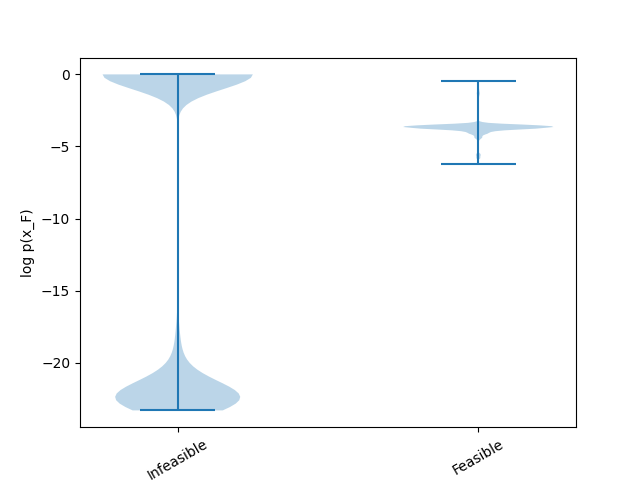
\includegraphics[width=\textwidth]{resources/img/violin_theta_factor/scp_n50_m50_k5.csv.png}
        \caption{$SCP\,(n=50, m=50, k=5)$}
        \label{fig:violin_scp_n50_m50_k5}
    \end{subfigure}
    \hfill
    \begin{subfigure}[b]{0.32\textwidth}
        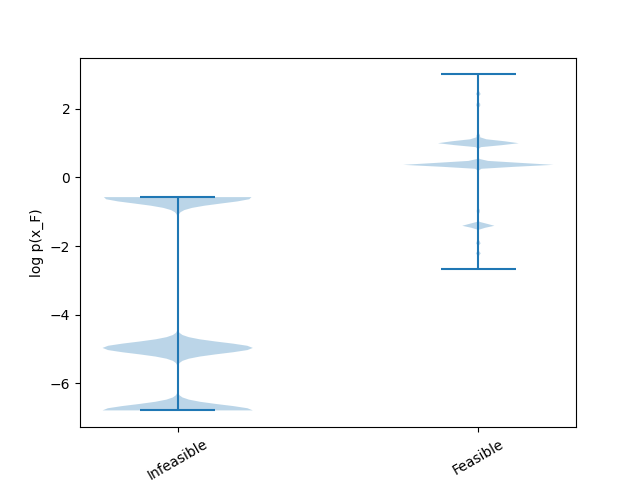
\includegraphics[width=\textwidth]{resources/img/violin_theta_factor/mis_n100_p0.15.csv.png}
        \caption{$MIS\,(n=100, p=0.15)$}
        \label{fig:violin_mis_n100_p0.15}
    \end{subfigure}
    \hfill
    \begin{subfigure}[b]{0.32\textwidth}
        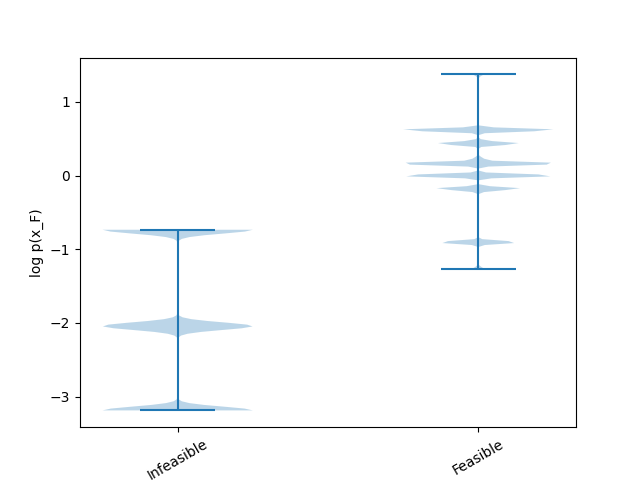
\includegraphics[width=\textwidth]{resources/img/violin_theta_factor/mis_n200:300_p0.15_maxdeg15.csv.png}
        \caption{$MIS\,(n\sim [200,300], p=0.15)$}
        \label{fig:violin_mis_n200:300_p0.15}
    \end{subfigure}
    \caption{Distributions of log-potentials $\EPARAMF(\XFACT)$ predicted by the GNN$+$LBP model and grouped by the feasibility of factor assignments. Overall, feasible assignments receive higher log-probabilities (near $0$) while infeasible ones are mostly suppressed (large negative values). Notably, an island of infeasible assignments attains unexpectedly high scores, overlapping the feasible region—indicating either remaining model misspecification or strong similarity between those infeasible assignments and feasible ones.}
    \label{fig:violin-comparison}
\end{figure}

\todo[inline]{add same violin plots for GNN+NMF models}



\subsection{Discussion}

Across MIS and SCP benchmarks, the main takeaway is clear: replacing factorized logits with an explicitly structured, differentiable MRF and decoding with BP-Guided Decimation (BPGD) systematically improves solution quality over a strong GNN-only baseline, at a modest but controllable runtime cost.

\paragraph{Solution quality.}
On SCP ($n{=}50,m{=}50,k{=}5$), our learned LBP$+$GD reduces the mean optimality gap from $10.92\%$ (GNN) to $1.54\%$ (Table~\ref{tab:lbp_nmf_bpgd_test_gap_results}), confirming that modeling dependencies among sets/items is particularly beneficial for covering constraints. The trend holds on MIS: for $n{=}100$ (ER graphs with $p{=}0.15$), LBP cuts the GNN gap from $14.55\%$ to $8.85\%$, and LBP$+$GD brings it further down to $6.92\%$; for larger MIS graphs ($n{\sim}[200,300]$) the improvement is even more pronounced, dropping from $22.85\%$ (GNN) to $4.71\%$ with LBP$+$GD. These gains are obtained despite fixing the number of BP iterations and using simple four-layer encoders, highlighting that the bulk of the advantage comes from enforcing local consistency through the factor graph.

\paragraph{Runtime–quality trade-off.}
The structured decoders are costlier than a pure greedy pass, but remain inexpensive in absolute terms on the sizes we target. On SCP ($50{\times}50$), moving from GNN ($0.06$s) to LBP$+$GD ($0.404$s) yields an order-of-magnitude reduction in gap for only a few extra tenths of a second (Table~\ref{tab:lbp_nmf_bpgd_test_time_results}). On MIS, LBP$+$GD roughly doubles to triples the runtime compared to GNN (e.g., $0.38$s $\rightarrow$ $0.85$s at $n{=}100$, and $0.98$s $\rightarrow$ $2.08$s at $n{\sim}\mathcal{U}[200,300]$), but delivers large gap reductions. Our frequency-ablation (Fig.~\ref{fig:bp_gap_runtime_split}) shows that running BP every $4$–$8$ decimation steps preserves most of the quality gains while shaving $30\%$–$50\%$ of decoding time, offering a practical knob for deployment under time budgets.

\paragraph{Effect of evidence and guidance.}
BPGD’s advantage over one-shot greedy decoding stems from the ability to clamp partial assignments and re-propagate their impact through constraints. Fig.~\ref{fig:bpgd_delta_marginals} quantifies this: the average change in marginals is small early on (when evidence is weak) and grows later, when conflicts and coverage become decisive. This adaptivity specifically mitigates tie-breaking failures of score-guided greedy methods in mutually exclusive neighborhoods (MIS) and in overlapping, high-coverage sets (SCP).

\paragraph{Comparison to “train-less” canonical MRFs.}
Using hand-crafted canonical parameters (zero for feasible configurations, $-\infty$ for infeasible) with BPGD provides a strong unsupervised baseline (Table~\ref{tab:canonical_mrf_gap_results}). On SCP, our learned LBP$+$GD ($1.54\%$) clearly surpasses canonical LBP$+$GD ($4.03\%$), indicating that parameter learning captures instance-specific structure beyond feasibility. On MIS, the canonical LBP$+$GD is competitive or better at the current capacity/feature budget (e.g., $1.82\%$ vs.\ $6.92\%$ at $n{=}100$, $3.85\%$ vs.\ $4.71\%$ at $n{\sim}\mathcal{U}[200,300]$), suggesting that (i) MIS with pairwise factors already benefits greatly from feasibility propagation, and (ii) our learned parameterization still has headroom—richer embeddings, better calibration of pairwise potentials, or curriculum schedules for BP could close this gap. Importantly, both learned and canonical NMF variants underperform LBP, which aligns with our analysis of mean-field’s inability to reflect degree/overlap effects under homogeneous canonical parameters.

\paragraph{Scalability and limits.}
Even with loopy graphs and fixed iteration budgets, LBP remains stable in practice and scales gracefully in our regime. Absolute solve times stay within seconds on a single GPU and grow smoothly with $n$ (Tables~\ref{tab:lbp_nmf_bpgd_test_time_results},~\ref{tab:canonical_mrf_gap_results}). The main limitations we observe are (i) sensitivity to the number of BP iterations and damping, and (ii) the expressivity/size trade-off of the exponential-family parameterization with over-complete statistics (which grows with factor size). These constraints motivated our focus on MIS and SCP, where factor arity is controlled; generalizing to problems with large or learned higher-order factors will require either structured parameter tying or low-rank/sparse parameterizations.

\section{Conclusion}
It is important to emphasize that the present study was designed primarily to highlight the improvements brought by structured inference (BP) compared to factorized logit predictions. To make this comparison clear and tractable, we deliberately focused on problem families (MIS and SCP) whose natural formulations yield factor graphs with small arity. In this setting, the canonical over-complete parametrization is still feasible to implement, and thus we can study the effect of inference in a controlled environment. Future contributions will move beyond this “idealized” parametrization to problems involving larger factors, where the exponential growth of sufficient statistics makes canonical representations impractical. This shift will require approximate parameterizations, structured factor tying, or low-rank formulations, and will allow us to test the generality of MRF-augmented predictors in more realistic combinatorial optimization tasks.

\paragraph{Take-home messages.}
(i) Structured, differentiable inference (LBP) coupled with BPGD reliably improves over factorized GNN predictors on both packing and covering problems; (ii) the extra cost is small and can be tuned via the BP-frequency knob; (iii) canonical “train-less” MRFs form a strong baseline on MIS, but learning clearly helps on SCP and should help more broadly as parameterizations and features are enriched; and (iv) naïve mean-field is ill-suited here, whereas LBP effectively communicates exclusivity/coverage through the graph. Overall, the results validate MRF-augmented learning as a practical path to higher-quality, feasible solutions in CO, and motivate future work on (a) stronger parameter heads (e.g., degree-aware or message-calibrated potentials), (b) adaptive inference schedules (entropy/variance-triggered updates), and (c) scalable approximations for higher-order factors.





% \chapter{Denoising and MRF inference}\label{chap4:denoising}
% \chaptermark{Denoising and MRF inference}
% \chapter{From Structured Inference to Learned Refinement Dynamics}\label{chapter:4_denoising_and_mrf_inference}
\chaptermark{Learned MRF Refinement}

\section{Introduction}

The previous chapter studied how Markov Random Fields can be used as structured prediction models for binary integer linear programs. Instead of predicting independent variable scores, the models introduced there first predicted or instantiated factor potentials and then used approximate inference to obtain marginals that reflect the dependencies induced by the constraints. These marginals were finally converted into feasible assignments by decoding procedures such as EGG and GD. This showed that graphical-model inference can provide a useful intermediate representation between neural prediction and solution construction.

This chapter moves from structured prediction by inference to structured prediction by iterative refinement. Rather than producing a single set of MRF parameters or variable marginals and decoding them immediately, we train models that define dynamics over candidate solutions. Starting from a noisy, relaxed, or randomly initialized assignment, the model is applied repeatedly so as to transform the current state into a cleaner and more solution-like representation. This viewpoint is motivated by recent denoising, diffusion, and flow-based generative models, but the generated object here is not an image or a continuous signal: it is a candidate solution to a constrained combinatorial optimization problem. As a consequence, the learned trajectory must ultimately be coupled with a decoding step that converts the final state into a feasible binary assignment.

We consider two related families of refinement models. The first family augments the MRF-based architecture of the previous chapter with a flow-based generative objective. Given an initial random assignment and a target solution, we define an interpolation path between the two and train the model either to predict the instantaneous velocity along this path or to predict the clean endpoint directly. In the velocity-prediction setting, the model is trained in a flow-matching fashion: at each time $t$, it receives the current interpolated state and predicts a direction of motion toward the target solution. At test time, generation is performed by initializing from a random Bernoulli distribution and unrolling the learned dynamics for a finite number of steps. In the direct-denoising variant, the model is trained on the same type of intermediate states but predicts the denoised solution itself rather than the velocity.

The second family follows a diffusion-inspired denoising formulation. Clean reference solutions are corrupted according to a forward noising process, and the model is trained to reconstruct the original solution from the corrupted sample, the problem instance, and the noise level. In contrast with the flow-based models, where the interpolation path gives a deterministic relation between the initial and target states, the diffusion-inspired model is trained on independently sampled corruption levels. Thus each minibatch contains reconstruction tasks of different difficulty, ranging from
lightly corrupted solutions to highly noisy samples. This objective encourages the model to learn a denoising rule that is useful across the whole refinement trajectory. 

A central difference between this chapter and the previous one is the role of the test-time budget. In Chapter~\ref{chapter:3_differentiable_mrf_inference_for_bilps}, the main computational trade-off came from the amount and frequency of approximate inference used during Guided Decimation. Here, the learned model itself is iterative: we may decode after a small number of refinement steps, or continue unrolling the dynamics until the terminal time $t=1$. The number of unrolling steps therefore becomes a new control parameter. It affects both runtime and solution quality, and it determines how much of the final solution is produced by the learned refinement dynamics before the feasibility-preserving decoder is applied.

We keep the decoding stage deliberately close to the one used in the previous chapter. After unrolling the flow or denoising model, the final relaxed state is interpreted as a set of variable scores and decoded using the same problem-specific feasibility propagation rules for SC and MIS. This makes the comparison with the previous chapter direct: the main change is not the final decoder, but the way the scores given to the decoder are produced. As before, we evaluate the resulting assignments using relative optimality gap, feasibility, and runtime.

The experiments are conducted on the same two representative problem families: SC and MIS. These problems expose different forms of constraint structure. SC contains covering constraints that allow gradual accumulation of selected sets, while MIS contains exclusion constraints where selecting one vertex immediately rules out its neighbors. This difference turns out to be important. On SC instances, the refinement models provide consistent improvements over the previous prediction methods. On MIS instances, the behavior is more nuanced: some refinement objectives improve the decoded solutions, while others are more sensitive to initialization, unrolling length, and local mistakes in the trajectory.

The main empirical finding of the chapter is that denoising-based refinement is a strong mechanism for solution prediction. The MRF-augmented flow models show
that learned continuous-time dynamics can be used to produce useful decoding signals from random Bernoulli initializations. However, the diffusion-inspired
denoising model is the most robust of the refinement approaches studied here and outperforms most of the models introduced so far. This suggests that training on a range of independently sampled corruption levels provides a more stable learning signal than relying only on a single interpolation-based velocity target.

The contributions of this chapter are as follows:
\begin{enumerate}
    \item We introduce MRF-augmented flow models for binary combinatorial optimization, trained either by velocity prediction or by direct denoising of intermediate states.

    \item We adapt diffusion-inspired denoising to the same BILP solution-prediction setting, using independently sampled timesteps and a reconstruction objective over corrupted reference solutions.

    \item We define a decoding protocol in which samples are initialized from a random Bernoulli distribution, refined by unrolling the learned dynamics, and then converted into feasible assignments using the decoding procedures introduced in Chapter~\ref{chapter:3_differentiable_mrf_inference_for_bilps}.

    \item We study the effect of the unrolling budget on solution quality and runtime, highlighting the difference between partial refinement and full unrolling to $t=1$.

    \item We evaluate the proposed models on SC and MIS instances, showing consistent gains on SC, more complex behavior on MIS, and strong overall performance for the diffusion-inspired denoising architecture.
\end{enumerate}

\paragraph{Positioning with respect to Chapter~3}
Chapter~\ref{chapter:3_differentiable_mrf_inference_for_bilps} used MRF inference as a structured prediction layer: a neural model predicted factor potentials, approximate inference transformed these potentials into marginals, and a decoder converted the resulting scores into a feasible assignment. The present chapter keeps the same general goal of producing constraint-aware decoding signals, but changes the role of the model. Instead of using inference to produce a single set of marginals before or during decoding, we train models that define an iterative refinement process over candidate solutions. The MRF-augmented flow and denoising models therefore shift the emphasis from \emph{structured marginal prediction} to \emph{structured trajectory learning}. This also changes the test-time trade-off: in Chapter~3 the main budget was the number and frequency of inference calls, whereas here the main budget is the number of refinement steps before decoding. The chapter can thus be read as a continuation of the previous one: it asks whether the structured information provided by MRF-based representations can be combined with denoising and flow-style dynamics to obtain better solution predictions than a single inference-and-decode pass.

\section{MRF-Augmented Flow Models}

The previous chapter used MRF inference as a structured prediction layer: a neural network predicted factor parameters, approximate inference transformed these
parameters into marginal beliefs, and a decoder converted the resulting scores into a feasible assignment. In this section we introduce a refinement-based variant of the same idea. Instead of applying the model once to an instance, we condition the model on a current candidate solution state and use it to define an iterative transformation from a simple source distribution toward a solution-like endpoint.

The construction is inspired by flow matching and rectified-flow models, which learn time-dependent vector fields transporting samples from a source distribution to a data distribution \citep{lipman_flow_2022,liu_flow_2022,tong_improving_2023}. In our setting, however, the transported object is not a continuous data point such as an image. It is a relaxed representation of a binary solution to a BILP. The learned trajectory therefore lives in $[0,1]^n$, and the endpoint must still be decoded into a binary feasible assignment.

We consider a supervised setting in which each training instance $\PROB$ is associated with a reference solution $y\in\{0,1\}^n$. A source state $z$ is sampled from a simple distribution over relaxed or binary assignments, and a time $t\in[0,1]$ is sampled independently of the instance data. The model receives the original instance together with an interpolated state $p_t$ and predicts either a denoised endpoint or a velocity derived from this endpoint. When the model is MRF-augmented, the prediction is not only a vector of independent variable scores: the graph encoder predicts factor parameters, LBP or NMF is run on the resulting factor graph, and the unary marginals are used as the denoised variable probabilities.

\subsection{Refinement states and initialization}

Let $\PROB$ be a BILP instance with $n$ binary decision variables and let $y\in\{0,1\}^n$ denote a reference solution. We define a continuous relaxation of the
solution space by representing an assignment through a vector
\begin{equation*}
    p \in [0,1]^n,
\end{equation*}
where $p_i$ is interpreted as the current probability or relaxed value assigned to $x_i=1$.

The source state $z$ is sampled componentwise from a simple distribution. In the implementation, two source distributions are supported:
\begin{equation}
    z_i \sim \mathcal{U}(0,1) \qquad\text{or}\qquad z_i \sim \mathrm{Bernoulli}(\rho),
\end{equation}
where $\rho$ is a configurable source probability, typically $\rho=1/2$. The uniform source is the default in our implementation, while the Bernoulli source corresponds to the purely binary random initialization used in some evaluations. Both choices play the same conceptual role: they provide an unstructured initial state from which the model must recover a solution-like representation.

Given $z$, $y$, and a time $t\in[0,1]$, we use the linear probability path
\begin{equation}
    p_t = (1-t)z + t y .
    \label{eq:flow_probability_path}
\end{equation}
Thus $p_0=z$ and $p_1=y$. Intermediate values $p_t$ are relaxed assignments in $[0,1]^n$. This path is the analogue, in the relaxed binary solution space, of the straight interpolation paths used in rectified flow and conditional flow matching.

During training, times are sampled either per problem or per variable. In the per-problem setting, a single time $t$ is sampled for each BILP instance in the minibatch and shared by all its variables. In the per-variable setting, each variable receives its own independently sampled time. Unless otherwise stated, we use the per-problem variant, since it gives each instance a coherent global noise or refinement level.

To condition the neural model on the current refinement state, we augment the variable--constraint graph representation of $P$. For every variable node $i$, we append the current value $p_{t,i}$ to its feature vector. When enabled, we also append the time value $t_i$. Constraint nodes receive zeros in these appended feature dimensions. The resulting graph is denoted
\begin{equation}
    \VCG_t = \mathrm{Augment}(\VCG, p_t, t),
\end{equation}
where $\VCG$ is the original variable--constraint graph. The implementation also stores $p_t$, $t$, and the source state $z$ with the augmented batch, because these quantities are needed to form the supervised flow targets. This matches the implementation, where flow features are appended only to variable nodes and where the batch stores $p_t$, $t$, and $z$ for the loss and rollout computations.

At test time, the same representation is used iteratively. We sample an initial state $p^{(0)}=z$, build the augmented graph $\VCG_{t_0}$, evaluate the model, update the state, and repeat this procedure for a fixed number of unrolling steps. The number of steps is therefore a test-time refinement budget. Larger budgets allow the model to move farther along the learned trajectory, but also increase the cost of producing the scores used by the final decoder.

\subsection{Velocity Prediction by Flow Matching}

The first training objective follows the flow-matching viewpoint. Along the linear path in Equation~\eqref{eq:flow_probability_path}, the ideal velocity is
\begin{equation}
    u_t = \frac{d p_t}{dt} = y - z .
    \label{eq:flow_target_velocity}
\end{equation}
This target does not depend on $t$ for the linear path, but the model must infer it from the current state $p_t$, the time $t$, and the problem instance $\PROB$.

Let $F_\omega$ denote the MRF-augmented flow model. Given the augmented graph $\VCG_t$, the model produces an estimate of the clean endpoint,
\begin{equation}
    \widehat q_1 = F_\omega(\VCG_t) \in [0,1]^n .
\end{equation}
When the model is an MRF model, this vector is obtained from the inferred unary marginals:
\begin{equation}
    \widehat q_{1,i} = \widehat\MARGINAL_i(x_i=1).
\end{equation}
The endpoint estimate can be converted into an instantaneous velocity at time $t$ by asking which velocity would move the current point $p_t$ to the predicted endpoint at time $1$:
\begin{equation}
    \widehat v_t = \frac{\widehat q_1 - p_t}{1-t}.
    \label{eq:endpoint_to_velocity}
\end{equation}
For numerical stability, the denominator is clipped below by a small constant $\varepsilon>0$ in the implementation.

The instantaneous-velocity objective is therefore
\begin{equation}
    \mathcal{L}_{\mathrm{FM}}(\omega) = \mathbb{E}_{(P,y),\,z,\,t}
    \left[
        \ell\!\left(
            \frac{F_\omega(H_t)-p_t}{\max(1-t,\varepsilon)},
            y-z
        \right)
    \right],
    \label{eq:instant_velocity_loss}
\end{equation}
where $\ell$ is a regression loss, such as mean-squared error or $\ell_1$ loss. 

At inference time, we integrate the learned dynamics by an explicit Euler scheme. Starting from $p^{(0)}=z$, choose a grid
\begin{equation}
    0=t_0<t_1<\cdots<t_K=t_{\mathrm{end}}\leq 1,
\end{equation}
and let $\Delta t_k=t_{k+1}-t_k$. At step $k$, the model predicts an endpoint estimate $\widehat q_1^{(k)}=F_\omega(H_{t_k})$, which is converted into a velocity
\begin{equation}
    \widehat v_{t_k} = \frac{\widehat q_1^{(k)}-p^{(k)}}{\max(1-t_k,\varepsilon)}.
\end{equation}
The relaxed assignment is then updated as
\begin{equation}
    p^{(k+1)} = \Pi_{[0,1]^n}
    \left(
        p^{(k)} + \Delta t_k \widehat v_{t_k}
    \right),
    \label{eq:flow_euler_update}
\end{equation}
where $\Pi_{[0,1]^n}$ denotes coordinatewise clipping to the interval $[0,1]$.

\subsection{Direct Denoising Along the Flow Path}

The second objective uses the same interpolation path but changes the supervision target. Instead of training the model to match the velocity, we train it to predict the clean endpoint directly. The model receives the same input $\VCG_t$, containing the problem instance, the current relaxed state $p_t$, and the time $t$, but the target is now the reference solution $y$:
\begin{equation}
    F_\omega(H_t) \approx y .
\end{equation}
The corresponding denoising loss is
\begin{equation}
    \mathcal{L}_{\mathrm{denoise}}(\omega)
    =
    \mathbb{E}_{(P,y),\,z,\,t}
    \left[
        \ell\!\left(F_\omega(H_t), y\right)
    \right].
    \label{eq:flow_denoising_loss}
\end{equation}
When the model outputs logits, $\ell$ is a binary cross-entropy loss. When the model outputs probabilities or MRF marginals, $\ell$ can be a mean-squared error, an $\ell_1$ loss, or the variational cross-entropy loss used for marginal-based models.

Although the training target is different, the test-time rollout can still use the same endpoint-velocity update as in Equation~\eqref{eq:flow_euler_update}. The reason is that an endpoint predictor implicitly defines a velocity field: if the model believes that the terminal state should be $\widehat q_1$, then the straight-line velocity from the current state $p_t$ to that endpoint is $(\widehat q_1-p_t)/(1-t)$. Thus the direct denoising model is trained as an endpoint predictor but can be unrolled as a flow model.

\subsection{Architecture and MRF-Augmented State Representation}

The MRF-augmented flow architecture reuses the structured prediction pipeline from Chapter~\ref{chapter:3_differentiable_mrf_inference_for_bilps}, with one additional input: the current refinement state. The original BILP instance is represented by its variable--constraint graph $\VCGFULL$ where variable nodes correspond to decision variables and constraint nodes correspond to linear constraints. At time $t$, the graph is augmented into $\VCG_t$ by appending the
current state $p_t$ and the time $t$ to the variable-node features.

The graph encoder processes $\VCG_t$ and produces node embeddings. These embeddings are then mapped to MRF factor parameters. As in Chapter~3, unary factors are associated with variable nodes and non-unary factors with constraint nodes. The model therefore defines a time-dependent MRF
\begin{equation}
    p_{\theta_\omega(t,p_t,\PROB)}(x\mid \PROB,p_t,t)
    \propto
    \exp\left(
        \sum_{\alpha\in F}
        \left\langle
            \theta_{\omega,\alpha}(\PROB,p_t,t),
            \phi_\alpha(x_\alpha)
        \right\rangle
    \right),
    \label{eq:flow_time_dependent_mrf}
\end{equation}
where the factor parameters now depend not only on the instance $\PROB$, but also on the current refinement state $p_t$ and the time $t$.

Approximate inference is then applied to this time-dependent MRF. With LBP, the model returns approximate unary beliefs $\widehat\MARGINAL_i(x_i)$ after a fixed number of message-passing iterations. With NMF, it returns the corresponding factorized marginals. In both cases, the flow score used by the rollout is
\begin{equation}
    \widehat q_{1,i}
    =
    \widehat\MARGINAL_i(x_i=1).
    \label{eq:flow_score_from_marginal}
\end{equation}
Thus, the endpoint estimate is not produced independently for each variable: it is the result of running approximate inference in a factor graph whose potentials are conditioned on the current state of the refinement trajectory.

This architecture leads to two related evaluation modes. In the first mode, we run a flow rollout once, obtain a final relaxed state $p^{(K)}$, make one final model call at the projection time, and then decode the resulting scores using EGG or GD. In the second mode, used by the flow-conditioned GD backend, the decoder itself calls a flow-conditioned inference backend. Each time GD requests new beliefs, the backend constructs a source state consistent with the current decimation evidence, runs a full flow rollout, extracts the final MRF parameters, applies the evidence mask, and then runs LBP or NMF. This makes the flow model conditional not only on the original instance, but also on the partial assignment accumulated by the decoder.

More explicitly, suppose that GD has already fixed a partial assignment $S\subseteq V\times\{0,1\}$. The evidence-aware source distribution enforces
\begin{equation}
    z_i =
    \begin{cases}
        0, & (i,0)\in S,\\
        1, & (i,1)\in S,\\
        \text{random}, & i \text{ unfixed}.
    \end{cases}
\end{equation}
The flow rollout is then initialized from this evidence-aware source. After the rollout, the predicted factor parameters are masked so that assignments inconsistent with the current evidence receive negligible probability, and LBP or NMF is run on the conditioned MRF. The resulting beliefs are returned to the same decimation rule used in Chapter~3.

This gives the model two mechanisms for incorporating structure. First, the neural network observes the current relaxed assignment through the appended flow features. Second, the MRF layer propagates the resulting local factor information through LBP or NMF before the decoder chooses the next variables to fix. The flow model therefore acts as a learned refinement map over solution states, while the MRF layer preserves the constraint-aware inference mechanism introduced in the previous chapter.

\section{Diffusion-Inspired Denoising Model}

The flow models introduced in the previous section define a deterministic refinement path between a simple source state and a reference solution. We now consider a second refinement strategy, inspired by denoising diffusion models. The central idea is to train a model to recover a clean solution from a corrupted one. Instead of learning a velocity field along an interpolation path, the model is exposed to noisy versions of reference solutions and is trained to predict the original assignment.

This approach is particularly natural for binary combinatorial optimization. A solution can be represented as a binary vector $y\in\{0,1\}^n$, and corruption can be interpreted as randomly destroying part of the information contained in this vector. The denoising model must then infer which variables should be selected by using both the corrupted assignment and the structure of the optimization instance. In this sense, denoising is not merely a variable-wise reconstruction task: the model must learn how feasibility constraints and objective information restrict the set of plausible clean solutions.

Diffusion-based approaches have recently been adapted to combinatorial optimization by treating candidate solutions as discrete or relaxed objects that can be
gradually corrupted and reconstructed \citep{sun_difusco_2023}. The model studied here follows this general perspective, but we use it primarily as a learned denoising mechanism for producing solution scores. The final output is still decoded using the same feasibility-preserving procedures as in the previous models. Thus, as with the flow-based approach, the denoising model produces a structured prediction signal, while the decoder is responsible for converting this signal into a feasible binary assignment.

\subsection{Forward Corruption Process}

Let $P$ be a BILP instance and let $y\in\{0,1\}^n$ be a reference solution. The forward corruption process defines a family of noisy assignments
\begin{equation}
    y_t \sim q(\cdot \mid y,t),
\end{equation}
indexed by a discrete timestep $t\in\{0,\ldots,T-1\}$. Small timesteps correspond to lightly corrupted solutions, while large timesteps correspond to states in which much of the information about the original solution has been removed.

We consider a corruption process acting independently on the components of the solution vector. For each variable $i$, the clean value $y_i$ is either kept or corrupted according to a timestep-dependent noise level. A convenient form is a replacement corruption:
\begin{equation}
    y_{t,i}
    =
    \begin{cases}
        y_i, & \text{with probability } \bar{\alpha}_t,\\
        \xi_i, & \text{with probability } 1-\bar{\alpha}_t,
    \end{cases}
    \qquad
    \xi_i \sim \mathrm{Bernoulli}(1/2),
    \label{eq:diffusion_replace_corruption}
\end{equation}
where $\bar{\alpha}_t$ is a decreasing signal-preservation coefficient. At early timesteps, $\bar{\alpha}_t$ is close to one, so the corrupted sample remains close to the reference solution. At late timesteps, $\bar{\alpha}_t$ is smaller, and many variables are replaced by random binary values.

An alternative corruption mechanism is bit-flipping:
\begin{equation}
    y_{t,i}
    =
    \begin{cases}
        1-y_i, & \text{with probability } \beta_t,\\
        y_i, & \text{with probability } 1-\beta_t,
    \end{cases}
    \label{eq:diffusion_flip_corruption}
\end{equation}
where $\beta_t$ increases with $t$. Both views define a sequence of reconstruction tasks of increasing difficulty. The replacement corruption is closer to a masking or information-destruction process, while the flipping corruption creates adversarially wrong binary values. In both cases, the model observes a corrupted solution and must infer a plausible clean assignment from the instance structure.

The noise schedule controls how quickly information is destroyed as $t$ increases. For example, one may use a linear schedule, where the corruption level increases at a constant rate, or a smoother nonlinear schedule that corrupts the solution more slowly at the beginning and more strongly near the end. The precise schedule is a hyperparameter of the method. Its role is to distribute training examples across different noise levels, so that the denoiser learns both local repair of nearly correct solutions and global reconstruction from highly noisy inputs.

The corrupted vector $y_t$ is then provided to the model as an additional variable-level signal. Conceptually, the input at timestep $t$ is the pair
\begin{equation*}
    (\PROB,y_t,t),
\end{equation*}
where $\PROB$ gives the optimization instance, $y_t$ gives the current noisy assignment, and $t$ indicates the corruption level. The model must combine these three sources of information: the graph structure and coefficients of the instance, the current state of the candidate solution, and the amount of noise that has been applied.

\subsection{Denoising Objective}

The denoising model is trained to reconstruct the clean solution from its corrupted version. Let
\begin{equation*}
    D_\omega(\PROB,y_t,t)
\end{equation*}
denote the model prediction at timestep $t$. Depending on the architecture, this prediction may be a vector of variable logits, variable probabilities, or MRF-derived marginals. In all cases, the output is interpreted as a score indicating whether each variable should be set to one in the clean solution.

The basic denoising objective is
\begin{equation}
    \mathcal{L}_{\mathrm{diff}}(\omega)
    =
    \mathbb{E}_{(P,y),\,t,\,y_t\sim q(\cdot\mid y,t)}
    \left[
        \ell\bigl(D_\omega(P,y_t,t),y\bigr)
    \right],
    \label{eq:diffusion_denoising_loss}
\end{equation}
where $\ell$ is a reconstruction loss. For binary outputs, a natural choice is the componentwise binary cross-entropy:
\begin{equation}
    \ell(\hat{p},y)
    =
    -
    \sum_{i=1}^n
    \left[
        y_i\log \hat{p}_i
        +
        (1-y_i)\log(1-\hat{p}_i)
    \right],
    \label{eq:diffusion_bce}
\end{equation}
where $\hat{p}_i$ is the predicted probability that $x_i=1$. When the model produces MRF marginals, $\hat{p}_i$ corresponds to the inferred unary belief $\hat{\mu}_i(x_i=1)$. Other reconstruction losses can also be used when the output is treated as a relaxed probability vector.

This objective differs from the velocity-prediction objective of the flow model. In flow matching, the target is a direction of motion along a path from noise to data. In the diffusion-inspired denoising model, the target is always the clean solution itself. The timestep changes the difficulty of the reconstruction problem, but not the object being predicted. The model is therefore trained to answer the question: given this instance and this corrupted assignment, what clean solution is most plausible?

At test time, the denoising model can be used in several ways. The simplest use is one-shot denoising: a noisy assignment is provided at a chosen timestep, the model predicts clean variable scores, and these scores are decoded into a feasible solution. A more generative use applies the denoiser iteratively. Starting from a highly corrupted or random assignment, the model is evaluated at decreasing timesteps, producing a sequence
\begin{equation}
    y_T \rightarrow y_{T-1} \rightarrow \cdots \rightarrow y_0 .
\end{equation}
At each step, the model prediction defines a new candidate assignment, either by thresholding the predicted probabilities or by sampling from them. The final state is then passed to the same feasibility-preserving decoder used for the other models.

This iterative procedure should be understood as a learned refinement heuristic rather than an exact reverse diffusion sampler. The model is trained to reconstruct clean solutions from noisy inputs, and repeated application of this denoising rule provides a way to progressively transform an unstructured binary state into a more solution-like one. The final feasibility and objective quality are then determined by the interaction between the denoising trajectory and the downstream decoder.

\subsection{Independent Timestep Sampling}

A key design choice is how timesteps are sampled during training. Rather than training on a fixed corruption level, we sample timesteps independently for the training examples. This means that each minibatch contains a mixture of reconstruction tasks: some samples are only slightly corrupted, while others are heavily corrupted. The training objective can therefore be written as
\begin{equation}
    \mathcal{L}_{\mathrm{diff}}(\omega)
    =
    \mathbb{E}_{(P,y)}
    \mathbb{E}_{t\sim \mathcal{U}\{0,\ldots,T-1\}}
    \mathbb{E}_{y_t\sim q(\cdot\mid y,t)}
    \left[
        \ell\bigl(D_\omega(P,y_t,t),y\bigr)
    \right].
    \label{eq:diffusion_independent_t_loss}
\end{equation}

This sampling strategy has two advantages. First, it prevents the model from specializing to a single noise level. The denoiser must learn both small corrective
moves near the data distribution and larger reconstruction moves from strongly corrupted assignments. Second, it makes the training signal more diverse: variables and instances are observed under many different corruption patterns, forcing the model to rely on the optimization structure rather than memorizing a fixed perturbation pattern.

In the context of combinatorial optimization, this is especially useful because different noise levels correspond to different algorithmic regimes. At low noise, the task resembles local repair: most variables are already correct, and the model must identify the few components that are inconsistent with the learned solution structure. At high noise, the task resembles solution construction: the corrupted assignment may contain little reliable information, and the model must infer a high-quality assignment mostly from the instance itself. Training across the full range of timesteps therefore encourages a single model to act both as a repair heuristic and as a global predictor.

The timestep is also provided to the model as part of the input. This allows the same network to adapt its behavior to the corruption level. For small $t$, the denoiser can trust the input assignment more strongly and focus on correcting local errors. For large $t$, it should rely more heavily on the graph representation, objective coefficients, and constraint structure of the instance. The timestep-conditioned model therefore learns a family of denoising maps indexed by the corruption level:
\begin{equation}
    D_\omega(\cdot,\cdot,0),
    D_\omega(\cdot,\cdot,1),
    \ldots,
    D_\omega(\cdot,\cdot,T-1).
\end{equation}

This independent timestep sampling distinguishes the diffusion-inspired model from the flow models of the previous section. The flow models are trained along an
interpolation path between a sampled source state and a reference solution. The diffusion-inspired model is trained on corrupted versions of the reference solution itself, with the corruption level sampled independently for each training example. Empirically, this produces a robust denoising signal and gives the model a broad range of refinement behaviors, from local correction to near-complete reconstruction.

\section{Decoding by Unrolling and Feasibility-Preserving Rounding}

The flow and denoising models described above produce relaxed solution states or variable scores. These outputs are not, by themselves, guaranteed to be feasible binary solutions of the original BILP. As in the previous chapter, we therefore separate \emph{prediction} from \emph{decoding}. The learned refinement model produces a score vector, while a feasibility-preserving decoder converts this vector into a valid assignment.

This separation is important for two reasons. First, the intermediate states of the flow and denoising processes lie in a relaxed or noisy space: they may contain fractional values, stochastic samples, or assignments that violate constraints. Second, the decoding procedure allows us to compare the refinement models fairly with the models introduced in Chapter~3. We keep the final decoding mechanisms fixed and study how the quality of the scores changes when they are produced by iterative refinement rather than by a single prediction or inference pass.

The decoding pipeline used in this chapter has three stages. We first initialize a candidate state from a simple random distribution. We then unroll the learned flow or denoising dynamics for a prescribed number of steps. Finally, we interpret the resulting state as variable scores and apply the same feasibility-preserving decoders as before.

\subsection{Random Bernoulli Initialization}

At test time, the refinement process starts from an unstructured relaxed assignment.
Unless otherwise stated, we sample
\begin{equation}
    p^{(0)}_i \sim \mathcal{U}(0,1),
    \qquad i=1,\ldots,n.
    \label{eq:uniform_initialization}
\end{equation}
The initial vector therefore lies in $[0,1]^n$ and can be interpreted as a random probability vector over the binary variables. This initialization contains no information about the instance beyond the number of variables. It tests whether the learned dynamics can transform a random relaxed state into a useful prediction signal for the decoder.

For the flow models, the random vector is interpreted as the initial point of the trajectory:
\begin{equation}
    p^{(0)} = x^{(0)}.
\end{equation}
The model is then unrolled forward in time, producing a sequence of relaxed probability vectors
\begin{equation}
    p^{(0)}, p^{(1)}, \ldots, p^{(K)} \in [0,1]^n.
\end{equation}
For the diffusion-inspired denoising model, the same random initialization can be viewed as a highly corrupted assignment. The denoising model is then applied iteratively at decreasing timesteps, producing a sequence of increasingly refined candidate states.

This random initialization makes the evaluation genuinely generative: the model is not simply repairing a perturbed version of the reference solution. It must produce useful scores from a state that is initially unrelated to the target assignment. In some diagnostic evaluations, we also initialize from corrupted reference solutions in order to measure denoising ability under controlled noise levels. However, the main solution-generation setting starts from random Bernoulli samples.

\subsection{Full and Partial Unrolling}

A distinctive feature of the models in this chapter is that prediction quality depends on the number of refinement steps. Let $K$ denote the number of unrolling steps. For the flow models, we choose a time grid
\begin{equation}
    0=t_0<t_1<\cdots<t_K=t_{\mathrm{end}},
\end{equation}
and apply the learned update rule along this grid. For the diffusion-inspired model, we apply the denoiser over a sequence of timesteps, typically from a high-noise state toward a low-noise state.

When $t_{\mathrm{end}}=1$, the flow model is fully unrolled to the terminal time. We refer to this setting as \emph{full unrolling}. The resulting vector is intended to approximate the endpoint of the learned transport process. In contrast, \emph{partial unrolling} stops the dynamics earlier, with $t_{\mathrm{end}}<1$ or with fewer refinement steps. The decoder is then applied to an intermediate state.

Partial unrolling is useful for two reasons. First, it defines a runtime--quality trade-off. Fewer refinement steps reduce inference time, but may provide weaker scores. Second, the best decoded solution need not always be obtained after the longest possible rollout. In discrete optimization, a relaxed trajectory can drift toward high-confidence but structurally poor assignments, especially when the model is iterated beyond the regime in which it was most accurate. Evaluating several unrolling budgets therefore allows us to study whether refinement improves monotonically or whether early decoding can sometimes be preferable.

The generic unrolling-and-decoding procedure is summarized in Algorithm~\ref{alg:unroll_decode}.

\begin{algorithm}[t]
\caption{Unrolling and feasibility-preserving decoding}
\label{alg:unroll_decode}
\DontPrintSemicolon

\KwIn{Problem instance $P$, learned refinement model $R_\omega$, number of unrolling steps $K$, decoder $\mathrm{Dec}$}
\KwOut{Feasible assignment $\hat{x}$}

Sample an initial relaxed state $p^{(0)} \sim \mathcal{U}(0,1)^n$\;
$s^{(0)} \leftarrow p^{(0)}$\;

\For{$k \leftarrow 0$ \KwTo $K-1$}{
    Compute the current timestep $t_k$\;
    Predict a refined state or update using $R_\omega(P,s^{(k)},t_k)$\;
    Update the current state to obtain $s^{(k+1)}$\;
}

Interpret $s^{(K)}$ as variable scores\;
$\hat{x} \leftarrow \mathrm{Dec}(P,s^{(K)})$\;

\Return{$\hat{x}$}\;

\end{algorithm}

\section{Main Results}

We now report the main experimental results for the flow-based refinement models. The results are summarized in Table~\ref{tab:flow_inference_results}. We compare direct variable-score flow models, denoted DGN, with MRF-augmented flow models using either LBP or NMF inference. The suffix ``-v'' denotes models trained with the velocity-prediction objective, while the suffix ``-q'' denotes models trained to predict the denoised endpoint directly.

For each model, we report three decoding variants. First, the raw rollout sample is evaluated for feasibility before any feasibility-preserving projection is applied. This measures whether the learned refinement dynamics themselves tend to produce valid assignments. Second, the final rollout state is decoded with EGG, which uses the scores produced after the rollout but does not update them during the construction process. Third, the final rollout state is decoded with GD, which uses the same feasibility-preserving decimation procedure with score updates. For MRF-augmented models, we additionally report a backend GD variant, in which the flow-conditioned MRF signal is recomputed during decimation.

Across the experiments, the most consistent pattern is that MRF-augmented flow models produce substantially better decoding signals than direct variable-score flow models. This is especially clear on Set Cover, where the FMRF-LBP variants achieve low relative gaps and high raw-sample feasibility. The difference between velocity prediction and direct endpoint denoising is generally smaller than the difference between factorized prediction and MRF-augmented prediction, suggesting that the structured inference layer is the main source of improvement in these experiments.

\begin{table}[htbp]
\centering
\resizebox{\textwidth}{!}{
\begin{tabular}{l
                    l
                    S[table-format=2.3]
                    S[table-format=2.3(2.3)]
                    S[table-format=2.3(2.3)]
                    S[table-format=2.3(2.3)]
                    S[table-format=2.3(2.3)]
                    S[table-format=2.3(2.3)]
                    S[table-format=2.3(2.3)]}
        \toprule
        \multirow{2}{*}{\textbf{Dataset}} & \multirow{2}{*}{\textbf{Model}} & \multicolumn{1}{c}{\multirow{2}{*}{\textbf{Feas.} (\%) $\uparrow$}} & \multicolumn{2}{c}{\textbf{EGG}} & \multicolumn{2}{c}{\textbf{GD}} &  \multicolumn{2}{c}{\textbf{FGD}} \\
        \cmidrule(lr){4-5} \cmidrule(lr){6-7} \cmidrule(lr){8-9}
        & & & \multicolumn{1}{c}{Rel. gap (\%) $\downarrow$} & \multicolumn{1}{c}{$t$ (s) $\downarrow$} & \multicolumn{1}{c}{Rel. gap (\%) $\downarrow$} & \multicolumn{1}{c}{$t$ (s) $\downarrow$} & \multicolumn{1}{c}{Rel. gap (\%) $\downarrow$} & \multicolumn{1}{c}{$t$ (s) $\downarrow$} \\
        \midrule
        \multirow{6}{*}{SC-S} & DGN-v & 12.600 & 13.856 (9.525) & \B 0.175 (0.400) & \multicolumn{1}{c}{--} & \multicolumn{1}{c}{--} & 25.978 (11.688) & \B 1.376 (0.393) \\
         & DGN-q & 7.067 & 12.200 (8.531) & 0.193 (0.396) & \multicolumn{1}{c}{--} & \multicolumn{1}{c}{--} & 11.818 (8.469) & 1.743 (0.398) \\
         & FMRF-LBP-v & 64.635 & 2.428 (4.749) & 0.652 (0.383) & 2.353 (4.704) & 1.004 (0.443) & 1.384 (4.165) & 4.848 (1.440) \\
         & FMRF-LBP-q & \B 67.000 & \B 2.337 (4.625) & 0.634 (0.381) & \B 2.312 (4.622) & 0.951 (0.426) & \B 1.308 (3.876) & 4.711 (1.238) \\
         & FMRF-NMF-v & 29.667 & 3.921 (5.526) & 0.425 (0.369) & 2.953 (5.182) & \B 0.567 (0.373) & 2.400 (4.644) & 3.426 (0.496) \\
         & FMRF-NMF-q & 18.800 & 3.853 (5.356) & 0.403 (0.371) & 3.116 (5.005) & 0.590 (0.375) & 2.873 (5.001) & 4.560 (0.390) \\
        \midrule
        \multirow{6}{*}{SC-M} & DGN-v & 0.000 & 14.411 (4.811) & 0.653 (0.353) & \multicolumn{1}{c}{--} & \multicolumn{1}{c}{--} & 13.670 (5.064) & 4.974 (0.777) \\
         & DGN-q & 0.000 & 15.838 (5.237) & \B 0.635 (0.364) & \multicolumn{1}{c}{--} & \multicolumn{1}{c}{--} & 16.097 (5.554) & \B 4.566 (0.699) \\
         & FMRF-LBP-v & \B 80.690 & 2.938 (2.843) & 1.699 (0.710) & 2.938 (2.839) & 1.916 (0.726) & 4.426 (3.518) & 10.440 (1.763) \\
         & FMRF-LBP-q & 68.735 & \B 2.893 (2.928) & 1.663 (0.694) & 2.893 (2.928) & 1.876 (0.703) & \B 4.406 (3.489) & 10.356 (1.563) \\
         & FMRF-NMF-v & 61.867 & 6.642 (3.517) & 1.314 (0.513) & \B 6.647 (3.504) & \B 1.507 (0.522) & 6.206 (3.629) & 5.978 (0.964) \\
         & FMRF-NMF-q & 28.287 & 6.734 (3.514) & 1.303 (0.581) & 6.739 (3.522) & 1.668 (0.587) & 12.421 (4.883) & 9.734 (1.372) \\
        \midrule
        \multirow{6}{*}{MIS-S} & DGN-v & 0.000 & 23.256 (6.135) & \B 0.566 (0.503) & \multicolumn{1}{c}{--} & \multicolumn{1}{c}{--} & 23.065 (6.172) & \B 1.307 (0.496) \\
         & DGN-q & 21.000 & 22.354 (6.226) & 0.576 (0.495) & \multicolumn{1}{c}{--} & \multicolumn{1}{c}{--} & 21.371 (6.085) & 1.355 (0.499) \\
         & FMRF-LBP-v & \B 62.933 & 18.376 (6.522) & 1.192 (0.494) & 19.778 (6.755) & 1.370 (0.496) & \B 20.360 (5.456) & 4.913 (0.512) \\
         & FMRF-LBP-q & 55.067 & \B 14.311 (5.604) & 1.194 (0.496) & \B 18.188 (7.377) & 1.328 (0.496) & 21.148 (5.678) & 4.765 (0.506) \\
         & FMRF-NMF-v & 5.000 & 24.736 (6.216) & 0.780 (0.569) & 39.960 (5.015) & \B 0.829 (0.566) & 41.945 (4.476) & 1.996 (0.566) \\
         & FMRF-NMF-q & 4.067 & 24.398 (6.222) & 0.779 (0.572) & 38.514 (5.231) & 0.831 (0.571) & 40.471 (4.675) & 2.026 (0.566) \\
        % \midrule
        % \multirow{6}{*}{MIS-M} & DGN-v &  &  &  &  &  &  &  \\
        %  & DGN-q &  &  &  &  &  &  &  \\
        %  & FMRF-LBP-v &  &  &  &  &  &  &  \\
        %  & FMRF-LBP-q &  &  &  &  &  &  &  \\
        %  & FMRF-NMF-v &  &  &  &  &  &  &  \\
        %  & FMRF-NMF-q &  &  &  &  &  &  &  \\
        \bottomrule
    \end{tabular}}

\caption{Flow inference performance across datasets and models. ``Feas.'' denotes the proportion of samples obtained after unrolling the flow that satisfy the problem feasibility constraints. For each decoding method---EGG, GD, and FGD---the table reports the average relative optimality gap and runtime, with values in parentheses indicating the corresponding standard deviations.}
\label{tab:flow_inference_results}
\end{table}


\subsection{Set Cover Results}

The Set Cover results show a clear advantage for the MRF-augmented flow models. On SC-S, the direct DGN flow baselines obtain EGG and GD gaps above $12\%$, whereas the FMRF-LBP variants reduce the gap to approximately $2.3$--$2.4\%$ with EGG and GD. The FMRF-NMF variants also improve over DGN, although their gaps remain higher than those of FMRF-LBP. This indicates that the learned flow trajectory benefits from structured inference, and that LBP provides a stronger decoding signal than the fully factorized NMF approximation in this setting.

The raw feasibility rate also increases sharply when using MRF-augmented models. For SC-S, the DGN variants produce feasible rollout samples in only a small fraction of cases, while FMRF-LBP produces feasible samples in more than half of the test instances. This is an important observation: although feasibility is ultimately enforced by the decoder, the learned MRF-augmented dynamics already move the relaxed state toward assignments that are much more compatible with the constraints.

The same trend appears on SC-M. The DGN baselines have gaps around $14$--$16\%$, while FMRF-LBP reduces the EGG and GD gaps to roughly $2.9\%$. The feasibility of raw rollout samples is also much higher for FMRF-LBP, reaching around $70$--$80\%$ depending on the training objective. This suggests that the MRF-augmented flow model scales more favorably than the direct variable-score flow model when moving from small to medium Set Cover instances.

The comparison between velocity prediction and direct endpoint prediction is more subtle. On SC-S and SC-M, the ``-v'' and ``-q'' variants of FMRF-LBP are very close in both gap and runtime. Direct endpoint prediction is slightly better in some cases, while velocity prediction is slightly better in others. The main conclusion is therefore not that one target uniformly dominates the other, but rather that both objectives become effective once combined with an MRF-structured prediction layer.

The backend GD variant provides a different trade-off. On SC-S, recomputing the flow-conditioned MRF signal during decimation gives the best flow-model gaps, reaching around $1.3$--$1.4\%$ for FMRF-LBP. This comes at a substantially higher runtime cost. On SC-M, however, backend GD is not uniformly beneficial: the extra conditioning and recomputation increase the runtime significantly and can also worsen the average gap relative to the simpler EGG or GD projection from a single rollout. This suggests that, for Set Cover, most of the useful information may already be contained in the final rollout state, and that repeated flow-conditioned reinference must be used carefully.

\subsection{Maximum Independent Set Results}

The Maximum Independent Set results are more mixed. On MIS-S, the direct DGN flow baselines obtain gaps above $22\%$, which is comparable to the difficulty of factorized prediction observed in the previous chapter. The FMRF-LBP models improve over these baselines, especially when decoded with EGG. In particular, the direct endpoint FMRF-LBP model obtains an EGG gap around $14.3\%$, which is the best flow result reported for MIS-S in Table~\ref{tab:flow_inference_results}.

However, the behavior of GD is less favorable on MIS than on SC. For FMRF-LBP, moving from EGG to GD does not consistently improve the result, and for the NMF variants it substantially worsens the gap. This contrasts with the results of Chapter~3, where GD was often beneficial because conditioning the MRF on partial assignments provided updated marginals for the remaining variables. In the flow setting, the additional refinement and conditioning steps appear to be less stable for MIS.

This behavior is consistent with the structure of the MIS problem. MIS is governed by hard pairwise exclusion constraints: selecting one vertex immediately rules out all of its neighbors. A small error early in the construction process can therefore remove many useful candidate vertices and lead the decoder toward a poor maximal independent set. In Set Cover, by contrast, the consequences of adding a set are often less brittle, since additional selected sets can still repair uncovered elements. The MIS results therefore highlight a limitation of the refinement approach: a learned trajectory that produces useful scores on average may still interact poorly with a sequential decoder when early decisions have strong irreversible effects.

The feasibility of the raw rollout samples also shows an interesting pattern. FMRF-LBP produces feasible raw samples much more often than the DGN baselines, with feasibility rates above $50\%$ on MIS-S. Nevertheless, this does not directly translate into very low optimality gaps. Feasibility alone is therefore not enough: for MIS, the model must also rank competing feasible assignments well enough for the decoder to select a large independent set.

Overall, the MIS results show that MRF-augmented flow models can improve over factorized flow predictors, but they do not yet reproduce the strong gains obtained by MRF inference and guided decimation in Chapter~3. This suggests that, for packing problems with exclusion constraints, the interaction between refinement dynamics and sequential decoding remains a central challenge.

\subsection{Comparison with Chapter 3 Models}

Table~\ref{tab:mrf_nair_inference_results} reports the corresponding Chapter~3 results for the non-flow MRF and DGN models. Comparing the two tables clarifies what the flow models add and where they remain limited.

On Set Cover, the flow models substantially improve over the direct DGN baselines. For example, on SC-M, DGN in Chapter~3 obtains an EGG gap around $10.3\%$, while the FMRF-LBP flow models reduce the EGG gap to below $3\%$. This is also a large improvement over the DGN flow baselines in Table~\ref{tab:flow_inference_results}. Thus, when the same decoding strategy is used, the learned flow refinement produces much stronger scores than direct factorized prediction.

Compared with the strongest Chapter~3 MRF-GD models, the picture is more nuanced. On SC-S, Chapter~3 LMRF-LBP with GD obtains a gap below $1\%$, while the best flow backend GD result is slightly higher, around $1.3\%$. On SC-M, the Chapter~3 LMRF-LBP GD model remains particularly strong, with a gap around $0.27\%$, whereas the flow models obtain larger gaps. This means that the flow models do not uniformly replace the Chapter~3 inference-and-decoding approach. Rather, they provide a strong alternative way of producing high-quality scores, especially under EGG or single-rollout decoding, but repeated MRF-guided decimation from Chapter~3 can still be superior when its computational cost is acceptable.

The comparison is different for EGG. Since EGG uses a fixed score vector during decoding, it directly tests the quality of the scores produced by the model before any adaptive reinference. Under this protocol, the flow models are very competitive. On SC-M, FMRF-LBP flow models obtain EGG gaps around $2.9\%$, improving over the Chapter~3 LMRF-LBP EGG gap of about $5.0\%$. This suggests that flow refinement is particularly useful as a way to produce a stronger one-shot decoding signal.

On MIS-S, the best FMRF-LBP flow EGG result improves over both the DGN baseline and the Chapter~3 LMRF-LBP EGG result. However, Chapter~3 GD remains much stronger than the flow-based GD variants. The Chapter~3 MRF models benefit from conditioning directly on the partial assignment during guided decimation, whereas the flow-based refinement dynamics appear harder to stabilize under repeated decoding updates.

The overall conclusion is therefore twofold. First, MRF augmentation remains essential: across both chapters, models that combine neural prediction with structured MRF inference consistently outperform purely factorized score predictors. Second, flow-based refinement changes the role of the model. It is most effective at improving the quality of the score vector before decoding, especially for Set Cover and EGG-style projection. However, it does not automatically dominate the inference-driven GD models of Chapter~3, particularly on MIS and in settings where repeated conditioning is crucial.

\section{Ablation Studies}
  \subsection{Number of Unrolling Steps}
  \subsection{Initialization Sensitivity}
  \subsection{Feasibility During the Trajectory}
  \subsection{Velocity Prediction vs. Direct Denoising}
\section{Discussion and Limitations}
\section{Conclusion}

% \chapter{Feature-to-Factor Mappings for Approximate MRF inference}\label{chap5:f2f_mapping}
% \chaptermark{Feature-to-Factor Mappings}
% \chapter{Feature-to-Factor Mappings for Approximate MRF inference}\label{chapter:5_feature-to-factor_mappings_for_approximate_mrf_inference}
\chaptermark{F2F Mappings}

The previous chapters used MRFs as structured prediction layers for BILP solution prediction. The model design separated three components: a GNN extracted features from the variable--constraint graph, an MRF layer converted these features into structured marginal predictions, and a feasibility-preserving decoder produced a valid assignment. This chapter keeps that pipeline fixed and focuses on a specific scalability bottleneck: the mapping from neural features to MRF factor parameters.

The explicit over-complete parameterization used previously assigns one factor to each constraint and predicts a parameter for every local assignment of the variables in that constraint. This is expressive, but its cost grows exponentially with constraint arity. A constraint involving $k$ binary variables requires $2^k$ factor parameters, making the approach impractical for high-arity BILPs.

For this reason, the empirical study in this chapter is restricted to Set Covering (SC) instances. SC provides a controlled setting in which the arity of each constraint factor can be varied directly through the number of sets covering each element. This makes it possible to isolate the effect of factor arity on parameterization cost, inference cost, and prediction quality without introducing additional modeling complications from heterogeneous constraint types.

To illustrate this limitation, consider a knapsack problem with capacity $C$ and $n$ items, each with weight $w_i$ and profit $c_i$:
\begin{equation}
    \begin{array}{ll}
        \max\limits_{\XVEC} & \sum\limits_{i=1}^n c_i \XVEC_i \\
        \text{s.t.}     & \sum\limits_{i=1}^n w_i \XVEC_i \leq C \\
                        & \XVEC \in \{0,1\}^n .
    \end{array}
\end{equation}
The capacity constraint contains all $n$ variables. A direct over-complete factor for this constraint would therefore require $2^n$ parameters. If the same interaction were approximated by pairwise factors over all item pairs, the number of pairwise factor parameters would scale as $4\binom{n}{2}=2n(n-1)$ instead. This approximation is less expressive, but it illustrates the central trade-off studied in this chapter: reducing factor arity can make MRF parameterization and inference tractable, at the cost of weakening the representation of high-order constraints.

Motivated by this trade-off, we replace the original high-arity MRF with a tractable approximate MRF whose factor graph is chosen in advance. The neural network then has to solve a new problem: it must map features extracted from the original variable--constraint graph to the factors of this approximate MRF. We call this operation a \emph{feature-to-factor mapping}.

Within this SC setting, this chapter studies two coupled design questions. First, how should the approximate factor graph be chosen so that inference remains tractable while preserving useful dependencies between variables? Second, how should GNN features from the original SC variable--constraint representation be mapped to the parameters of the approximate MRF? The experiments evaluate these questions on Set Cover instances with increasing constraint arity.

\section{Relation to Mean-Field and Learned Posterior Approximations}
\label{sec:chapter_5_relation_to_mean_field}

Mean-field approximations and their structured variants provide a classical framework for tractable inference in high-dimensional graphical models by restricting the distribution to a simpler factorization \cite{wainwright_graphical_2007, xing_generalized_2012}. In learning-based approaches for ILPs, the most common analogue is to predict independent variable marginals with a GNN, effectively using a fully factorized output distribution \cite{khalil_learning_2016, gasse_exact_2019, nair_solving_2020}. In these models, constraint interactions are represented implicitly by message passing on the input graph, but the final predictive distribution factorizes over variables.

The approach in this chapter follows the same amortized prediction viewpoint but relaxes the fully factorized output assumption. Instead of predicting independent unary scores, the model predicts the parameters of a tractable approximate MRF with controlled factor arity. This is related in spirit to structured mean-field methods, because the model deliberately restricts the family of distributions to make inference tractable. The difference is that we do not begin with a fixed high-order MRF and derive the closest approximation within a variational family. Instead, we learn the parameters of the tractable MRF directly from data as a function of the input instance.

In all experiments in this chapter, approximate unary marginals are computed using loopy belief propagation. Mean-field is discussed here only as a conceptual point of comparison: both approaches restrict the distribution family for tractability, but the models evaluated below use LBP on the chosen approximate factor graph rather than NMF or mean-field fixed-point updates.

\section{Proposed approach}
\label{sec:chapter_5_proposed_approach}

We now introduce the proposed method for learning a structured approximate MRF distribution in the SC setting. Following recent learning-based approaches for ILPs, we adopt an amortized inference paradigm in which a GNN extracts features from the variable--constraint bipartite graph of the instance. Unlike fully factorized models, however, we parameterize an approximate MRF with bounded-arity factors, allowing limited dependencies between variables while preserving tractability. The structure of this MRF is fixed in advance, and its parameters are learned as a function of the input instance through a feature-to-factor mapping.

The proposed approach requires addressing two complementary design questions: (i) how to choose a tractable approximate MRF, and (ii) how to map features extracted from the original SC representation onto the parameters of this approximate model. The construction is stated in a general factor-graph language, but the experiments and design choices in this chapter are specialized to SC because SC allows direct control of constraint arity. More expressive or specialized mapping operators are deferred to the experimental section.

\subsection{Choice of the Approximate MRF}
\label{subsec:chapter_5_choice_approximate_mrf}

In the SC instances considered here, each original constraint corresponds to one element-covering requirement, and its factor arity is the number of sets that can cover that element.

The choice of the approximate MRF consists primarily in selecting a factor graph that defines a tractable family of MRF distributions while retaining sufficient expressive power. Recall that the ideal distribution is obtained by interpreting the variable--constraint bipartite representation of the ILP as a factor graph, in which constraint nodes act as factors over the variables involved in each constraint. While this representation is natural, it presents two major challenges.

First, the resulting factor graph generally contains many short loops, which makes inference by belief propagation difficult and precludes convergence guarantees. Second, constraints involving a large number of variables induce high-arity factors, whose over-complete exponential family parameterization is infeasible to represent in memory.

The approximate MRF is therefore defined by choosing an alternative factor graph that alleviates one or both of these issues. In this work, we focus on approximations obtained by modifying the factor graph structure, rather than the inference procedure itself. Two complementary design principles guide this choice.

\paragraph{Controlling graph structure.}
One way to improve the tractability of inference is to restrict the structure of the factor graph. In particular, choosing a fully factorized distribution or a tree-structured factor graph removes all loops and ensures convergence of message-passing inference algorithms. Fully factorized distributions correspond to the simplest such choice and are commonly adopted in learning-based approaches for ILPs. More structured but still tractable graphs can be obtained by allowing a limited number of low-arity factors while avoiding complex cyclic dependencies. Figure~\ref{fig:chapter_5_controlled_graph_structure_dependencies} illustrates this trade-off by contrasting dense loopy dependency structures with simpler tractable approximations such as tree-structured or fully factorized graphs.

\begin{figure}[H]
\centering
\begin{tikzpicture}[
    font=\small,
    % variable colors
    v1/.style={circle, draw, thick, fill=red!25,    minimum size=6mm, inner sep=0pt},
    v2/.style={circle, draw, thick, fill=blue!25,   minimum size=6mm, inner sep=0pt},
    v3/.style={circle, draw, thick, fill=green!25,  minimum size=6mm, inner sep=0pt},
    v4/.style={circle, draw, thick, fill=orange!30, minimum size=6mm, inner sep=0pt},
    fac/.style={rectangle, draw, thick, minimum width=6mm, minimum height=6mm, inner sep=0pt},
    facfaded/.style={rectangle, draw, thick, draw=gray!50, fill=gray!15,
        minimum width=6mm, minimum height=6mm, inner sep=0pt},
    edge/.style={draw, thick},
    faded/.style={draw, thick, gray!45},
]

% =========================================================
% Left panel: full dependency graph as 6 pairwise factors
% =========================================================
\begin{scope}[shift={(0,0)}]
% variables
\node[v1] (v1L) at (0,  1.2) {$x_1$};
\node[v2] (v2L) at (0,  0.4) {$x_2$};
\node[v3] (v3L) at (0, -0.4) {$x_3$};
\node[v4] (v4L) at (0, -1.2) {$x_4$};

% factors
\node[fac] (f12L) at (2.3,  1.60) {};
\node[fac] (f13L) at (2.3,  0.95) {};
\node[fac] (f14L) at (2.3,  0.30) {};
\node[fac] (f23L) at (2.3, -0.35) {};
\node[fac] (f24L) at (2.3, -1.00) {};
\node[fac] (f34L) at (2.3, -1.65) {};

% edges
\draw[edge] (v1L) -- (f12L);
\draw[edge] (v2L) -- (f12L);

\draw[edge] (v1L) -- (f13L);
\draw[edge] (v3L) -- (f13L);

\draw[edge] (v1L) -- (f14L);
\draw[edge] (v4L) -- (f14L);

\draw[edge] (v2L) -- (f23L);
\draw[edge] (v3L) -- (f23L);

\draw[edge] (v2L) -- (f24L);
\draw[edge] (v4L) -- (f24L);

\draw[edge] (v3L) -- (f34L);
\draw[edge] (v4L) -- (f34L);
\end{scope}

% =========================================================
% Middle panel: fully factorized (4 unary factors)
% =========================================================
\begin{scope}[shift={(5.3,0)}]
% variables
\node[v1] (v1M) at (0,  1.2) {$x_1$};
\node[v2] (v2M) at (0,  0.4) {$x_2$};
\node[v3] (v3M) at (0, -0.4) {$x_3$};
\node[v4] (v4M) at (0, -1.2) {$x_4$};

% unary factors
\node[fac] (f1M) at (2.0,  1.2) {};
\node[fac] (f2M) at (2.0,  0.4) {};
\node[fac] (f3M) at (2.0, -0.4) {};
\node[fac] (f4M) at (2.0, -1.2) {};

% edges
\draw[edge] (v1M) -- (f1M);
\draw[edge] (v2M) -- (f2M);
\draw[edge] (v3M) -- (f3M);
\draw[edge] (v4M) -- (f4M);
\end{scope}

% =========================================================
% Right panel: tree cover (3 kept pairwise factors, 3 discarded faded)
% =========================================================
\begin{scope}[shift={(10.7,0)}]
% variables
\node[v1] (v1R) at (0,  1.2) {$x_1$};
\node[v2] (v2R) at (0,  0.4) {$x_2$};
\node[v3] (v3R) at (0, -0.4) {$x_3$};
\node[v4] (v4R) at (0, -1.2) {$x_4$};

% retained tree factors
\node[fac]      (f12R) at (2.3,  1.10) {};
\node[fac]      (f23R) at (2.3,  0.10) {};
\node[fac]      (f34R) at (2.3, -0.90) {};

% discarded factors
\node[facfaded] (f14R) at (2.3,  1.75) {};
\node[facfaded] (f13R) at (2.3, -1.55) {};
\node[facfaded] (f24R) at (2.3, -2.20) {};

% retained edges
\draw[edge] (v1R) -- (f12R);
\draw[edge] (v2R) -- (f12R);

\draw[edge] (v2R) -- (f23R);
\draw[edge] (v3R) -- (f23R);

\draw[edge] (v3R) -- (f34R);
\draw[edge] (v4R) -- (f34R);

% discarded edges
\draw[faded] (v1R) -- (f14R);
\draw[faded] (v4R) -- (f14R);

\draw[faded] (v1R) -- (f13R);
\draw[faded] (v3R) -- (f13R);

\draw[faded] (v2R) -- (f24R);
\draw[faded] (v4R) -- (f24R);
\end{scope}

\end{tikzpicture}
\caption{Factor-graph representations induced by different posterior approximations. Left: the full dependency structure represented with one pairwise factor for each variable pair. Middle: a fully factorized approximation with unary factors only. Right: a tree-cover approximation retaining only the factors associated with the selected tree edges; faded factor nodes indicate discarded dependencies.}
\label{fig:chapter_5_controlled_graph_structure_dependencies}
\end{figure}

\paragraph{Controlling factor arity.}
Independently of the presence of loops, the arity of factors plays a critical role in the tractability of the inference step. To address this issue, we fix a maximum factor arity $W$ and for any constraint $c$ whose variable set $V_c$ has cardinality greater than $W$ we introduce a collection of lower-arity factors. Concretely, for each such constraint we introduce $\binom{|V_c|}{W}$ factors of arity $W$, each defined over a subset of $W$ variables. In the over-complete representation, the resulting approximation would require  $2^W \binom{|V_c|}{W}$ parameters. As shown in Figure~\ref{fig:chapter_5_controlled_graph_arity_factorgraph}, this replacement preserves part of the local interaction structure of the original constraint while reducing the parameterization cost from exponential to polynomial in the constraint size for fixed $W$.

Under this approximation, the number of parameters required to represent the contribution of the original constraint can be significantly more tractable than the original $2^{|V_c|}$ parameterization given an adequate choice of $W$.

The approximate factor graph obtained through these choices defines the family of distributions considered in the remainder of this chapter. The following section describes how features extracted from the original problem representation are mapped onto the parameters of this approximate MRF.

\begin{figure}[H]
\centering
\begin{tikzpicture}[
    font=\small,
    % variable colors (consistent with previous figures)
    v1/.style={circle, draw, thick, fill=red!25,    minimum size=6mm, inner sep=0pt},
    v2/.style={circle, draw, thick, fill=blue!25,   minimum size=6mm, inner sep=0pt},
    v3/.style={circle, draw, thick, fill=green!25,  minimum size=6mm, inner sep=0pt},
    v4/.style={circle, draw, thick, fill=orange!30, minimum size=6mm, inner sep=0pt},
    fac/.style={rectangle, draw, thick, minimum width=6mm, minimum height=6mm, inner sep=0pt},
    edge/.style={draw, thick},
]

% =========================================================
% Left panel: 4 factors of arity 3
% =========================================================
\begin{scope}[shift={(0,0)}]
% variables (left column)
\node[v1] (v1L) at (0,  1.2) {$x_1$};
\node[v2] (v2L) at (0,  0.4) {$x_2$};
\node[v3] (v3L) at (0, -0.4) {$x_3$};
\node[v4] (v4L) at (0, -1.2) {$x_4$};

% factors (right column)
\node[fac] (f123) at (2.0,  1.05) {};
\node[fac] (f124) at (2.0,  0.35) {};
\node[fac] (f134) at (2.0, -0.35) {};
\node[fac] (f234) at (2.0, -1.05) {};

% edges (each arity-3 factor connects to its three variables)
\draw[edge] (v1L) -- (f123);
\draw[edge] (v2L) -- (f123);
\draw[edge] (v3L) -- (f123);

\draw[edge] (v1L) -- (f124);
\draw[edge] (v2L) -- (f124);
\draw[edge] (v4L) -- (f124);

\draw[edge] (v1L) -- (f134);
\draw[edge] (v3L) -- (f134);
\draw[edge] (v4L) -- (f134);

\draw[edge] (v2L) -- (f234);
\draw[edge] (v3L) -- (f234);
\draw[edge] (v4L) -- (f234);

%\node[align=center] at (1.0, 1.9) {Approximation with\\four arity-$3$ factors};
\end{scope}

% =========================================================
% Right panel: 6 factors of arity 2 (stacked with extra padding)
% =========================================================
\begin{scope}[shift={(5.4,0)}]
% variables (left column)
\node[v1] (v1R) at (0,  1.2) {$x_1$};
\node[v2] (v2R) at (0,  0.4) {$x_2$};
\node[v3] (v3R) at (0, -0.4) {$x_3$};
\node[v4] (v4R) at (0, -1.2) {$x_4$};

% factors stacked on the right (increased vertical spacing)
% spacing here is 0.65 between consecutive factor nodes
\node[fac] (f12) at (2.3,  1.60) {};
\node[fac] (f13) at (2.3,  0.95) {};
\node[fac] (f14) at (2.3,  0.30) {};
\node[fac] (f23) at (2.3, -0.35) {};
\node[fac] (f24) at (2.3, -1.00) {};
\node[fac] (f34) at (2.3, -1.65) {};

% edges (each factor connects to its two variables)
\draw[edge] (v1R) -- (f12);
\draw[edge] (v2R) -- (f12);

\draw[edge] (v1R) -- (f13);
\draw[edge] (v3R) -- (f13);

\draw[edge] (v1R) -- (f14);
\draw[edge] (v4R) -- (f14);

\draw[edge] (v2R) -- (f23);
\draw[edge] (v3R) -- (f23);

\draw[edge] (v2R) -- (f24);
\draw[edge] (v4R) -- (f24);

\draw[edge] (v3R) -- (f34);
\draw[edge] (v4R) -- (f34);

%\node[align=center] at (1.15, 1.9) {Approximation with\\six arity-$2$ factors};
\end{scope}

\end{tikzpicture}
\caption{Factor-graph view of arity control for posterior approximations.
Left: an approximation using four factors of arity $3$ (one per triple subset of variables).
Right: an approximation using six pairwise factors (one per variable pair).}
\label{fig:chapter_5_controlled_graph_arity_factorgraph}
\end{figure}


\subsection{Feature-to-Factor Mapping}

Having fixed the structure of the approximate MRF through the choice of an approximate factor graph, we now describe how its parameters are obtained from the input problem instance. The proposed approach follows an amortized inference paradigm: features are first extracted from a graph representation of the ILP using a graph neural network, and are then mapped to the parameters of the approximate MRF through a learned \emph{feature-to-factor mapping} operator.

We assume that a GNN has been applied to the variable--constraint bipartite representation $\VCGFULL$ of the problem, producing embeddings
\begin{equation}
\EMB^{(T)} = \bigl( \EMB^{(T)}_u \bigr)_{u \in \VCGV \cup \VCGC}, \qquad \EMB^{(T)}_u \in \mathbb{R}^d,
\end{equation}
where $\VCGV$ denotes the set of variables, $\VCGC$ the set of constraints, and $T$ the number of message-passing layers. These embeddings encode both local information and contextual interactions induced by the problem structure.

The role of the feature-to-factor mapping is to transform these embeddings into parameters of an approximate MRF defined on a factor graph $\FGFULL$ whose structure has been fixed, as described previously.

\paragraph{Precedence graph.}
The mapping from original features to the approximate MRF is guided by a dependency structure formalized through a directed bipartite graph, which we call the precedence graph and denote by $P$. This mapping specifies, for each variable or factor in the approximate MRF, which embeddings from the original problem representation it may depend on.

Formally, we define a bipartite directed graph
\begin{equation*}
\PRECG = (\PRECV \cup \FACTORSET, \PRECE),
\end{equation*}

where $\PRECV = \VCGV \cup \VCGC$ are nodes of the variable-constraint representation and $\FACTORSET$ are factors of the approximate factor graph. Note that since the variables in the original graph and the approximate factor graph are identical, only factor nodes require an explicit learned mapping. Variable node embeddings are mapped one-to-one. An edge $(u, \FACTOR) \in \PRECE$ indicates that the embedding of $u \in \PRECV$ may be used to parameterize factor $\FACTOR \in \FACTORSET$. For each factor $\FACTOR$, we denote by $N(\FACTOR) \subseteq \PRECV$ its predecessors in $\PRECG$. In practice, a dependency $(u,\FACTOR)$ is introduced whenever the set of variables associated with $u$ intersects non-trivially with the scope of $\FACTOR$; i.e. if $u$ is a variable node that belongs to the scope of factor $\FACTOR$, or if the scope of $\FACTOR$ and of the constraint represented by $u$ coincide in some variables. Figure~\ref{fig:chapter_5_factor_graph_precedence} shows that each factor of the approximate MRF receives information only from variables and constraints in the original bipartite graph whose scopes overlap with its own. For each target factor
$\FACTOR \in \FACTORSET$, we define:
\begin{itemize}
    \item a set of variable dependencies $\mathcal N_V(\FACTOR) = N(\FACTOR) \cap \VCGV$,
    \item a set of constraint dependencies $\mathcal N_C(\FACTOR) = N(\FACTOR) \cap \VCGC$.
\end{itemize}

\begin{figure}[H]
\centering
\begin{tikzpicture}[
    font=\small,
    % variable colors (consistent left/right)
    v1/.style={circle, draw, thick, fill=red!25,    minimum size=5mm, inner sep=0pt},
    v2/.style={circle, draw, thick, fill=blue!25,   minimum size=5mm, inner sep=0pt},
    v3/.style={circle, draw, thick, fill=green!25,  minimum size=5mm, inner sep=0pt},
    v4/.style={circle, draw, thick, fill=orange!30, minimum size=5mm, inner sep=0pt},
    fac/.style={rectangle, draw, thick, minimum size=5mm, inner sep=0pt},
    edge/.style={draw, thick},
    pred/.style={->, thick, draw=blue!70},
    map/.style={->, thick, dashed, draw=purple!70},
]

% -------------------------
% Left factor graph (high arity)
% -------------------------
\node[v1] (v1L) at (0,  1.2) {};
\node[v2] (v2L) at (0,  0.4) {};
\node[v3] (v3L) at (0, -0.4) {};
\node[v4] (v4L) at (0, -1.2) {};

\node[fac] (fHL) at (1.4, 0) {};

\foreach \v in {v1L,v2L,v3L,v4L}{
  \draw[edge] (\v) -- (fHL);
}

% -------------------------
% Right factor graph (low arity)
% -------------------------
\node[v1] (v1R) at (6.2,  1.2) {};
\node[v2] (v2R) at (6.2,  0.4) {};
\node[v3] (v3R) at (6.2, -0.4) {};
\node[v4] (v4R) at (6.2, -1.2) {};

\node[fac] (f12R) at (4.8,  0.8) {};
\node[fac] (f23R) at (4.8,  0.0) {};
\node[fac] (f34R) at (4.8, -0.8) {};

\draw[edge] (f12R) -- (v1R);
\draw[edge] (f12R) -- (v2R);

\draw[edge] (f23R) -- (v2R);
\draw[edge] (f23R) -- (v3R);

\draw[edge] (f34R) -- (v3R);
\draw[edge] (f34R) -- (v4R);

% -------------------------
% Precedence graph edges (colored, oriented)
% -------------------------
\draw[pred] (fHL) .. controls (3.2,  0.8) and (3.7,  0.8) .. (f12R);
\draw[pred] (fHL) .. controls (3.2,  0.0) and (3.7,  0.0) .. (f23R);
\draw[pred] (fHL) .. controls (3.2, -0.8) and (3.7, -0.8) .. (f34R);

% -------------------------
% Variable-to-factor mapping edges (dashed, oriented)
% -------------------------
\draw[map] (v1L) .. controls (2.8,  1.0) and (3.6,  1.0) .. (f12R);
\draw[map] (v2L) .. controls (2.8,  0.6) and (3.6,  0.6) .. (f12R);

\draw[map] (v2L) .. controls (2.8,  0.2) and (3.6,  0.2) .. (f23R);
\draw[map] (v3L) .. controls (2.8, -0.2) and (3.6, -0.2) .. (f23R);

\draw[map] (v3L) .. controls (2.8, -0.6) and (3.6, -0.6) .. (f34R);
\draw[map] (v4L) .. controls (2.8, -1.0) and (3.6, -1.0) .. (f34R);

% optional separator
\draw[draw=black!25] (3.3,1.7) -- (3.3,-1.7);

\end{tikzpicture}
\caption{Illustration of factor arity reduction.
Left: a single high-arity factor connected to four variables.
Right: a factor graph with only low-arity (pairwise) factors over the same variables.
Variable nodes share the same color across both graphs.
Colored arrows indicate \emph{precedence graph edges}, while dashed arrows indicate variable-to-factor mappings for pairwise factors sharing the same variables.}
\label{fig:chapter_5_factor_graph_precedence}
\end{figure}


The precedence graph is fully determined by the choice of the approximate factor graph and does not attempt to reconstruct the original high-arity constraints. Instead, it constrains information flow from the original representation to the approximate MRF.

\paragraph{Mapping features to the approximate factor graph.}
\label{sec:feature_factor_mapping}
The feature-to-factor mapping is defined independently for variables and factors of the approximate MRF.

Variables are shared between the original and approximate graphs, and their embeddings are passed through unchanged:
\begin{equation}
\EMB'_v = \EMB^{(T)}_v, \qquad \forall v \in \VCGV.
\end{equation}

For each factor $\FACTOR \in \FACTORSET$, we construct a factor embedding $\EMB'_{\FACTOR}$ by aggregating the embeddings of its dependency neighborhood:
\begin{equation}
\EMB'_{\FACTOR} =
\operatorname*{F2F}_{u \in N(\FACTOR)}
\EMB^{(T)}_u,
\qquad \forall \FACTOR \in \FACTORSET,
\end{equation}
where $\operatorname*{F2F}$ is an operator over the set of dependent embeddings, which may range from simple pooling functions (e.g., sum, mean, or max) to learned aggregation mechanisms. In its simplest variant, F2F is permutation-invariant, but this is not the case for all variants explored in the experimental section. Learned aggregation mechanisms are described in the experimental section. This aggregation step yields a fixed-dimensional representation regardless of the size of $N(\FACTOR)$.

\paragraph{Parameter prediction head.}
The parameters of the approximate MRF are obtained by applying a learned prediction head to the factor embeddings. For each factor $\FACTOR \in \FACTORSET$ of arity $|\FACTOR|$, we define
\begin{equation}
\EPARAM_{\FACTOR} = \MLP_{|\FACTOR|}\!\left( h'_{\FACTOR} \right),
\end{equation}
where $\MLP_{|\FACTOR|} : \R^d \rightarrow \R^{2^{|\FACTOR|}}$ is a multi-layer perceptron whose output dimension matches the size of the over-complete canonical parameterization for factors of that arity (see Chapter~\ref{chapter:3_differentiable_mrf_inference_for_BILPs}).

This formulation makes explicit the separation between the structure of the approximate MRF, which is fixed, and its parameterization, which is learned. Fully factorized distributions are recovered as a special case in which each factor depends only on a single variable embedding, while higher-arity factors allow the model to capture limited dependencies between variables without sacrificing tractability.

\section{Experiments}
\label{sec:chapter_5_experiments}

We now present an empirical evaluation of the proposed feature-to-factor mapping framework. Unless stated otherwise, the experimental setup closely follows that of the previous chapter. In particular, we reuse the same graph neural network architecture, hidden dimension, number of message-passing layers, optimization procedure, and training protocol. This allows us to isolate the effect of introducing structured approximate MRFs from other architectural choices.

The experiments in this section focus on evaluating the impact of the chosen approximate factor graph and of the feature-to-factor mapping on the quality of the learned distribution. We consider MRFs defined by tree-structured and pairwise factor graphs, which represent two tractable yet increasingly expressive families. In all cases, the structure of the approximate factor graph is fixed, and only its parameters are learned through the mapping described in the previous section.

Training is capped at 20 hours per model. For each configuration, three models are trained with different random seeds, and reported results are averaged across these runs. Evaluation is performed on 500 instances held out from training.

\paragraph{Training objective}
In the previous chapter, training was performed by minimizing a sum of factor-wise marginal cross-entropies between the predicted and ground-truth marginals. While this objective is natural when working with the full factor graph, we found it to be ill-suited for structured approximations with small factor arity. In particular, when using pairwise approximations, aggregating cross-entropies at the factor level leads to a strong bias towards locally consistent but globally degenerate solutions, resulting in a collapse of the learned distribution onto a small number of modes.

To mitigate this effect, the experiments reported in this section use a variable-level marginal cross-entropy loss. Concretely, training is performed by comparing the predicted unary marginals of the approximate MRF with ground-truth variable marginals, regardless of the factorization used internally by the model. This objective encourages the model to preserve meaningful uncertainty at the variable level while allowing pairwise and tree-structured factors to capture dependencies implicitly through inference.

Let $\XVEC=(\XVEC_v)_{v\in \VCGV}$ denote the binary decision variables and let $\MARGINAL_x = (\MARGINAL_v)_{v\in \VCGV}$ be the vector of unary marginals produced by the inference procedure, where
\[
\MARGINAL_v \;\triangleq\; \mathbb{P}_{p_{\EPARAM'}}(\XVEC_v=1).
\]
The marginals $\MARGINAL_{\XVEC}$ are computed by running loopy belief propagation on the chosen approximate factor graph. Let $\MARGINAL^{\star}=(\MARGINAL^{\star}_v)_{v\in\VCGV}$ denote the target unary marginals obtained from the reference solution distribution used for supervision.

We train the model by minimizing a variable-level cross-entropy between the predicted and target unary marginals:
\begin{equation}
\mathcal{L}_{\mathrm{var}}(\EPARAM')
\;=\;
-\sum_{v\in \VCGV}
\Bigl[
\MARGINAL^{\star}_v \log \MARGINAL_v
+
(1-\MARGINAL^{\star}_v)\log(1-\MARGINAL_v)
\Bigr],
\label{eq:var_ce_loss}
\end{equation}
where $\MARGINAL=\MARGINAL_{\XVEC}(\EPARAM')$ denotes the unary marginals returned by LBP on the approximate MRF parameterized by $\EPARAM'$.

The first set of results evaluates tree-structured and pairwise approximations under this training objective. More expressive feature-to-factor mappings, including attention-based and transformer-based variants, are introduced and analyzed in subsequent experiments.

\paragraph{Training data}
Consistent with the scope introduced at the beginning of the chapter, all experiments in this section are conducted on instances of the Set Covering problem. We focus on this problem class because it allows fine-grained control over the arity of constraint factors: by controlling how many sets cover each element, we directly control the size of the corresponding MRF factor. This makes SC particularly well suited for evaluating approximations with bounded factor sizes. Moreover, SC instances naturally give rise to high-arity constraints, which directly stress the limitations of over-complete canonical MRF parameterizations.

We consider three datasets. First, we reuse the two datasets with small constraint arity introduced in the previous chapter, on which the full factor graph can be represented explicitly. These datasets allow for a direct comparison between exact and approximate MRF parameterizations. Second, we introduce a new synthetic dataset specifically designed to evaluate the scalability of the proposed approach. Instances in this dataset contain constraints of arity $15$, with the total number of variables and constraints ranging between $150$ and $300$. This setting lies well beyond the regime in which explicit high-arity factor parameterizations are tractable, and therefore provides a controlled testbed for evaluating structured approximate MRFs. A description of the datasets used in this chapter is given in Table~\ref{tab:f2f_dataset_identifiers}.

\begin{table}[htbp]

\centering

\resizebox{\linewidth}{!}{
\begin{tabular}{lll}
\toprule
Name & Problem class & Description \\
\midrule

\textsc{SC-L}
& Set covering
& Larger SCP instances with $n\sim U[150,300]$, $m\sim U[150,300]$, $k=15$. \\

\textsc{MIS-L}
& Maximum independent set
& Larger MIS instances with $n\sim U[700,800]$, $p=0.15$. \\
\bottomrule
\end{tabular}}

\caption{Dataset identifiers used throughout the experimental section.}
\label{tab:f2f_dataset_identifiers}
\end{table}

\subsection{Feature-to-Factor Mapping Variants}
Here we present the variants of the feature-to-factor mapping implementations that will be tested in experiments. The variants are ordered by increasing complexity and capacity to distinguish information belonging to constraints and variable nodes. After constructing an approximate factor graph, the embeddings corresponding to a particular constraint may be involved in the construction of multiple factor embeddings but may contribute differently to each of these factors. We start by trying a simple implementation of the mapping that does not differentiate between variable and constraint embeddings, we then implement a model that explicitly separates the input between variable and constraint information and add an attention mechanism to adaptively strengthen the contribution of constraint embeddings of particular importance (learned by the model), finally we propose a transformer network layer to perform the mapping. 

\begin{table}[H]
\centering
\small
\begin{tabular}{p{2.3cm} p{3.2cm} p{7.8cm}}
\toprule
\textbf{Variant} & \textbf{Mechanism} & \textbf{Purpose} \\
\midrule
F2F-MAX & Element-wise max aggregation over all predecessors & Baseline mapping with minimal inductive bias and low capacity. \\
F2F-SEP & Explicit separation of variable and constraint embeddings & Preserve the semantic distinction between variable-level and constraint-level information. \\
F2F-ATT & Learned attention over predecessor constraints & Select the most relevant constraints for constructing each target factor embedding. \\
F2F-TRF & Transformer encoder over the dependency sequence & Model richer interactions and produce more structured factor representations. \\
\bottomrule
\end{tabular}
\caption{Summary of the feature-to-factor mapping variants.}
\label{tab:f2f_mapping_variants_compact}
\end{table}


\subsubsection{Simple Aggregation}
For both tree and pairwise approximations, the feature-to-factor mapping follows the generic formulation described in Section~\ref{sec:feature_factor_mapping}, with a simple aggregation operator. Concretely, for each factor $\FACTOR$ in the approximate graph, the corresponding factor embedding is obtained as
\begin{equation*}
\EMB'_{\FACTOR} = \max_{u \in N(\FACTOR)} h^{(T)}_u,
\end{equation*}
where the maximum is taken element-wise over the embeddings of the dependency neighborhood defined by the precedence graph. The resulting factor embedding is then passed through an arity-specific parameter prediction head to produce the parameters of the approximate MRF.

This aggregation strategy is permutation-invariant and computationally inexpensive, and makes minimal assumptions about the relative importance of the dependent embeddings. While such a simple operator may discard fine-grained information, it provides a strong baseline that allows us to isolate the effect of the MRF structure from that of the mapping architecture. Figure~\ref{fig:chapter_5_structure_prediction_simple_aggregation_mapping_figure} illustrates the F2F-MAX mapping, in which all predecessor embeddings are aggregated by a simple element-wise max operation before parameter prediction.

% Preamble:
% \usepackage{tikz}
% \usetikzlibrary{arrows.meta,positioning,fit,calc,backgrounds}

\begin{figure}[H]
\centering
\begin{tikzpicture}[
    >=Latex,
    font=\small,
    every path/.style={line width=0.9pt},
    vec/.style={draw, rounded corners=1pt, minimum width=5mm, minimum height=10mm, inner sep=0pt},
    vvec/.style={draw, rounded corners=1pt, minimum width=5mm, minimum height=10mm, inner sep=0pt, fill=green!20},
    cvec/.style={draw, rounded corners=1pt, minimum width=5mm, minimum height=10mm, inner sep=0pt, fill=blue!20},
    tiny/.style={font=\scriptsize},
    lbl/.style={font=\small}
]

% =========================================================
% Left: input set of embeddings
% =========================================================
\begin{scope}[xshift=0cm]

\node[vvec] (h1) at (0,1.8) {$h_i$};
\node[vvec] (h2) at (0,0.75) {$h_j$};
\node[cvec] (h3) at (0,-0.3) {$h_c$};

% dashed grouping box
\node[draw,dashed,rounded corners=3pt,inner sep=5pt,fit=(h1)(h2)(h3)] (ingroup) {};

\end{scope}

% arrow to matrix
\draw[->] (0.9,0.7) -- (2.0,0.7);

% =========================================================
% Middle: stacked coordinates / pooling picture
% =========================================================
\begin{scope}[xshift=2.8cm,yshift=0.2cm]

% outer matrix box
\draw[rounded corners=3pt] (-0.2,2.5) rectangle (2.9,-1.4);

% first row
\node[tiny] (hi1) at (0.45,1.7) {$h_i^{(1)}$};
\node[tiny] (hj1) at (1.35,1.7) {$h_j^{(1)}$};
\node[tiny] (hc1) at (2.25,1.7) {$h_c^{(1)}$};

% second row
\node[tiny] at (0.45,0.95) {$h_i^{(2)}$};
\node[tiny] at (1.35,0.95) {$h_j^{(2)}$};
\node[tiny] at (2.25,0.95) {$h_j^{(2)}$};

% dots
\node[tiny] at (0.45,0.25) {$\vdots$};
\node[tiny] at (1.35,0.25) {$\vdots$};
\node[tiny] at (2.25,0.25) {$\vdots$};

% last row
\node[tiny] at (0.45,-0.65) {$h_i^{(d)}$};
\node[tiny] at (1.35,-0.65) {$h_j^{(d)}$};
\node[tiny] at (2.25,-0.65) {$h_{|N(\alpha)|}^{(d)}$};

% dashed highlight on one column
\begin{scope}[on background layer]
\node[
  draw,
  dashed,
  rounded corners=1pt,
  inner sep=1pt,
  fill=yellow!20,
  fit=(hi1)(hj1)(hc1)
] (ingroup_o) {};
\end{scope}

\end{scope}

% arrow to matrix
\draw[->] (6.4,0.7) -- (7.5,0.7);

% =========================================================
% Right: output embedding
% =========================================================
\begin{scope}[xshift=6.9cm]

\node[tiny] (ha1) at (2,1.8) {$h_{\alpha}^{(1)}$};
\node[tiny] (ha2) at (2,0.75) {$\vdots$};
\node[tiny] (ha3) at (2,-0.3) {$h_{\alpha}^{(d)}$};

\begin{scope}[on background layer]
\node[
  draw,
  rounded corners=3pt,
  inner sep=1pt,
  fill=purple!15,
  fit=(ha1)(ha2)(ha3)
] (ingroup_a) {};
\end{scope}

\node[draw,rounded corners=3pt,inner sep=1pt,fit=(ha1)(ha2)(ha3)] (ingroup_a) {};

\node[tiny,right=3mm of ha1] {$ = \square \left( h_i^{(1)}, h_j^{(1)}, h_c^{(1)} \right)$};
\node[tiny,right=3mm of ha3] {$ = \square \left( h_i^{(d)}, h_j^{(d)}, h_c^{(d)} \right)$};

\end{scope}

\end{tikzpicture}
\caption{Permutation-invariant construction of the factor embedding \(h_{\alpha}\) from the embeddings of the nodes in $N(\alpha) = \{ i,j,c \}$, illustrated here with coordinate-wise aggregation $\square$.}
\label{fig:chapter_5_structure_prediction_simple_aggregation_mapping_figure}
\end{figure}

\subsubsection{Separating variable / constraint features}
This variant aims to identify the degree of importance of the variable embeddings versus the constraint information. In this model the only difference is constructing the parameter head predictors by explicitly splitting the input of the MLP into a vector of variable embeddings and a vector of constraint embeddings. We test the \emph{variable-only} model (F2F-VAR) in which constraint embeddings are simply not passed to the model.

The parameter prediction head input given by $\square_{v \in N(\FACTOR')} h_v$ may be garbled, i.e. aggregating all features for variables and constraints alike leads to a loss of information. Factor embeddings are defined
\begin{equation}
    \EMB'_{\FACTOR} = \left[ \EMB^{(T)}_{i_1},...,\EMB^{(T)}_{i_{|\FACTOR|}}, \underset{c \in \mathcal{N}_C(\FACTOR)}{\square} \EMB^{(T)}_{c} \right] \in \R^{(|\FACTOR| + 1) d}
\end{equation}
with $\square $ still defined as an aggregation function (taken as the $\max$ operator in experiments) and $(i_1,...,i_{|\FACTOR|})$ is an ordering of the variables in the scope of $\FACTOR$. The input dimensions of the parameter prediction heads are adapted to the new factor embedding shape $\EMB'_{\FACTOR} \in \R^{(|\FACTOR|+1) d}$. Figure~\ref{fig:chapter_5_structure_prediction_var_constr_separation_mapping_figure} illustrates how F2F-SEP separates variable embeddings from aggregated constraint information before concatenating them into the factor representation.

We expect this separation to improve the quality of the predicted factor parameters by preventing variable and constraint information from being mixed too early, thereby allowing the prediction head to exploit their distinct semantic roles more effectively.

\begin{figure}[H]
\centering
\begin{tikzpicture}[
    >=Latex,
    font=\small,
    every path/.style={line width=0.9pt},
    vec/.style={draw, rounded corners=1pt, minimum width=6mm, minimum height=10mm, inner sep=1pt},
    vvec/.style={draw, rounded corners=1pt, minimum width=6mm, minimum height=10mm, inner sep=1pt, fill=green!20},
    cvec/.style={draw, rounded corners=1pt, minimum width=6mm, minimum height=10mm, inner sep=1pt, fill=blue!20},
    ovec/.style={draw, rounded corners=1pt, minimum width=6mm, minimum height=10mm, inner sep=1pt, fill=magenta!20},
    tiny/.style={font=\scriptsize},
    lbl/.style={font=\small}
]

% =========================================================
% Left: separate variable embeddings
% =========================================================
\begin{scope}[xshift=0cm]

\node[vvec] (hi) at (0,1.2) {$h_i$};
\node[vvec] (hj) at (0,0.0) {$h_j$};

\node[cvec] (hc1) at (0,-1.2) {$h_{c_1}$};
\node[cvec] (hc2) at (0,-2.4) {$h_{c_2}$};

\node[fit=(hc1)(hc2),inner sep=2pt] (hc_group) {};

\draw[
    decorate,
    decoration={brace, amplitude=6pt}
]
([xshift=6pt]hc_group.north east) -- ([xshift=6pt]hc_group.south east)
node[midway, left=6pt] {};

\node[draw,dashed,rounded corners=3pt,inner sep=5pt,fit=(hi)(hj)(hc1)(hc2)] {};

\end{scope}


% arrow from constraint set to aggregation


% =========================================================
% Middle: aggregation of constraint features only
% =========================================================
\begin{scope}[xshift=3.3cm,yshift=-2.5cm]
\draw[->] (-2.2,0.75) -- (-1.1,0.75);

% outer matrix box
\draw[rounded corners=3pt] (-0.2,2.5) rectangle (2.1,-1.4);

% first row
\node[tiny] (ha11) at (0.45,1.7) {$h_{c_1}^{(1)}$};
\node[tiny] (ha21) at (1.35,1.7) {$h_{c_2}^{(1)}$};

% second row
\node[tiny] at (0.45,0.95) {$h_{c_1}^{(2)}$};
\node[tiny] at (1.35,0.95) {$h_{c_2}^{(2)}$};

% dots
\node[tiny] at (0.45,0.25) {$\vdots$};
\node[tiny] at (1.35,0.25) {$\vdots$};

% last row
\node[tiny] at (0.45,-0.65) {$h_{c_1}^{(d)}$};
\node[tiny] at (1.35,-0.65) {$h_{c_2}^{(d)}$};

% dashed highlight on one coordinate row? no, keep column like previous
\begin{scope}[on background layer]
\node[
  draw,
  dashed,
  rounded corners=1pt,
  inner sep=1pt,
  fill=yellow!20,
  fit=(ha11)(ha21)
] {};
\end{scope}

\draw[->] (2.9,0.75) -- (4.0,0.75);

\end{scope}

% arrow to aggregated constraint vector


% =========================================================
% Right: separate inputs to prediction head
% =========================================================
\begin{scope}[xshift=9.7cm]

\node[vvec] (ohi) at (0,0.8) {$h_i$};
\node[vvec] (ohj) at (0,-0.3) {$h_j$};

\node[ovec] (ohc1) at (0,-1.6) {$\underset{c \in \mathcal N(\alpha)\cap C}{\square} h_c$};

\begin{scope}[on background layer]
\node[
  draw,dashed,
  rounded corners=3pt,
  inner sep=4pt,
  %fill=purple!15,
  fit=(ohi)(ohj)(ohc1)
] {};
\end{scope}

%\node[draw,rounded corners=3pt,inner sep=4pt,fit=(ohi)(ohj)(ohc1)] {};

\end{scope}

\end{tikzpicture}
\caption{Separating variable and constraint features in the parameter prediction head. Variable embeddings \(h_i\) and \(h_j\) are kept as distinct inputs, while only neighboring constraint embeddings are aggregated coordinate-wise into a last input.}
\label{fig:chapter_5_structure_prediction_var_constr_separation_mapping_figure}
\end{figure}

\subsubsection{Mapping with Attention}
The previous proposal still aggregates over all constraint embeddings, disregarding their importance level. We propose to add an attention prediction head to attribute more importance to certain constraints over others. Factor embeddings are constructed :
\begin{equation}
    \EMB'_{\FACTOR} = \left[ \EMB^{(T)}_{i_1},...,\EMB^{(T)}_{i_{|\FACTOR|}}, \EMB^c_{\FACTOR} \right] \in \R^{(|\FACTOR| + 1) d}
\end{equation}
with $\EMB^c_{\FACTOR}$ an embedding representing the constraints upon which factor $\FACTOR$ depends, and is defined
\begin{align}
    \EMB^c_{\FACTOR} &= \sum\limits_{c \in \mathcal{N}_C(\FACTOR)} \beta_{\FACTOR,c} \EMB^{(T)}_{c}
\end{align}
with attention 
\begin{align}
    \hat{\beta}_{\FACTOR,c} &=  \MLP \left(  \EMB^{(T)}_{i_1},...,\EMB^{(T)}_{i_{|\FACTOR|}}, \EMB^{(T)}_{c} \right) \\
    \beta_{\FACTOR,c} &= \frac{\exp \hat{\beta}_{\FACTOR,c}}{\sum\limits_{c \in \mathcal{N}_C(\FACTOR)} \exp \hat{\beta}_{\FACTOR,c}}
\end{align}

Figure~\ref{fig:chapter_5_structure_prediction_constr_attention_mapping_figure} shows the F2F-ATT architecture, where the contribution of each predecessor constraint embedding is weighted by a learned attention score before being incorporated into the factor embedding.

This variant is expected to improve over F2F-SEP when not all predecessor constraints are equally informative for a given target factor, as the attention mechanism allows the model to identify and emphasize the most relevant constraints while down-weighting less useful ones.

\begin{figure}[H]
\centering
\begin{tikzpicture}[
    >=Latex,
    font=\small,
    every path/.style={line width=0.9pt},
    vec/.style={draw, rounded corners=1pt, minimum width=6mm, minimum height=10mm, inner sep=1pt},
    vvec/.style={draw, rounded corners=1pt, minimum width=6mm, minimum height=10mm, inner sep=1pt, fill=green!20},
    cvec/.style={draw, rounded corners=1pt, minimum width=6mm, minimum height=10mm, inner sep=1pt, fill=blue!20},
    ovec/.style={draw, rounded corners=1pt, minimum width=6mm, minimum height=10mm, inner sep=1pt, fill=magenta!20},
    tiny/.style={font=\scriptsize},
    lbl/.style={font=\small}
]

% =========================================================
% Left: separate variable and constraint embeddings
% =========================================================
\begin{scope}[xshift=0cm]

\node[vvec] (hi)  at (0, 1.2) {$h_i$};
\node[vvec] (hj)  at (0, 0.0) {$h_j$};

\node[cvec] (hc1) at (0,-1.2) {$h_{c_1}$};
\node[cvec] (hc2) at (0,-2.4) {$h_{c_2}$};

\node[draw,dashed,rounded corners=3pt,inner sep=5pt,fit=(hi)(hj)(hc1)(hc2)] {};

\end{scope}

% =========================================================
% Middle: attention-weighted aggregation
% =========================================================
\begin{scope}[xshift=4.2cm]


% weights stack
\node[draw,rounded corners=2pt,fill=orange!15,minimum width=11mm,minimum height=7mm] (b1) at (1.9,-1.2) {\tiny $\beta_{ij,c_1}$};
\node[draw,rounded corners=2pt,fill=orange!15,minimum width=11mm,minimum height=7mm] (b2) at (1.9,-2.4) {\tiny $\beta_{ij,c_2}$};

% weighted sum node
\node[draw,rounded corners=3pt,fill=yellow!20,minimum width=9mm,minimum height=16mm] (sum) at (4.0,-1.8) {$\sum$};

% arrows
\draw[->] ([xshift=2mm]hc1.east) -- (b1.west);
\draw[->] ([xshift=2mm]hc2.east) -- (b2.west);

\draw[->] (b1.east) -- (sum.west |- b1.east);
\draw[->] (b2.east) -- (sum.west |- b2.east);

% aggregated constraint embedding
%\draw[->] (sum.east) -- (5.2,-1.8);
%\node[ovec] (hcagg) at (6.1,-1.8) {$h^c_{ij}$};

% from h_i
\begin{scope}[on background layer]
    \draw[->] ([xshift=2mm]hi.east) -| ([xshift=1mm]b1.north);
    \draw[->] ([xshift=2mm]hi.east) -| ([xshift=1mm]b2.north);
    \draw[->] ([xshift=2mm]hj.east) -| ([xshift=-1mm]b1.north);
    \draw[->] ([xshift=2mm]hj.east) -| ([xshift=-1mm]b2.north);
\end{scope}


\end{scope}

% =========================================================
% Right: inputs to prediction head
% =========================================================
\begin{scope}[xshift=12.0cm]

\node[vvec] (ohi) at (0, 0.8) {$h_i$};
\node[vvec] (ohj) at (0,-0.3) {$h_j$};
\node[ovec] (ohc)  at (0,-1.8) {$h^c_{ij}$};
\draw[->] (sum.east) -- ([xshift=-2mm]ohc.west);


\begin{scope}[on background layer]
\node[
  draw,dashed,
  rounded corners=3pt,
  inner sep=4pt,
  fit=(ohi)(ohj)(ohc)
] {};
\end{scope}

\end{scope}

\end{tikzpicture}
\caption{Attention-based aggregation of constraint embeddings. Variable embeddings \(h_i\) and \(h_j\) remain distinct inputs, while neighboring constraint embeddings are combined into \(h^c_{ij}\) by a weighted sum with attention coefficients \(\beta_{ij,c}\) predicted from \((h_i,h_j,h_c)\).}
\label{fig:chapter_5_structure_prediction_constr_attention_mapping_figure}
\end{figure}

\subsubsection{Transformer Mapping}
\label{sssec:chapter_5_variant_p3}

The previous mappings construct each target factor embedding independently from the features of its neighboring variables and constraints. In this proposal, we instead represent each target factor by a short input sequence and use a transformer encoder to learn interactions between the different elements of this sequence before predicting the factor parameters.


We denote by
\[
K_V = \max_{\FACTOR \in \FACTORSET} |\mathcal N_V(\FACTOR)|,
\qquad
K_C = \max_{\FACTOR \in \FACTORSET} |\mathcal N_C(\FACTOR)|,
\]
the maximum number of variable and constraint dependencies over all target factors, and define
\[
S = K_V + K_C .
\]

For each target factor $\FACTOR$, we build a sequence of length $S$ by listing first the embeddings of its dependent variables and then the embeddings of its dependent constraints, padding with null tokens whenever fewer than $K_V$ or $K_C$ elements are present. Thus, the transformer input is a tensor

$$g_0 \in \R^{|F| \times S \times d}$$

More explicitly, for each target factor $\FACTOR_m$, the slice $g_0[m,:,:]$ is of the form
\begin{equation}
g_0[m,:,:]
=
\Big[
\EMB^{(T)}_{v_1},\,
\ldots,\,
\EMB^{(T)}_{v_{|\mathcal N_V(\FACTOR_m)|}},\,
0,\ldots,0,\,
\EMB^{(T)}_{c_1},\,
\ldots,\,
\EMB^{(T)}_{c_{|\mathcal N_C(\FACTOR_m)|}},\,
0,\ldots,0
\Big],
\end{equation}
where $(v_1,\dots,v_{|\mathcal N_V(\FACTOR_m)|})$ enumerates the variable dependencies in $\mathcal N_V(\FACTOR_m)$, $(c_1,\dots,c_{|\mathcal N_C(\FACTOR_m)|})$ enumerates the constraint dependencies in $\mathcal N_C(\FACTOR_m)$, and each element of the sequence belongs to $\R^d$.

Since the number of dependencies varies across target factors, we additionally define a binary padding mask $M \in \{0,1\}^{|\FACTORSET| \times S}$, with
\begin{equation*}
M_{m,s} =
\begin{cases}
1, & \text{if token } s \text{ of target factor } \FACTOR_m \text{ corresponds to a real dependency},\\
0, & \text{if token } s \text{ is padding}.
\end{cases}
\end{equation*}

The transformer then produces a sequence of hidden representations
\begin{equation*}
g_1, g_2, \dots, g_L,
\qquad
g_\ell \in \mathbb R^{|\FACTORSET| \times S \times d},
\end{equation*}
where each layer applies self-attention over the dependency tokens of each target factor, using the mask $M$ to ignore padded positions. The embedding of factor $\FACTOR_m$ is then simply taken to be the average value of each slice along the second dimension: 
\begin{equation}
    \EMB'_{\FACTOR_m} = \frac{1}{\sum^S_{s=1} M_{m,s}} \sum\limits_{s=1}^S M_{m,s} g_{L}[m,s,:] \in \mathbb{R}^d
\end{equation}

Figure~\ref{fig:chapter_5_structure_prediction_transformer_mapping_figure} illustrates the F2F-TRF mapping, in which variable and constraint embeddings are arranged into a padded sequence and processed jointly by a transformer encoder before pooling.

The transformer-based model should outperform other variants when proper parameterization requires combining and disentangling multiple sources of variable- and constraint-level information, since self-attention can model higher-order interactions within the dependency set of each target factor.

% Preamble:
% \usepackage{tikz}
% \usetikzlibrary{arrows.meta,positioning,fit,calc,backgrounds}

\begin{figure}[H]
\centering
\resizebox{.99\linewidth}{!}{
\begin{tikzpicture}[
    >=Latex,
    font=\small,
    every path/.style={line width=0.9pt},
    vvec/.style={draw, rounded corners=1pt, minimum width=7mm, minimum height=10mm, inner sep=1pt, fill=green!20},
    cvec/.style={draw, rounded corners=1pt, minimum width=7mm, minimum height=10mm, inner sep=1pt, fill=blue!20},
    pvec/.style={draw, rounded corners=1pt, minimum width=7mm, minimum height=10mm, inner sep=1pt, fill=gray!15},
    ovec/.style={draw, rounded corners=1pt, minimum width=8mm, minimum height=10mm, inner sep=1pt, fill=magenta!20},
    tiny/.style={font=\scriptsize},
    lbl/.style={font=\small},
    block/.style={draw, rounded corners=3pt, minimum width=15mm, minimum height=10mm, align=center, fill=orange!15}
]

% =========================================================
% Left: dependency tokens for one target factor
% =========================================================
\begin{scope}[xshift=0cm]
\node[vvec] (hi) at (0,1.8) {$h_i$};
\node[vvec] (hj) at (0,0.6) {$h_j$};
\node[cvec] (hc1) at (0,-0.8) {$h_{c_1}$};
\node[cvec] (hc2) at (0,-2.0) {$h_{c_2}$};

\node[draw,dashed,rounded corners=3pt,inner sep=5pt,fit=(hi)(hj)(hc1)(hc2)] {};
%\node[lbl] at (0,-3.0) {dependencies of $\alpha'$};
\end{scope}

\draw[->] (0.8,-0.1) -- (1.9,-0.1);

% =========================================================
% Middle-left: packed tensor slice g0[m,:,:]
% =========================================================
\begin{scope}[xshift=2cm,yshift=-0.1cm]

% front face
\coordinate (A) at (0,1.5);
\coordinate (B) at (2.7,1.5);
\coordinate (C) at (2.7,-1.9);
\coordinate (D) at (0,-1.9);

% depth shift
\coordinate (s) at (0.45,0.35);

% back face
\coordinate (A2) at ($(A)+(s)$);
\coordinate (B2) at ($(B)+(s)$);
\coordinate (C2) at ($(C)+(s)$);
\coordinate (D2) at ($(D)+(s)$);

% draw parallelepiped
\fill[gray!6] (A) -- (B) -- (C) -- (D) -- cycle;
\fill[gray!10] (A) -- (A2) -- (B2) -- (B) -- cycle;
\fill[gray!14] (B) -- (B2) -- (C2) -- (C) -- cycle;

\draw (A) -- (B) -- (C) -- (D) -- cycle;
\draw (A) -- (A2) -- (B2) -- (B);
\draw (B2) -- (C2) -- (C);
%\draw[dashed] (A2) -- (D2) -- (C2);
%\draw[dashed] (D) -- (D2);


% token separators on front face
\draw (0,0.65) -- (2.7,0.65);
\draw (0,-0.20) -- (2.7,-0.20);
\draw (0,-1.05) -- (2.7,-1.05);

%\draw[dashed] (0,0.65) -- ($(0,0.65)+(s)$);
%\draw[dashed] (0,-0.20) -- ($(0,-0.20)+(s)$);
%\draw[dashed] (0,-1.05) -- ($(0,-1.05)+(s)$);

\draw (2.7,0.65) -- ($(2.7,0.65)+(s)$);
\draw (2.7,-0.20) -- ($(2.7,-0.20)+(s)$);
\draw (2.7,-1.05) -- ($(2.7,-1.05)+(s)$);


% labels inside slice
\node[tiny] at (1.05,1.08) {$h_i\in\mathbb{R}^d$};
\node[tiny] at (1.05,0.22) {$h_j\in\mathbb{R}^d$};
\node[tiny] at (1.05,-0.63) {$h_{c_1}\in\mathbb{R}^d$};
\node[tiny] at (1.05,-1.48) {$h_{c_2}\in\mathbb{R}^d$};

% \node[tiny] at (2.15,1.08) {$\in\mathbb{R}^d$};
% \node[tiny] at (2.15,0.22) {$\in\mathbb{R}^d$};
% \node[tiny] at (2.15,-0.63) {$\in\mathbb{R}^d$};
% \node[tiny] at (2.15,-1.48) {$\in\mathbb{R}^d$};

% tensor labels
\node[lbl] at (1.6,-2.75) {$g_0[m,:,:] \in \mathbb{R}^{S\times d}$};
%\node[tiny] at (3.45,-0.2) {$m$};
%\node[tiny] at (1.35,1.95) {$S$};
%\node[tiny] at (3.05,1.85) {$d$};

\end{scope}

%\draw[->] (6.2,-0.1) -- (7.2,-0.1);

% =========================================================
% Middle: transformer stack
% =========================================================
\begin{scope}[xshift=7.8cm,yshift=-0.1cm]
\node[block] (tr1) at (0,1.5) {MHA};
\node[block] (tr2) at (0,0) {FFN};
\node[block] (tr3) at (0,-1.5) {LN};

\draw[->] (-2.5,-0) -- ++(1,0) |- (tr1.west);
\draw[->] (tr1.south) -- (tr2.north);
\draw[->] (tr2.south) -- (tr3.north);
\draw[->] (tr3.east) -- ++(1.5,0) node[midway,fill=white] (tr_mid) {$g_\ell$} -- ++(0,1.5) -- ++(0.5,0);

\draw[->] (tr_mid.south) -- ++(0,-.75) -- ++(-3,0) -- ++(0,4) |- (tr1.west);

\node[lbl] at (0,-3.0) {$L$ transformer layers};
\end{scope}

% =========================================================
% Right: output tensor slice gL[m,:,:]
% =========================================================
\begin{scope}[xshift=10.6cm,yshift=-0.1cm]

% front face
\coordinate (E) at (0,1.5);
\coordinate (F) at (2.7,1.5);
\coordinate (G) at (2.7,-1.9);
\coordinate (H) at (0,-1.9);

% depth shift
\coordinate (t) at (0.45,0.35);

% back face
\coordinate (E2) at ($(E)+(t)$);
\coordinate (F2) at ($(F)+(t)$);
\coordinate (G2) at ($(G)+(t)$);
\coordinate (H2) at ($(H)+(t)$);

% draw parallelepiped
\fill[magenta!8] (E) -- (F) -- (G) -- (H) -- cycle;
\fill[magenta!12] (E) -- (E2) -- (F2) -- (F) -- cycle;
\fill[magenta!16] (F) -- (F2) -- (G2) -- (G) -- cycle;

\draw (E) -- (F) -- (G) -- (H) -- cycle;
\draw (E) -- (E2) -- (F2) -- (F);
\draw (F2) -- (G2) -- (G);
%\draw[dashed] (E2) -- (H2) -- (G2);
%\draw[dashed] (H) -- (H2);

% token separators on front face
\draw (0,0.65) -- (2.7,0.65);
\draw (0,-0.20) -- (2.7,-0.20);
\draw (0,-1.05) -- (2.7,-1.05);

\draw (2.7,0.65) -- ($(2.7,0.65)+(t)$);
\draw (2.7,-0.20) -- ($(2.7,-0.20)+(t)$);
\draw (2.7,-1.05) -- ($(2.7,-1.05)+(t)$);

% labels inside slice
\node[tiny] at (1.15,1.08) {$\tilde h_i \in \mathbb{R}^d$};
\node[tiny] at (1.15,0.22) {$\tilde h_j \in \mathbb{R}^d$};
\node[tiny] at (1.15,-0.63) {$\tilde h_{c_1} \in \mathbb{R}^d$};
\node[tiny] at (1.15,-1.48) {$\tilde h_{c_2} \in \mathbb{R}^d$};

\node[lbl] at (1.6,-2.75) {$g_L[m,:,:] \in \mathbb{R}^{S\times d}$};

\end{scope}

\draw[->] (13.8,-0.1) -- (14.6,-0.1);

\node[draw,rounded corners=3pt,fill=yellow!20,minimum width=9mm,minimum height=16mm] (sum) at (15,-0.1) {$\sum$};

% =========================================================
% Far right: pooled / selected representation
% =========================================================
\begin{scope}[xshift=15.5cm,yshift=-0.1cm]
\node[ovec] (hout) at (1,-0) {$h_{\alpha}$};
\draw[->] (sum.east) -- (hout.west);
%\node[lbl] at (0,-1.1) {factor embedding};
\end{scope}

% overall title-ish annotation
%\node[lbl] at (8.0,2.25) {$g_0 \in \mathbb{R}^{N\times S\times d} \;\longrightarrow\; g_L \in \mathbb{R}^{N\times S\times d}$};

\end{tikzpicture}}
\caption{Transformer-based feature mapping. For each target factor $\alpha'$, the embeddings of its dependent variables and constraints are packed into a tensor slice $g_0[m,:,:] \in \mathbb{R}^{S\times d}$. A stack of transformer layers produces contextualized representations $g_L[m,:,:]$, from which the factor embedding $h_{\alpha}$ is derived. Over all target factors, the full tensor has shape $g_0,g_L \in \mathbb{R}^{N\times S\times d}$.}
\label{fig:chapter_5_structure_prediction_transformer_mapping_figure}
\end{figure}

\begin{table}[H]
\centering
\small
\begin{tabular}{p{2.2cm} p{3.1cm} p{7.2cm}}
\toprule
\textbf{Label} & \textbf{Category} & \textbf{Meaning} \\
\midrule
DGN & Baseline model & Fully factorized predictor with independent variable scores and no MRF inference. \\
F2F-MAX/SEP/VAR/ATT/TRF & Mapping variant & Neural mechanism used to map GNN embeddings to factor parameters. \\
FULL & Factor graph structure & Original constraint-factor MRF; used only when the full canonical factor tables are tractable. \\
PAIR & Factor graph structure & Pairwise approximation containing only factors of arity at most two. \\
TREE & Factor graph structure & Sparse tree-structured approximation, obtained from a spanning tree of the dependency graph. \\
EGG/GD & Decoding policy & Procedures used to convert predicted marginals into feasible assignments. \\
\bottomrule
\end{tabular}
\caption{Terminology used in the experimental section. Mapping labels describe how factors are parameterized, whereas FULL, PAIR, and TREE describe which factor graph is parameterized.}
\label{tab:chapter_5_experimental_terminology}
\end{table}

\subsection{Results}
\label{subsec:chapter_5_results}

The experiments vary three conceptually distinct components: the feature-to-factor mapping, the approximate MRF structure, and the decoding policy. To avoid ambiguity, we use the following terminology throughout the section. The labels F2F-MAX, F2F-SEP, F2F-VAR, F2F-ATT, and F2F-TRF denote neural mapping architectures that convert embeddings from the original variable--constraint graph into factor parameters. In contrast, FULL, PAIR, and TREE denote the structure of the MRF being parameterized. FULL is the original constraint-factor graph and is evaluated only on low-arity instances where the canonical factor representation is tractable. PAIR is a bounded pairwise approximation, and TREE is a spanning-tree approximation of the variable-dependency graph. Finally, EGG and GD denote decoding strategies applied to the marginals returned by inference.

The first set of experiments evaluates the effect of the mapping architecture for a fixed factor-graph protocol on each dataset. The later decoding-dynamics analysis fixes the mapping to F2F-TRF and varies the factor-graph structure among FULL, PAIR, and TREE. Thus, differences between F2F variants measure the effect of parameterization capacity, whereas differences between FULL, PAIR, and TREE measure the effect of structural approximation.

As discussed previously, exact MRF parameterizations quickly become intractable as constraint arity increases. The experiments in this section evaluate how well the proposed approximate MRF constructions mitigate this limitation in practice. We focus on assessing the impact of the chosen factor graph structure and feature-to-factor mapping on the quality of the learned distributions, and analyze the trade-offs between expressivity and tractability across different approximation regimes. Table ~\ref{tab:chapter_5_scp50_results}-~\ref{tab:chapter_5_scp_n150_results} reports the performance of all considered mapping variants across the datasets of increasing constraint arity. Results are evaluated using both EGG and GD decoding.

We evaluate the five proposed variants of the feature-to-factor component under approximate factor graphs of increasing complexity. Each F2F variant is paired either with a tree-structured factor graph obtained from a minimum spanning tree of the supporting dependency graph, denoted MST, or with a bounded-arity factor graph in which every factor $\FACTOR$ satisfies $|\FACTOR|\leq k$. The arity bound controls the expressiveness and cost of the approximate MRF: larger values of $k$ allow richer local dependencies, but require larger factor tables and more expensive LBP updates.

For all instance classes, we report the performance of the fully factorized baseline, denoted DGN, which predicts independent variable scores and does not use an MRF layer. For the smaller instances, where the full canonical factor parameterization remains tractable, we also report the performance of the LMRF-LBP model from Chapter~\ref{chapter:3_differentiable_mrf_inference_for_BILPs}. This model serves as a high-expressivity reference point for assessing how much is lost when the original high-arity constraint factors are replaced by tractable approximate factor graphs.

\paragraph{On the choice of factor graph approximation}

On the two lower-arity datasets (Tables~\ref{tab:chapter_5_scp50_results} and \ref{tab:chapter_5_scp_n120_results}), the choice of factor graph approximation has a clear and consistent impact on solution quality. As the maximum factor arity increases, the optimality gap decreases across all mapping variants. For instance, on the $(n=50)$ dataset, moving from pairwise models ($|\FACTOR| \leq 2$) to higher-arity approximations ($|\FACTOR| \leq 4$) reduces the GD gap from approximately $2.9\%$ to $2.0\%$ for F2F-MAX, and from $3.3\%$ to $2.5\%$ for F2F-SEP. A similar trend is observed for F2F-ATT and F2F-TRF, indicating that increasing factor arity consistently improves performance.

This behavior is expected: higher-arity factors allow the approximate MRF to better capture the combinatorial structure of the constraints, leading to more accurate local representations of feasibility. In contrast, low-arity approximations break higher-order dependencies into independent or weakly coupled interactions, which limits the model’s ability to represent valid joint configurations.

The difference between the two decoding strategies further highlights the role of modeled dependencies. When using EGG, improvements from increasing factor arity remain moderate, as decisions are made based solely on the initial marginals. In contrast, the GD procedure consistently yields substantially lower optimality gaps. For example, on the SC-S dataset with $|\FACTOR| \leq 4$, GD improves over greedy by more than $3$ percentage points across most models.

This gap can be attributed to the ability of GD to exploit the learned dependencies: as variables are fixed, marginals are recomputed, allowing the model to propagate constraints and refine its predictions. As a result, the marginals become increasingly informative throughout the decoding process, effectively guiding the search toward more feasible and higher-quality solutions.

However, this comes at a significant computational cost, as inference must be rerun after each variable assignment. This highlights a fundamental trade-off: while richer factor graph approximations improve solution quality, their benefits are most pronounced when combined with iterative inference procedures such as GD.

\paragraph{On the choice of feature-to-factor mapping}
Having established that the structure of the approximate factor graph strongly influences performance, we now examine the contribution of the feature-to-factor mapping itself. Overall, increasing the expressivity of the mapping leads to consistent but moderate improvements, provided that the underlying factor graph is sufficiently informative. Comparing F2F-MAX and F2F-SEP highlights the importance of explicitly separating variable and constraint information: while both models rely on simple aggregation mechanisms, F2F-SEP typically achieves slightly improved performance, indicating that preserving this structural distinction is beneficial. In contrast, the F2F-VAR variant, which discards constraint embeddings entirely, consistently degrades performance, confirming that constraint-level information is essential for accurately parameterizing the approximate MRF.

Moving to more expressive mappings, F2F-ATT introduces attention over constraint embeddings, allowing the model to selectively weight the contribution of different constraints. This results in more stable behavior and modest improvements across most settings, suggesting that not all constraints contribute equally to the parameterization of a given factor. Finally, the transformer-based mapping F2F-TRF further increases modeling capacity by allowing interactions between all dependency embeddings. While this additional flexibility can yield further gains—particularly in intermediate regimes—it does not lead to uniformly large improvements over F2F-ATT, indicating that the main benefit comes from identifying relevant dependencies rather than modeling complex higher-order interactions between them.

Taken together, these results suggest that while improving the mapping function is beneficial, its impact remains secondary to that of the factor graph structure. In particular, more expressive mappings are most effective when combined with sufficiently rich factor graph approximations, and cannot fully compensate for overly restrictive structural choices.

\paragraph{Failure modes on high-arity instances}
The results on the largest dataset (Table~\ref{tab:chapter_5_scp_n150_results}) reveal important limitations of the proposed approximation scheme. In this regime, constraints involve a large number of variables, and the reduction to low-arity factors leads to unstable behavior during training, with some seeds consistently failing to converge. This suggests that decomposing high-arity constraints into collections of small factors is insufficient to faithfully capture the underlying dependencies between variables. In particular, the resulting approximate MRF appears unable to represent the global interactions induced by large constraints, leading to degraded performance and increased variance across runs. These observations highlight a fundamental limitation of fixed low-arity approximations in highly combinatorial settings, and suggest that more expressive or adaptive factorization strategies may be required. In the following subsection, we investigate an alternative approach that leverages the predicted marginals to reduce the problem size by fixing a subset of variables, and then solves the resulting reduced instance to optimality using a state-of-the-art ILP solver.


\begin{table}[t]
    \centering
    \resizebox{.99\textwidth}{!}{%
    \begin{tabular}{l
                    l
                    S[table-format=2.3(2.3)]
                    S[table-format=2.3]
                    S[table-format=2.3(2.3)]
                    S[table-format=2.3(2.3)]
                    S[table-format=2.3]
                    S[table-format=2.3(2.3)]}
        \toprule
        \multirow{2}{*}{\textbf{Dataset}} & \multirow{2}{*}{\textbf{Method}} & \multicolumn{3}{c}{\textbf{EGG}} & \multicolumn{3}{c}{\textbf{GD}} \\
        \cmidrule(lr){3-5} \cmidrule(lr){6-8}
        &  & {Rel. gap (\%) $\downarrow$} & {Best (\%) $\downarrow$} & {t (s) $\downarrow$} & {Rel. gap (\%) $\downarrow$} & {Best (\%) $\downarrow$} & {t (s) $\downarrow$} \\
    
        \midrule
        \multirow{22}{*}{SC-S} & DGN         &  7.800( 6.941)   &  7.613   & 0.128(0.073) & \multicolumn{1}{c}{--} & \multicolumn{1}{c}{--} & \multicolumn{1}{c}{--} \\
                               & MRF LBP     &  6.100( 7.365)   &  5.973   & 0.005(0.001) & \B 1.653(4.220) & \B 1.066 & 0.991(0.083) \\
        \cmidrule(lr){2-8}                                                                                                        
                                                                                                                                  
        & F2F-MAX MST                        & 15.006( 9.543)   & 14.322   & 0.009(0.001) &  7.570(6.881)   & 7.504    & 1.102(0.052) \\
        & F2F-MAX ($\alpha \leq 2$)          &  9.850( 8.457)   &  9.448   & 0.008(0.001) &  2.924(4.804)   & 2.801    & 1.285(0.046) \\
        & F2F-MAX ($\alpha \leq 3$)          &  7.011( 7.477)   &  6.603   & 0.009(0.001) &  2.259(4.404)   & 1.878    & 1.595(0.088) \\
        & F2F-MAX ($\alpha \leq 4$)          &  5.926( 6.817)   &  5.529   & 0.008(0.001) &  2.082(4.446)   & 1.920    & 1.402(0.160) \\
        \cmidrule(lr){2-8}                                                                                                            
                                                                                                                                      
        & F2F-SEP MST                        & 15.825( 9.699)   & 15.460   & 0.007(0.001) &  7.512(6.891)   & 7.359    & 1.109(0.054) \\
        & F2F-SEP ($\alpha \leq 2$)          & 10.149( 8.684)   & 10.028   & 0.005(0.000) &  3.301(5.125)   & 3.054    & 0.990(0.038) \\
        & F2F-SEP ($\alpha \leq 3$)          & 18.415(10.009)   &  7.488   & 0.005(0.000) & 10.255(7.134)   & 3.170    & 1.030(0.070) \\
        & F2F-SEP ($\alpha \leq 4$)          &  5.983( 7.251)   &  5.759   & 0.005(0.001) &  2.520(4.799)   & 2.412    & 1.045(0.119) \\
        \cmidrule(lr){2-8}                                                                                                            
                                                                                                                                      
        & F2F-VAR MST                        & 21.256(11.103)   & 20.975   & 0.006(0.001) &  8.700(7.419)   & 8.474    & \B 0.881(0.055) \\
        & F2F-VAR ($\alpha \leq 2$)          & 16.667(10.226)   & 16.336   & 0.006(0.001) &  5.852(6.408)   & 5.669    & 1.028(0.062) \\
        & F2F-VAR ($\alpha \leq 3$)          &  9.007( 8.301)   &  8.811   & 0.005(0.001) &  2.699(4.829)   & 2.568    & 1.204(0.070) \\
        & F2F-VAR ($\alpha \leq 4$)          &  7.290( 7.222)   &  6.515   & 0.005(0.000) &  2.248(4.627)   & 1.972    & 1.052(0.101) \\
        \cmidrule(lr){2-8}                                                                                                            
                                                                                                                                      
        & F2F-ATT MST                        & 15.650( 9.814)   & 15.203   & 0.005(0.001) &  7.510(6.912)   & 7.264    & 0.908(0.076) \\
        & F2F-ATT ($\alpha \leq 2$)          & 10.227( 8.576)   & 10.146   & 0.005(0.001) &  3.370(5.128)   & 3.190    & 1.028(0.070) \\
        & F2F-ATT ($\alpha \leq 3$)          &  6.593( 7.427)   &  6.344   & 0.005(0.001) &  2.444(4.785)   & 2.024    & 1.244(0.096) \\
        & F2F-ATT ($\alpha \leq 4$)          & \B 5.444( 7.141) & \B 5.397 & 0.005(0.001) &  2.331(4.594)   & 2.129    & 1.000(0.148) \\
        \cmidrule(lr){2-8}                                                                                                        
                                                                                                                                  
        & F2F-TRF MST                        & 14.955( 9.687)   & 14.577   & 0.005(0.001) &  7.506(6.681)   & 7.457    & 0.901(0.058) \\
        & F2F-TRF ($\alpha \leq 2$)          & 10.116( 8.550)   &  9.738   & 0.005(0.001) &  3.058(4.805)   & 2.934    & 1.034(0.068) \\
        & F2F-TRF ($\alpha \leq 3$)          &  7.261( 7.799)   &  6.980   & 0.005(0.000) &  2.224(4.589)   & 1.516    & 1.159(0.077) \\
        & F2F-TRF ($\alpha \leq 4$)          &  6.028( 7.183)   &  5.668   & 0.005(0.001) &  2.016(4.396)   & 1.592    & 1.073(0.149) \\
        \bottomrule
    \end{tabular}}
    \caption{Results on SC-S. Approximate MRF models significantly improve over the fully factorized baseline, with performance consistently improving as both the factor graph becomes more expressive (increasing factor arity) and the feature-to-factor mapping becomes more powerful (F2F-MAX $\rightarrow$ F2F-TRF). More expressive mappings yield lower optimality gaps and improved stability across seeds.}
    \label{tab:chapter_5_scp50_results}
\end{table}

\begin{table}[t]
\centering
\resizebox{.99\linewidth}{!}{
    \begin{tabular}{l
                    l
                    S[table-format=2.3(2.3)]
                    S[table-format=2.3]
                    S[table-format=2.3(2.3)]
                    S[table-format=2.3(2.3)]
                    S[table-format=2.3]
                    S[table-format=2.3(2.3)]}
        %
        \toprule
        \multirow{2}{*}{\textbf{Dataset}} & \multirow{2}{*}{\textbf{Method}} & \multicolumn{3}{c}{\textbf{EGG}} & \multicolumn{3}{c}{\textbf{GD}} \\
        \cmidrule(lr){3-5} \cmidrule(lr){6-8}
        &  & {Rel. gap (\%) $\downarrow$} & {Best (\%) $\downarrow$} & {t (s) $\downarrow$} & {Rel. gap (\%) $\downarrow$} & {Best (\%) $\downarrow$} & {t (s) $\downarrow$} \\

        \midrule
        \multirow{12}{*}{SC-M} & DGN                       & 10.320 (3.971)   & 10.247 & \B 0.590 (0.140) & \multicolumn{1}{c}{--} & \multicolumn{1}{c}{--} & \multicolumn{1}{c}{--} \\
        
                               & MRF LBP                   & \B 7.873 (4.567) & \B 7.815 & 0.043 (0.008) & \B 0.847 (2.360) & \B 0.784 & 3.361 (0.389) \\
        \cmidrule(lr){2-8}                                                                                                                     
                               & F2F-MAX MST               & 18.937 (6.112)   & 18.805 & 0.048 (0.010) &  9.484 (3.817) &  9.376 & 2.464 (0.340) \\
                               & F2F-MAX ($\alpha \leq 2$) & 12.948 (5.361)   & 12.823 & 0.087 (0.224) &  6.943 (3.524) &  6.831 & \B 0.744 (0.118) \\
        \cmidrule(lr){2-8}                                                                                                                       
                               & F2F-SEP MST               & 19.515 (6.197)   & 19.477 & 0.096 (0.302) &  9.607 (3.940) &  9.536 & 1.994 (0.283) \\
                               & F2F-SEP ($\alpha \leq 2$) & 12.901 (5.609)   & 12.634 & 0.098 (0.303) &  4.056 (3.172) &  3.942 & 3.457 (0.367) \\
        \cmidrule(lr){2-8}                                                                                                                       
                               & F2F-VAR MST               & 26.359 (7.899)   & 26.217 & 0.087 (0.302) & 11.548 (4.322) & 11.482 & 1.906 (0.260) \\
                               & F2F-VAR ($\alpha \leq 2$) & 20.660 (6.837)   & 20.645 & 0.086 (0.303) &  7.553 (3.489) &  7.415 & 3.037 (0.351) \\
        \cmidrule(lr){2-8}                                                                                                                       
                               & F2F-ATT MST               & 19.298 (6.217)   & 19.213 & 0.047 (0.009) &  9.589 (3.832) &  9.480 & 2.521 (0.356) \\
                               & F2F-ATT ($\alpha \leq 2$) & 13.072 (5.512)   & 12.972 & 0.047 (0.010) &  4.133 (3.202) &  4.104 & 3.532 (0.466) \\
        \cmidrule(lr){2-8}                                                                                                                       
                               & F2F-TRF MST               & 18.969 (5.980)   & 18.873 & 0.079 (0.026) &  9.569 (3.883) &  9.529 & 1.856 (0.244) \\
                               & F2F-TRF ($\alpha \leq 2$) & 12.667 (5.171)   & 12.362 & 0.076 (0.045) &  3.827 (2.905) &  3.517 & 3.181 (0.382) \\
        \bottomrule
    \end{tabular}}
\caption{Results on SC-M. The benefits of approximate MRF modeling remain clear at this scale, with consistent improvements over the fully factorized baseline. Increasing the expressivity of both the factor graph and the mapping (F2F-MAX $\rightarrow$ F2F-TRF) leads to progressively better performance, confirming the importance of modeling structured dependencies beyond independent predictions.}
\label{tab:chapter_5_scp_n120_results}
\end{table}

\begin{table}[t]
\centering
\resizebox{.99\textwidth}{!}{%
    \begin{tabular}{l
                    l
                    S[table-format=2.3(2.3)]
                    S[table-format=2.3]
                    S[table-format=2.3(2.3)]
                    S[table-format=2.3(2.3)]
                    S[table-format=2.3]
                    S[table-format=2.3(2.3)]}
        \toprule
        \multirow{2}{*}{\textbf{Dataset}} & \multirow{2}{*}{\textbf{Method}} & \multicolumn{3}{c}{\textbf{EGG}} & \multicolumn{3}{c}{\textbf{GD}} \\
        \cmidrule(lr){3-5} \cmidrule(lr){6-8}
        &  & {Rel. gap (\%) $\downarrow$} & {Best (\%) $\downarrow$} & {t (s) $\downarrow$} & {Rel. gap (\%) $\downarrow$} & {Best (\%) $\downarrow$} & {t (s) $\downarrow$} \\
        \midrule
        \multirow{11}{*}{SC-L}
        & Var. Logits               & 36.884 (9.104)    & 36.715    &  \B 0.080 (0.054) & \multicolumn{1}{c}{--} & \multicolumn{1}{c}{--} & \multicolumn{1}{c}{--} \\
        
                                                                                                                                
        & F2F-MAX MST               & 16.902 (5.811)    & 16.522    &  5.278 (1.200)    & 37.384 ( 9.479)    & 36.174    & \B 0.064 (0.020) \\
        & F2F-MAX ($\alpha \leq 2$) & 45.974 (9.532)    & 37.205    & 24.243 (7.166)    & 93.978 (15.475)    & 77.028    & 0.090 (0.029) \\
        \cmidrule(lr){2-8}                                                                                                               
        & F2F-SEP MST               & 18.136 (5.984)    & 18.101    &  5.254 (1.207)    & 42.471 (10.041)    & 42.305    & 0.065 (0.020) \\
        & F2F-SEP ($\alpha \leq 2$) & 25.537 (6.804)    & 11.079    & 24.626 (7.292)    & 59.152 (12.020)    & 31.907    & 0.074 (0.023) \\
        \cmidrule(lr){2-8}                                                                                                               
        & F2F-VAR MST               & 19.313 (6.056)    & 19.277    &  3.044 (0.583)    & 44.621 (10.147)    & 43.967    & 0.094 (0.032) \\
        & F2F-VAR ($\alpha \leq 2$) & 17.243 (6.108)    & 17.198    & 25.273 (7.439)    & 43.418 (10.442)    & 42.911    & 0.107 (0.107) \\
        \cmidrule(lr){2-8}                                                                                                               
        & F2F-ATT MST               & 16.590 (5.696)    & 16.129    &  2.939 (0.509)    & 37.039 ( 9.251)    & 36.077    & 0.090 (0.023) \\
        & F2F-ATT ($\alpha \leq 2$) & \B 11.915 (5.234) & 11.788    & 25.314 (7.397)    & \B 31.224 ( 8.363) & 30.854    & 0.109 (0.091) \\
        \cmidrule(lr){2-8}                                                                                                         
        & F2F-TRF MST               & 15.946 (5.679)    & 15.928    &  2.634 (0.444)    & 35.626 ( 9.239)    & 35.466    & 0.088 (0.022) \\
        & F2F-TRF ($\alpha \leq 2$) & 25.691 (7.276)    & \B 11.020 & 24.144 (7.179)    & 63.249 (17.948)    & \B 30.654 & 0.150 (0.407) \\
        \bottomrule
    \end{tabular}}
    \caption{Results on SC-L. In this high-arity regime, approximate MRF models face significant challenges. While structured models can still provide improvements in some configurations, performance becomes less stable, and several seeds fail to converge for more restrictive approximations. These results highlight the difficulty of scaling approximate MRF parameterizations and the limitations of low-arity factor approximations when modeling complex constraints.}
    \label{tab:chapter_5_scp_n150_results}
\end{table}


\subsection{Decoding dynamics}
\label{subsec:chapter_5_decoding_dynamics} 

The previous results compare the five F2F mapping variants. In this section, we ask a different question: how does the \emph{choice of approximate factor graph} affect the decoding process once the mapping architecture is fixed? To isolate this effect, we restrict the analysis to F2F-TRF, which was the strongest mapping variant in the main performance tables.

We compare three MRF factor graph structures. FULL denotes the original constraint-factor MRF and is evaluated only on low-arity instances where its canonical parameterization is tractable. PAIR denotes a pairwise approximation of the variable dependencies. TREE denotes a tree-structured approximation. These labels therefore describe the factor graph being parameterized, not different F2F mappings. The fully factorized DGN model is included as a non-MRF baseline.

We then analyse the variables selected by EGG and GD, their entropy at the time of selection, and how these quantities change as the approximate factor graph becomes more or less expressive.

As shown in Tables~\ref{tab:chapter_5_scp50_results} and \ref{tab:chapter_5_scp_n120_results}, transformer-based models consistently outperform the other variants. In the following, we analyse the dynamics of the decoding process under both the EGG variable selection policy and the GD decoding strategy for trained F2F-TRF models (see Table~\ref{tab:f2f_mapping_variants_compact}). Our goal is to understand how the variable selection process behaves and how it is influenced by the expressiveness of the underlying distribution. To this end, we compare a fully factorized model (DGN) with three types of MRF-based approximations: LMRF-LBP, which follows the original factor graph (for low-arity instances); PAIR, a pairwise approximation; and TREE, a spanning-tree-based approximation of the factor graph.

\paragraph{Variable selection.}
Figure~\ref{fig:chapter_5_decoding_average_value} reports the evolution of the mean selected variable value $\overline{x}_i^{(t)}$ at decoding step $t$. Across all settings, we observe a strong bias towards selecting variables with value $0$ in the early iterations, with $\overline{x}_i^{(t)}$ remaining close to $0$ for the first steps and decreasing further as instance size increases. This behavior is consistent with the strong class imbalance in the training data, where most variables are inactive, and reflects the model's tendency to first eliminate sets that do not contribute to feasibility. Importantly, the decoding procedures enforce feasibility at all times, ensuring that a valid solution is maintained even in the degenerate case where the model consistently favors variables with value $0$.

As decoding progresses and the candidate set shrinks, distinct behaviors emerge. Under the EGG strategy, the GNN-based model exhibits a gradual increase in $\overline{x}_i^{(t)}$, with values rising steadily in the later iterations and peaking near the end of the decoding process. This reflects the transition from pruning irrelevant variables to selecting the remaining variables required to complete a feasible cover, where the proportion of active variables necessarily increases.

In contrast, the MRF-based models display a more stable selection profile, with consistently higher values of $\overline{x}_i^{(t)}$ in the early and intermediate regimes (typically remaining above the GNN curves by a noticeable margin). This indicates a greater propensity to fix variables to $1$ earlier in the process, suggesting that the structured model is able to better account for dependencies between variables. A moderate increase is still observed in the later stages, but the transition is smoother overall.

A similar trend is observed under the GD strategy, although the increase in $\overline{x}_i^{(t)}$ during the mid-regime is more pronounced. This effect becomes stronger as the approximate model more closely matches the full MRF, highlighting the impact of richer factor structures on the selection dynamics. Overall, these results suggest that combining structured models with appropriate decoding strategies can mitigate the effects of label imbalance, leading to more balanced and informative variable selection throughout the decoding process.

This behavior is further explained by the entropy gap $\Delta H^{(t)}$ shown in Figure~\ref{fig:chapter_5_decoding_average_entropy_gap}. Across all settings, the gap is strongly negative in the early iterations (typically reaching values around $-0.3$ on small and mid-sized instances), indicating that the decoder initially selects variables with significantly lower entropy than the average candidate. Interestingly, the TREE MRF and GNN models exhibit very similar dynamics in this regime, both displaying highly confident early decisions. However, as decoding progresses, these models are rapidly overtaken by the PAIR and FULL MRF variants, whose entropy gap increases more slowly and remains more negative in the intermediate regime. This indicates that richer factor structures lead to more discriminative and sustained confidence estimates throughout decoding. Under GD, this effect is even more pronounced, with the FULL model maintaining the largest gap for most of the trajectory, while the GNN and TREE models quickly lose their initial advantage. Overall, these results suggest that while simpler models can identify obvious variables early on, structured MRF models are better able to maintain reliable confidence estimates as the problem becomes more constrained, thereby mitigating the effects of label imbalance and supporting more informed decisions in later decoding stages.

\input{resources/tikz/chapter_5/gd_selected_variable_value}

\begin{figure}[t]
\centering

% --- GNN (anchor) ---
\definecolor{GNNEGGColor}{RGB}{0,102,204}      % strong blue
% --- EGG family (warm + green) ---
\definecolor{MRFEGGColor}{RGB}{200,60,40}      % red
\definecolor{PairMRFEGGColor}{RGB}{230,120,20} % dark orange
\definecolor{TreeMRFEGGColor}{RGB}{0,140,100}  % teal green
% --- GD family (cool / distinct) ---
\definecolor{MRFGDColor}{RGB}{140,80,160}      % purple
\definecolor{PairMRFGDColor}{RGB}{0,150,180}   % cyan (dark enough)
\definecolor{TreeMRFGDColor}{RGB}{120,120,40}  % olive
% --- neutrals ---
\definecolor{darkgray176}{RGB}{110,110,110}
\definecolor{lightgray204}{RGB}{200,200,200}

\begin{tikzpicture}
\begin{groupplot}[
    group style={
        group size=3 by 2,
        horizontal sep=0.2cm,
        vertical sep=0.2cm,
        x descriptions at=edge bottom,
        y descriptions at=edge left
    },
    width=0.34\textwidth,
    height=0.34\textwidth,
    xmin=0,
    ymin=-0.38, ymax=0,
    xlabel={$t$},
    ylabel={EGG $\Delta H^{(t)}$},
    tick align=outside,
    tick pos=left,
    xmajorgrids,
    ymajorgrids,
    x grid style={darkgray176},
    y grid style={darkgray176},
    legend cell align={left},
    %unbounded coords=jump,
]



% =========================================================
% Top row: EGG
% =========================================================

\nextgroupplot[
    title={\tiny SCP $\left(\begin{array}{l}n=50\\ m=50\\ k=5\end{array}\right)$},
    xtick style={draw=none},
    xmin=0,
    xmax=50,
]
\addplot[name path=full_up_egg_1, draw=none]
table[
    col sep=comma,
    x=iter,
    y expr=\thisrow{gnn__entropy_gap_to_mean__mean}+\thisrow{gnn__entropy_gap_to_mean__std}
]{resources/data/chapter_5/scp_n50_m50_k5_egg_selected_variable_diagnostics.csv};
\addplot[name path=full_lo_egg_1, draw=none]
table[
    col sep=comma,
    x=iter,
    y expr=\thisrow{gnn__entropy_gap_to_mean__mean}-\thisrow{gnn__entropy_gap_to_mean__std}
]{resources/data/chapter_5/scp_n50_m50_k5_egg_selected_variable_diagnostics.csv};
\addplot[GNNEGGColor, fill opacity=0.2] fill between[of=full_up_egg_1 and full_lo_egg_1];
\addplot[semithick, GNNEGGColor]
table[col sep=comma, x=iter, y=gnn__entropy_gap_to_mean__mean]
{resources/data/chapter_5/scp_n50_m50_k5_egg_selected_variable_diagnostics.csv};

\addplot[name path=full_up_egg_1, draw=none]
table[
    col sep=comma,
    x=iter,
    y expr=\thisrow{gnn_lbp_full__entropy_gap_to_mean__mean}+\thisrow{gnn_lbp_full__entropy_gap_to_mean__std}
]{resources/data/chapter_5/scp_n50_m50_k5_egg_selected_variable_diagnostics.csv};
\addplot[name path=full_lo_egg_1, draw=none]
table[
    col sep=comma,
    x=iter,
    y expr=\thisrow{gnn_lbp_full__entropy_gap_to_mean__mean}-\thisrow{gnn_lbp_full__entropy_gap_to_mean__std}
]{resources/data/chapter_5/scp_n50_m50_k5_egg_selected_variable_diagnostics.csv};
\addplot[MRFEGGColor, fill opacity=0.2] fill between[of=full_up_egg_1 and full_lo_egg_1];
\addplot[semithick, MRFEGGColor]
table[col sep=comma, x=iter, y=gnn_lbp_full__entropy_gap_to_mean__mean]
{resources/data/chapter_5/scp_n50_m50_k5_egg_selected_variable_diagnostics.csv};

\addplot[name path=pair_up_egg_1, draw=none]
table[
    col sep=comma,
    x=iter,
    y expr=\thisrow{gnn_lbp_pair__entropy_gap_to_mean__mean}+\thisrow{gnn_lbp_pair__entropy_gap_to_mean__std}
]{resources/data/chapter_5/scp_n50_m50_k5_egg_selected_variable_diagnostics.csv};
\addplot[name path=pair_lo_egg_1, draw=none]
table[
    col sep=comma,
    x=iter,
    y expr=\thisrow{gnn_lbp_pair__entropy_gap_to_mean__mean}-\thisrow{gnn_lbp_pair__entropy_gap_to_mean__std}
]{resources/data/chapter_5/scp_n50_m50_k5_egg_selected_variable_diagnostics.csv};
\addplot[PairMRFEGGColor, fill opacity=0.2] fill between[of=pair_up_egg_1 and pair_lo_egg_1];
\addplot[semithick, PairMRFEGGColor]
table[col sep=comma, x=iter, y=gnn_lbp_pair__entropy_gap_to_mean__mean]
{resources/data/chapter_5/scp_n50_m50_k5_egg_selected_variable_diagnostics.csv};

\addplot[name path=tree_up_egg_1, draw=none]
table[
    col sep=comma,
    x=iter,
    y expr=\thisrow{gnn_lbp_tree__entropy_gap_to_mean__mean}+\thisrow{gnn_lbp_tree__entropy_gap_to_mean__std}
]{resources/data/chapter_5/scp_n50_m50_k5_egg_selected_variable_diagnostics.csv};
\addplot[name path=tree_lo_egg_1, draw=none]
table[
    col sep=comma,
    x=iter,
    y expr=\thisrow{gnn_lbp_tree__entropy_gap_to_mean__mean}-\thisrow{gnn_lbp_tree__entropy_gap_to_mean__std}
]{resources/data/chapter_5/scp_n50_m50_k5_egg_selected_variable_diagnostics.csv};
\addplot[TreeMRFEGGColor, fill opacity=0.2] fill between[of=tree_up_egg_1 and tree_lo_egg_1];
\addplot[semithick, TreeMRFEGGColor]
table[col sep=comma, x=iter, y=gnn_lbp_tree__entropy_gap_to_mean__mean]
{resources/data/chapter_5/scp_n50_m50_k5_egg_selected_variable_diagnostics.csv};

\nextgroupplot[
    title={\tiny SCP $\left(\begin{array}{l}n\in\mathcal{U}[120,180]\\ m\in\mathcal{U}[150,250]\\ k=5\end{array}\right)$},
    ylabel={},
    yticklabels={},
    ytick style={draw=none},
    xtick style={draw=none},
    xmin=0,
    xmax=180,
]
\addplot[name path=full_up_egg_1, draw=none]
table[
    col sep=comma,
    x=iter,
    y expr=\thisrow{gnn__entropy_gap_to_mean__mean}+\thisrow{gnn__entropy_gap_to_mean__std}
]{resources/data/chapter_5/scp_n120-180_m150-250_k5_egg_selected_variable_diagnostics.csv};
\addplot[name path=full_lo_egg_1, draw=none]
table[
    col sep=comma,
    x=iter,
    y expr=\thisrow{gnn__entropy_gap_to_mean__mean}-\thisrow{gnn__entropy_gap_to_mean__std}
]{resources/data/chapter_5/scp_n120-180_m150-250_k5_egg_selected_variable_diagnostics.csv};
\addplot[GNNEGGColor, fill opacity=0.2] fill between[of=full_up_egg_1 and full_lo_egg_1];
\addplot[semithick, GNNEGGColor]
table[col sep=comma, x=iter, y=gnn__entropy_gap_to_mean__mean]
{resources/data/chapter_5/scp_n120-180_m150-250_k5_egg_selected_variable_diagnostics.csv};

\addplot[name path=full_up_egg_2, draw=none]
table[
    col sep=comma,
    x=iter,
    y expr=\thisrow{gnn_lbp_full__entropy_gap_to_mean__mean}+\thisrow{gnn_lbp_full__entropy_gap_to_mean__std}
]{resources/data/chapter_5/scp_n120-180_m150-250_k5_egg_selected_variable_diagnostics.csv};
\addplot[name path=full_lo_egg_2, draw=none]
table[
    col sep=comma,
    x=iter,
    y expr=\thisrow{gnn_lbp_full__entropy_gap_to_mean__mean}-\thisrow{gnn_lbp_full__entropy_gap_to_mean__std}
]{resources/data/chapter_5/scp_n120-180_m150-250_k5_egg_selected_variable_diagnostics.csv};
\addplot[MRFEGGColor, fill opacity=0.2] fill between[of=full_up_egg_2 and full_lo_egg_2];
\addplot[semithick, MRFEGGColor]
table[col sep=comma, x=iter, y=gnn_lbp_full__entropy_gap_to_mean__mean]
{resources/data/chapter_5/scp_n120-180_m150-250_k5_egg_selected_variable_diagnostics.csv};

\addplot[name path=pair_up_egg_2, draw=none]
table[
    col sep=comma,
    %unbounded coords=jump,
    x=iter,
    y expr=\thisrow{gnn_lbp_pair__entropy_gap_to_mean__mean}+\thisrow{gnn_lbp_pair__entropy_gap_to_mean__std}
]{resources/data/chapter_5/scp_n120-180_m150-250_k5_egg_selected_variable_diagnostics.csv};
\addplot[name path=pair_lo_egg_2, draw=none]
table[
    col sep=comma,
    x=iter,
    y expr=\thisrow{gnn_lbp_pair__entropy_gap_to_mean__mean}-\thisrow{gnn_lbp_pair__entropy_gap_to_mean__std}
]{resources/data/chapter_5/scp_n120-180_m150-250_k5_egg_selected_variable_diagnostics.csv};
\addplot[PairMRFEGGColor, fill opacity=0.2] fill between[of=pair_up_egg_2 and pair_lo_egg_2];
\addplot[semithick, PairMRFEGGColor]
table[col sep=comma, x=iter, y=gnn_lbp_pair__entropy_gap_to_mean__mean]
{resources/data/chapter_5/scp_n120-180_m150-250_k5_egg_selected_variable_diagnostics.csv};

\addplot[name path=tree_up_egg_2, draw=none]
table[
    col sep=comma,
    x=iter,
    y expr=\thisrow{gnn_lbp_tree__entropy_gap_to_mean__mean}+\thisrow{gnn_lbp_tree__entropy_gap_to_mean__std}
]{resources/data/chapter_5/scp_n120-180_m150-250_k5_egg_selected_variable_diagnostics.csv};
\addplot[name path=tree_lo_egg_2, draw=none]
table[
    col sep=comma,
    x=iter,
    y expr=\thisrow{gnn_lbp_tree__entropy_gap_to_mean__mean}-\thisrow{gnn_lbp_tree__entropy_gap_to_mean__std}
]{resources/data/chapter_5/scp_n120-180_m150-250_k5_egg_selected_variable_diagnostics.csv};
\addplot[TreeMRFEGGColor, fill opacity=0.2] fill between[of=tree_up_egg_2 and tree_lo_egg_2];
\addplot[semithick, TreeMRFEGGColor]
table[col sep=comma, x=iter, y=gnn_lbp_tree__entropy_gap_to_mean__mean]
{resources/data/chapter_5/scp_n120-180_m150-250_k5_egg_selected_variable_diagnostics.csv};

\nextgroupplot[
    title={\tiny SCP $\left(\begin{array}{l}n\in\mathcal{U}[150,300]\\ m\in\mathcal{U}[150,300]\\ k=15\end{array}\right)$},
    ylabel={},
    yticklabels={},
    %empty cells with={nan},
    %unbounded coord=jump,
    ytick style={draw=none},
    xtick style={draw=none},
    xmin=0,
    xmax=300,
]
\addplot[name path=full_up_egg_1, draw=none]
table[
    col sep=comma,
    x=iter,
    y expr=\thisrow{gnn__entropy_gap_to_mean__mean}+\thisrow{gnn__entropy_gap_to_mean__std}
]{resources/data/chapter_5/scp_n150-300_m150-300_k15_egg_selected_variable_diagnostics.csv};
\addplot[name path=full_lo_egg_1, draw=none]
table[
    col sep=comma,
    x=iter,
    y expr=\thisrow{gnn__entropy_gap_to_mean__mean}-\thisrow{gnn__entropy_gap_to_mean__std}
]{resources/data/chapter_5/scp_n150-300_m150-300_k15_egg_selected_variable_diagnostics.csv};
\addplot[GNNEGGColor, fill opacity=0.2] fill between[of=full_up_egg_1 and full_lo_egg_1];
\addplot[semithick, GNNEGGColor]
table[col sep=comma, x=iter, y=gnn__entropy_gap_to_mean__mean]
{resources/data/chapter_5/scp_n150-300_m150-300_k15_egg_selected_variable_diagnostics.csv};

\addplot[name path=pair_up_egg_3, draw=none]
table[
    col sep=comma,
    x=iter,
    y expr=\thisrow{gnn_lbp_pair__entropy_gap_to_mean__mean}+\thisrow{gnn_lbp_pair__entropy_gap_to_mean__std}
]{resources/data/chapter_5/scp_n150-300_m150-300_k15_egg_selected_variable_diagnostics.csv};
\addplot[name path=pair_lo_egg_3, draw=none]
table[
    col sep=comma,
    x=iter,
    y expr=\thisrow{gnn_lbp_pair__entropy_gap_to_mean__mean}-\thisrow{gnn_lbp_pair__entropy_gap_to_mean__std}
]{resources/data/chapter_5/scp_n150-300_m150-300_k15_egg_selected_variable_diagnostics.csv};
\addplot[PairMRFEGGColor, fill opacity=0.2] fill between[of=pair_up_egg_3 and pair_lo_egg_3];
\addplot[semithick, PairMRFEGGColor]
table[col sep=comma, x=iter, y=gnn_lbp_pair__entropy_gap_to_mean__mean]
{resources/data/chapter_5/scp_n150-300_m150-300_k15_egg_selected_variable_diagnostics.csv};

\addplot[name path=tree_up_egg_3, draw=none]
table[
    col sep=comma,
    x=iter,
    y expr=\thisrow{gnn_lbp_tree__entropy_gap_to_mean__mean}+\thisrow{gnn_lbp_tree__entropy_gap_to_mean__std}
]{resources/data/chapter_5/scp_n150-300_m150-300_k15_egg_selected_variable_diagnostics.csv};
\addplot[name path=tree_lo_egg_3, draw=none]
table[
    col sep=comma,
    x=iter,
    y expr=\thisrow{gnn_lbp_tree__entropy_gap_to_mean__mean}-\thisrow{gnn_lbp_tree__entropy_gap_to_mean__std}
]{resources/data/chapter_5/scp_n150-300_m150-300_k15_egg_selected_variable_diagnostics.csv};
\addplot[TreeMRFEGGColor, fill opacity=0.2] fill between[of=tree_up_egg_3 and tree_lo_egg_3];
\addplot[semithick, TreeMRFEGGColor]
table[col sep=comma, x=iter, y=gnn_lbp_tree__entropy_gap_to_mean__mean]
{resources/data/chapter_5/scp_n150-300_m150-300_k15_egg_selected_variable_diagnostics.csv};

% =========================================================
% Bottom row: GD
% =========================================================

\nextgroupplot[
    ylabel={GD $\Delta H^{(t)}$},
    xmin=0,
    xmax=50,
]
\addplot[name path=full_up_gd_1, draw=none]
table[
    col sep=comma,
    x=iter,
    y expr=\thisrow{gnn_lbp_full__entropy_gap_to_mean__mean}+\thisrow{gnn_lbp_full__entropy_gap_to_mean__std}
]{resources/data/chapter_5/scp_n50_m50_k5_gd_selected_variable_diagnostics.csv};
\addplot[name path=full_lo_gd_1, draw=none]
table[
    col sep=comma,
    x=iter,
    y expr=\thisrow{gnn_lbp_full__entropy_gap_to_mean__mean}-\thisrow{gnn_lbp_full__entropy_gap_to_mean__std}
]{resources/data/chapter_5/scp_n50_m50_k5_gd_selected_variable_diagnostics.csv};
\addplot[MRFGDColor, fill opacity=0.2] fill between[of=full_up_gd_1 and full_lo_gd_1];
\addplot[semithick, MRFGDColor]
table[col sep=comma, x=iter, y=gnn_lbp_full__entropy_gap_to_mean__mean]
{resources/data/chapter_5/scp_n50_m50_k5_gd_selected_variable_diagnostics.csv};

\addplot[name path=pair_up_gd_1, draw=none]
table[
    col sep=comma,
    x=iter,
    y expr=\thisrow{gnn_lbp_pair__entropy_gap_to_mean__mean}+\thisrow{gnn_lbp_pair__entropy_gap_to_mean__std}
]{resources/data/chapter_5/scp_n50_m50_k5_gd_selected_variable_diagnostics.csv};
\addplot[name path=pair_lo_gd_1, draw=none]
table[
    col sep=comma,
    x=iter,
    y expr=\thisrow{gnn_lbp_pair__entropy_gap_to_mean__mean}-\thisrow{gnn_lbp_pair__entropy_gap_to_mean__std}
]{resources/data/chapter_5/scp_n50_m50_k5_gd_selected_variable_diagnostics.csv};
\addplot[PairMRFGDColor, fill opacity=0.2] fill between[of=pair_up_gd_1 and pair_lo_gd_1];
\addplot[semithick, PairMRFGDColor]
table[col sep=comma, x=iter, y=gnn_lbp_pair__entropy_gap_to_mean__mean]
{resources/data/chapter_5/scp_n50_m50_k5_gd_selected_variable_diagnostics.csv};

\addplot[name path=tree_up_gd_1, draw=none]
table[
    col sep=comma,
    x=iter,
    y expr=\thisrow{gnn_lbp_tree__entropy_gap_to_mean__mean}+\thisrow{gnn_lbp_tree__entropy_gap_to_mean__std}
]{resources/data/chapter_5/scp_n50_m50_k5_gd_selected_variable_diagnostics.csv};
\addplot[name path=tree_lo_gd_1, draw=none]
table[
    col sep=comma,
    x=iter,
    y expr=\thisrow{gnn_lbp_tree__entropy_gap_to_mean__mean}-\thisrow{gnn_lbp_tree__entropy_gap_to_mean__std}
]{resources/data/chapter_5/scp_n50_m50_k5_gd_selected_variable_diagnostics.csv};
\addplot[TreeMRFGDColor, fill opacity=0.2] fill between[of=tree_up_gd_1 and tree_lo_gd_1];
\addplot[semithick, TreeMRFGDColor]
table[col sep=comma, x=iter, y=gnn_lbp_tree__entropy_gap_to_mean__mean]
{resources/data/chapter_5/scp_n50_m50_k5_gd_selected_variable_diagnostics.csv};

\nextgroupplot[
    ylabel={},
    yticklabels={},
    ytick style={draw=none},
    xmin=0,
    xmax=180,
]
\addplot[name path=full_up_gd_2, draw=none]
table[
    col sep=comma,
    x=iter,
    y expr=\thisrow{gnn_lbp_full__entropy_gap_to_mean__mean}+\thisrow{gnn_lbp_full__entropy_gap_to_mean__std}
]{resources/data/chapter_5/scp_n120-180_m150-250_k5_gd_selected_variable_diagnostics.csv};
\addplot[name path=full_lo_gd_2, draw=none]
table[
    col sep=comma,
    x=iter,
    y expr=\thisrow{gnn_lbp_full__entropy_gap_to_mean__mean}-\thisrow{gnn_lbp_full__entropy_gap_to_mean__std}
]{resources/data/chapter_5/scp_n120-180_m150-250_k5_gd_selected_variable_diagnostics.csv};
\addplot[MRFGDColor, fill opacity=0.2] fill between[of=full_up_gd_2 and full_lo_gd_2];
\addplot[semithick, MRFGDColor]
table[col sep=comma, x=iter, y=gnn_lbp_full__entropy_gap_to_mean__mean]
{resources/data/chapter_5/scp_n120-180_m150-250_k5_gd_selected_variable_diagnostics.csv};

\addplot[name path=pair_up_gd_2, draw=none]
table[
    col sep=comma,
    x=iter,
    y expr=\thisrow{gnn_lbp_pair__entropy_gap_to_mean__mean}+\thisrow{gnn_lbp_pair__entropy_gap_to_mean__std}
]{resources/data/chapter_5/scp_n120-180_m150-250_k5_gd_selected_variable_diagnostics.csv};
\addplot[name path=pair_lo_gd_2, draw=none]
table[
    col sep=comma,
    x=iter,
    y expr=\thisrow{gnn_lbp_pair__entropy_gap_to_mean__mean}-\thisrow{gnn_lbp_pair__entropy_gap_to_mean__std}
]{resources/data/chapter_5/scp_n120-180_m150-250_k5_gd_selected_variable_diagnostics.csv};
\addplot[PairMRFGDColor, fill opacity=0.2] fill between[of=pair_up_gd_2 and pair_lo_gd_2];
\addplot[semithick, PairMRFGDColor]
table[col sep=comma, x=iter, y=gnn_lbp_pair__entropy_gap_to_mean__mean]
{resources/data/chapter_5/scp_n120-180_m150-250_k5_gd_selected_variable_diagnostics.csv};

\addplot[name path=tree_up_gd_2, draw=none]
table[
    col sep=comma,
    x=iter,
    y expr=\thisrow{gnn_lbp_tree__entropy_gap_to_mean__mean}+\thisrow{gnn_lbp_tree__entropy_gap_to_mean__std}
]{resources/data/chapter_5/scp_n120-180_m150-250_k5_gd_selected_variable_diagnostics.csv};
\addplot[name path=tree_lo_gd_2, draw=none]
table[
    col sep=comma,
    x=iter,
    y expr=\thisrow{gnn_lbp_tree__entropy_gap_to_mean__mean}-\thisrow{gnn_lbp_tree__entropy_gap_to_mean__std}
]{resources/data/chapter_5/scp_n120-180_m150-250_k5_gd_selected_variable_diagnostics.csv};
\addplot[TreeMRFGDColor, fill opacity=0.2] fill between[of=tree_up_gd_2 and tree_lo_gd_2];
\addplot[semithick, TreeMRFGDColor]
table[col sep=comma, x=iter, y=gnn_lbp_tree__entropy_gap_to_mean__mean]
{resources/data/chapter_5/scp_n120-180_m150-250_k5_gd_selected_variable_diagnostics.csv};

\nextgroupplot[
    %title={GD -- scp\_n150-300\_m150-300\_k15},
    ylabel={},
    yticklabels={},
    ytick style={draw=none},
    xmin=0,
    xmax=300,
]

\addplot[name path=pair_up_gd_3, draw=none]
table[
    col sep=comma,
    x=iter,
    y expr=\thisrow{gnn_lbp_pair__entropy_gap_to_mean__mean}+\thisrow{gnn_lbp_pair__entropy_gap_to_mean__std}
]{resources/data/chapter_5/scp_n150-300_m150-300_k15_gd_selected_variable_diagnostics.csv};
\addplot[name path=pair_lo_gd_3, draw=none]
table[
    col sep=comma,
    x=iter,
    y expr=\thisrow{gnn_lbp_pair__entropy_gap_to_mean__mean}-\thisrow{gnn_lbp_pair__entropy_gap_to_mean__std}
]{resources/data/chapter_5/scp_n150-300_m150-300_k15_gd_selected_variable_diagnostics.csv};
\addplot[PairMRFGDColor, fill opacity=0.2] fill between[of=pair_up_gd_3 and pair_lo_gd_3];
\addplot[semithick, PairMRFGDColor]
table[col sep=comma, x=iter, y=gnn_lbp_pair__entropy_gap_to_mean__mean]
{resources/data/chapter_5/scp_n150-300_m150-300_k15_gd_selected_variable_diagnostics.csv};

\addplot[name path=tree_up_gd_3, draw=none]
table[
    col sep=comma,
    x=iter,
    y expr=\thisrow{gnn_lbp_tree__entropy_gap_to_mean__mean}+\thisrow{gnn_lbp_tree__entropy_gap_to_mean__std}
]{resources/data/chapter_5/scp_n150-300_m150-300_k15_gd_selected_variable_diagnostics.csv};
\addplot[name path=tree_lo_gd_3, draw=none]
table[
    col sep=comma,
    x=iter,
    y expr=\thisrow{gnn_lbp_tree__entropy_gap_to_mean__mean}-\thisrow{gnn_lbp_tree__entropy_gap_to_mean__std}
]{resources/data/chapter_5/scp_n150-300_m150-300_k15_gd_selected_variable_diagnostics.csv};
\addplot[TreeMRFGDColor, fill opacity=0.2] fill between[of=tree_up_gd_3 and tree_lo_gd_3];
\addplot[semithick, TreeMRFGDColor]
table[col sep=comma, x=iter, y=gnn_lbp_tree__entropy_gap_to_mean__mean]
{resources/data/chapter_5/scp_n150-300_m150-300_k15_gd_selected_variable_diagnostics.csv};

\end{groupplot}

\node[
    anchor=north,
    draw=lightgray204,
    fill=white,
    fill opacity=0.85,
    text opacity=1,
    inner sep=1pt
] at ($(group c1r2.south west)!0.5!(group c3r2.south east) + (0,-1.45cm)$) {
\begin{tikzpicture}[baseline]
\matrix[
    matrix of nodes,
    nodes={anchor=west, font=\scriptsize},
    column sep=10pt,
    row sep=0pt
] {
    \draw[semithick, GNNEGGColor] (0,0) -- (0.45,0);
    \fill[GNNEGGColor, opacity=0.15] (0,-0.1) rectangle (0.45,0.1);
    \draw[semithick, GNNEGGColor] (0,0) -- (0.45,0); & GNN EGG &
    \draw[semithick, MRFEGGColor] (0,0) -- (0.45,0);
    \fill[MRFEGGColor, opacity=0.15] (0,-0.1) rectangle (0.45,0.1);
    \draw[semithick, MRFEGGColor] (0,0) -- (0.45,0); & MRF EGG &
    \draw[semithick, PairMRFEGGColor] (0,0) -- (0.45,0);
    \fill[PairMRFEGGColor, opacity=0.15] (0,-0.1) rectangle (0.45,0.1);
    \draw[semithick, PairMRFEGGColor] (0,0) -- (0.45,0); & Pair MRF EGG &
    \draw[semithick, TreeMRFEGGColor] (0,0) -- (0.45,0);
    \fill[TreeMRFEGGColor, opacity=0.15] (0,-0.1) rectangle (0.45,0.1);
    \draw[semithick, TreeMRFEGGColor] (0,0) -- (0.45,0); & Tree MRF EGG \\
    & & \draw[semithick, MRFGDColor] (0,0) -- (0.45,0);
    \fill[MRFGDColor, opacity=0.15] (0,-0.1) rectangle (0.45,0.1);
    \draw[semithick, MRFGDColor] (0,0) -- (0.45,0); & MRF GD &
    \draw[semithick, PairMRFGDColor] (0,0) -- (0.45,0);
    \fill[PairMRFGDColor, opacity=0.15] (0,-0.1) rectangle (0.45,0.1);
    \draw[semithick, PairMRFGDColor] (0,0) -- (0.45,0); & Pair MRF GD &
    \draw[semithick, TreeMRFGDColor] (0,0) -- (0.45,0);
    \fill[TreeMRFGDColor, opacity=0.15] (0,-0.1) rectangle (0.45,0.1);
    \draw[semithick, TreeMRFGDColor] (0,0) -- (0.45,0); & Tree MRF GD \\
};
\end{tikzpicture}
};
\end{tikzpicture}

\caption{Evolution of the mean value of the entropy gap $\Delta H^{(t)} = H\left(x_i^{(t)}\right) - \overline{H_{\text{cand}} \left(x\right)} $ of the variable selected at decoding step $t$, reflecting the confidence of the decoding policy. Columns correspond to the three SCP test distributions. Solid lines denote the mean over instances and seeds, and shaded bands represent one standard deviation.}
\label{fig:chapter_5_decoding_average_entropy_gap}
\end{figure}

\subsection{Fix-and-solve with partial variable assignment}
\label{subsec:chapter_5_fix_and_solve}

The previous experiments highlight the limitations of approximate MRF inference when dealing with high-arity constraints, where low-arity approximations fail to fully capture complex dependencies. We now investigate whether the learned distributions can still be exploited effectively in a hybrid setting, where predictions are used to simplify the problem before applying an exact solver.

In this setting, a subset of variables is fixed according to the predicted marginals using an entropy-guided greedy (EGG) strategy, and the resulting reduced instance is solved to optimality using a commercial ILP solver (SCIP). By varying the proportion of variables that are fixed, we obtain a trade-off between the size of the reduced problem and the quality of the resulting solution.

\paragraph{Optimality gap under partial fixing.}

\begin{figure}[t]
\centering

\definecolor{PairMRFEGGColor}{RGB}{214,39,40}
\definecolor{darkgray176}{RGB}{176,176,176}
\definecolor{TreeMRFEGGColor}{RGB}{255,127,14}
\definecolor{TreeMRFGDColor}{RGB}{44,160,44}
\definecolor{lightgray204}{RGB}{204,204,204}
\definecolor{PariMRFGDColor}{RGB}{148,103,189}
\definecolor{MRFGDColor}{RGB}{227,119,194}
\definecolor{MRFEGGColor}{RGB}{140,86,75}
\definecolor{GNNEGGColor}{RGB}{31,119,180}

% --- GNN (anchor) ---
\definecolor{GNNEGGColor}{RGB}{0,102,204}      % strong blue
% --- EGG family (warm + green) ---
\definecolor{MRFEGGColor}{RGB}{200,60,40}      % red
\definecolor{PairMRFEGGColor}{RGB}{230,120,20} % dark orange
\definecolor{TreeMRFEGGColor}{RGB}{0,140,100}  % teal green
% --- GD family (cool / distinct) ---
\definecolor{MRFGDColor}{RGB}{140,80,160}      % purple
\definecolor{PairMRFGDColor}{RGB}{0,150,180}   % cyan (dark enough)
\definecolor{TreeMRFGDColor}{RGB}{120,120,40}  % olive
% --- neutrals ---
\definecolor{darkgray176}{RGB}{110,110,110}
\definecolor{lightgray204}{RGB}{200,200,200}

%\resizebox{.99\linewidth}{!}{
\begin{tikzpicture}
\begin{groupplot}[
    group style={
        group size=3 by 1,
        horizontal sep=0.2cm,
        y descriptions at=edge left,
        ylabels at=edge left,
    },
    width=0.29\textwidth,
    height=0.30\textwidth,
    scale only axis,
    tick align=outside,
    tick pos=left,
    x grid style={darkgray176},
    y grid style={darkgray176},
    ymajorgrids,
    xmin=-0.64, xmax=4.64,
    xtick={0,1,2,3,4},
    xticklabels={0.5,0.6,0.7,0.8,0.9},
    ymin=-2, ymax=12,
    xlabel={p},
    xtick style={color=black},
    ytick style={color=black},
    legend to name=sharedlegend22,
    legend columns=4,
    legend cell align=left,
    legend style={
      draw=lightgray204,
      /tikz/every even column/.append style={column sep=0.4cm}
    },
]

% =========================
% --- Plot 1 (left) ---
% =========================
\nextgroupplot[
    ylabel={Gap (\%)},
    title={\tiny SC-S},
]

\draw[draw=none,fill=GNNEGGColor] (axis cs:-0.4,0) rectangle (axis cs:-0.285714285714286,1.24148148148148);


\draw[draw=none,fill=GNNEGGColor] (axis cs:0.6,0) rectangle (axis cs:0.714285714285714,2.13198653198653);
\draw[draw=none,fill=GNNEGGColor] (axis cs:1.6,0) rectangle (axis cs:1.71428571428571,3.33414141414141);
\draw[draw=none,fill=GNNEGGColor] (axis cs:2.6,0) rectangle (axis cs:2.71428571428571,5.36632996632997);
\draw[draw=none,fill=GNNEGGColor] (axis cs:3.6,0) rectangle (axis cs:3.71428571428571,8.0179797979798);

\draw[draw=none,fill=MRFEGGColor] (axis cs:-0.285714285714286,0) rectangle (axis cs:-0.171428571428571,1.33333333333333);

\draw[draw=none,fill=MRFEGGColor] (axis cs:0.714285714285714,0) rectangle (axis cs:0.828571428571429,2);
\draw[draw=none,fill=MRFEGGColor] (axis cs:1.71428571428571,0) rectangle (axis cs:1.82857142857143,2.33333333333333);
\draw[draw=none,fill=MRFEGGColor] (axis cs:2.71428571428571,0) rectangle (axis cs:2.82857142857143,2.33333333333333);
\draw[draw=none,fill=MRFEGGColor] (axis cs:3.71428571428571,0) rectangle (axis cs:3.82857142857143,5);

\draw[draw=none,fill=MRFGDColor] (axis cs:-0.171428571428571,0) rectangle (axis cs:-0.0571428571428571,1);

\draw[draw=none,fill=MRFGDColor] (axis cs:0.828571428571429,0) rectangle (axis cs:0.942857142857143,1);
\draw[draw=none,fill=MRFGDColor] (axis cs:1.82857142857143,0) rectangle (axis cs:1.94285714285714,1);
\draw[draw=none,fill=MRFGDColor] (axis cs:2.82857142857143,0) rectangle (axis cs:2.94285714285714,1.33333333333333);
\draw[draw=none,fill=MRFGDColor] (axis cs:3.82857142857143,0) rectangle (axis cs:3.94285714285714,1.66666666666667);

\draw[draw=none,fill=PairMRFEGGColor] (axis cs:-0.0571428571428571,0) rectangle (axis cs:0.0571428571428571,1);

\draw[draw=none,fill=PairMRFEGGColor] (axis cs:0.942857142857143,0) rectangle (axis cs:1.05714285714286,1.33333333333333);
\draw[draw=none,fill=PairMRFEGGColor] (axis cs:1.94285714285714,0) rectangle (axis cs:2.05714285714286,2.33333333333333);
\draw[draw=none,fill=PairMRFEGGColor] (axis cs:2.94285714285714,0) rectangle (axis cs:3.05714285714286,3.66666666666667);
\draw[draw=none,fill=PairMRFEGGColor] (axis cs:3.94285714285714,0) rectangle (axis cs:4.05714285714286,7.33333333333333);

\draw[draw=none,fill=PariMRFGDColor] (axis cs:0.0571428571428571,0) rectangle (axis cs:0.171428571428571,1);

\draw[draw=none,fill=PariMRFGDColor] (axis cs:1.05714285714286,0) rectangle (axis cs:1.17142857142857,1.33333333333333);
\draw[draw=none,fill=PariMRFGDColor] (axis cs:2.05714285714286,0) rectangle (axis cs:2.17142857142857,2.33333333333333);
\draw[draw=none,fill=PariMRFGDColor] (axis cs:3.05714285714286,0) rectangle (axis cs:3.17142857142857,3.33333333333333);
\draw[draw=none,fill=PariMRFGDColor] (axis cs:4.05714285714286,0) rectangle (axis cs:4.17142857142857,4);

\draw[draw=none,fill=TreeMRFEGGColor] (axis cs:0.171428571428571,0) rectangle (axis cs:0.285714285714286,1.66666666666667);

\draw[draw=none,fill=TreeMRFEGGColor] (axis cs:1.17142857142857,0) rectangle (axis cs:1.28571428571429,2);
\draw[draw=none,fill=TreeMRFEGGColor] (axis cs:2.17142857142857,0) rectangle (axis cs:2.28571428571429,3);
\draw[draw=none,fill=TreeMRFEGGColor] (axis cs:3.17142857142857,0) rectangle (axis cs:3.28571428571429,8);
\draw[draw=none,fill=TreeMRFEGGColor] (axis cs:4.17142857142857,0) rectangle (axis cs:4.28571428571429,10.3333333333333);

\draw[draw=none,fill=TreeMRFGDColor] (axis cs:0.285714285714286,0) rectangle (axis cs:0.4,1.66666666666667);

\draw[draw=none,fill=TreeMRFGDColor] (axis cs:1.28571428571429,0) rectangle (axis cs:1.4,2);
\draw[draw=none,fill=TreeMRFGDColor] (axis cs:2.28571428571429,0) rectangle (axis cs:2.4,3);
\draw[draw=none,fill=TreeMRFGDColor] (axis cs:3.28571428571429,0) rectangle (axis cs:3.4,6.66666666666667);
\draw[draw=none,fill=TreeMRFGDColor] (axis cs:4.28571428571429,0) rectangle (axis cs:4.4,9.66666666666667);

% =========================
% --- Plot 2 (middle) ---
% =========================
\nextgroupplot[
    title={\tiny SC-M},
    ylabel={},
    yticklabels={},
]

% Copy the same bar structure here, then change values later
% Example placeholders:
\draw[draw=none,fill=GNNEGGColor] (axis cs:-0.4,0) rectangle (axis cs:-0.285714285714286,1.28719735181417);
% \addlegendimage{ybar,ybar legend,draw=none,fill=GNNEGGColor}
% \addlegendentry{GNN EGG}

\draw[draw=none,fill=GNNEGGColor] (axis cs:0.6,0) rectangle (axis cs:0.714285714285714,2.59584652368798);
\draw[draw=none,fill=GNNEGGColor] (axis cs:1.6,0) rectangle (axis cs:1.71428571428571,4.21909092212313);
\draw[draw=none,fill=GNNEGGColor] (axis cs:2.6,0) rectangle (axis cs:2.71428571428571,6.38368701478653);
\draw[draw=none,fill=GNNEGGColor] (axis cs:3.6,0) rectangle (axis cs:3.71428571428571,9.3106593303389);
\draw[draw=none,fill=MRFEGGColor] (axis cs:-0.285714285714286,0) rectangle (axis cs:-0.171428571428571,0.577553537449138);
% \addlegendimage{ybar,ybar legend,draw=none,fill=MRFEGGColor}
% \addlegendentry{MRF EGG}

\draw[draw=none,fill=MRFEGGColor] (axis cs:0.714285714285714,0) rectangle (axis cs:0.828571428571429,1.15188593869782);
\draw[draw=none,fill=MRFEGGColor] (axis cs:1.71428571428571,0) rectangle (axis cs:1.82857142857143,1.89569241500485);
\draw[draw=none,fill=MRFEGGColor] (axis cs:2.71428571428571,0) rectangle (axis cs:2.82857142857143,3.05445896569175);
\draw[draw=none,fill=MRFEGGColor] (axis cs:3.71428571428571,0) rectangle (axis cs:3.82857142857143,4.69141659395269);
\draw[draw=none,fill=MRFGDColor] (axis cs:-0.171428571428571,0) rectangle (axis cs:-0.0571428571428571,0.477907217357616);
% \addlegendimage{ybar,ybar legend,draw=none,fill=MRFGDColor}
% \addlegendentry{MRF GD}

\draw[draw=none,fill=MRFGDColor] (axis cs:0.828571428571429,0) rectangle (axis cs:0.942857142857143,0.804356019668834);
\draw[draw=none,fill=MRFGDColor] (axis cs:1.82857142857143,0) rectangle (axis cs:1.94285714285714,1.12484380371488);
\draw[draw=none,fill=MRFGDColor] (axis cs:2.82857142857143,0) rectangle (axis cs:2.94285714285714,1.49018147812082);
\draw[draw=none,fill=MRFGDColor] (axis cs:3.82857142857143,0) rectangle (axis cs:3.94285714285714,1.825156217929);
\draw[draw=none,fill=PairMRFEGGColor] (axis cs:-0.0571428571428571,0) rectangle (axis cs:0.0571428571428571,0.674819673498569);
% \addlegendimage{ybar,ybar legend,draw=none,fill=PairMRFEGGColor}
% \addlegendentry{Pair MRF EGG}

\draw[draw=none,fill=PairMRFEGGColor] (axis cs:0.942857142857143,0) rectangle (axis cs:1.05714285714286,1.44459236523204);
\draw[draw=none,fill=PairMRFEGGColor] (axis cs:1.94285714285714,0) rectangle (axis cs:2.05714285714286,2.68372812567816);
\draw[draw=none,fill=PairMRFEGGColor] (axis cs:2.94285714285714,0) rectangle (axis cs:3.05714285714286,4.5916086955107);
\draw[draw=none,fill=PairMRFEGGColor] (axis cs:3.94285714285714,0) rectangle (axis cs:4.05714285714286,6.67579142661191);
\draw[draw=none,fill=PariMRFGDColor] (axis cs:0.0571428571428571,0) rectangle (axis cs:0.171428571428571,0.60207547171976);
% \addlegendimage{ybar,ybar legend,draw=none,fill=PariMRFGDColor}
% \addlegendentry{Pair MRF GD}

\draw[draw=none,fill=PariMRFGDColor] (axis cs:1.05714285714286,0) rectangle (axis cs:1.17142857142857,1.25865723300985);
\draw[draw=none,fill=PariMRFGDColor] (axis cs:2.05714285714286,0) rectangle (axis cs:2.17142857142857,2.2267453558002);
\draw[draw=none,fill=PariMRFGDColor] (axis cs:3.05714285714286,0) rectangle (axis cs:3.17142857142857,3.43868022415078);
\draw[draw=none,fill=PariMRFGDColor] (axis cs:4.05714285714286,0) rectangle (axis cs:4.17142857142857,4.40915887208487);
\draw[draw=none,fill=TreeMRFEGGColor] (axis cs:0.171428571428571,0) rectangle (axis cs:0.285714285714286,1.12170704080413);
% \addlegendimage{ybar,ybar legend,draw=none,fill=TreeMRFEGGColor}
% \addlegendentry{Tree MRF EGG}

\draw[draw=none,fill=TreeMRFEGGColor] (axis cs:1.17142857142857,0) rectangle (axis cs:1.28571428571429,2.44922673532684);
\draw[draw=none,fill=TreeMRFEGGColor] (axis cs:2.17142857142857,0) rectangle (axis cs:2.28571428571429,4.18794645908774);
\draw[draw=none,fill=TreeMRFEGGColor] (axis cs:3.17142857142857,0) rectangle (axis cs:3.28571428571429,6.4686331142369);
\draw[draw=none,fill=TreeMRFEGGColor] (axis cs:4.17142857142857,0) rectangle (axis cs:4.28571428571429,9.19252391858699);
\draw[draw=none,fill=TreeMRFGDColor] (axis cs:0.285714285714286,0) rectangle (axis cs:0.4,1.11819391190169);
% \addlegendimage{ybar,ybar legend,draw=none,fill=TreeMRFGDColor}
% \addlegendentry{Tree MRF GD}

\draw[draw=none,fill=TreeMRFGDColor] (axis cs:1.28571428571429,0) rectangle (axis cs:1.4,2.44554022903442);
\draw[draw=none,fill=TreeMRFGDColor] (axis cs:2.28571428571429,0) rectangle (axis cs:2.4,4.17137113556915);
\draw[draw=none,fill=TreeMRFGDColor] (axis cs:3.28571428571429,0) rectangle (axis cs:3.4,6.43799249685541);
\draw[draw=none,fill=TreeMRFGDColor] (axis cs:4.28571428571429,0) rectangle (axis cs:4.4,9.02571909744575);
% ... continue all bars ...

% =========================
% --- Plot 3 (right) ---
% =========================
\nextgroupplot[
    title={\tiny SC-L},
    ylabel={},
    yticklabels={},
]

% Copy the same bar structure here, then change values later
% Example placeholders:
\draw[draw=none,fill=GNNEGGColor] (axis cs:-0.4,0) rectangle (axis cs:-0.24,-0.231796792737634);
%\addlegendimage{ybar,ybar legend,draw=none,fill=GNNEGGColor}
%\addlegendentry{GNN EGG}

\draw[draw=none,fill=GNNEGGColor] (axis cs:0.6,0) rectangle (axis cs:0.76,-0.190619417450081);
\draw[draw=none,fill=GNNEGGColor] (axis cs:1.6,0) rectangle (axis cs:1.76,0.823717244912897);
\draw[draw=none,fill=GNNEGGColor] (axis cs:2.6,0) rectangle (axis cs:2.76,4.98338152439983);
\draw[draw=none,fill=GNNEGGColor] (axis cs:3.6,0) rectangle (axis cs:3.76,11.5809584749516);
\draw[draw=none,fill=PairMRFEGGColor] (axis cs:-0.24,0) rectangle (axis cs:-0.08,-0.625169650027992);
%\addlegendimage{ybar,ybar legend,draw=none,fill=PairMRFEGGColor}
%\addlegendentry{Pair MRF EGG}

\draw[draw=none,fill=PairMRFEGGColor] (axis cs:0.76,0) rectangle (axis cs:0.92,-0.306424279795207);
\draw[draw=none,fill=PairMRFEGGColor] (axis cs:1.76,0) rectangle (axis cs:1.92,1.22561163054946);
\draw[draw=none,fill=PairMRFEGGColor] (axis cs:2.76,0) rectangle (axis cs:2.92,3.72491361094364);
\draw[draw=none,fill=PairMRFEGGColor] (axis cs:3.76,0) rectangle (axis cs:3.92,10.1844560315356);
\draw[draw=none,fill=PariMRFGDColor] (axis cs:-0.08,0) rectangle (axis cs:0.08,-0.713830920652322);
%\addlegendimage{ybar,ybar legend,draw=none,fill=PariMRFGDColor}
%\addlegendentry{Pair MRF GD}

\draw[draw=none,fill=PariMRFGDColor] (axis cs:0.92,0) rectangle (axis cs:1.08,-0.00953976097677741);
\draw[draw=none,fill=PariMRFGDColor] (axis cs:1.92,0) rectangle (axis cs:2.08,1.12226497476307);
\draw[draw=none,fill=PariMRFGDColor] (axis cs:2.92,0) rectangle (axis cs:3.08,3.52466791532344);
\draw[draw=none,fill=PariMRFGDColor] (axis cs:3.92,0) rectangle (axis cs:4.08,8.0024321832451);
\draw[draw=none,fill=TreeMRFEGGColor] (axis cs:0.08,0) rectangle (axis cs:0.24,-0.147626873110041);
%\addlegendimage{ybar,ybar legend,draw=none,fill=TreeMRFEGGColor}
%\addlegendentry{Tree MRF EGG}

\draw[draw=none,fill=TreeMRFEGGColor] (axis cs:1.08,0) rectangle (axis cs:1.24,0.042896698224041);
\draw[draw=none,fill=TreeMRFEGGColor] (axis cs:2.08,0) rectangle (axis cs:2.24,1.38388520668618);
\draw[draw=none,fill=TreeMRFEGGColor] (axis cs:3.08,0) rectangle (axis cs:3.24,4.58849383925429);
\draw[draw=none,fill=TreeMRFEGGColor] (axis cs:4.08,0) rectangle (axis cs:4.24,10.9352460239886);
\draw[draw=none,fill=TreeMRFGDColor] (axis cs:0.24,0) rectangle (axis cs:0.4,-0.0797318441973558);
%\addlegendimage{ybar,ybar legend,draw=none,fill=TreeMRFGDColor}
%\addlegendentry{Tree MRF GD}

\draw[draw=none,fill=TreeMRFGDColor] (axis cs:1.24,0) rectangle (axis cs:1.4,0.153990976868691);
\draw[draw=none,fill=TreeMRFGDColor] (axis cs:2.24,0) rectangle (axis cs:2.4,1.38388520668618);
\draw[draw=none,fill=TreeMRFGDColor] (axis cs:3.24,0) rectangle (axis cs:3.4,4.70349681083202);
\draw[draw=none,fill=TreeMRFGDColor] (axis cs:4.24,0) rectangle (axis cs:4.4,10.8878919901413);

\addlegendimage{ybar,ybar legend,draw=none,fill=GNNEGGColor}
\addlegendentry{GNN EGG}
\addlegendimage{ybar,ybar legend,draw=none,fill=MRFGDColor}
\addlegendentry{MRF GD}
\addlegendimage{ybar,ybar legend,draw=none,fill=MRFEGGColor}
\addlegendentry{MRF EGG}
\addlegendimage{ybar,ybar legend,draw=none,fill=PairMRFEGGColor}
\addlegendentry{Pair MRF EGG}
\addlegendimage{ybar,ybar legend,draw=none,fill=PariMRFGDColor}
\addlegendentry{Pair MRF GD}
\addlegendimage{ybar,ybar legend,draw=none,fill=TreeMRFEGGColor}
\addlegendentry{Tree MRF EGG}
\addlegendimage{ybar,ybar legend,draw=none,fill=TreeMRFGDColor}
\addlegendentry{Tree MRF GD}

\end{groupplot}

\node[anchor=north] at ($(group c1r1.south west)!0.5!(group c3r1.south east) + (0,-1.0cm)$)
{\pgfplotslegendfromname{sharedlegend22}};
\end{tikzpicture}
%}

\caption{
Optimality gap (\%) obtained after solving reduced instances as a function of the proportion of fixed variables $p$. Each subplot corresponds to a different dataset, and each bar represents a different prediction model used to guide variable fixing. Lower values indicate better solution quality. The results show that MRF-based predictions consistently outperform baseline GNN logits, with more expressive mappings yielding stronger improvements, especially as the proportion of fixed variables increases.
}
\label{fig:chapter_5_fix_and_solve_optimality_gaps}
\end{figure}

\begin{figure}[t]
\centering

% --- GNN (anchor) ---
\definecolor{GNNEGGColor}{RGB}{0,102,204}      % strong blue
% --- EGG family (warm + green) ---
\definecolor{MRFEGGColor}{RGB}{200,60,40}      % red
\definecolor{PairMRFEGGColor}{RGB}{230,120,20} % dark orange
\definecolor{TreeMRFEGGColor}{RGB}{0,140,100}  % teal green
% --- GD family (cool / distinct) ---
\definecolor{MRFGDColor}{RGB}{140,80,160}      % purple
\definecolor{PairMRFGDColor}{RGB}{0,150,180}   % cyan (dark enough)
\definecolor{TreeMRFGDColor}{RGB}{120,120,40}  % olive
% --- neutrals ---
\definecolor{darkgray176}{RGB}{110,110,110}
\definecolor{lightgray204}{RGB}{200,200,200}
\definecolor{OptTimeoutColor}{RGB}{31,119,180}

%\resizebox{.99\linewidth}{!}{
\begin{tikzpicture}
\begin{groupplot}[
    group style={
        group size=3 by 1,
        horizontal sep=0.2cm,
        y descriptions at=edge left,
        ylabels at=edge left,
    },
    width=0.29\textwidth,
    height=0.30\textwidth,
    scale only axis,
    tick align=outside,
    tick pos=left,
    x grid style={darkgray176},
    y grid style={darkgray176},
    ymajorgrids,
    xmin=-0.64, xmax=4.64,
    xtick={0,1,2,3,4},
    xticklabels={0.5,0.6,0.7,0.8,0.9},
    ymin=-2, ymax=12,
    xlabel={p},
    xtick style={color=black},
    ytick style={color=black},
]

% =========================
% --- Plot 1 (left) ---
% =========================
\nextgroupplot[
log basis x={10},
tick align=outside,
tick pos=left,
title={\tiny SCP $\left(\begin{array}{l}n=50\\ m=50\\ k=5\end{array}\right)$},
x grid style={darkgray176},
xlabel={Runtime (s)},
xmajorgrids,
xmin=0.0377569620762479, xmax=1.13876313962515,
xmode=log,
xtick style={color=black},
xtick={0.001,0.01,0.1,1,10,100},
xticklabels={
  \(\displaystyle {10^{-3}}\),
  \(\displaystyle {10^{-2}}\),
  \(\displaystyle {10^{-1}}\),
  \(\displaystyle {10^{0}}\),
  \(\displaystyle {10^{1}}\),
  \(\displaystyle {10^{2}}\)
},
y grid style={darkgray176},
ylabel={Gap (\%)},
ymajorgrids,
ymin=-1.32857039043252, ymax=12.1956979447318,
ytick style={color=black}
]
\addplot [semithick, GNNEGGColor, mark=+, mark size=3, mark options={solid}]
table {%
0.0533245112893637 1.24148148148148
0.0484016584903002 2.13198653198653
0.0440802603455571 3.33414141414141
0.0462508742042507 5.36632996632997
0.0491994086856333 8.0179797979798
};
\addplot [semithick, MRFEGGColor, mark=+, mark size=3, mark options={solid}]
table {%
0.198730551554356 1.12175084175084
0.193984107262377 1.60848484848485
0.187810402909061 2.23609427609428
0.185868649822796 3.1813468013468
0.185528761211433 4.4813468013468
};
\addplot [semithick, MRFGDColor, mark=x, mark size=3, mark options={solid}]
table {%
0.6551034182502 0.997912457912458
0.718739751438591 1.40720538720539
0.802940038194472 1.8030303030303
0.902496745711406 2.18309764309764
0.975407956749725 2.30188552188552
};
\addplot [semithick, PairMRFEGGColor, mark=+, mark size=3, mark options={solid}]
table {%
0.207979984676116 1.03508417508418
0.201760217719847 1.5956228956229
0.195374109272593 2.57003367003367
0.193831948051578 4.16835016835017
0.193776467216279 5.84215488215488
};
\addplot [semithick, PairMRFGDColor, mark=x, mark size=3, mark options={solid}]
table {%
0.680887668373393 0.899259259259259
0.739528259253246 1.49744107744108
0.81098568918587 2.31427609427609
0.888220174737663 3.36794612794613
0.939163050241691 4.01151515151515
};
\addplot [semithick, TreeMRFEGGColor, mark=+, mark size=3, mark options={solid}]
table {%
0.116848685780618 1.21259259259259
0.110586624882262 2.14208754208754
0.100251256865973 3.43124579124579
0.0986573176543267 5.70242424242424
0.0982304374060671 8.21050505050505
};
\addplot [semithick, TreeMRFGDColor, mark=x, mark size=3, mark options={solid}]
table {%
0.528045266076651 1.20592592592593
0.571362851270067 2.14208754208754
0.6258097499258 3.35279461279461
0.681302578628083 5.67925925925926
0.713120733383597 7.9186531986532
};
\addplot [thick, black, dashed]
table {%
0.0440802603455571 3.33414141414141
0.0484016584903002 2.13198653198653
0.0533245112893637 1.24148148148148
0.116848685780618 1.21259259259259
0.198730551554356 1.12175084175084
0.207979984676116 1.03508417508418
0.6551034182502 0.997912457912458
0.680887668373393 0.899259259259259
};
\addplot [thick, OptTimeoutColor]
table {%
0.203329526273565 -1.32857039043252
0.203329526273565 12.1956979447318
};

% =========================
% --- Plot 2 (middle) ---
% =========================
\nextgroupplot[
log basis x={10},
tick align=outside,
tick pos=left,
title={\tiny SCP $\left(\begin{array}{l}n\in\mathcal{U}[120,180]\\ m\in\mathcal{U}[150,250]\\ k=5\end{array}\right)$},
x grid style={darkgray176},
xlabel={Runtime (s)},
xmajorgrids,
xmin=0.138539095288683, xmax=262.153011161254,
xmode=log,
xtick style={color=black},
xtick={0.01,0.1,1,10,100,1000,10000},
xticklabels={
  \(\displaystyle {10^{-2}}\),
  \(\displaystyle {10^{-1}}\),
  \(\displaystyle {10^{0}}\),
  \(\displaystyle {10^{1}}\),
  \(\displaystyle {10^{2}}\),
  \(\displaystyle {10^{3}}\),
  \(\displaystyle {10^{4}}\)
},
y grid style={darkgray176},
ylabel={},
ymajorgrids,
ymin=-1.32857039043252, ymax=12.1956979447318,
ytick style={draw=none},
]
\addplot [semithick, GNNEGGColor, mark=+, mark size=3, mark options={solid}]
table {%
1.96907315925429 1.28719735181417
0.732472870745447 2.59584652368798
0.279249582721552 4.21909092212313
0.267458853804523 6.38368701478653
0.292708522956569 9.3106593303389
};
\addplot [semithick, MRFEGGColor, mark=+, mark size=3, mark options={solid}]
table {%
1.6730662012185 0.577553537449138
0.995601446142069 1.15188593869782
0.619555215489226 1.89569241500485
0.581869352880803 3.05445896569175
0.577772019992501 4.69141659395269
};
\addplot [semithick, MRFGDColor, mark=x, mark size=3, mark options={solid}]
table {%
3.01121424521869 0.477907217357616
2.69477828552309 0.804356019668834
2.67642191142276 1.12484380371488
2.92416254803807 1.49018147812082
3.17868616388175 1.825156217929
};
\addplot [semithick, PairMRFEGGColor, mark=+, mark size=3, mark options={solid}]
table {%
2.23450523363524 0.674819673498569
1.27800238460558 1.44459236523204
0.809254288107445 2.68372812567816
0.766184920218674 4.5916086955107
0.763438748084631 6.67579142661191
};
\addplot [semithick, PairMRFGDColor, mark=x, mark size=3, mark options={solid}]
table {%
3.77531535804112 0.60207547171976
3.03735339149695 1.25865723300985
2.75087897941261 2.2267453558002
2.90029858637036 3.43868022415078
3.0502454863091 4.40915887208487
};
\addplot [semithick, TreeMRFEGGColor, mark=+, mark size=3, mark options={solid}]
table {%
1.95103512095999 1.12170704080413
0.740809914553688 2.44922673532684
0.239313433689242 4.18794645908774
0.198672967441399 6.4686331142369
0.195220804140409 9.19252391858699
};
\addplot [semithick, TreeMRFGDColor, mark=x, mark size=3, mark options={solid}]
table {%
2.97298311037417 1.11819391190169
1.92098520785325 2.44554022903442
1.57115452207427 4.17137113556915
1.65273706393727 6.43799249685541
1.73539029717504 9.02571909744575
};
\addplot [thick, black, dashed]
table {%
0.195220804140409 9.19252391858699
0.198672967441399 6.4686331142369
0.239313433689242 4.18794645908774
0.581869352880803 3.05445896569175
0.619555215489226 1.89569241500485
0.995601446142069 1.15188593869782
1.6730662012185 0.577553537449138
3.01121424521869 0.477907217357616
};
\addplot [thick, OptTimeoutColor]
table {%
186.037759415039 -1.32857039043252
186.037759415039 12.1956979447318
};


% =========================
% --- Plot 3 (right) ---
% =========================
\nextgroupplot[
log basis x={10},
tick align=outside,
tick pos=left,
title={\tiny SCP $\left(\begin{array}{l}n\in\mathcal{U}[150,300]\\ m\in\mathcal{U}[150,300]\\ k=15\end{array}\right)$},
x grid style={darkgray176},
xlabel={Runtime (s)},
xmajorgrids,
xmin=0.302681657894276, xmax=417.836886563493,
xmode=log,
xtick style={color=black},
xtick={0.01,0.1,1,10,100,1000,10000},
xticklabels={
  \(\displaystyle {10^{-2}}\),
  \(\displaystyle {10^{-1}}\),
  \(\displaystyle {10^{0}}\),
  \(\displaystyle {10^{1}}\),
  \(\displaystyle {10^{2}}\),
  \(\displaystyle {10^{3}}\),
  \(\displaystyle {10^{4}}\)
},
y grid style={darkgray176},
ylabel={},
ymajorgrids,
ymin=-1.32857039043252, ymax=12.1956979447318,
ytick style={draw=none}
]
\addplot [semithick, GNNEGGColor, mark=+, mark size=3, mark options={solid}]
table {%
264.314597640982 -0.231796792737634
210.555325569484 -0.190619417450081
32.6090567713293 0.823717244912897
1.9873966218244 4.98338152439983
0.848374719514201 11.5809584749516
};
\addplot [semithick, PairMRFEGGColor, mark=+, mark size=3, mark options={solid}]
table {%
260.025338782895 -0.625169650027992
185.540497529038 -0.306424279795207
32.2995428642067 1.22561163054946
15.6619189844517 3.72491361094364
14.6759794251823 10.1844560315356
};
\addplot [semithick, PairMRFGDColor, mark=x, mark size=3, mark options={solid}]
table {%
260.550353792311 -0.713830920652322
185.335650776036 -0.00953976097677741
35.4304041350808 1.12226497476307
25.5528139069157 3.52466791532344
25.6350884799499 8.0024321832451
};
\addplot [semithick, TreeMRFEGGColor, mark=+, mark size=3, mark options={solid}]
table {%
270.806128532314 -0.147626873110041
211.241682244951 0.042896698224041
35.7595375988263 1.38388520668618
1.73256051217074 4.58849383925429
0.42044996095093 10.9352460239886
};
\addplot [semithick, TreeMRFGDColor, mark=x, mark size=3, mark options={solid}]
table {%
272.346657243463 -0.0797318441973558
217.606262397366 0.153990976868691
35.9576975817074 1.38388520668618
3.90992203871925 4.70349681083202
2.7805738191109 10.8878919901413
};
\addplot [thick, black, dashed]
table {%
0.42044996095093 10.9352460239886
1.73256051217074 4.58849383925429
15.6619189844517 3.72491361094364
25.5528139069157 3.52466791532344
32.2995428642067 1.22561163054946
32.6090567713293 0.823717244912897
185.335650776036 -0.00953976097677741
185.540497529038 -0.306424279795207
260.025338782895 -0.625169650027992
260.550353792311 -0.713830920652322
};
\addplot [thick, OptTimeoutColor]
table {%
300.800507314546 -1.32857039043252
300.800507314546 12.1956979447318
};

\end{groupplot}

\node[
    anchor=north,
    draw=lightgray204,
    fill=white,
    fill opacity=0.85,
    text opacity=1,
    inner sep=1pt
] at ($(group c1r1.south west)!0.5!(group c3r1.south east) + (0,-1.45cm)$) {
\begin{tikzpicture}[baseline]
\matrix[
    matrix of nodes,
    nodes={anchor=west, font=\scriptsize},
    column sep=10pt,
    row sep=0pt
] {
    \draw[semithick, GNNEGGColor] (0,0) -- (0.45,0);
    \draw[GNNEGGColor,mark=+,mark size=3] plot coordinates {(0.225,0)}; & GNN EGG &
    \draw[semithick, MRFEGGColor] (0,0) -- (0.45,0);
    \draw[MRFEGGColor,mark=+,mark size=3] plot coordinates {(0.225,0)}; & MRF EGG &
    \draw[semithick, PairMRFEGGColor] (0,0) -- (0.45,0);
    \draw[PairMRFEGGColor,mark=+,mark size=3] plot coordinates {(0.225,0)}; & Pair MRF EGG &
    \draw[semithick, TreeMRFEGGColor] (0,0) -- (0.45,0);
    \draw[TreeMRFEGGColor,mark=+,mark size=3] plot coordinates {(0.225,0)}; & Tree MRF EGG \\
    & &     \draw[semithick, MRFGDColor] (0,0) -- (0.45,0);
    \draw[MRFGDColor,mark=x,mark size=3] plot coordinates {(0.225,0)}; & MRF GD &
    \draw[semithick, PairMRFGDColor] (0,0) -- (0.45,0);
    \draw[PairMRFGDColor,mark=x,mark size=3] plot coordinates {(0.225,0)}; & Pair MRF GD &
    \draw[semithick, TreeMRFGDColor] (0,0) -- (0.45,0);
    \draw[TreeMRFGDColor,mark=x,mark size=3] plot coordinates {(0.225,0)}; & Tree MRF GD \\
    \draw[thick, OptTimeoutColor] (0,0) -- (0.45,0); & Timeout &
    \draw[thick, black, dashed] (0,0) -- (0.45,0); & Pareto front & & & & \\
};
\end{tikzpicture}
};

\end{tikzpicture}
%}

\caption{
Pareto frontiers illustrating the trade-off between runtime and optimality gap for different fixing policies across three SCP test distributions. Each point corresponds to a fixing ratio $p$, with smaller $p$ yielding faster but less accurate solutions. Lines with markers represent different models and decoding strategies. The dashed black curve denotes the empirical Pareto frontier, highlighting the best achievable trade-offs across all methods. Vertical blue lines indicate the time limit beyond which runs are considered timed out.}
\label{fig:chapter_5_fix_and_solve_pareto}
\end{figure}


Figures~\ref{fig:chapter_5_fix_and_solve_optimality_gaps} show the evolution of the optimality gap as a function of the proportion of fixed variables. Across all datasets, using learned MRF-based predictions to guide variable fixing consistently improves over the baseline GNN logits. For instance, on SC-S at $p=0.9$, the gap drops from approximately $8.0\%$ for GNN EGG to about $5.0\%$ for MRF EGG, and further down to around $1.7\%$ with MRF GD. Similar trends are observed across all values of $p$, where MRF-based methods not only reduce the gap but also exhibit a slower degradation as more variables are fixed.

On the lower-arity datasets, even simple mappings already provide strong guidance, and increasing the expressivity of the mapping (F2F-MAX $\rightarrow$ F2F-TRF) consistently improves the quality of the reduced solutions. This is particularly visible at higher fixing ratios: on SC-M at $p=0.9$, the gap decreases from roughly $9.3\%$ for GNN EGG to $4.7\%$ for MRF EGG, while more expressive models such as Pair and Tree MRF further reduce the gap to approximately $6.7\%$ and $9.0\%$ (EGG), and down to $4.4\%$ and $9.0\%$ under GD decoding. These results indicate that more expressive mappings enable the model to better identify variables that can be fixed with high confidence.

On the high-arity dataset, where approximate inference alone struggled, this hybrid approach remains effective. Although some methods degrade when fixing too many variables (e.g., GNN EGG reaches over $11.5\%$ gap at $p=0.9$), MRF-based approaches remain significantly more stable. In particular, Pair MRF GD reduces the gap to around $8.0\%$, and Tree-based models achieve similar improvements while maintaining robustness across fixing ratios. Notably, at intermediate values such as $p=0.7$, MRF GD variants achieve gaps near $1.1$--$1.4\%$, compared to $0.8\%$--$4.2\%$ for GNN, highlighting their ability to preserve solution quality even with partial fixing.

These results suggest that, although approximate MRFs may fail to fully capture complex dependencies, they still provide a strong and robust signal for variable fixing. By guiding the reduction process toward promising regions of the search space, they enable the solver to recover high-quality solutions even when a large portion of variables is fixed.




\paragraph{Pareto trade-off between solution quality and solving time.}

To better understand the trade-off between solution quality and computational cost, Figures~\ref{fig:chapter_5_fix_and_solve_pareto} report the Pareto frontiers obtained by varying the proportion of fixed variables.

As expected, fixing a larger number of variables reduces the size of the remaining problem and leads to faster solving times, but may degrade solution quality if incorrect assignments are made. Conversely, fixing fewer variables preserves more flexibility for the solver but results in higher computational cost.

Across all datasets, MRF-based models dominate the baseline in terms of Pareto efficiency: for a given solving time, they consistently achieve lower optimality gaps. This improvement becomes more pronounced as the mapping becomes more expressive, with F2F-ATT and F2F-TRF yielding the best trade-offs overall.

Importantly, even on the largest dataset, where approximate inference alone was unstable, the hybrid approach remains robust. The learned distributions enable the model to identify a subset of high-confidence variables whose fixing significantly simplifies the problem without overly constraining the solution space. This results in favorable Pareto frontiers, demonstrating that the proposed approach effectively balances prediction and exact optimization.

Overall, these results show that combining learned approximate MRFs with exact solvers provides a practical way to overcome the limitations of purely approximate inference, while still benefiting from the structural information captured by the model.

\subsection{Conclusion}
Overall, these results demonstrate that leveraging learned approximate MRFs provides an effective mechanism for guiding the decoding process and improving solution quality. By capturing structural dependencies between variables, MRF-based models yield more informative marginals, which translate into better variable fixing decisions compared to fully factorized approaches. Importantly, the experiments highlight an inherent trade-off between optimality and computational cost: aggressive fixing leads to faster solving times at the expense of solution quality, while conservative strategies preserve optimality but reduce computational gains. Within this spectrum, the proposed approach enables a controlled balance, where the choice of approximation (FULL, PAIR, TREE) and decoding strategy (EGG vs GD) determines the position on the Pareto frontier. This flexibility makes approximate MRFs particularly well-suited for hybrid optimization pipelines, where learned inference and exact solvers can be combined to adapt to varying time and accuracy requirements.

% \chapter*{Conclusion}\label{chap6:conclusion}
% \addcontentsline{toc}{chapter}{Conclusion}
% \lipsum[100]

\section{Future work}
A possible extension would be to learn residual corrections to the canonical feasibility-cost parameters, rather than replacing them entirely. Such a model could preserve the inductive bias of the canonical construction while allowing data-driven adjustment of the local log-potentials.



%%%% Bibliography before appendices
%%%% After the initial round, you need to fix it by hand depending on where you generate your .bib file from
%%%% Mendeley often messes with italics and accents for instance
\printbibliography

% Appendices
%\begin{appendices}
\pagecolor{LightSteelBlue1}
\chapter{Appendix A}
\label{appendix_a}

\section{Reinforcement Learning approach} As noted in the preceding section the process of solving a subproblem after selecting a variable to add to the partial solution resembles the procedure followed when training models in a reinforcement learning type setting. Creating the labeled training and testing datasets is an expensive operation. Even when using state of the art heuristics for extracting high quality solution for large problems the process can easily take days. As a consequence of this it cannot be argued that these methods scale properly to larger instances. Unsupervised methods of training our models could provide an attractive alternative but require modification of the predicted quantities an loss function. 

\begin{figure}[h]
	\centering
	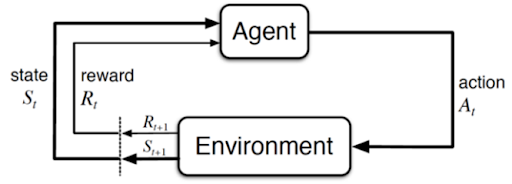
\includegraphics[width=.5\textwidth]{resources/img/markov_decision_process.png}
	\caption{Markov decision process: an iterative process in which an agent interacts with an environment (represented by its state at iteration $t$ $S_t$). The environment provides the agent with a set of possible actions $\{A_t^1, ..., A_t^{\alpha}\}$, the agent selects an action $A_t$, is rewarded with $R_t$ and the environment state is updated. The agents objective is to maximize its total reward $\sum_t R_t$.}
	\label{fig:mdp}
\end{figure}

In a Q-learning setting the target of the model is to predict the discounted reward obtained at the end of an "episode" if action $a_t$ is taken at iteration $t$. The objective we are trying to minimize is the difference between the predicted discounted reward $\gamma_{\theta}(a_t | P_t)$ and the incured reward plus the best discounted predicted reward in state $t+1$: $r_{a_t} + \lambda \max_{a\in A_{t+1}} \gamma_{\theta}(a | P_{t+1})$ .

In the MIS setting we can define:
\begin{itemize}
	\item State $S_t$: bipartite/factor-graph representation of the problem at current iteration (restriction to graph induced by remaining candidate vertices $W_t$)
	\item Actions are $W_t$
	\item All actions result is a reward $R_t = 1$
	\item Current implementations of our Nair+MRF models use the Sum-Product algorithm for producing estimated marginals $\mu_F(x_F)$. Replacing the Sum-Product by Max-Sum the estimations become max-pseudo-marginals $\Phi_F(x_F) = \max_{x': x'=x_F} E(x)$. We have shown that their exists an sequence of MRFs converging to with $E(x) \propto c(x)$ for $x\in\mathcal{F}$ and $E(x) = 0$ for $x\notin \mathcal{F}$. 
\end{itemize}


\section{Wasserstein distance unsupervised} Reinforcement learning can suffer from unstable learning, especially with sparse rewards. Although the MIS problem seems particularly well suited for this framework it might not be the case for other problems. In this section we present an outline of an unsupervised training method based on ranking and using the Wasserstein distance. Given a CO problem $P$ with cost function $c(x)$ with finite value on the feasible set $\mathcal{F}$ and $c(x)=\infty$ if $x\notin \mathcal{F}$ and a set of solutions $\{ x_i \}_{i\in\mathbb{N}}$, the idea is to train a MRF based model to imitate the ordering defined by $c(x)$. 

Assume that the target distribution is $p^*(x) \propto \exp c(x)$ and the model we want to fit is $p_{\theta}(x) \propto \exp \langle \theta , \phi(x) \rangle$. 


\newpage
\pagecolor{Wheat1}
\chapter{Appendix B}
\label{appendix_b}

\section{Clique cover construction.}  
Finding all maximal cliques is itself hard, but approximate coverings can be obtained efficiently. Algorithm~\ref{alg:clique_cover} sketches a simple constructive procedure for generating a clique cover.

\begin{algorithm}[H]
\caption{Covering a graph with maximal cliques}\label{alg:clique_cover}
\KwData{$G = (V,E)$}
\KwResult{Set of cliques $\mathcal{C} = \{ c : c\subseteq V \}$}
$\mathcal{C} = \emptyset$\;
$m(u,v) = 0 \quad \forall (u,v) \in E$\;
\While{$E \neq \emptyset$}{
  $c \gets$ select edge $(u,v)$ with $m(u,v)=0$\;
  $W = N(u) \cap N(v)$\;
  \While{$ W \neq \emptyset$}{
      $w \gets$ select in $W$\;
      $C \gets C \cup \{ w \}$\;
      $W = W \cap N(w)$\;
      $m(w,u) = 1 \quad \forall u \in C$\;
  }
  $\mathcal{C} \gets \mathcal{C} \cup \{ C \}$\;
}
\end{algorithm}


\end{appendices}

\newpage
\pagecolor{lightmauve}
\chapter{Appendix C}
\label{appendix_c}

\section{Inferring MIS solutions without training, alternate sampling methods and results}

This appendix complements the main results by examining two ablation variants in which we \emph{do not train} the MRF parameters. Instead, factor potentials are set deterministically from feasibility information and then used with fixed-iteration message passing to produce beliefs, which are decoded either greedily or via importance sampling (IS). These experiments isolate the value of learned potentials by asking: how far can one go with handcrafted feasibility-driven potentials on loopy factor graphs?

\paragraph{Common setting.}
We use the same MIS instance families and graph encodings as in the main text. For each partial assignment (during decoding), we update potentials according to the rules described below and then run sum–product (SP) or max–sum (MS) belief propagation for a fixed number of iterations with light damping; on loopy graphs, convergence is \emph{not} guaranteed and we report the last iterate. Decoding uses either a greedy policy guided by unary beliefs or IS with the beliefs serving as proposal/weights, consistent with the main experimental protocol.

\subsection{Variant A: Soft Feasibility Penalty (Nonzero Potentials)}
\label{app:soft_penalty}
\textbf{Definition.}
Let $x_\alpha$ be a local assignment for factor $\alpha$ (e.g., a clique or constraint scope). Define a simple violation indicator $v_\alpha(x_\alpha)\in\{0,1\}$ that is $1$ if $x_\alpha$ conflicts with the current partial solution or violates the local combinatorial constraint, and $0$ otherwise. We assign
\[
\psi_\alpha(x_\alpha) \;=\; 
\begin{cases}
\eta_{\text{feas}} & \text{if } v_\alpha(x_\alpha)=0,\\[2pt]
\eta_{\text{inf}}  & \text{if } v_\alpha(x_\alpha)=1,
\end{cases}
\qquad \text{with } \; 0<\eta_{\text{inf}}<\eta_{\text{feas}}.
\]
All assignments remain \emph{strictly} positive, but infeasible ones are down-weighted. In practice we use a fixed ratio $\eta_{\text{feas}}/\eta_{\text{inf}}>1$ to maintain numerical stability while biasing beliefs toward feasibility.

\textbf{Rationale.}
This “soft mask’’ encourages feasibility without collapsing potentials to zero, which can stall message passing or create brittle dynamics when many factors simultaneously rule out large portions of the local state space.

\textbf{Results and interpretation.}
Table~\ref{tab:soft_penalty_results} (Appendix) reports gaps for SP/MS with greedy and IS decoders. Trends are consistent across formulations: SP+IS improves upon SP+greedy, but both remain \emph{substantially} worse than trained models; MS is generally less stable and inferior here. Overall, keeping all assignments marginally viable does not compensate for the lack of learned, instance-adapted potentials; feasibility structure alone is too weak to drive high-quality solutions on loopy graphs.

\subsection{Variant B: Unary-Only Updates (Higher-Order Potentials Frozen)}
\label{app:unary_only}
\textbf{Definition.}
When a partial assignment fixes a subset of variables, we only modify \emph{unary} factors to reflect those fixed values (and optionally light preferences for unfixed variables), while \emph{keeping all higher-order factors unchanged}. This preserves computational simplicity and avoids repeatedly reconfiguring large factor tables during decoding.

\textbf{Rationale.}
This variant tests whether inexpensive potential updates can suffice when the factor graph is complex. It is attractive computationally, but it abandons the opportunity to re-encode evolving feasibility at the constraint level.

\textbf{Results and interpretation.}
Table~\ref{tab:unary_only_results} (Appendix) summarizes performance by formulation category. Unary-only updates yield the lowest overhead but also the weakest guidance: gaps remain high for both SP and MS; SP+IS is consistently better than SP+greedy yet still far from trained MRFs. Freezing higher-order factors deprives inference of the very constraint coupling it needs to steer decoding away from combinatorial conflicts.

\subsection{Discussion and Takeaways}
Across both ablations, we observe:
\begin{itemize}
  \item \textbf{No convergence guarantees.} On the loopy factor graphs considered, SP/MS often fail to converge; using a fixed number of iterations with damping mitigates but does not eliminate poor fixed points.
  \item \textbf{IS helps but is not sufficient.} Importance sampling on top of these untrained beliefs reliably improves gaps over greedy, yet it cannot close the gap to the learned models.
  \item \textbf{Learned structure is key.} Handcrafted feasibility signals—whether softly penalized or restricted to unaries—do not substitute for learned potentials that encode instance-specific structure. This reinforces the central claim of the paper: \emph{amortized, differentiable inference over a GNN-parameterized MRF materially improves solution quality}.
\end{itemize}

For numerical details, see Table~\ref{tab:soft_penalty_results} (soft feasibility penalty) and Table~\ref{tab:unary_only_results} (unary-only updates). Together with the main text, these ablations clarify that feasibility-only heuristics produce fragile beliefs and inferior solutions, whereas learning the MRF parameters—and running even a modest number of BP iterations—substantially boosts performance.


\begin{table}[!ht]
    \centering
    \begin{tabular}{l|r|r|r|r}
    \hline
        \textbf{Formulation} & \textbf{SP+Greedy} & \textbf{SP+IS} & \textbf{MS+Greedy} & \textbf{MS+IS} \\ \hline
        MIS100\_EB & $13.737 (\pm 4.925)$ & $\mathbf{6.478 (\pm 4.321)}$ & $37.001 (\pm 6.369)$ & $30.769 (\pm 6.411)$ \\
        MIS100\_CC & $14.186 (\pm 5.255)$ & $\mathbf{9.947 (\pm 4.827)}$ & $33.050 (\pm 7.347)$ & $28.603 (\pm 6.688)$ \\
        MIS100\_CF & $13.737 (\pm 4.925)$ & $\mathbf{6.478 (\pm 4.321)}$ & $37.001 (\pm 6.369)$ & $30.769 (\pm 6.411)$ \\
        MIS100\_EC & $13.971 (\pm 4.901)$ & $\mathbf{11.515 (\pm 4.679)}$ & $35.155 (\pm 6.708)$ & $30.112 (\pm 7.054)$ \\
        MIS100\_CP & $13.889 (\pm 5.456)$ & $\mathbf{9.872 (\pm 5.025)}$ & $33.454 (\pm 6.849)$ & $28.513 (\pm 6.556)$ \\ \hline
    \end{tabular}
    \caption{Optimality gap comparison for Sum-Product and Max-Sum belief propagation algorithm inference, with greedy and importance sampling (V2: only unary factor parameters are changed) solvers. The model is defined following the "idealized" models such as defined in \ref{equ:idealized_mrf} but parameters are set to values $\theta_{r:x_r}=1$ if $A_r^T x_r \leq b_r$ and $\theta_{r:x_r}=0$ otherwise.}
    \label{tab:soft_penalty_results}
\end{table}

\begin{table}[!ht]
    \centering
    \begin{tabular}{l||r|r|r|r}
    \hline
        \textbf{Cat} & \textbf{SP+Greedy} & \textbf{SP+IS} & \textbf{MS+Greedy} & \textbf{MS+IS} \\ \hline
        EB & $14.072 (\pm 4.576)$ & $\mathbf{4.500 (\pm 3.800)}$ & $13.220 (\pm 3.590)$ & $23.142 (\pm 7.354)$ \\
        CC & $11.518 (\pm 4.752)$ & $\mathbf{4.917 (\pm 4.761)}$ & $14.472 (\pm 3.856)$ & $25.174 (\pm 8.768)$ \\
        CF & $14.072 (\pm 4.576)$ & $\mathbf{4.500 (\pm 3.800)}$  & $13.220 (\pm 3.590)$ & $23.142 (\pm 7.354)$ \\
        EC & $21.056 (\pm 4.846)$ & $\mathbf{11.535 (\pm 4.726)}$ & $12.370 (\pm 4.449)$ & $25.991 (\pm 8.489)$ \\
        CP & $13.656 (\pm 4.238)$ & $\mathbf{5.351 (\pm 4.483)}$ & $13.222 (\pm 4.842)$ & $24.391 (\pm 9.750)$ \\ \hline
    \end{tabular}
    \caption{Optimality gap comparison for Sum-Product and Max-Sum belief propagation algorithm inference, with greedy and importance sampling (V2: only unary factor parameters are changed) solvers. The model is defined following the "idealized" models such as defined in \ref{equ:idealized_mrf}}
    \label{tab:unary_only_results}
\end{table}

\newpage
\pagecolor{lightmauve}
\chapter{Appendix D}
\label{appendix_d}

% equations before the algorithm
\begin{align}
r_{F \to Y_i}(y_i) &= \log \sum_{\substack{y'_F \in Y_F \\ y'_i = y_i}}
   \exp\!\left(-E_F(y'_F) + \sum_{j \in N(F)\setminus\{i\}} q_{Y_j \to F}(y'_j)\right), \label{eq:lbf_fac2var}\\
\bar q_{Y_i \to F}(y_i) &= \sum_{F' \in M(i)\setminus\{F\}} r_{F' \to Y_i}(y_i), \label{eq:lbf_var2fac_raw}\\
q_{Y_i \to F}(y_i) &= \bar q_{Y_i \to F}(y_i) -
   \log \sum_{y_i \in Y_i}\exp\!\big(\bar q_{Y_i \to F}(y_i)\big). \label{eq:lbf_var2fac}
\end{align}

% algorithm
\begin{algorithm}[H]
\caption{Loopy Belief Propagation (Sum–Product)}
\KwIn{$(V,F,E)$, energies $E_F$, tolerance $\varepsilon$, max iters $T$}
\KwOut{Beliefs $\mu_i$, $\mu_F$, approx.\ $\log Z$}
\BlankLine
Initialize $q_{Y_i\to F}(y_i)\gets 0$ for all edges and states\;
\For{$t=1$ \KwTo $T$}{
  Update all $r_{F \to Y_i}$ using \eqref{eq:lbf_fac2var}\;
  Update all $q_{Y_i \to F}$ using \eqref{eq:lbf_var2fac_raw}–\eqref{eq:lbf_var2fac}\;
  Update beliefs $\mu_F,\mu_i$ (see text)\;
  \If{beliefs change $<\varepsilon$}{break}
}
Compute $\log Z$ via Bethe free energy (Eq.~\eqref{eq:bethe})\;
\end{algorithm}



\cleardoublepage
\addcontentsline{toc}{chapter}{INDEX}
\pagecolor{white}
\printindex

\end{document}
